% =================================
\section{画面遷移図}
% =================================

\subsection{学習者画面}

学習者用画面の画面遷移図を以下の図\ref{fig:lerner}に示す。

\begin{figure}[H]
  \centering
  \includegraphics[width=\linewidth]{chapters/images/UI_Screen/lerner/lerner.png}
  \caption{学習者画面遷移図}
  \label{fig:lerner}
\end{figure}

\subsection{投稿者画面}

投稿者画面の画面遷移図を以下の図\ref{fig:teacher}に示す。

\begin{figure}[H]
  \centering
  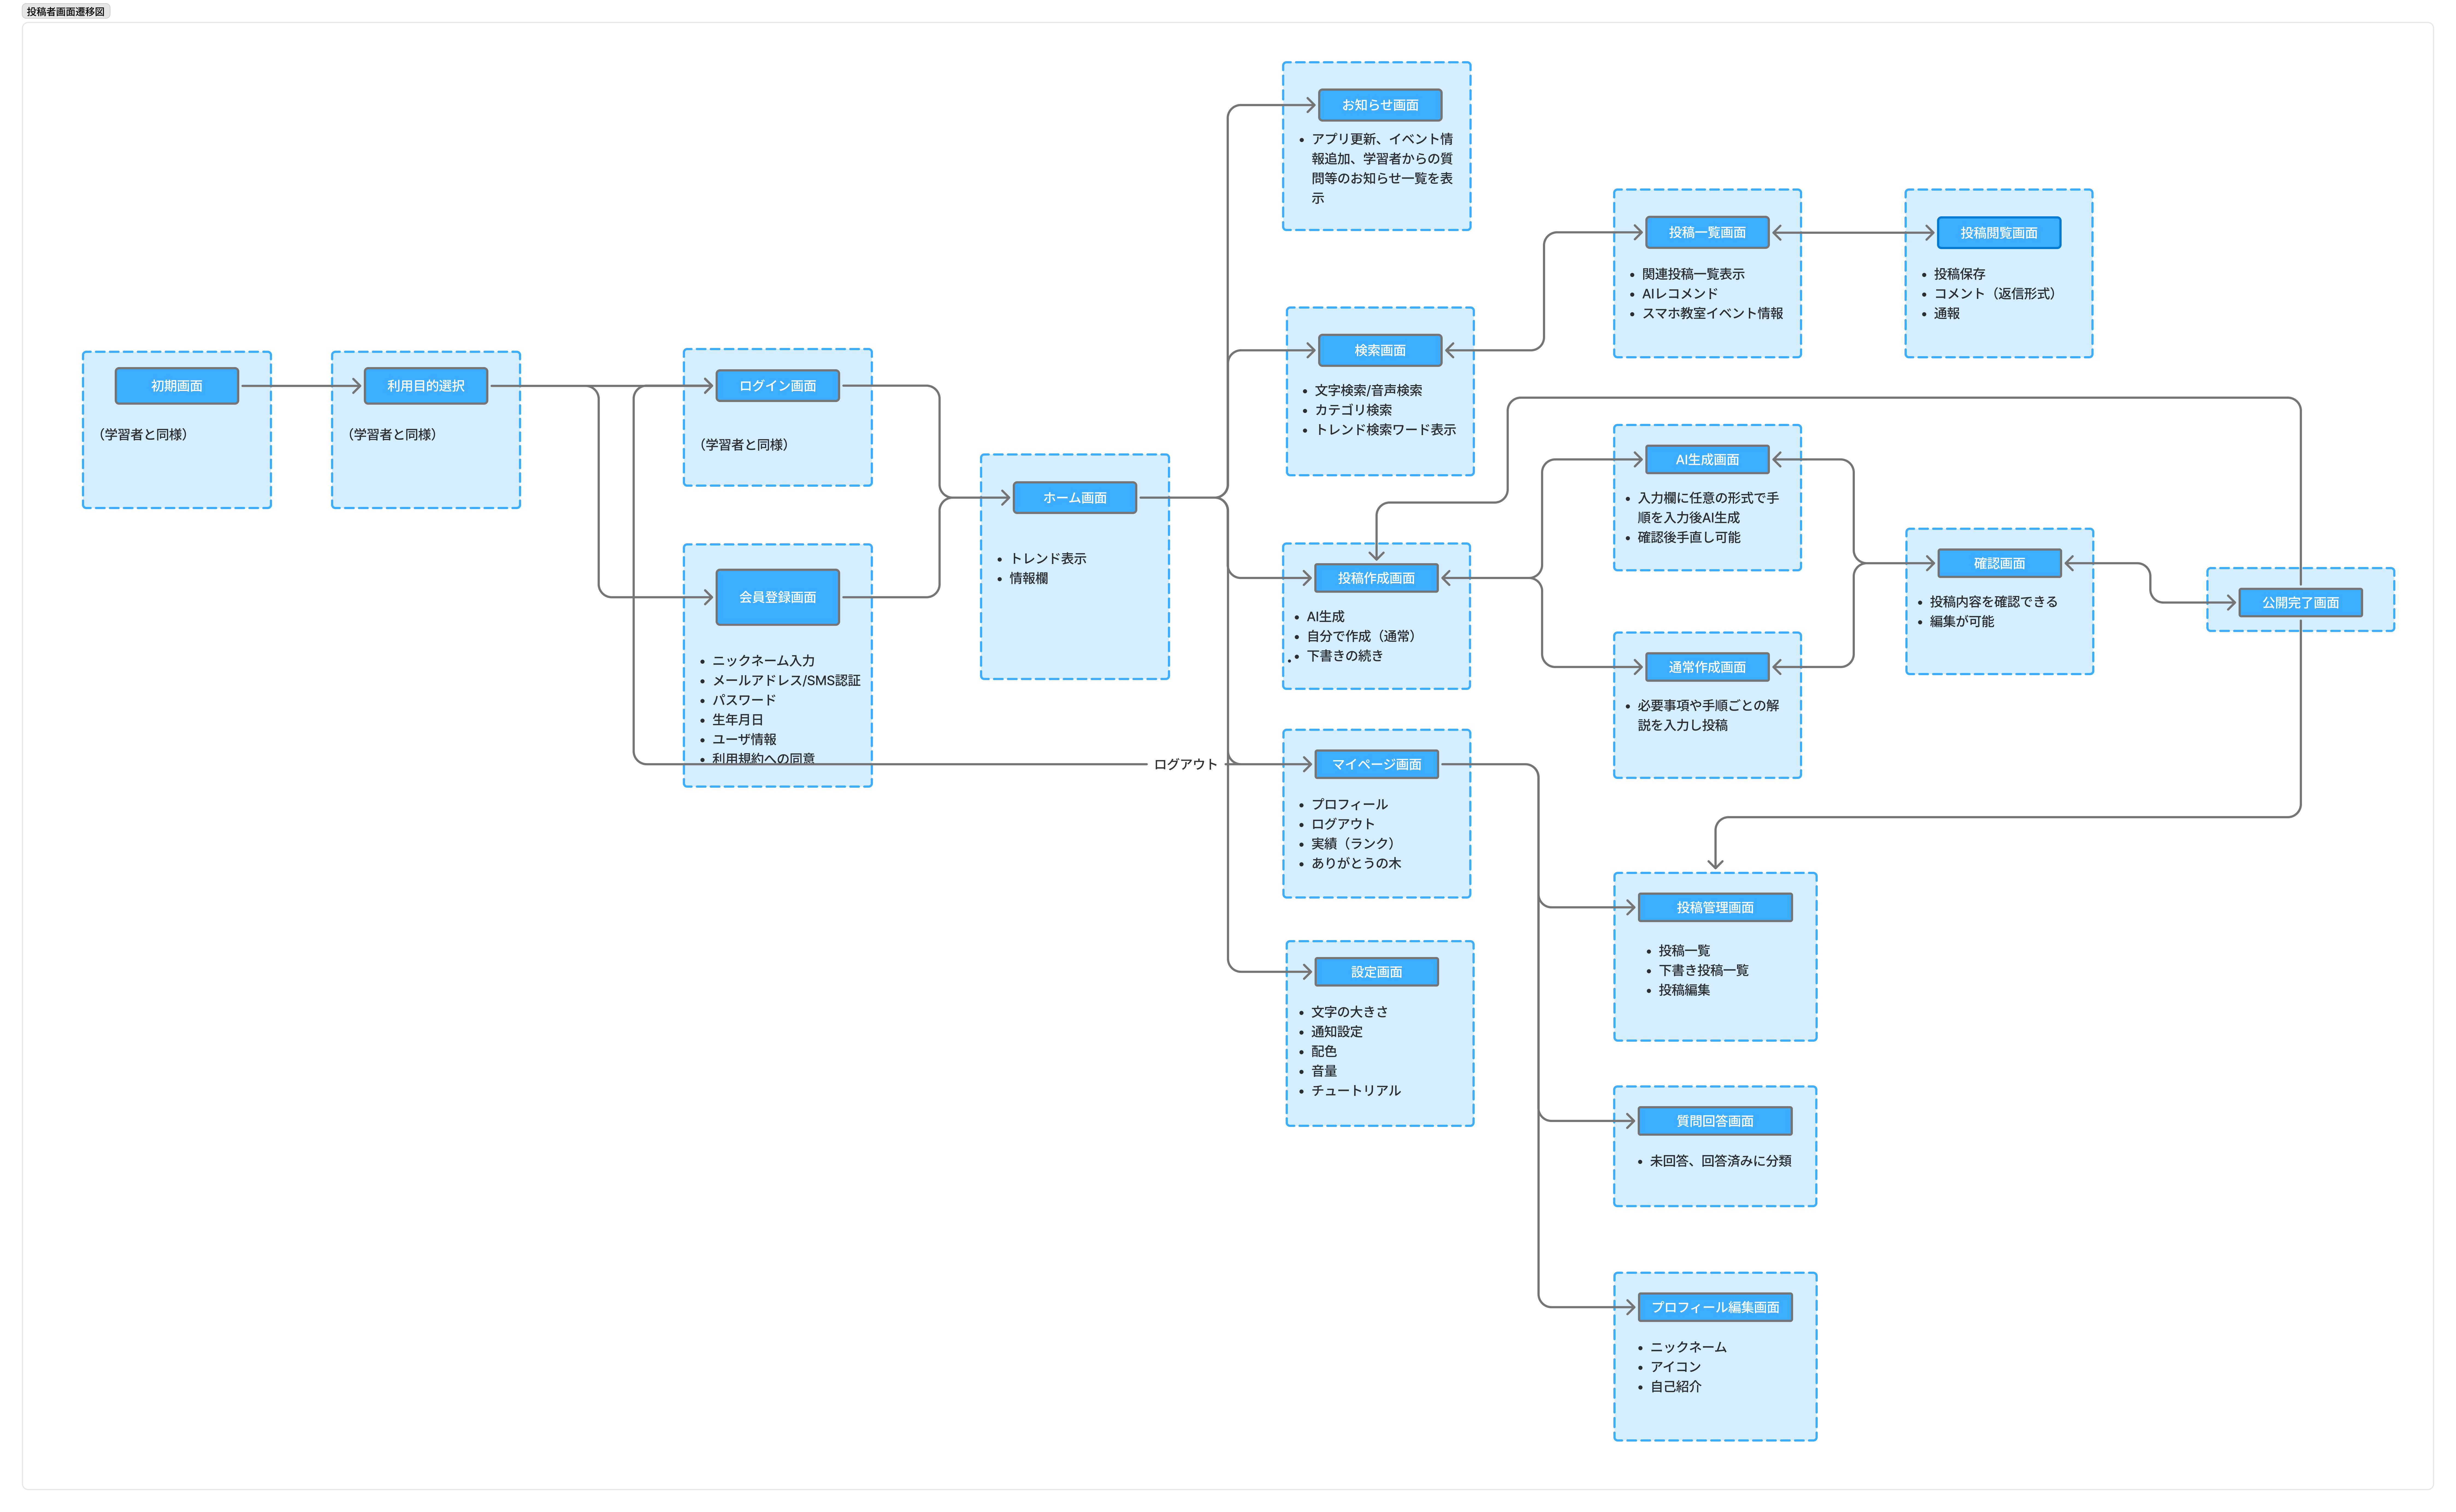
\includegraphics[width=\linewidth]{chapters/images/UI_Screen/teacher/teacher.png}
  \caption{投稿者画面遷移図}
  \label{fig:teacher}
\end{figure}

\subsection{管理者画面}
管理者画面の画面遷移図を以下の図\ref{fig:admin}に示す。

\begin{figure}[H]
  \centering
  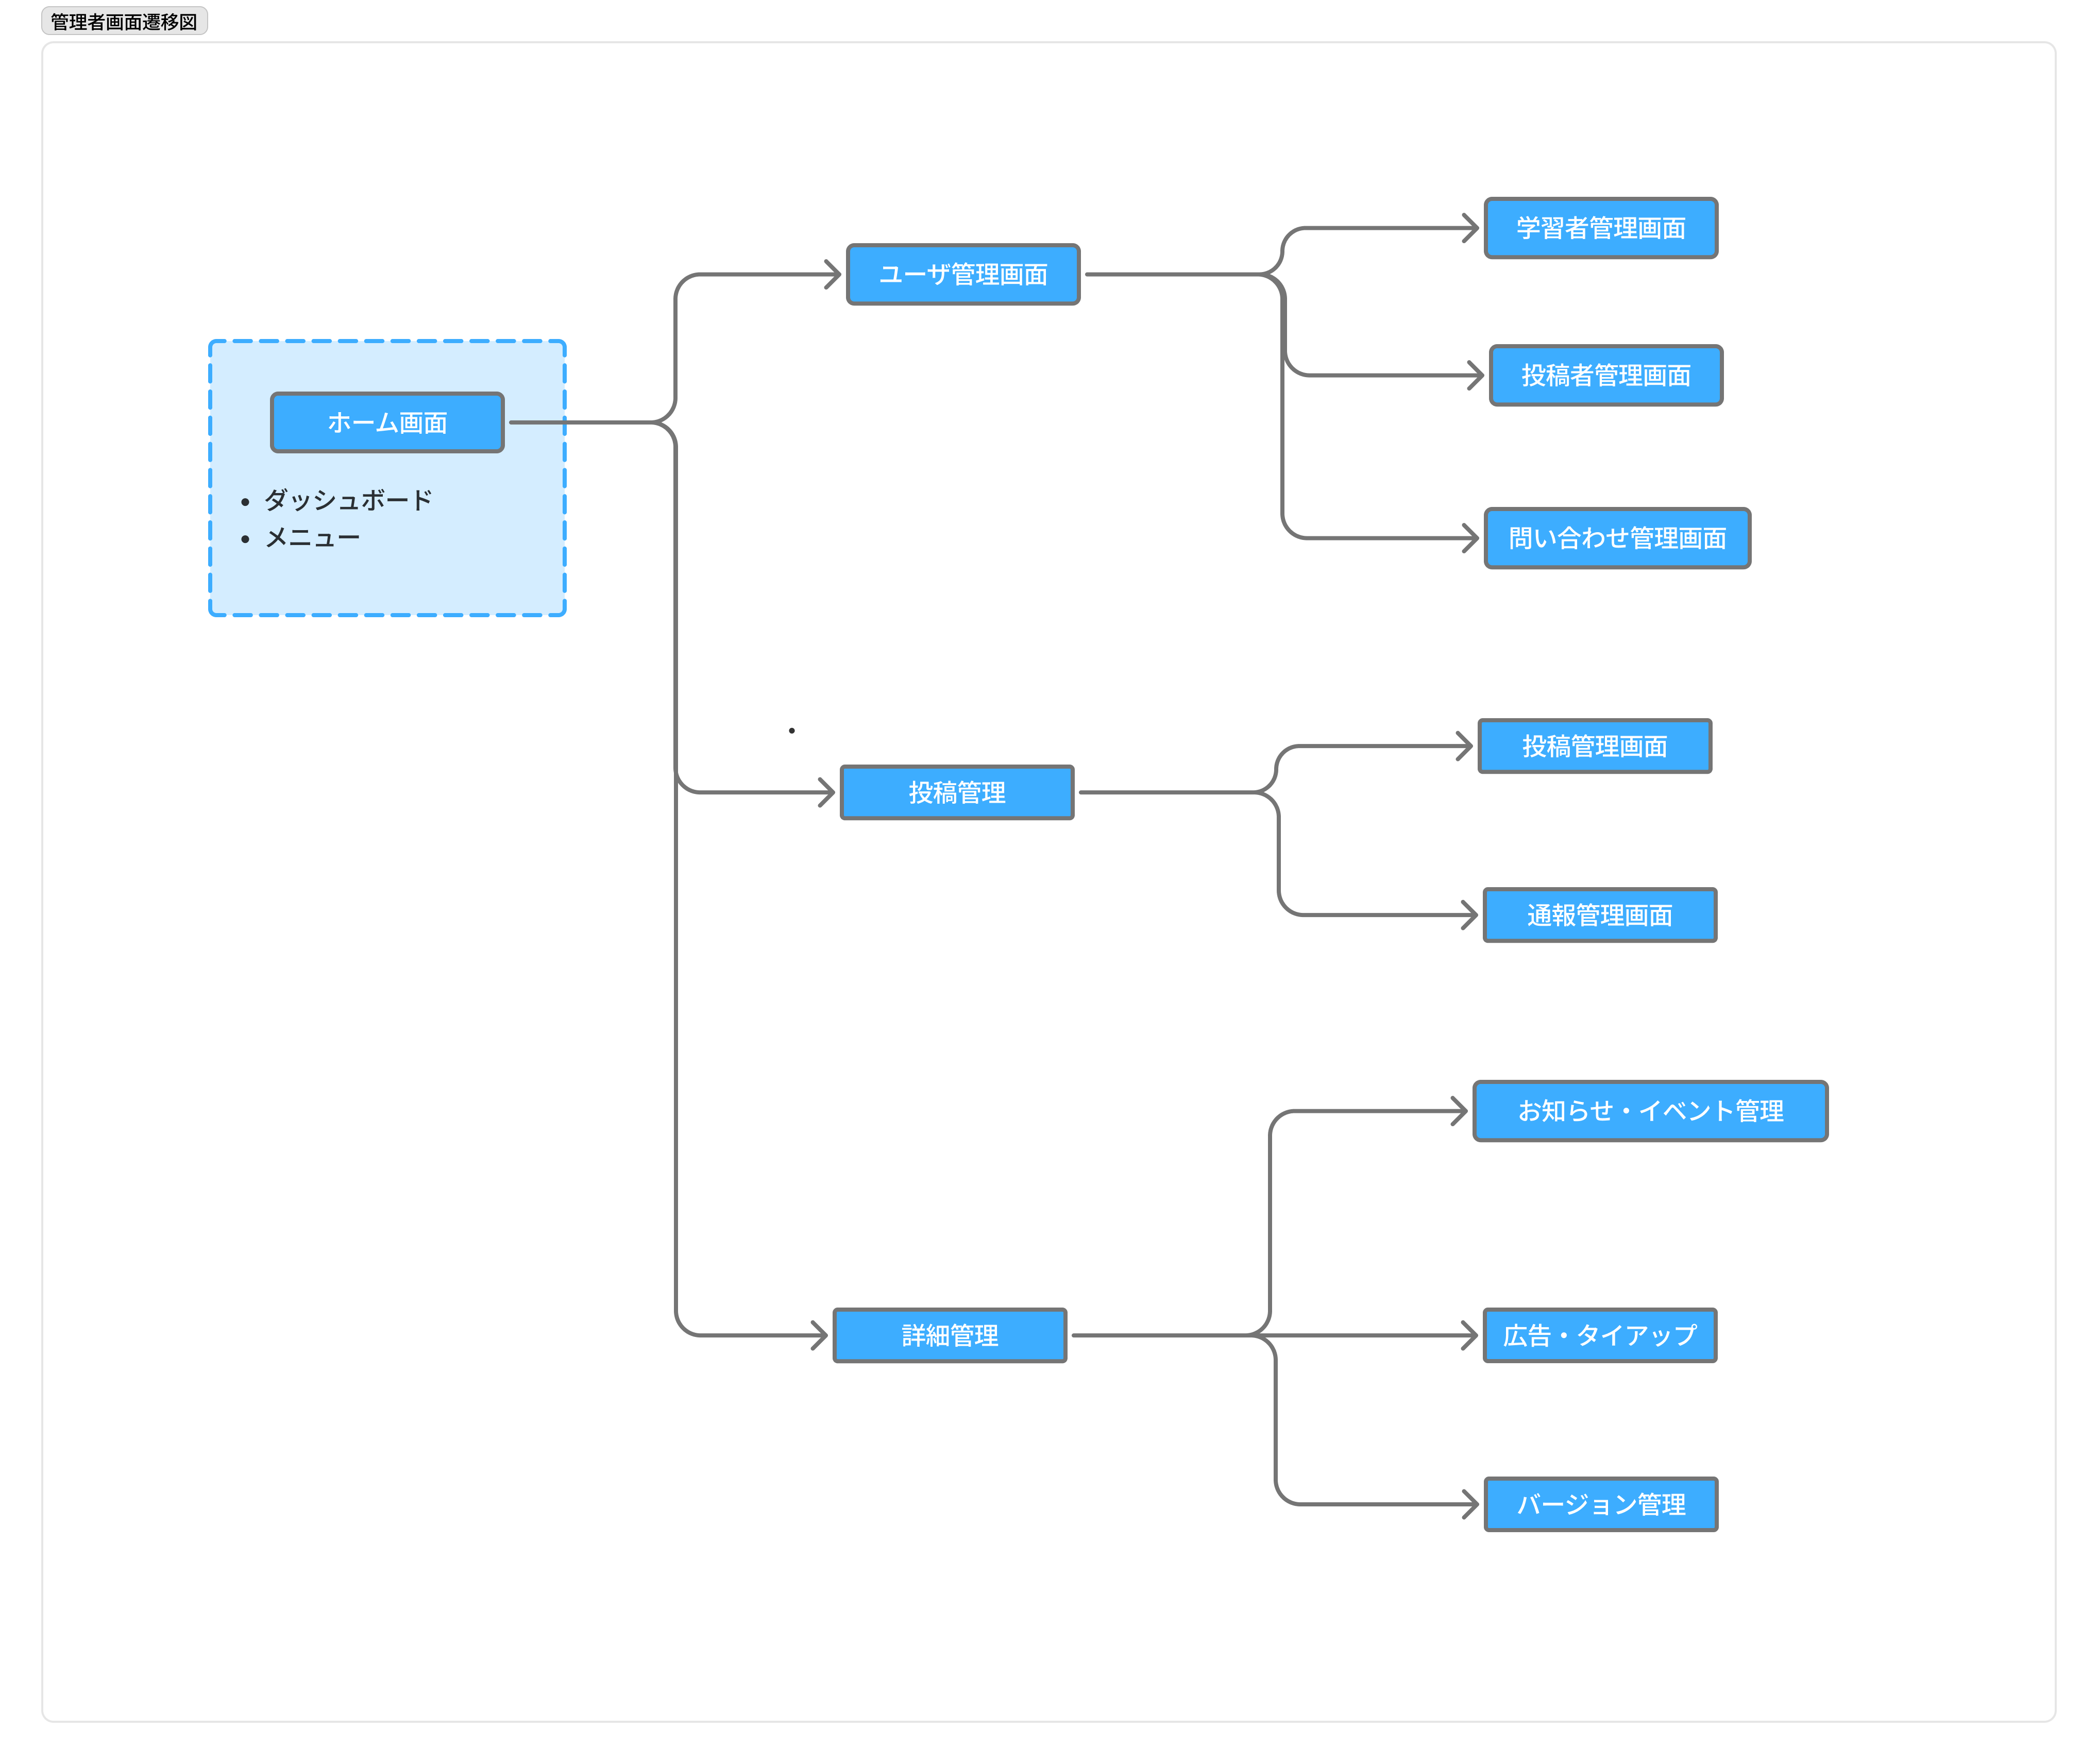
\includegraphics[width=\linewidth]{chapters/images/UI_Screen/admin/admin.png}
  \caption{管理者画面遷移図}
  \label{fig:admin}
\end{figure}

% =================================
\section{利用者向け画面}
% =================================

% =================================
\subsection{共通画面}
% =================================

\subsubsection{初期画面}

アプリの初期画面を図\ref{fig:start}に示す。

\begin{figure}[H]
  \centering

  \begin{subfigure}[t]{0.31\linewidth}
    \centering
    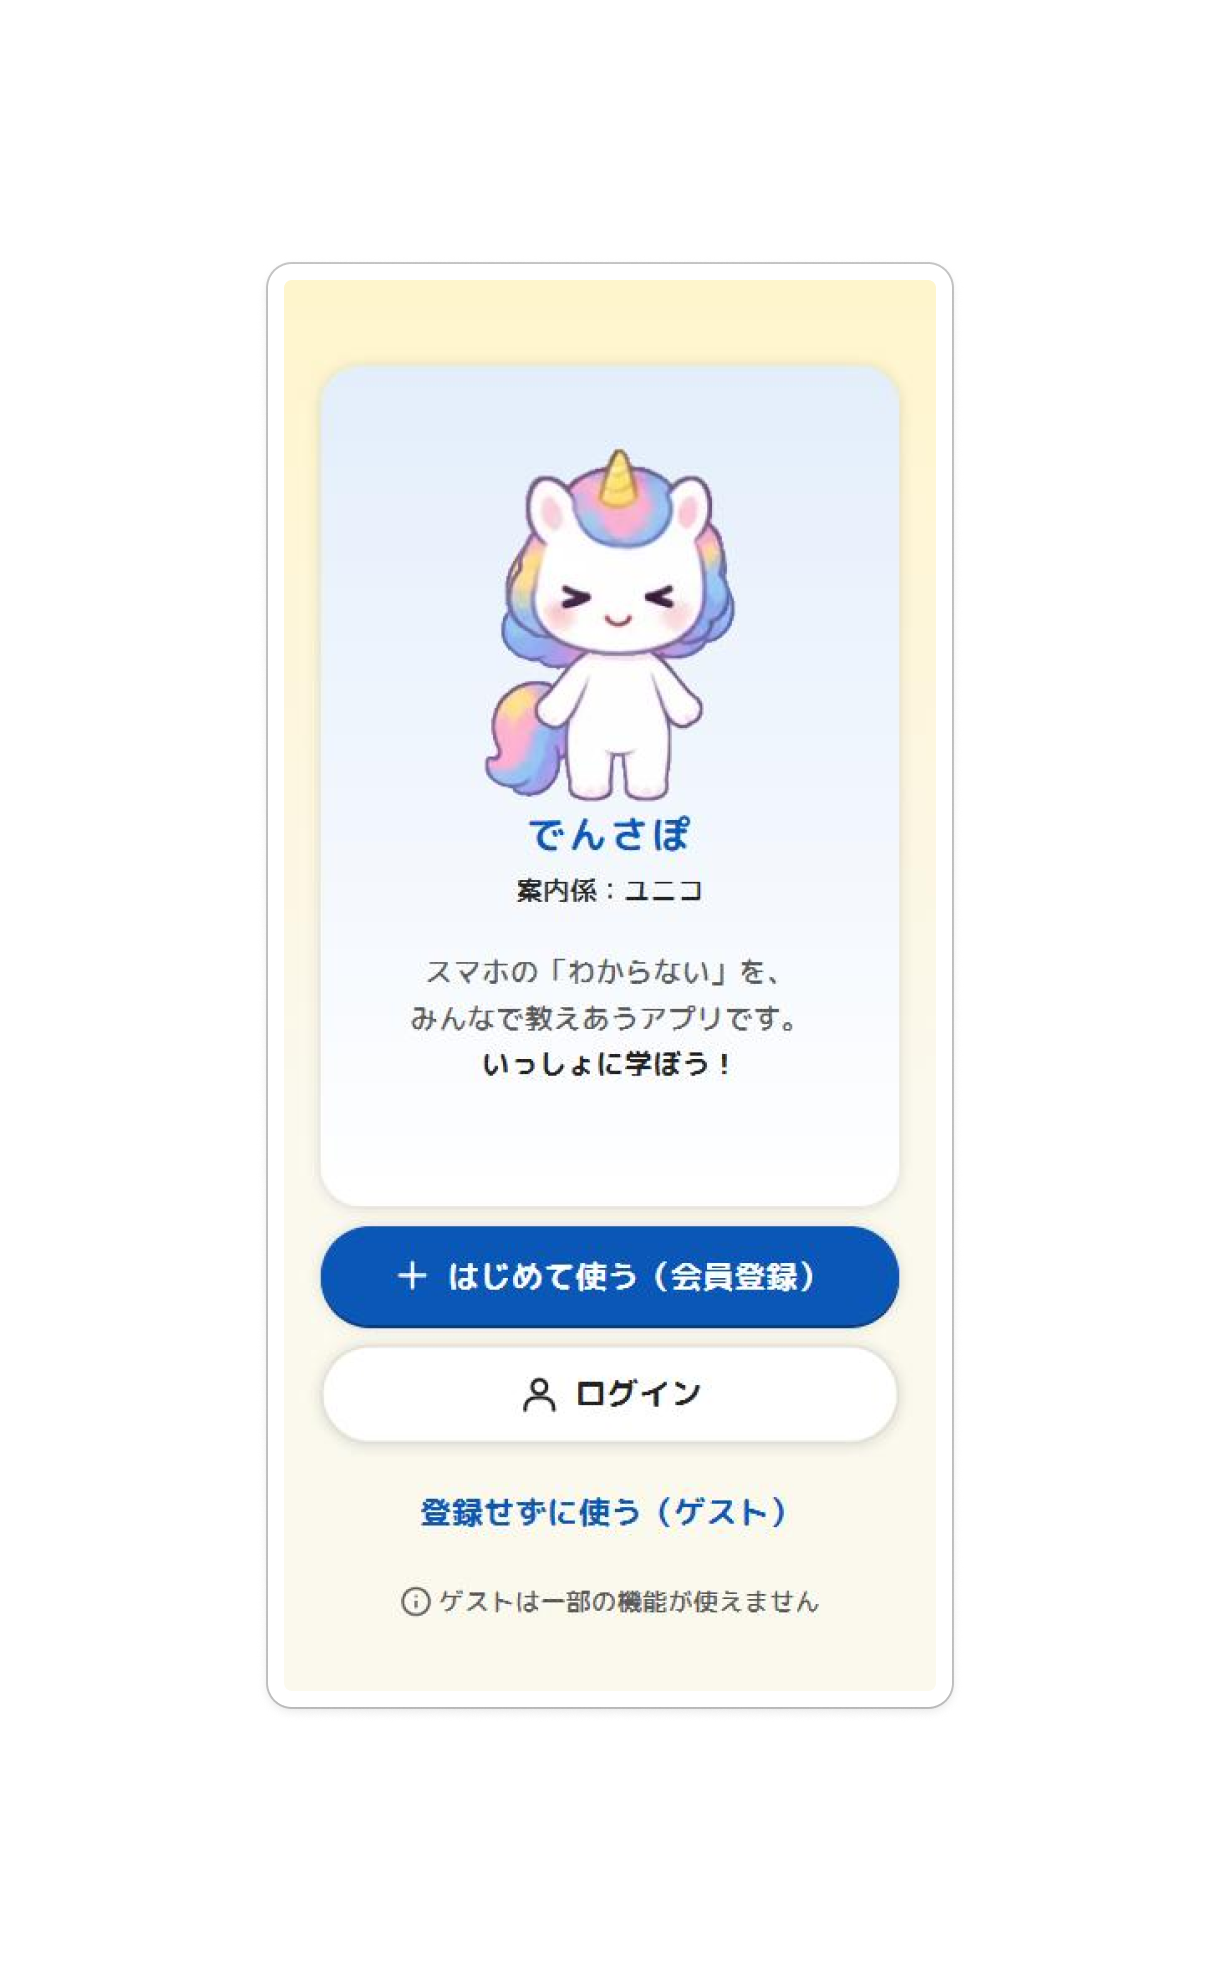
\includegraphics[width=\linewidth]{chapters/images/UI_Screen/start1.png}
    \caption{初期画面}
    \label{fig:start1}
  \end{subfigure}
  \hfill
  \begin{subfigure}[t]{0.31\linewidth}
    \centering
    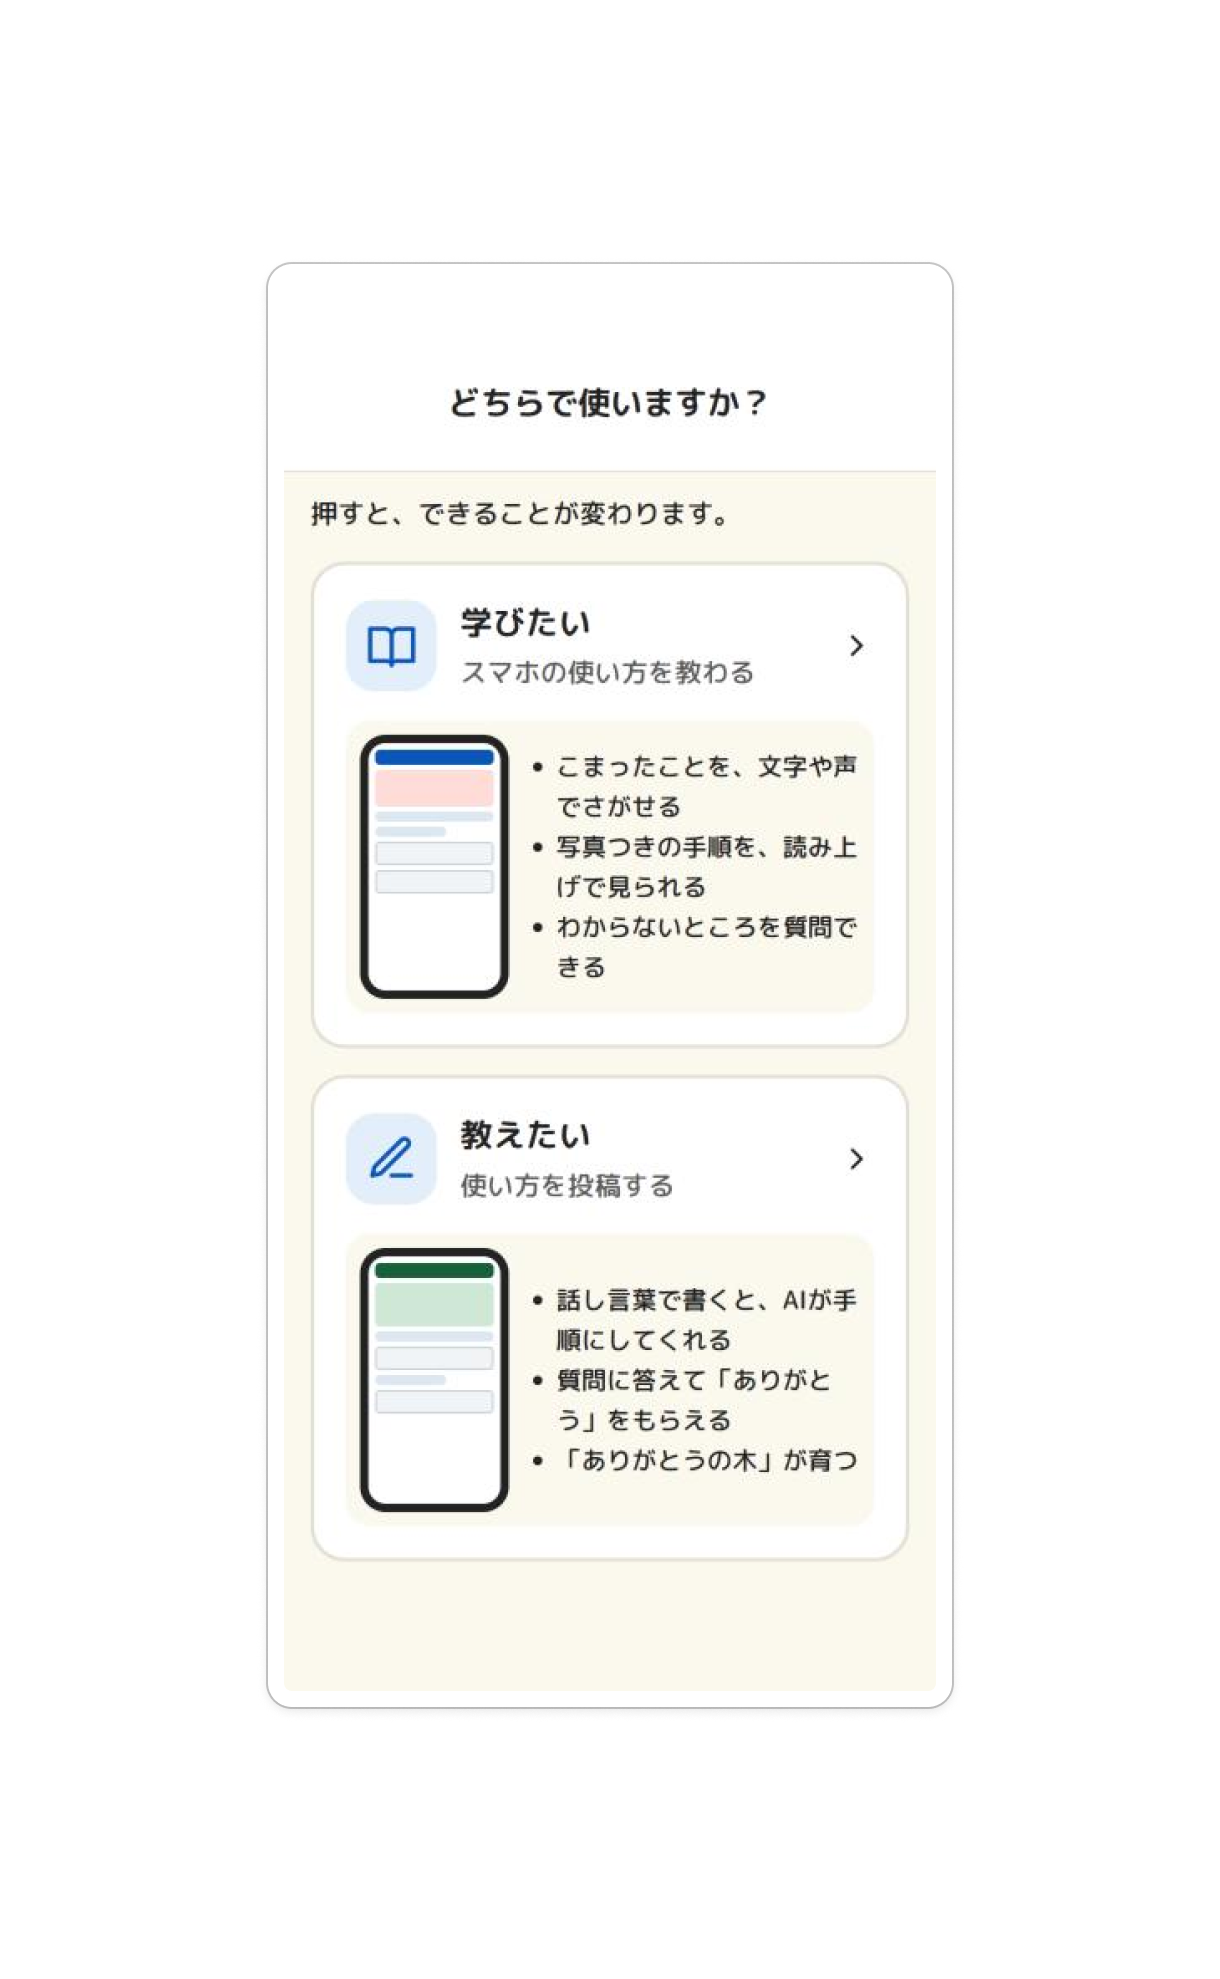
\includegraphics[width=\linewidth]{chapters/images/UI_Screen/start2.png}
    \caption{利用目的選択画面}
    \label{fig:start2}
  \end{subfigure}
  \hfill
  \begin{subfigure}[t]{0.31\linewidth}
    \centering
    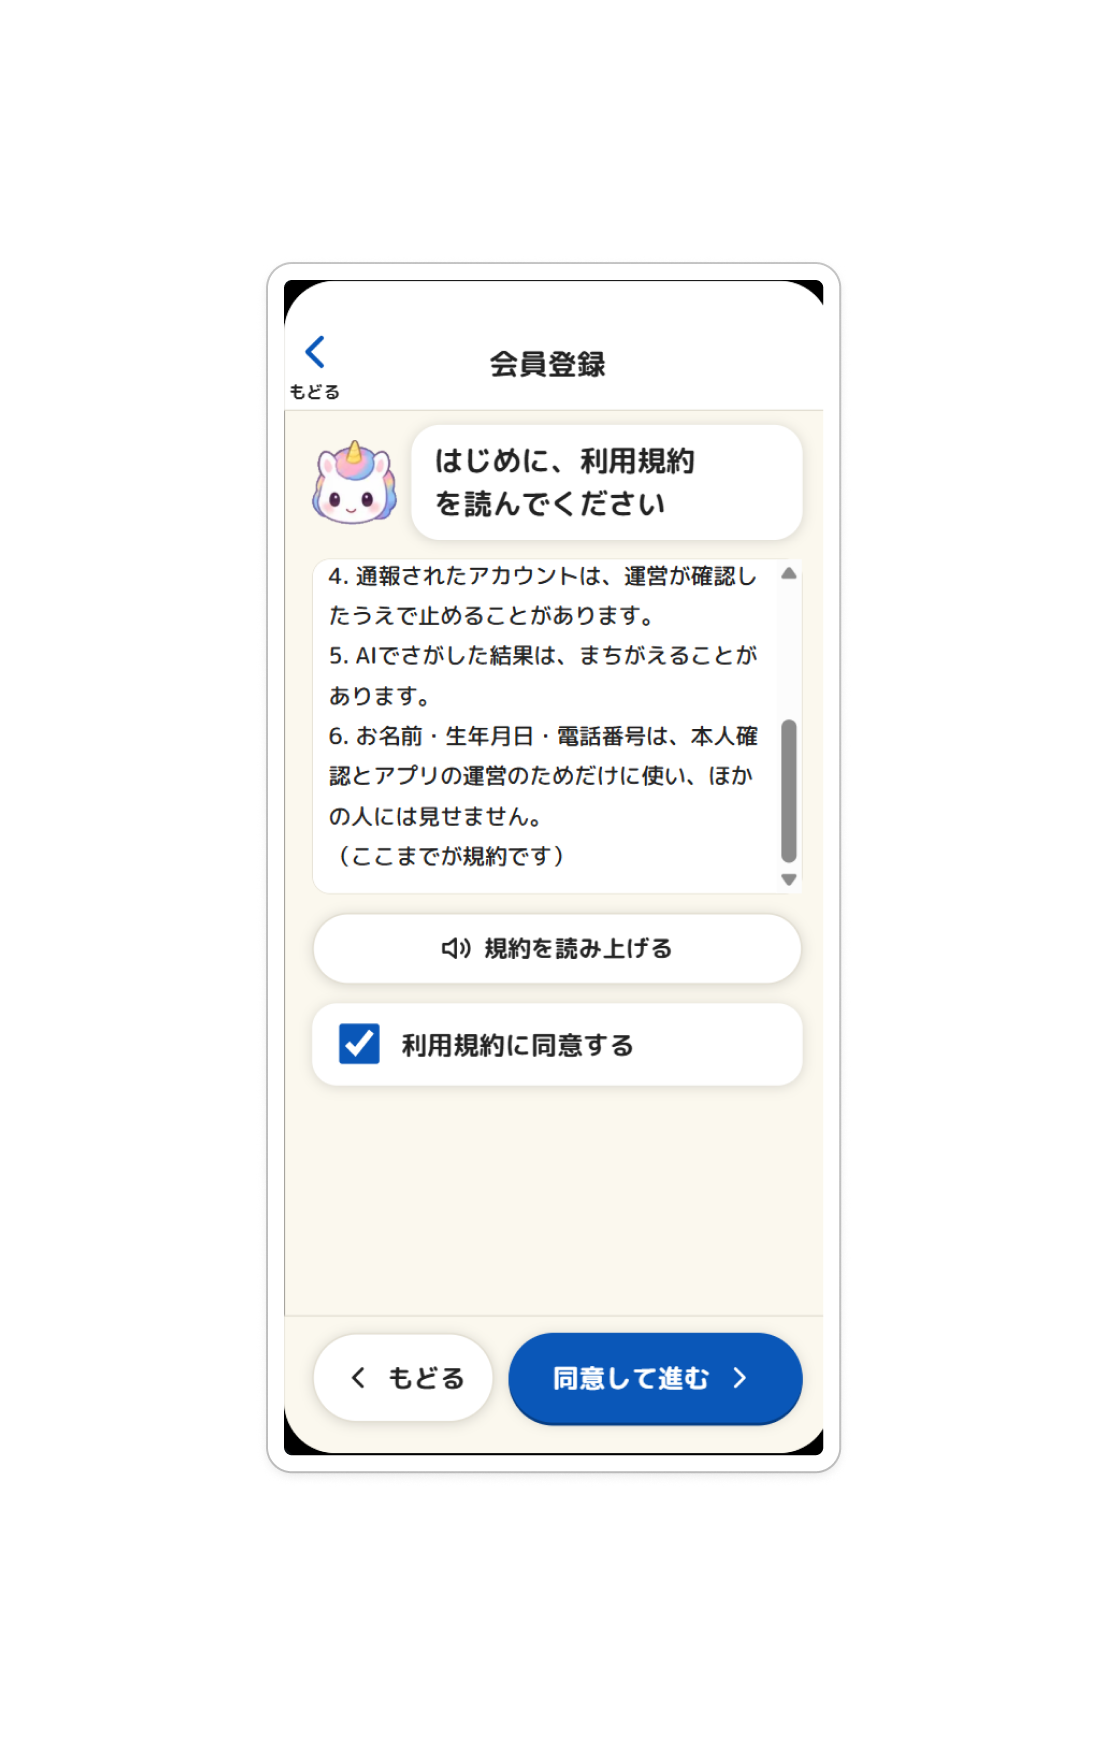
\includegraphics[width=\linewidth]{chapters/images/UI_Screen/start3.png}
    \caption{会員登録同意画面}
    \label{fig:start3}
  \end{subfigure}

  \caption{初期画面}
  \label{fig:start}
\end{figure}

図\ref{fig:start1}は、アプリを初めて開いたときに表示する初期画面である。「はじめて使う（会員登録）」または「ログイン」をタップすると、利用目的の選択画面へ進む。「登録せずに使う（ゲスト）」をタップすると、登録せずにゲスト用ホーム画面へ進む。

図\ref{fig:start2}は、アプリの利用目的を選択する画面である。「学びたい」をタップすると学習者として、「教えたい」をタップすると投稿者として、会員登録またはログインへ進む。

図\ref{fig:start3}は、会員登録に同意する画面である。最後までスクロール後、チェックボックスをタップすることで次の画面へ進む。


% =================================
\subsubsection{会員登録画面}
% =================================

会員登録画面は、各項目をステップごとに回答していく画面である。会員登録画面を図\ref{fig:reg}に示す。

\begin{figure}[H]
  \centering

  % 1～3
  \begin{subfigure}[t]{0.31\linewidth}
    \centering
    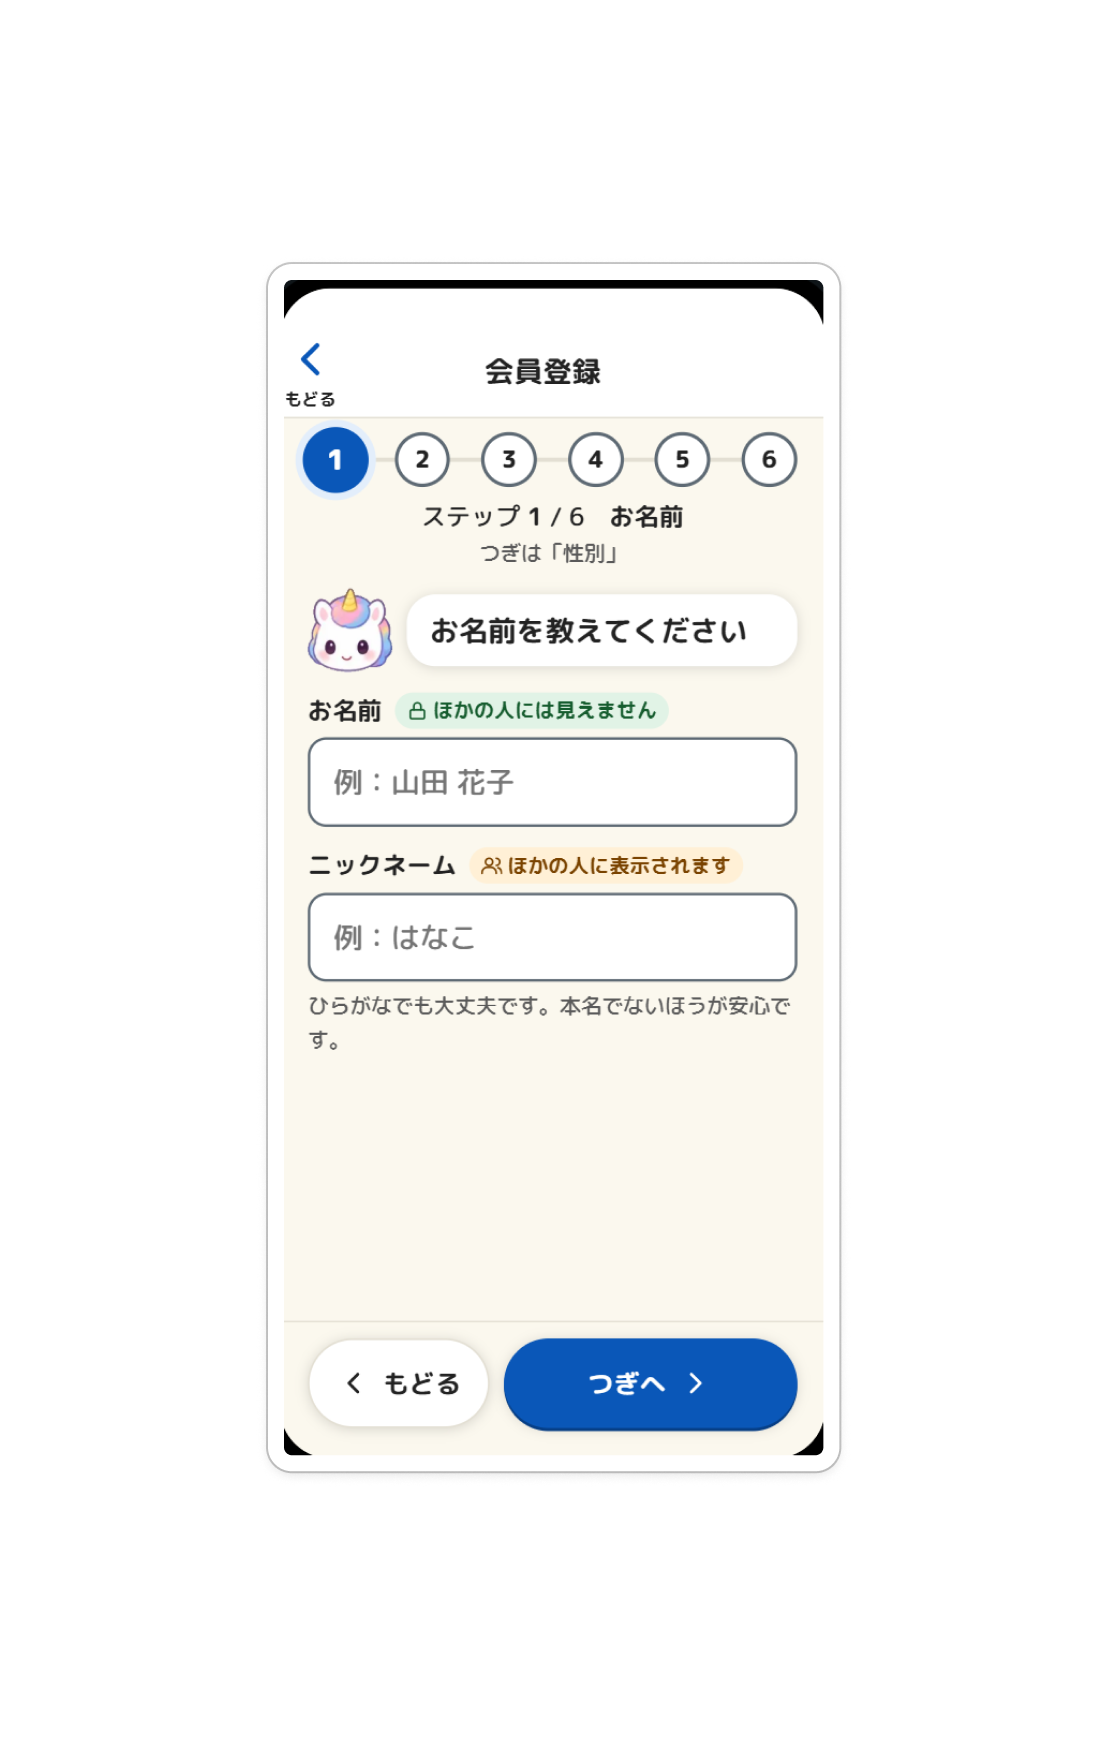
\includegraphics[width=\linewidth]{chapters/images/UI_Screen/reg1.png}
    \caption{名前入力画面}
    \label{fig:reg1}
  \end{subfigure}
  \hfill
  \begin{subfigure}[t]{0.31\linewidth}
    \centering
    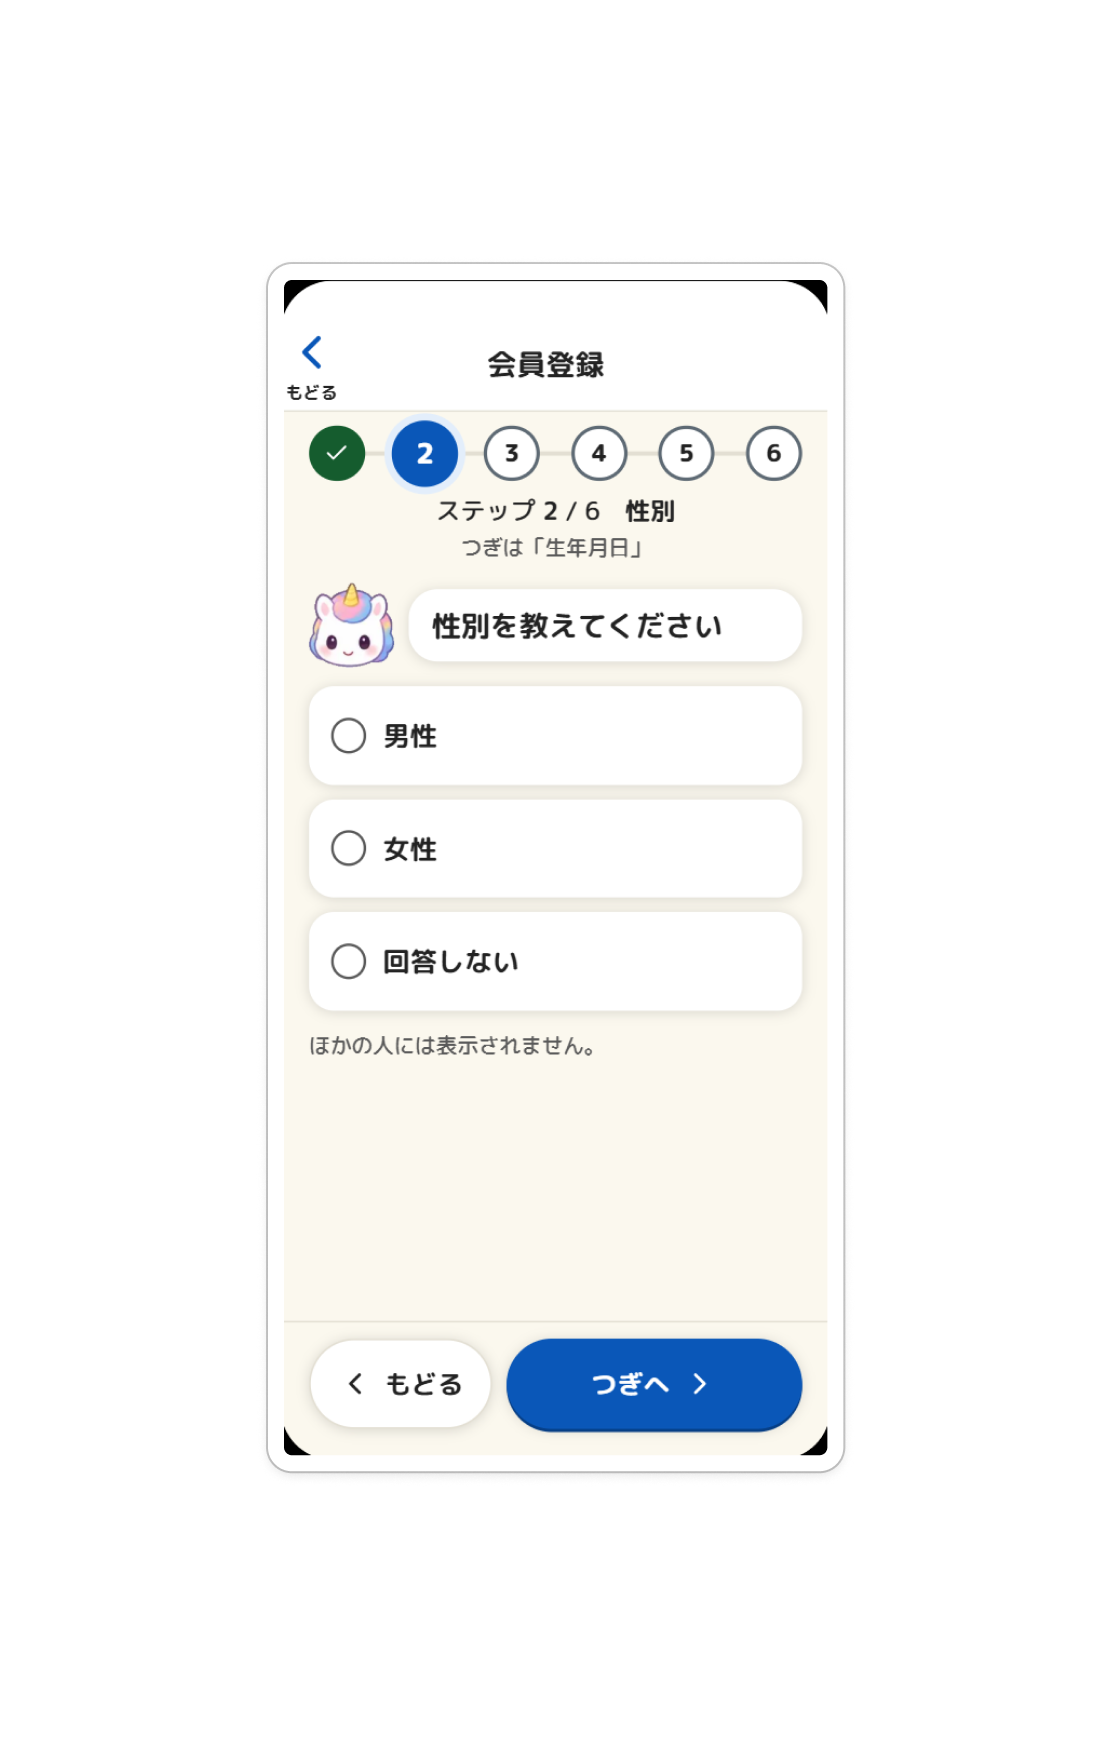
\includegraphics[width=\linewidth]{chapters/images/UI_Screen/reg2.png}
    \caption{性別入力画面}
    \label{fig:reg2}
  \end{subfigure}
  \hfill
  \begin{subfigure}[t]{0.31\linewidth}
    \centering
    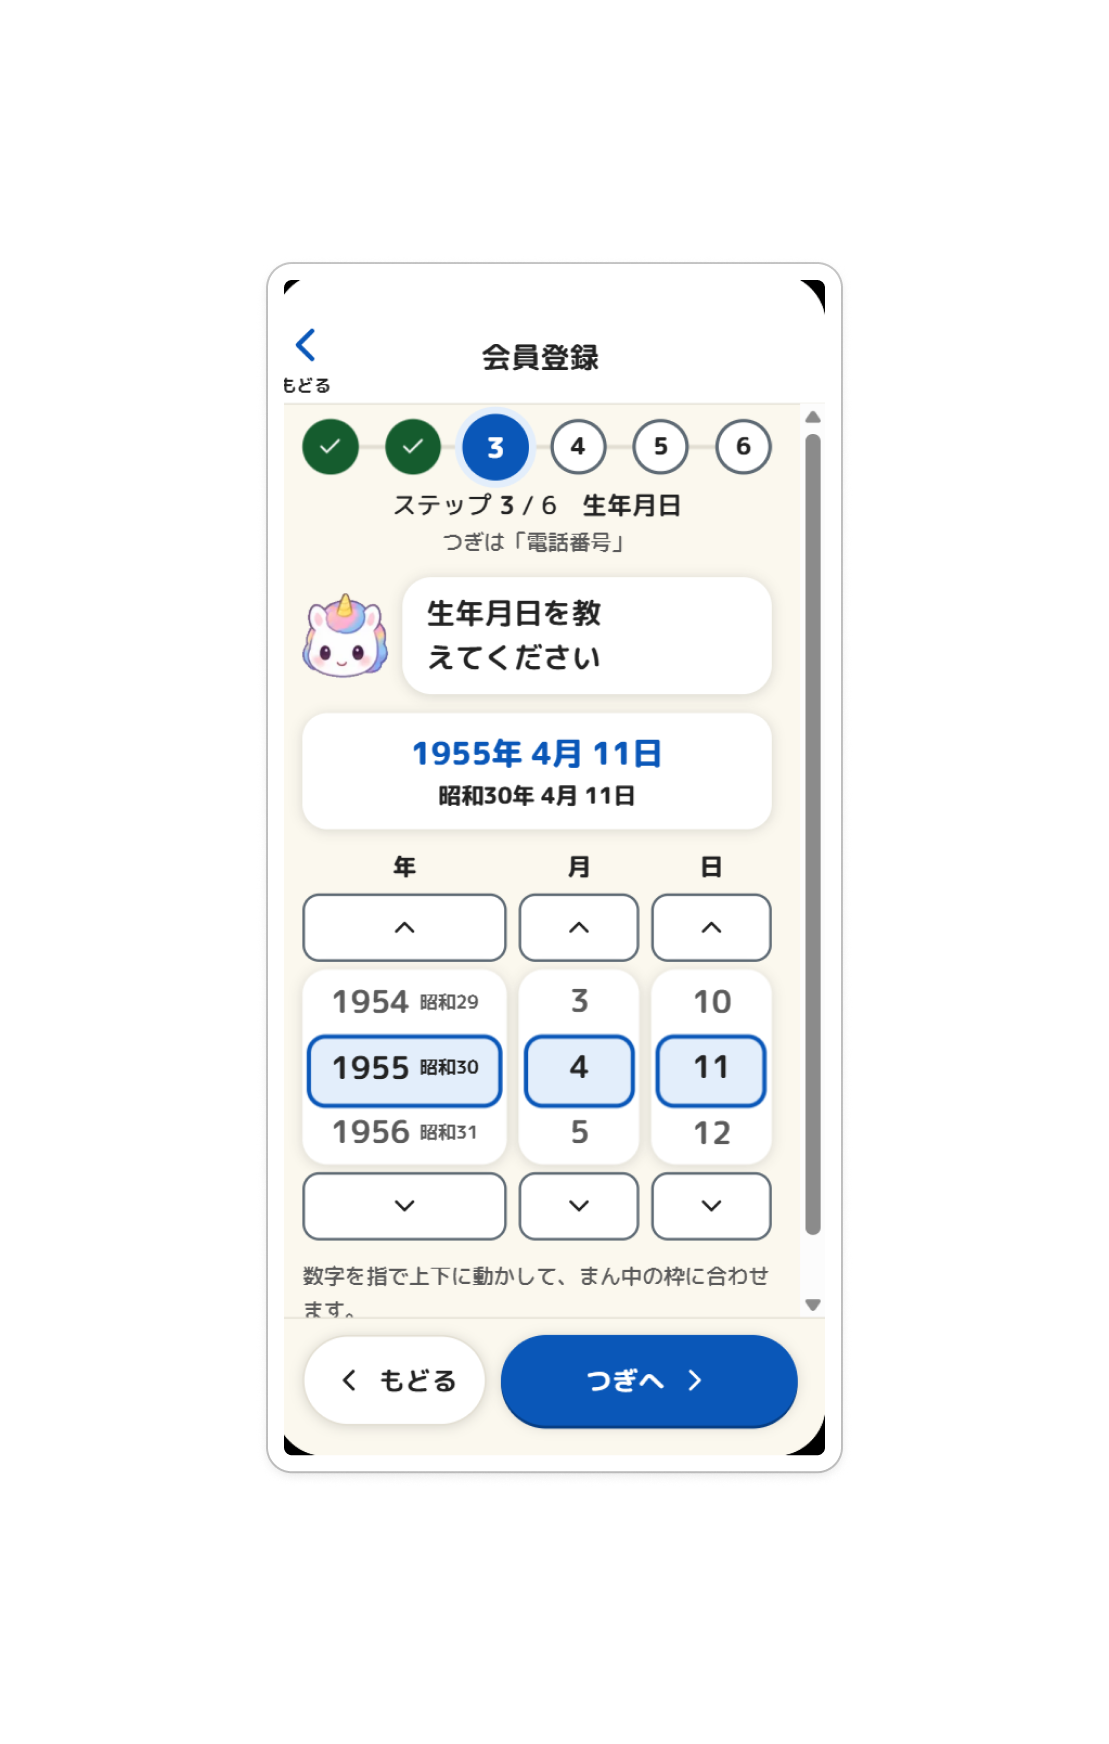
\includegraphics[width=\linewidth]{chapters/images/UI_Screen/reg3.png}
    \caption{生年月日入力画面}
    \label{fig:reg3}
  \end{subfigure}

  \vspace{5mm}

  % 4～7
  \begin{subfigure}[t]{0.23\linewidth}
    \centering
    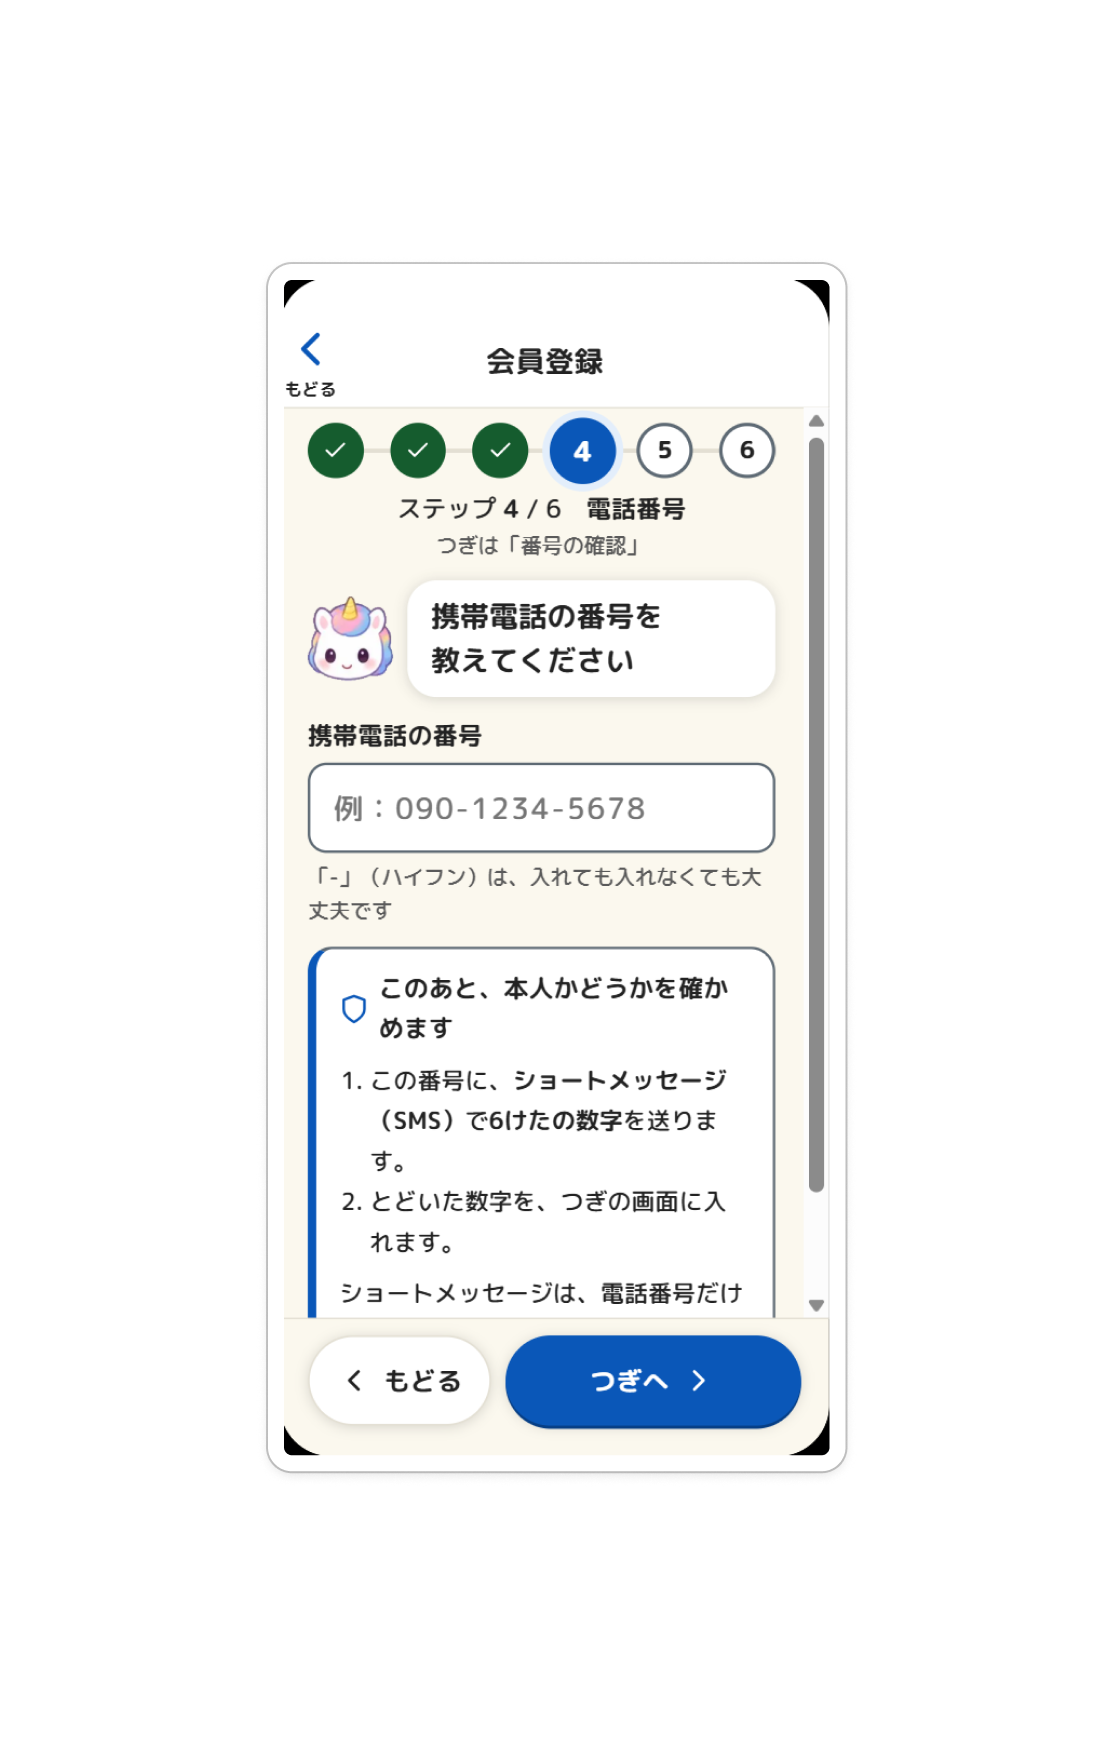
\includegraphics[width=\linewidth]{chapters/images/UI_Screen/reg4.png}
    \caption{電話番号入力画面}
    \label{fig:reg4}
  \end{subfigure}
  \hfill
  \begin{subfigure}[t]{0.23\linewidth}
    \centering
    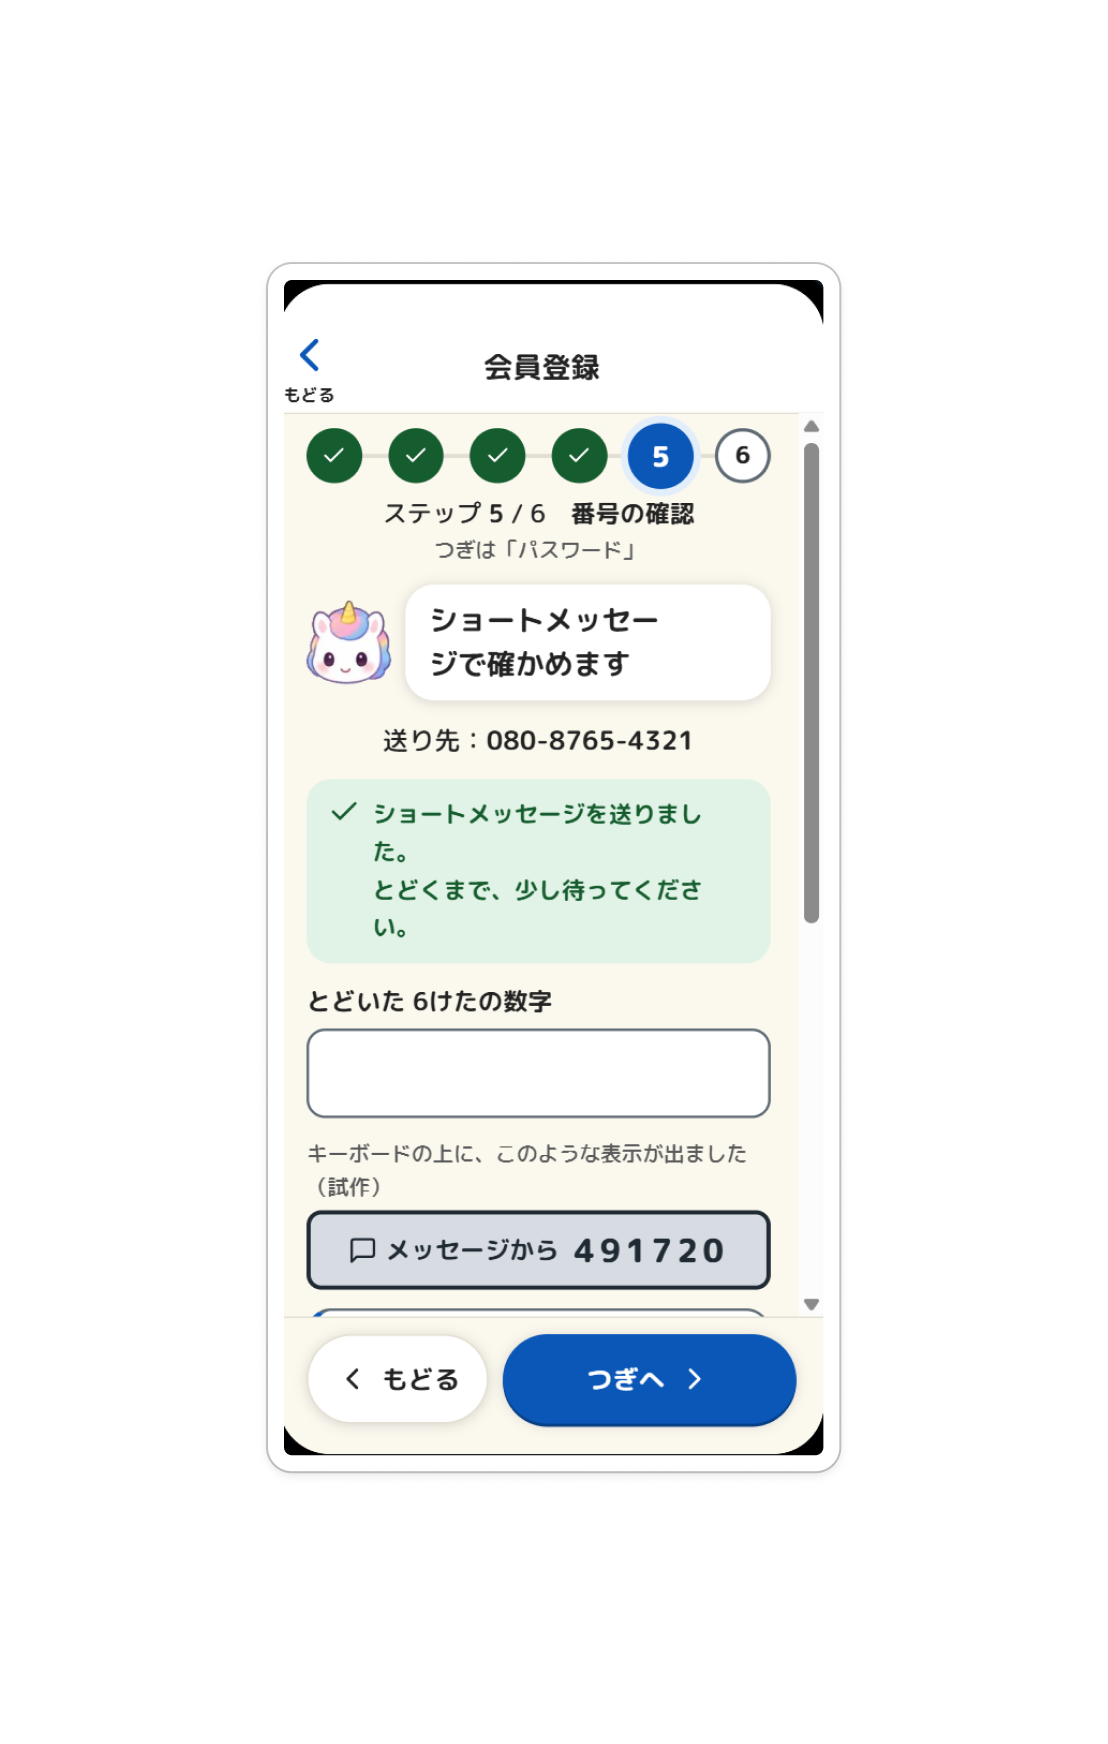
\includegraphics[width=\linewidth]{chapters/images/UI_Screen/reg5.png}
    \caption{SMS認証画面}
    \label{fig:reg5}
  \end{subfigure}
  \hfill
  \begin{subfigure}[t]{0.23\linewidth}
    \centering
    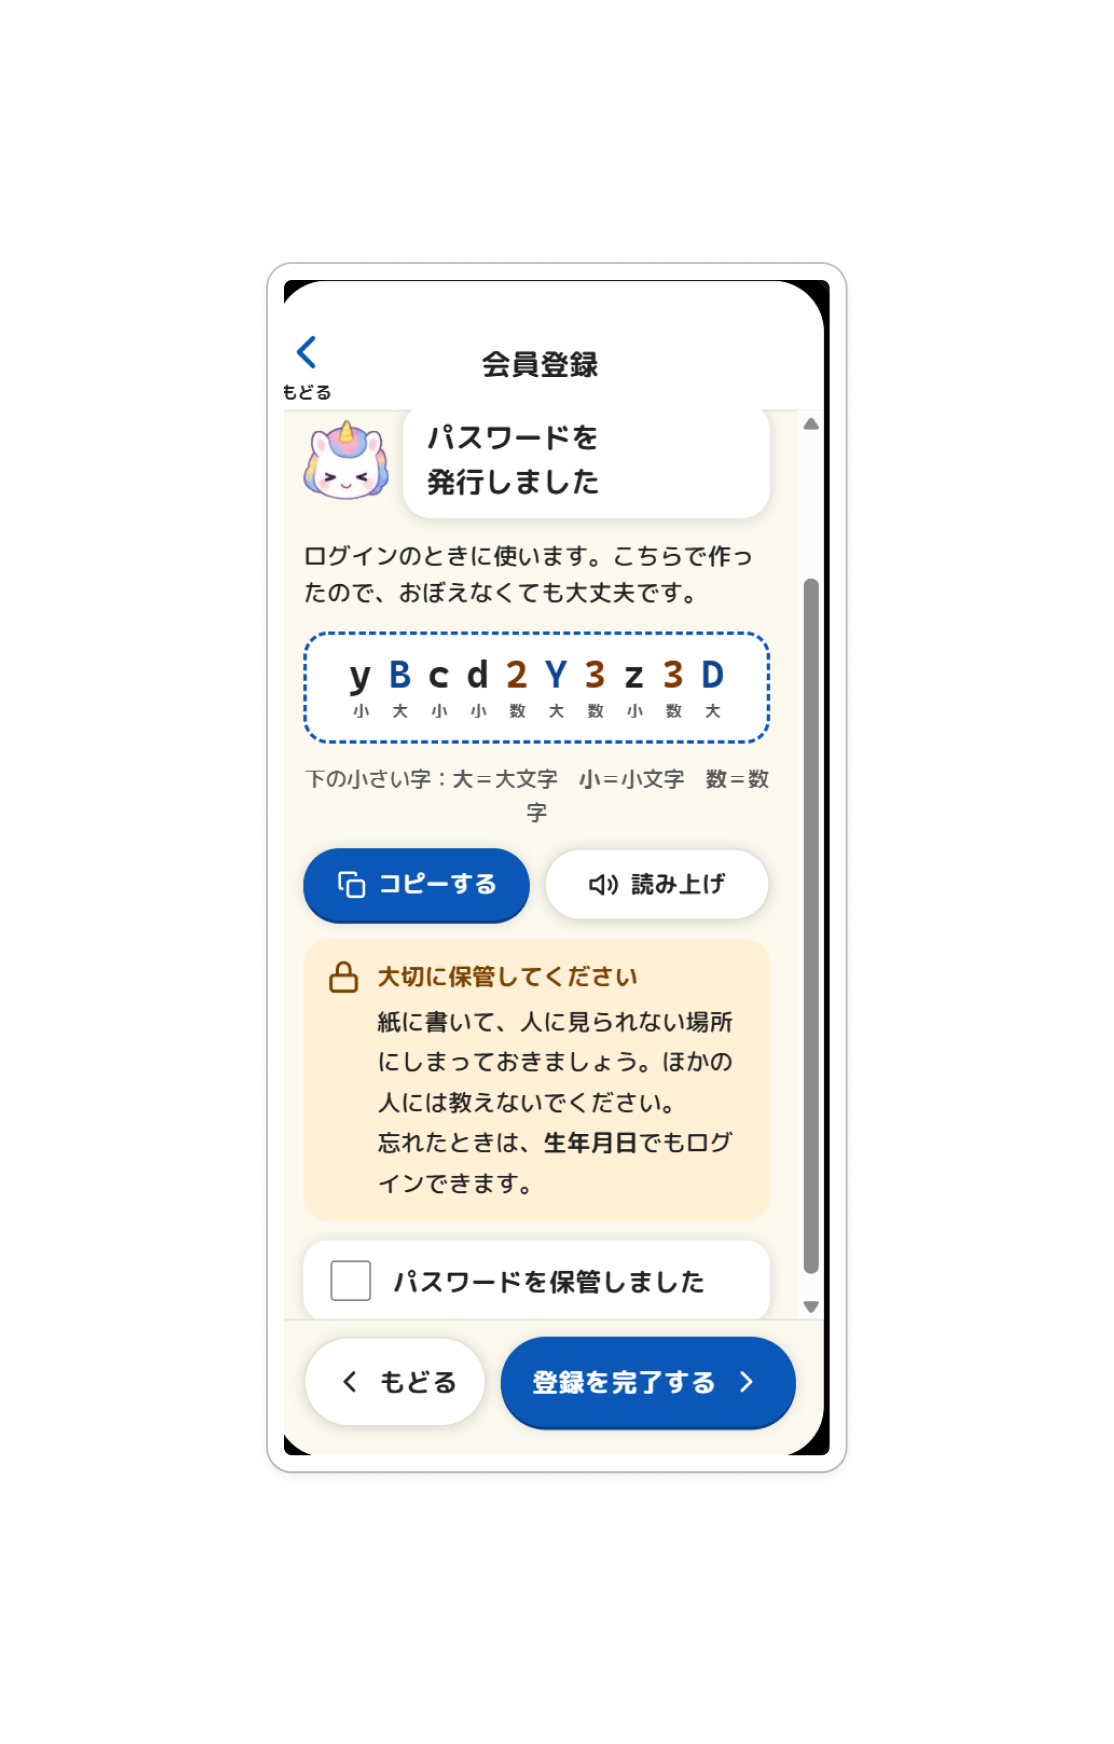
\includegraphics[width=\linewidth]{chapters/images/UI_Screen/reg6.png}
    \caption{パスワード発行画面}
    \label{fig:reg6}
  \end{subfigure}
  \hfill
  \begin{subfigure}[t]{0.23\linewidth}
    \centering
    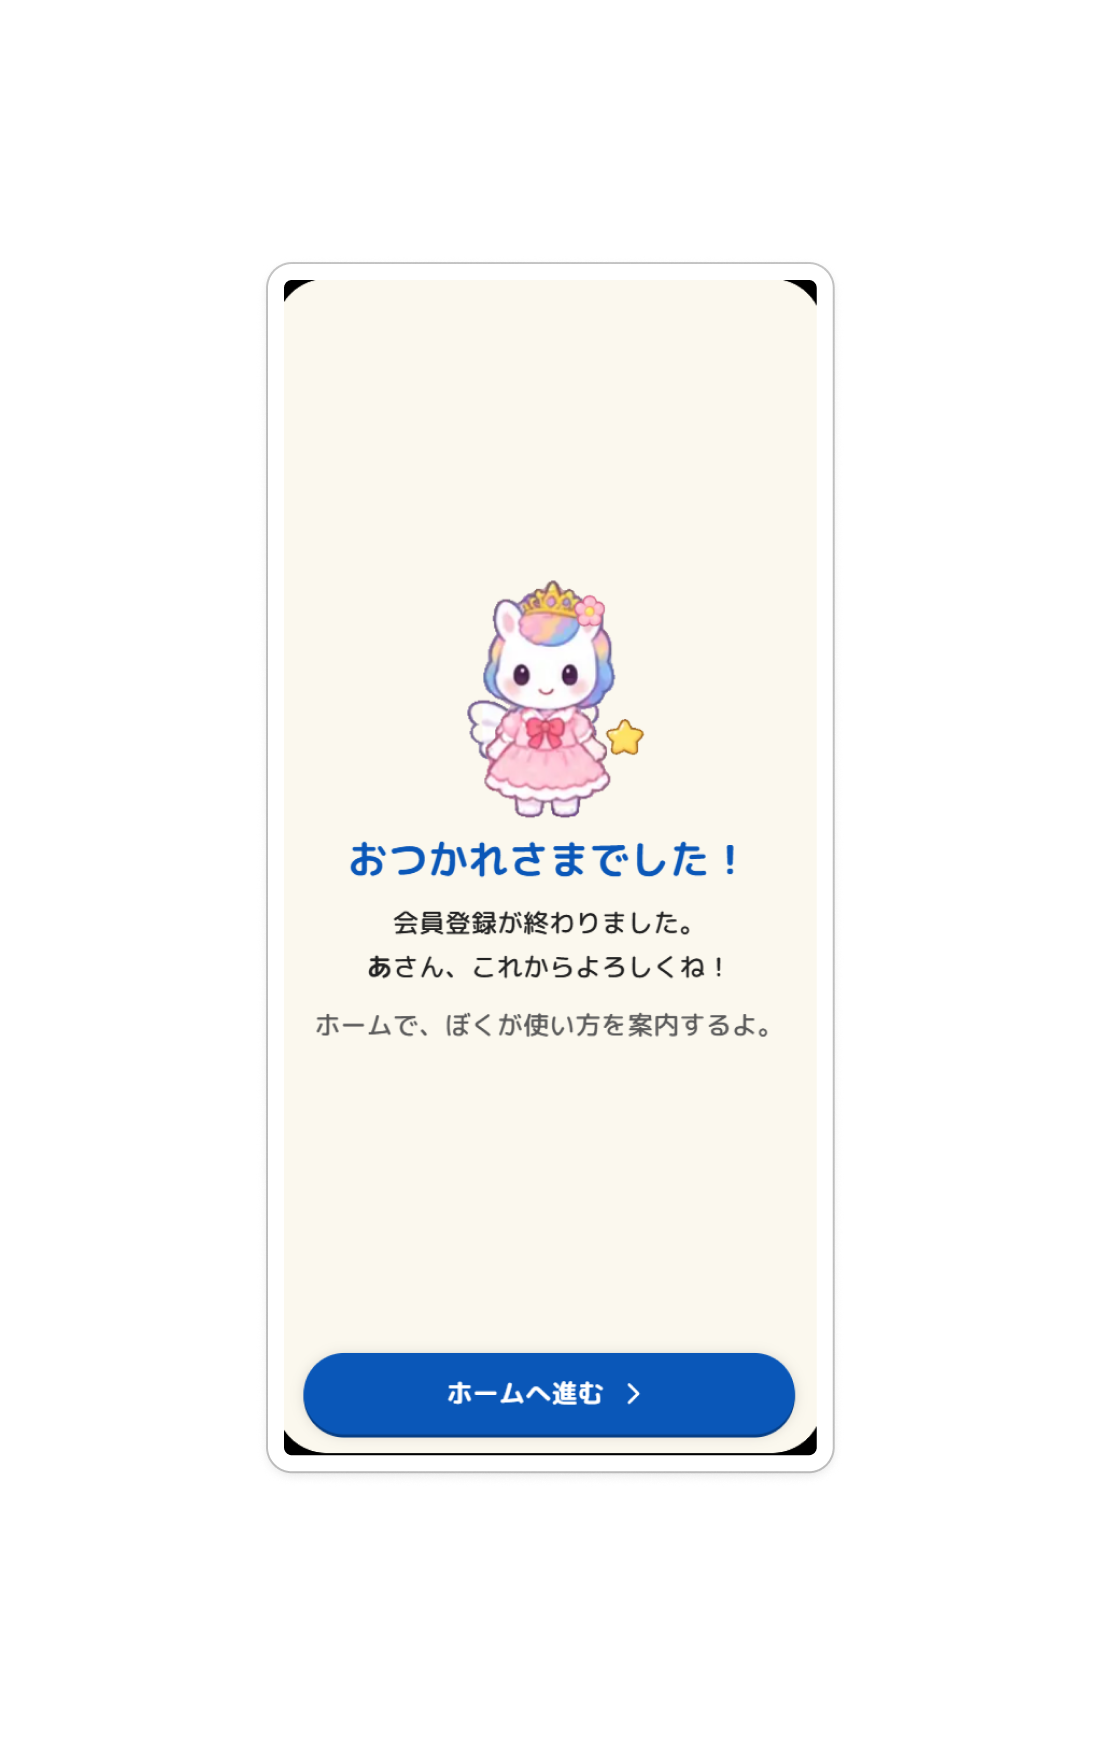
\includegraphics[width=\linewidth]{chapters/images/UI_Screen/reg7.png}
    \caption{登録完了画面}
    \label{fig:reg7}
  \end{subfigure}

  \caption{会員登録画面}
  \label{fig:reg}
\end{figure}

図\ref{fig:reg1}は、学習者の名前（フルネーム）とニックネームを回答する画面である。名前は非公開であり、ニックネームはアプリ内で公開される。

図\ref{fig:reg2}は、学習者の性別を入力する画面である。

図\ref{fig:reg3}は、学習者の生年月日を回答する画面である。上下のボタンをタップ、もしくはスクロールによって数値を変更できる。

図\ref{fig:reg4}は、SMS認証を行うために、電話番号を入力しショートメッセージを送信する画面である。

図\ref{fig:reg5}は、SMSで受信した認証コードを入力し、SMS認証を完了させる画面である。

図\ref{fig:reg6}は、アプリ内でログイン用のパスワードが発行される画面である。利用者は発行されたパスワードを手元に保存し、確認のチェックボックスにチェックを入れる。

図\ref{fig:reg7}は、会員登録完了の画面である。「ホームへ進む」をタップすると、学習者ホーム画面へ遷移する。


% =================================
\subsubsection{ログイン画面}
% =================================

ログイン画面では、電話番号とパスワードを入力し、SMS認証を行い3ステップでログインを行う。

\begin{figure}[H]
  \centering

  \begin{subfigure}[t]{0.31\linewidth}
    \centering
    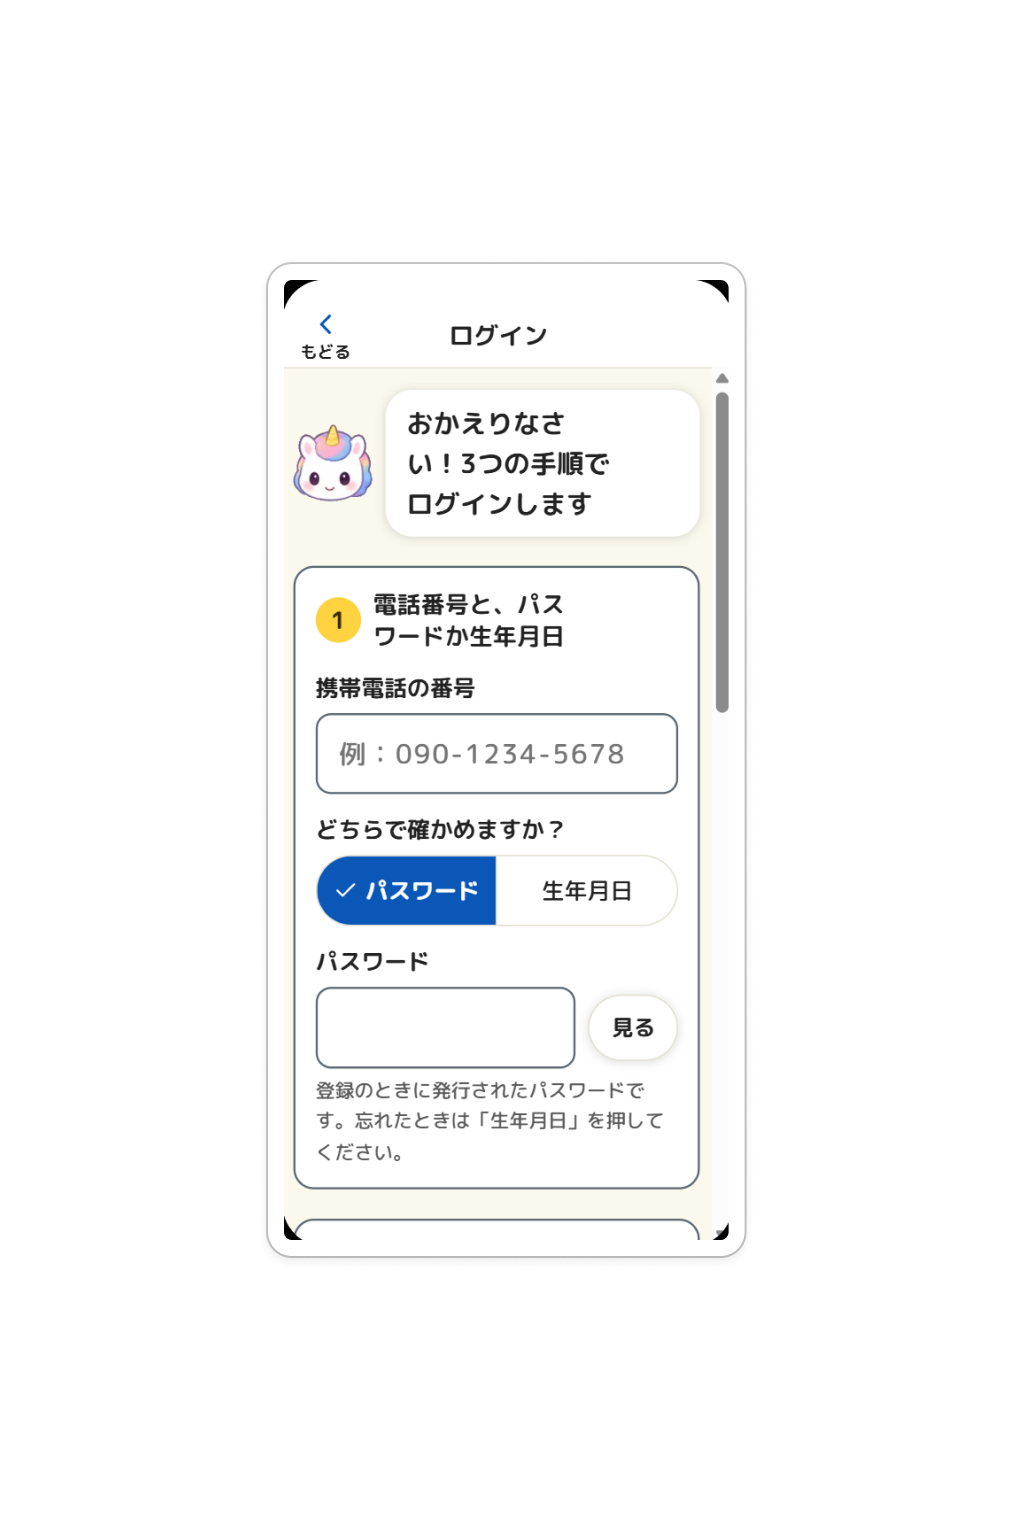
\includegraphics[width=\linewidth]{chapters/images/UI_Screen/rog1.png}
    \caption{ログイン情報入力画面}
    \label{fig:rog1}
  \end{subfigure}
  \hfill
  \begin{subfigure}[t]{0.31\linewidth}
    \centering
    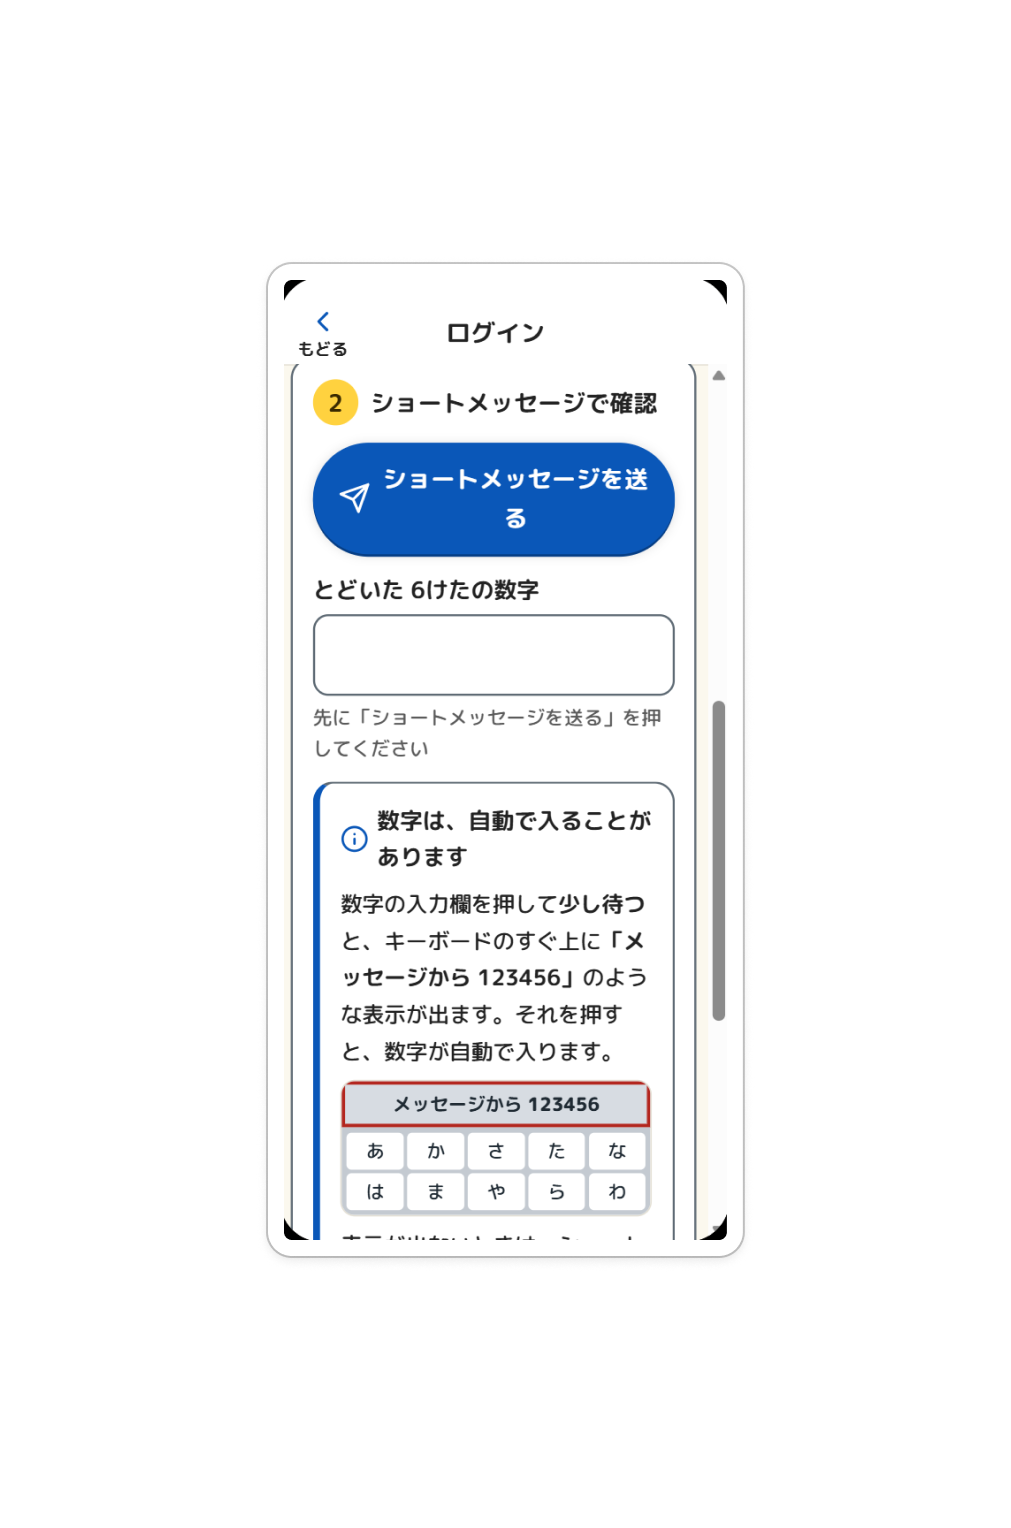
\includegraphics[width=\linewidth]{chapters/images/UI_Screen/rog2.png}
    \caption{SMS認証画面}
    \label{fig:rog2}
  \end{subfigure}
  \hfill
  \begin{subfigure}[t]{0.31\linewidth}
    \centering
    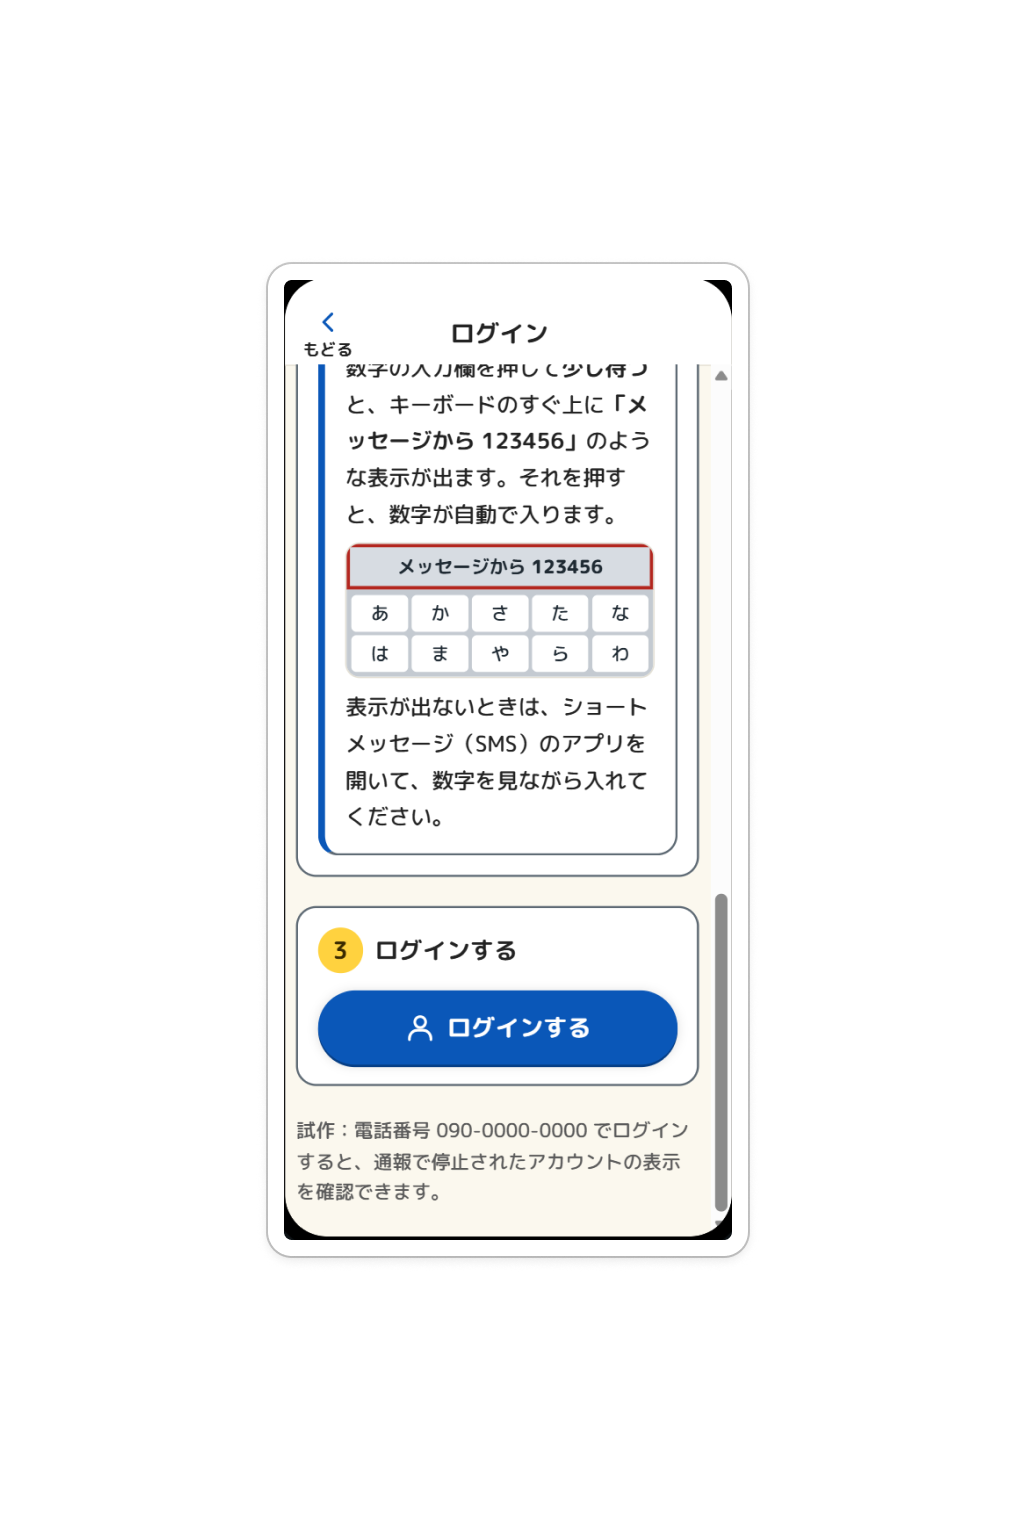
\includegraphics[width=\linewidth]{chapters/images/UI_Screen/rog3.png}
    \caption{ログイン完了画面}
    \label{fig:rog3}
  \end{subfigure}

  \caption{ログイン画面}
  \label{fig:rog}
\end{figure}

図\ref{fig:rog1}は、電話番号とパスワード、もしくは生年月日を入力する画面である。

図\ref{fig:rog2}は、入力した電話番号あてにショートメッセージを送信し、届いた数字を入力する画面である。この際、メッセージの確認方法等の説明を表示する。

図\ref{fig:rog3}は、ログインが完了したことを表示する画面である。


% =================================
\subsubsection{検索画面}
% =================================

図\ref{fig:search1}は、困っていることや操作方法を調べたい内容を検索する画面である。検索バーに任意の形式で入力後、「さがす」をタップすると関連する投稿の一覧画面へ遷移する。また、「カテゴリで調べる」というセクション内のマークをタップすることによって、より曖昧な検索を行うこともできる。最下部には、ほかの学習者が検索している内容を上位5件表示する。

\begin{figure}[H]
  \centering
  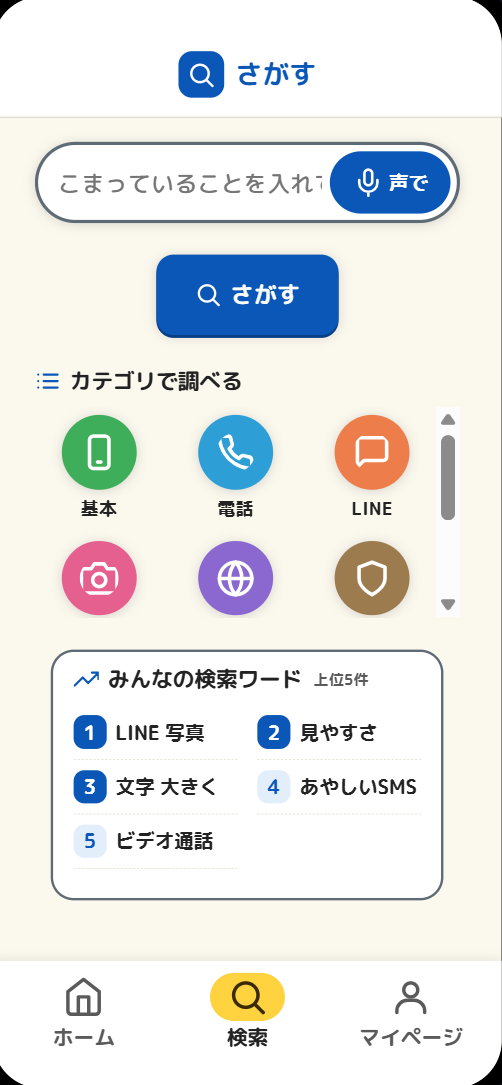
\includegraphics[width=0.55\linewidth]{chapters/images/UI_Screen/serch1.png}
  \caption{検索画面}
  \label{fig:search1}
\end{figure}

図\ref{fig:search2}は、調べた内容に対し関連度順で投稿が表示される画面である。入力された言葉はAIによって分析され、最も関連する投稿を最上部に表示する。また、右下のボタンをタップすると、検索内容と関連する動画が表示されたYouTubeページへ遷移する。

\begin{figure}[H]
  \centering
  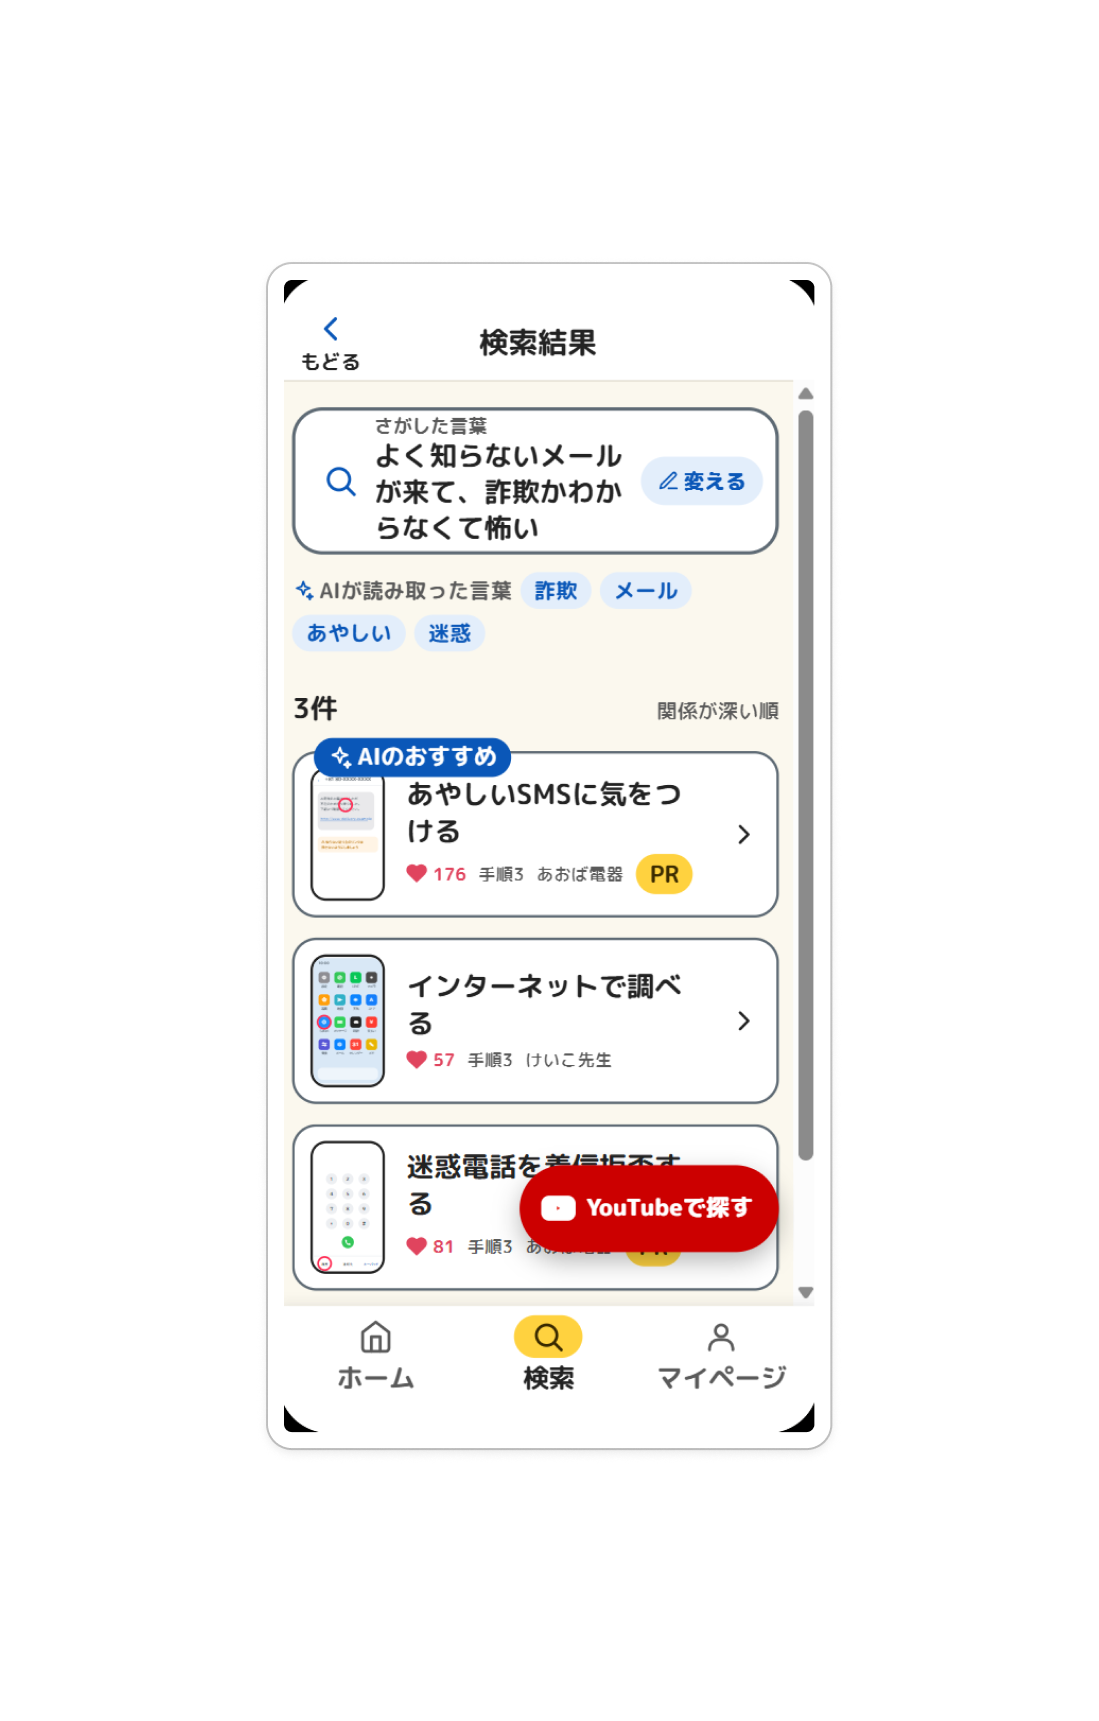
\includegraphics[width=0.55\linewidth]{chapters/images/UI_Screen/serch2.png}
  \caption{投稿一覧画面}
  \label{fig:search2}
\end{figure}

図\ref{fig:search3}は、投稿内容を閲覧する画面である。投稿タイトル、投稿者プロフィール、解説内容が表示される。投稿者プロフィールの右にある手紙をタップすると、投稿者にのみ閲覧可能な個別メッセージを送ることができる。

再生をタップすると音声読み上げを行いながら、自動で解説が進んでいく。また、左右の矢印をタップすることでも次の内容を見ることができる。内容中の青字のリンクをタップすると、用語の解説が表示される。

下部には、いいねを送るリアクションボタン、質問等を入力するコメントボタン、通報を行うためのその他ボタンがある。

\begin{figure}[H]
  \centering
  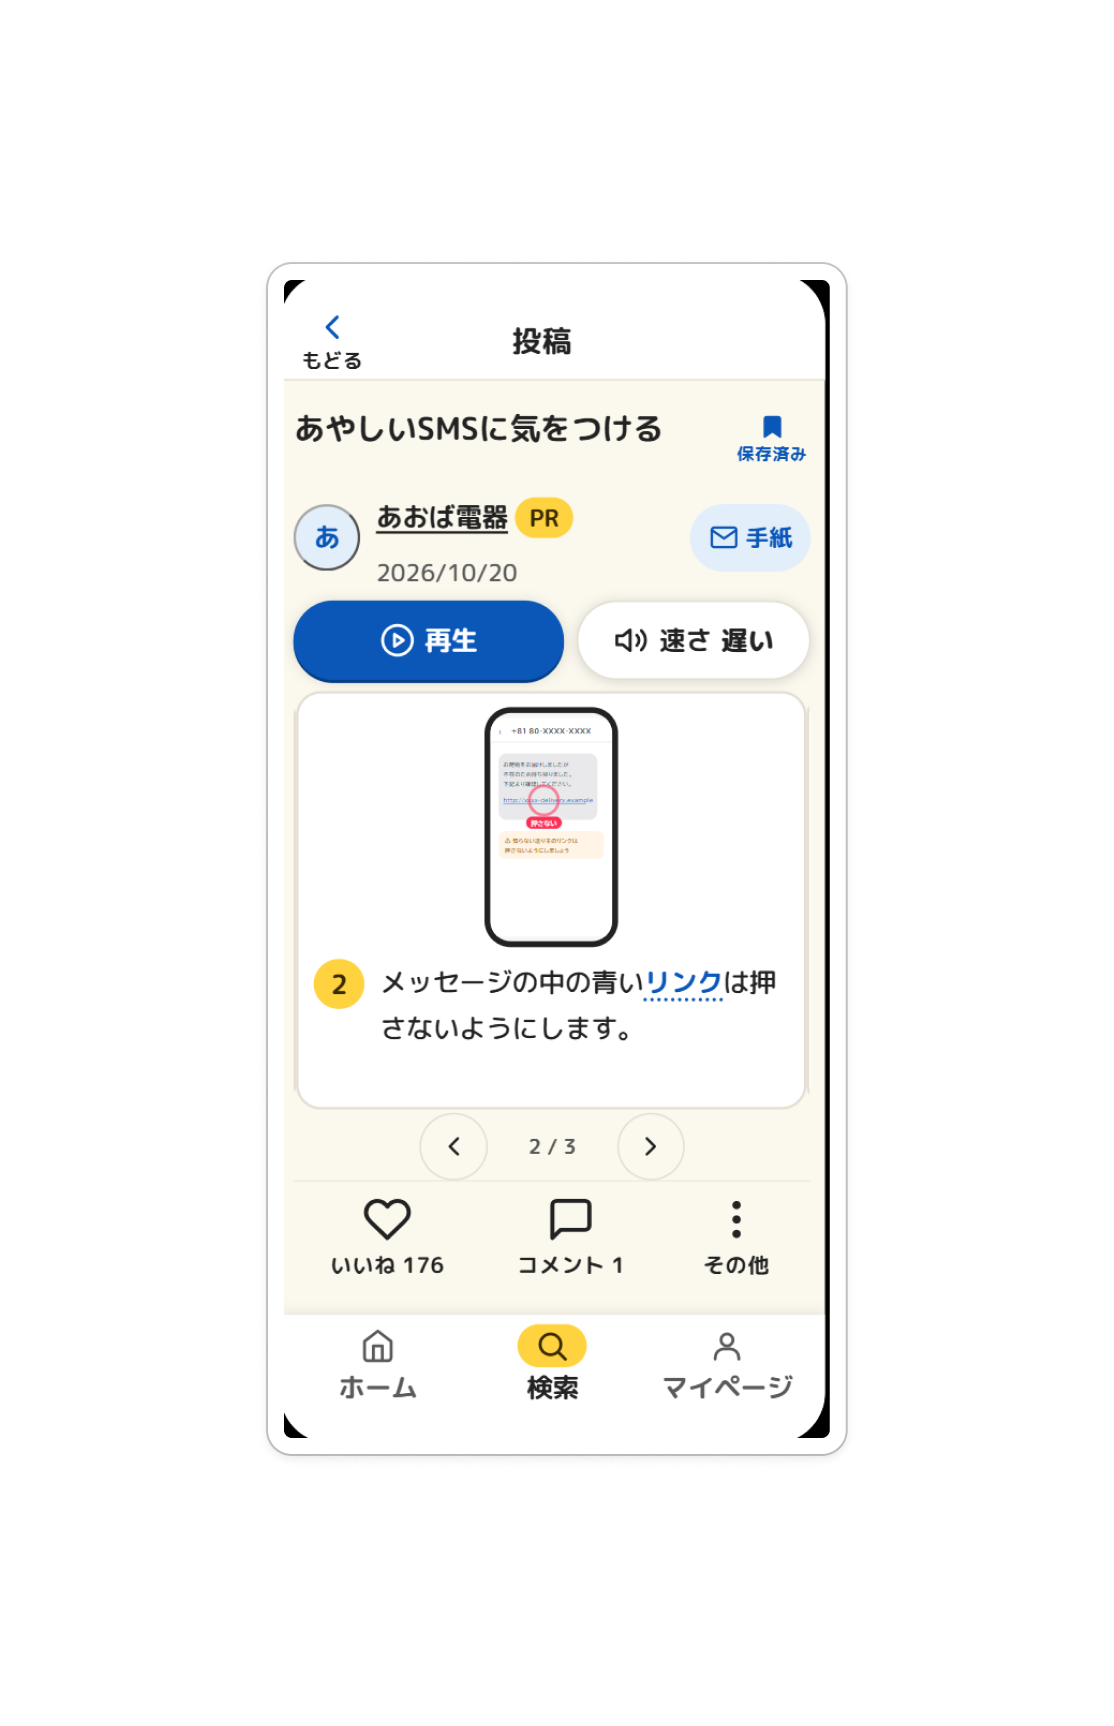
\includegraphics[width=0.55\linewidth]{chapters/images/UI_Screen/serch3.png}
  \caption{投稿閲覧画面}
  \label{fig:search3}
\end{figure}


% =================================
\subsection{学習者画面}
% =================================

\subsubsection{ナビゲーション}

以下に、学習者画面に表示されるナビゲーション画面を示す。

図\ref{fig:navi_top}は、画面の上部に表示されるナビゲーションバーである。アプリのロゴが表示され、その横にヘルプ、お知らせ、設定へ遷移するボタンが配置される。

図\ref{fig:navi_bottom}は、画面の下部に表示されるナビゲーションバーである。ホーム、検索、マイページの3つの遷移ボタンが配置され、現在開いているページはわかりやすくカラー付けされる。

\begin{figure}[H]
  \centering

  \begin{subfigure}[t]{0.45\linewidth}
    \centering
    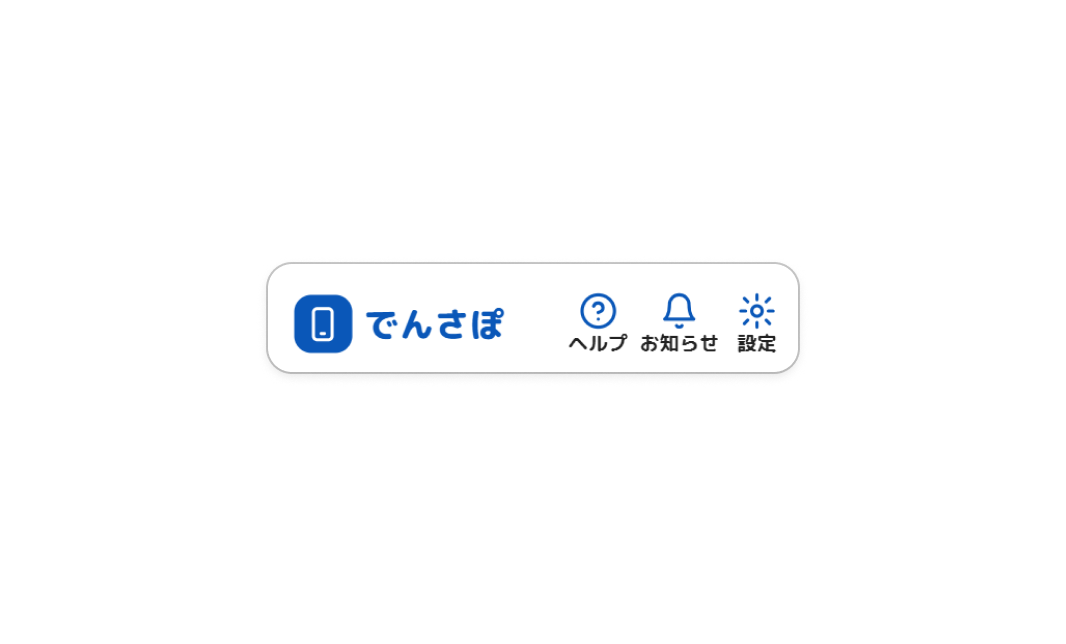
\includegraphics[width=\linewidth]{chapters/images/UI_Screen/lerner/navi_top.png}
    \caption{上部ナビゲーション}
    \label{fig:navi_top}
  \end{subfigure}
  \hfill
  \begin{subfigure}[t]{0.45\linewidth}
    \centering
    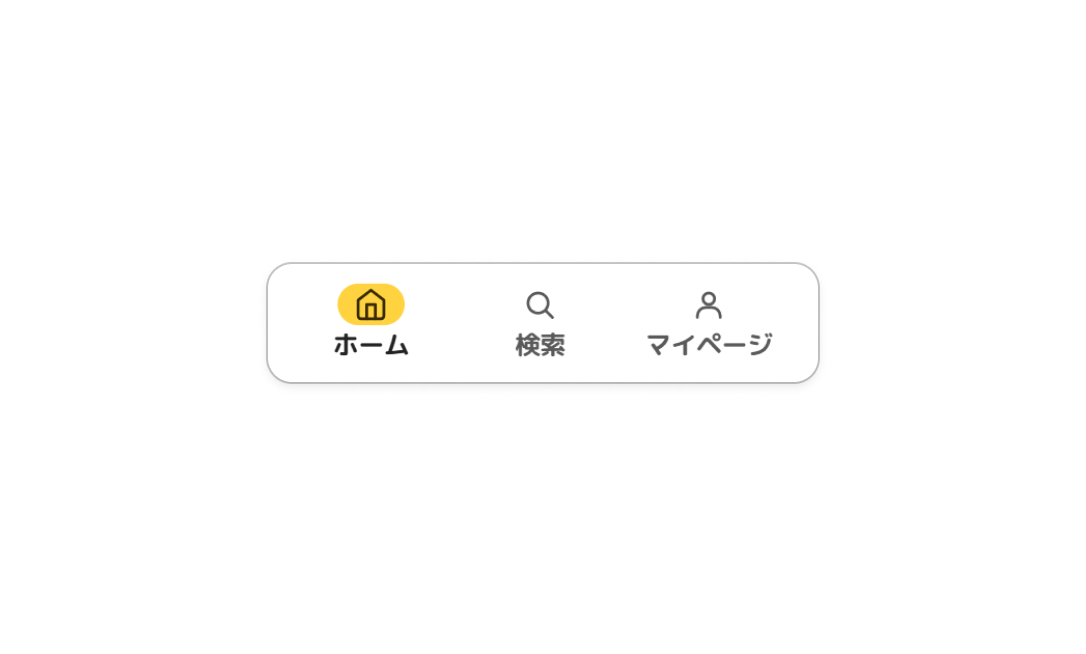
\includegraphics[width=\linewidth]{chapters/images/UI_Screen/lerner/navi_bottom.png}
    \caption{下部ナビゲーション}
    \label{fig:navi_bottom}
  \end{subfigure}

  \caption{ナビゲーション画面}
  \label{fig:navi}
\end{figure}


\subsubsection{ホーム画面}

図\ref{fig:home}は、学習者のホーム画面である。初回起動時はアプリのチュートリアルが表示される。キャラクターをタップすると吹き出し内の一言が変化する。情報・イベント欄にはカテゴリ別に追加されたイベント情報やタイアップ広告等が表示される。

\begin{figure}[H]
  \centering
  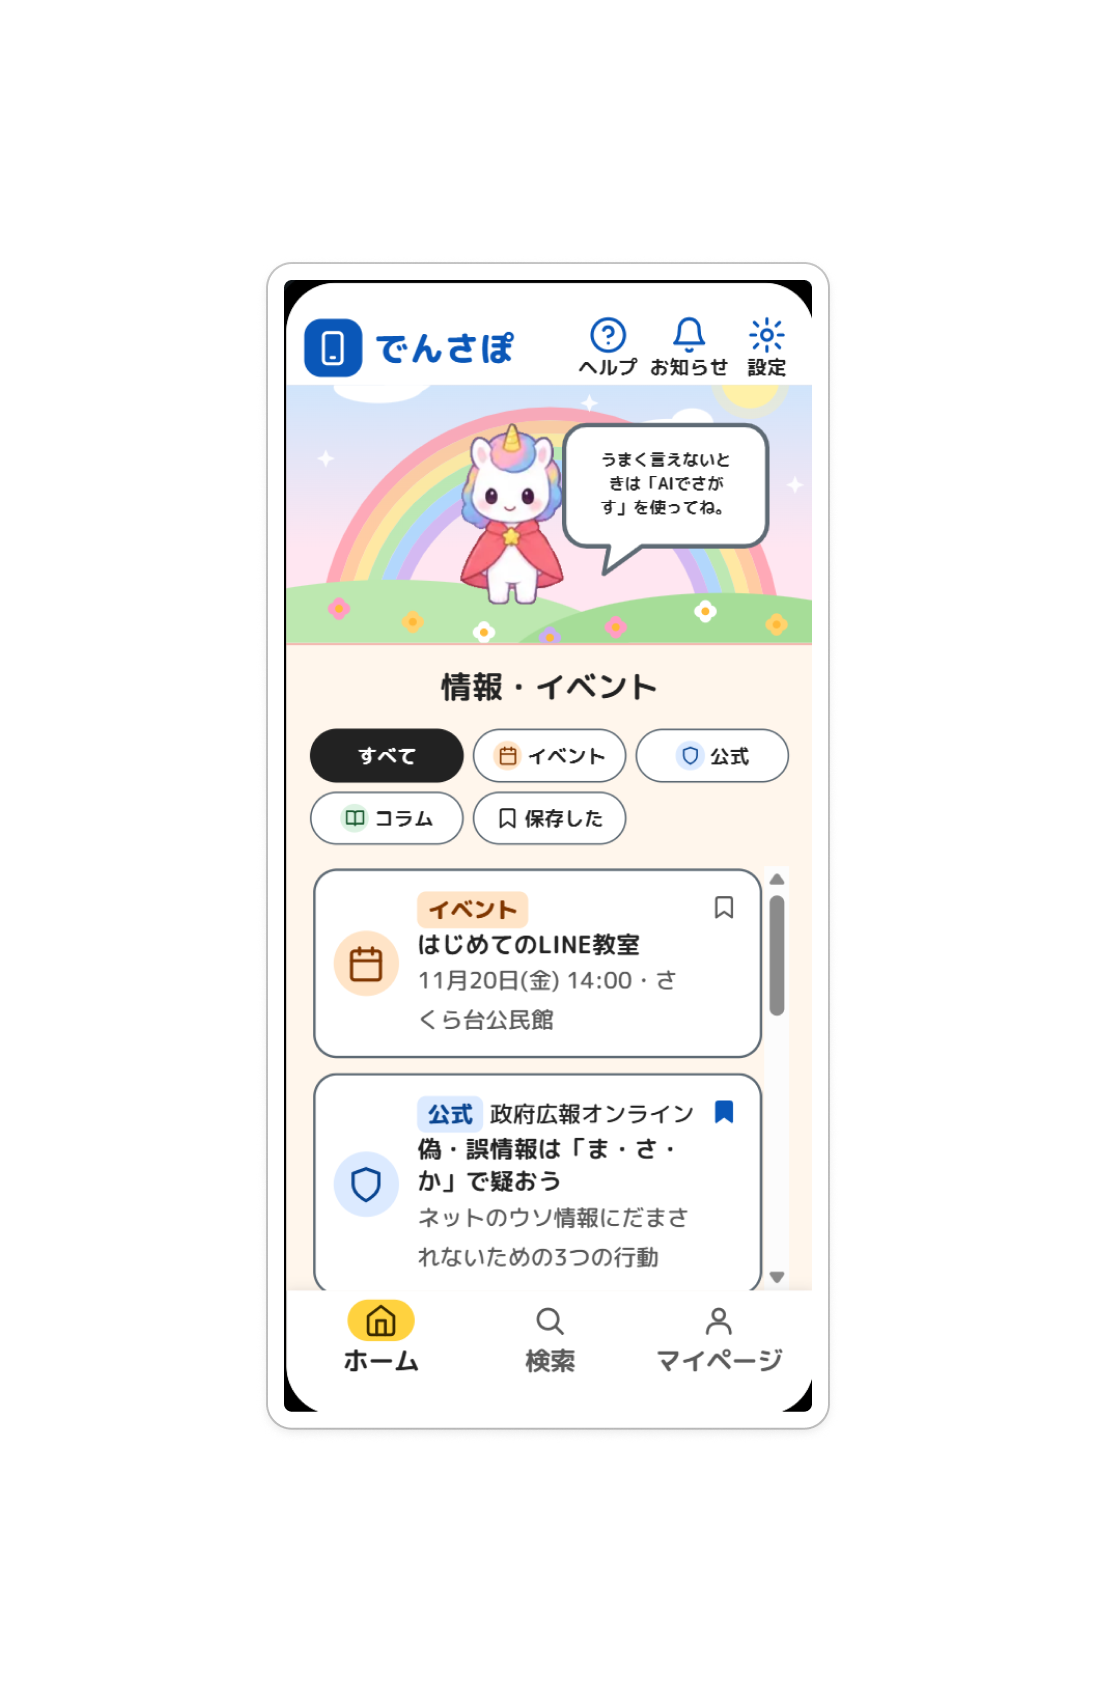
\includegraphics[width=0.55\linewidth]{chapters/images/UI_Screen/lerner/home.png}
  \caption{ホーム画面}
  \label{fig:home}
\end{figure}


\subsubsection{ヘルプ画面}

図\ref{fig:help}は、アプリの使い方等を確認できる画面である。「使い方」をタップすると、チュートリアルを見返すことができる。「よくある質問」では、多くの利用者が問い合わせる内容の回答を確認できる。「お問い合わせ」では、実際に運営側に対して送りたいメッセージを入力して送信することができる。

\begin{figure}[H]
  \centering
  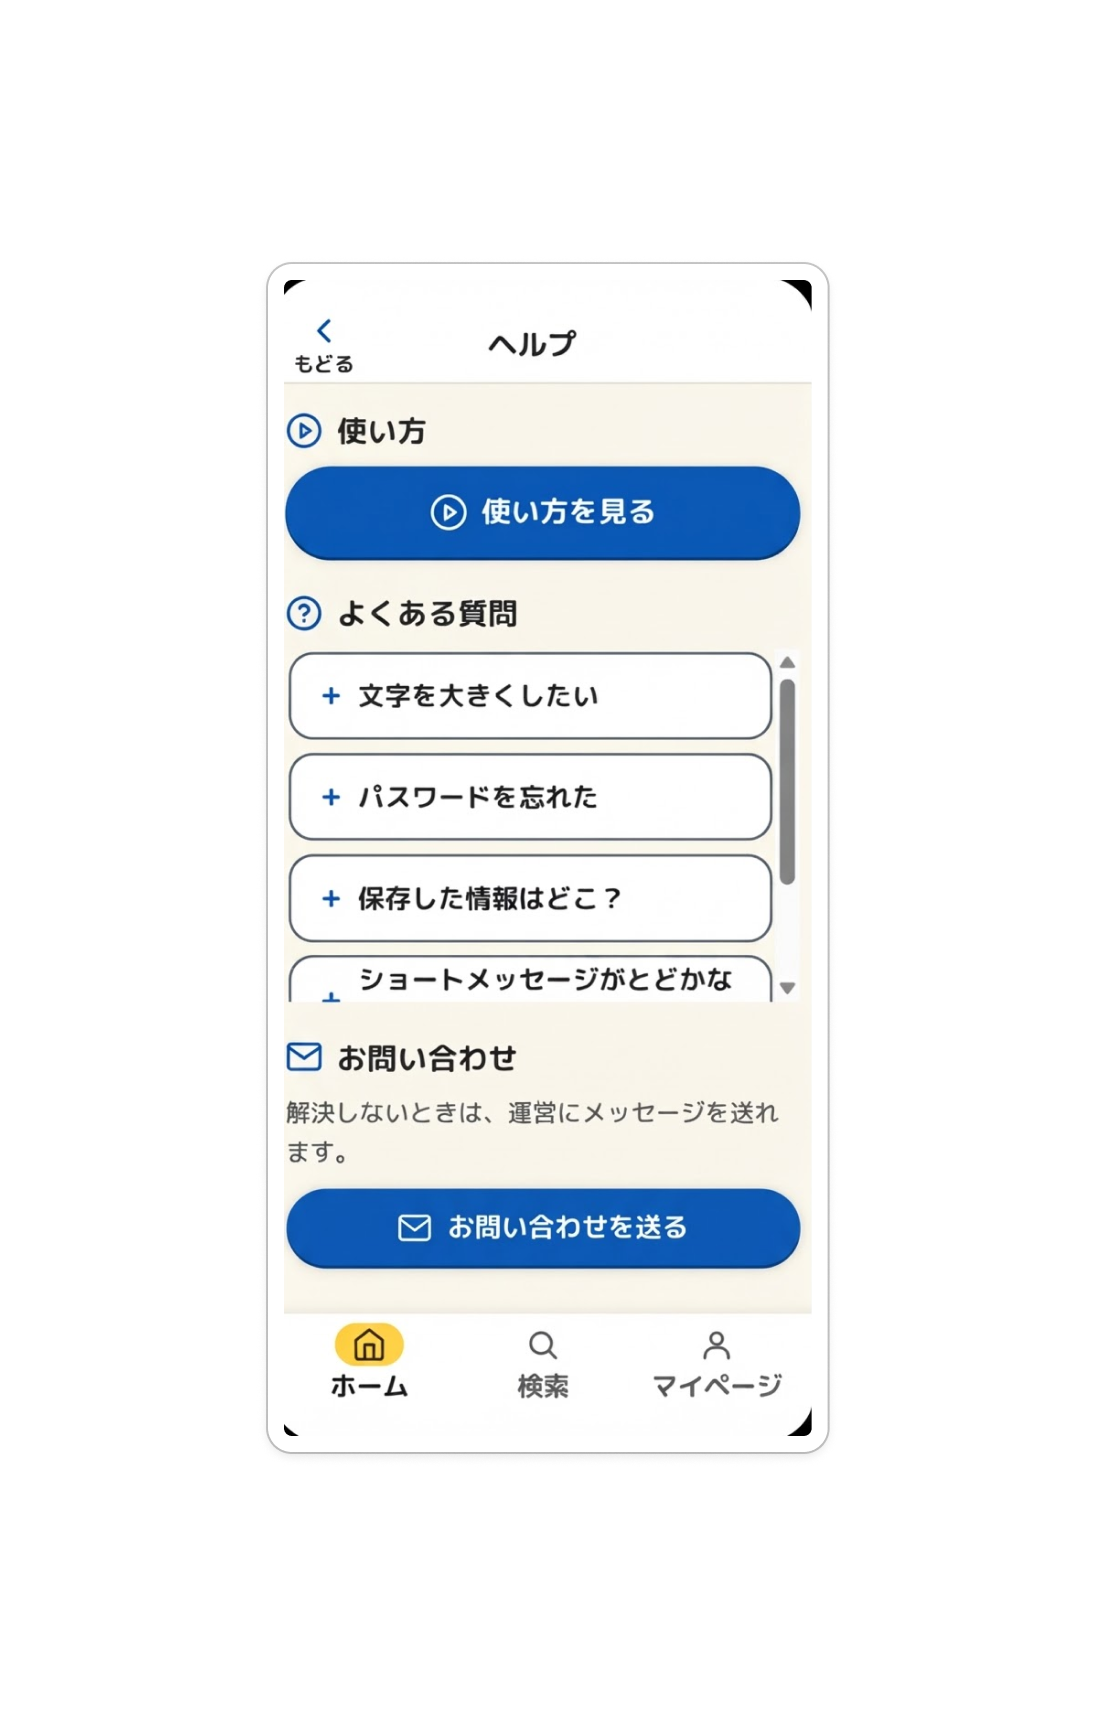
\includegraphics[width=0.55\linewidth]{chapters/images/UI_Screen/lerner/help.png}
  \caption{ヘルプ画面}
  \label{fig:help}
\end{figure}


\subsubsection{設定画面}

図\ref{fig:setting}および図\ref{fig:setting2}は、アプリ内の音量や文字の大きさ、通知設定などを行うことができる画面である。通知設定では受け取る通知の種類を設定することができる。文字の大きさは小・中・大から選択でき、画面の色はホワイトかブラックから選択できる。音量はバーの移動によって設定することができる。

\begin{figure}[H]
  \centering

  \begin{subfigure}[t]{0.45\linewidth}
    \centering
    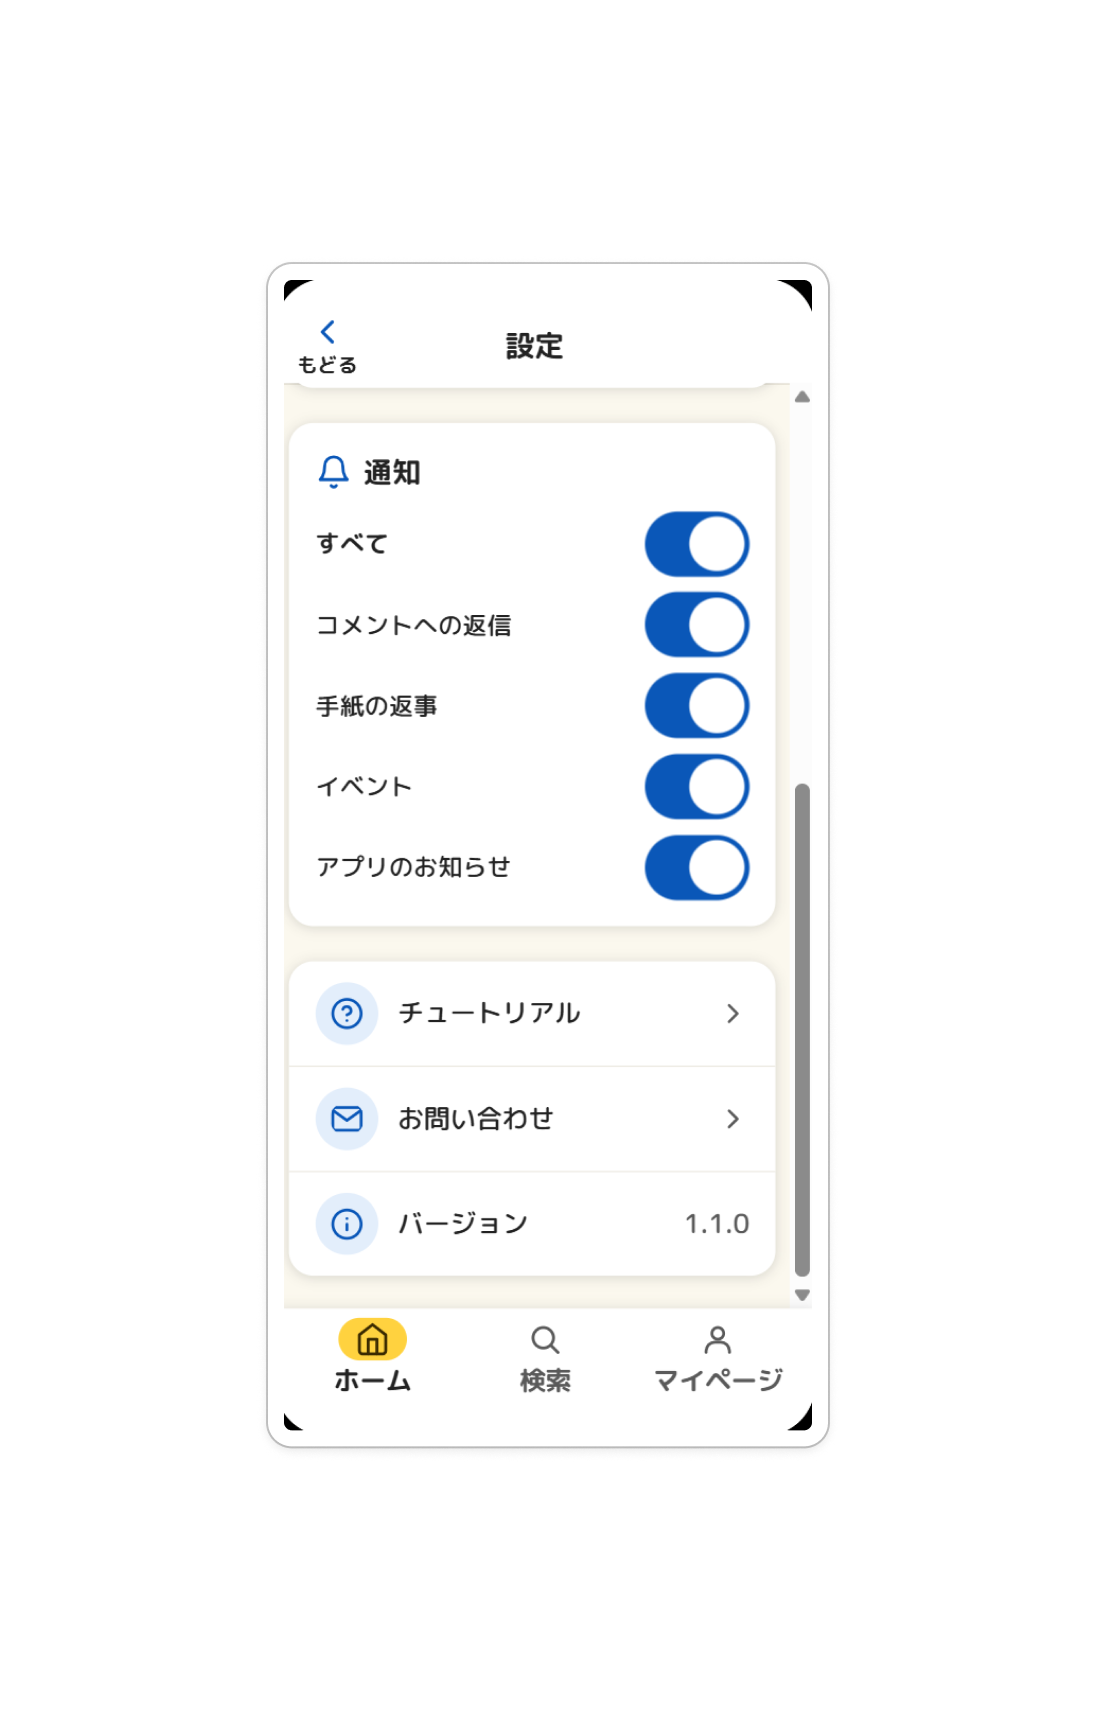
\includegraphics[width=\linewidth]{chapters/images/UI_Screen/lerner/setting.png}
    \caption{設定画面}
    \label{fig:setting}
  \end{subfigure}
  \hfill
  \begin{subfigure}[t]{0.45\linewidth}
    \centering
    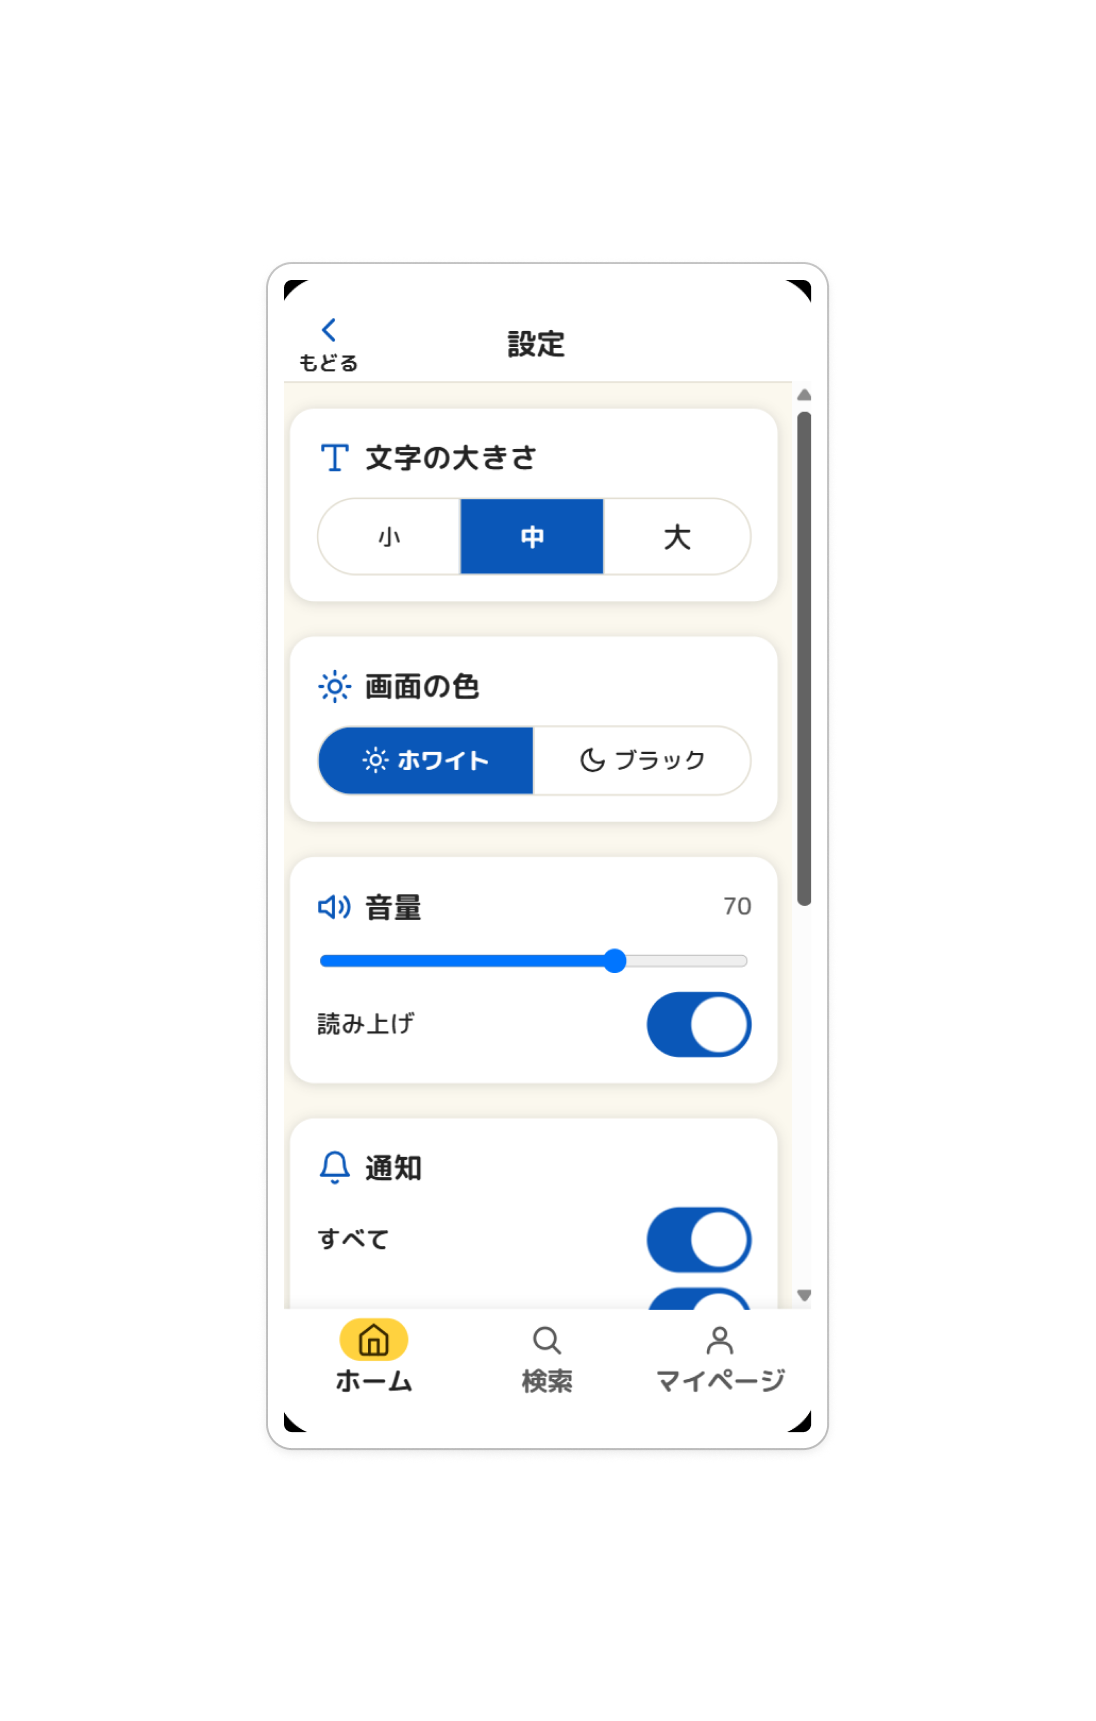
\includegraphics[width=\linewidth]{chapters/images/UI_Screen/lerner/setting2.png}
    \caption{設定画面}
    \label{fig:setting2}
  \end{subfigure}

  \caption{設定画面}
  \label{fig:settings}
\end{figure}


\subsubsection{お知らせ画面}

図\ref{fig:info}は、運営からのお知らせや投稿者からの回答などの通知の一覧を確認できる画面である。

\begin{figure}[H]
  \centering
  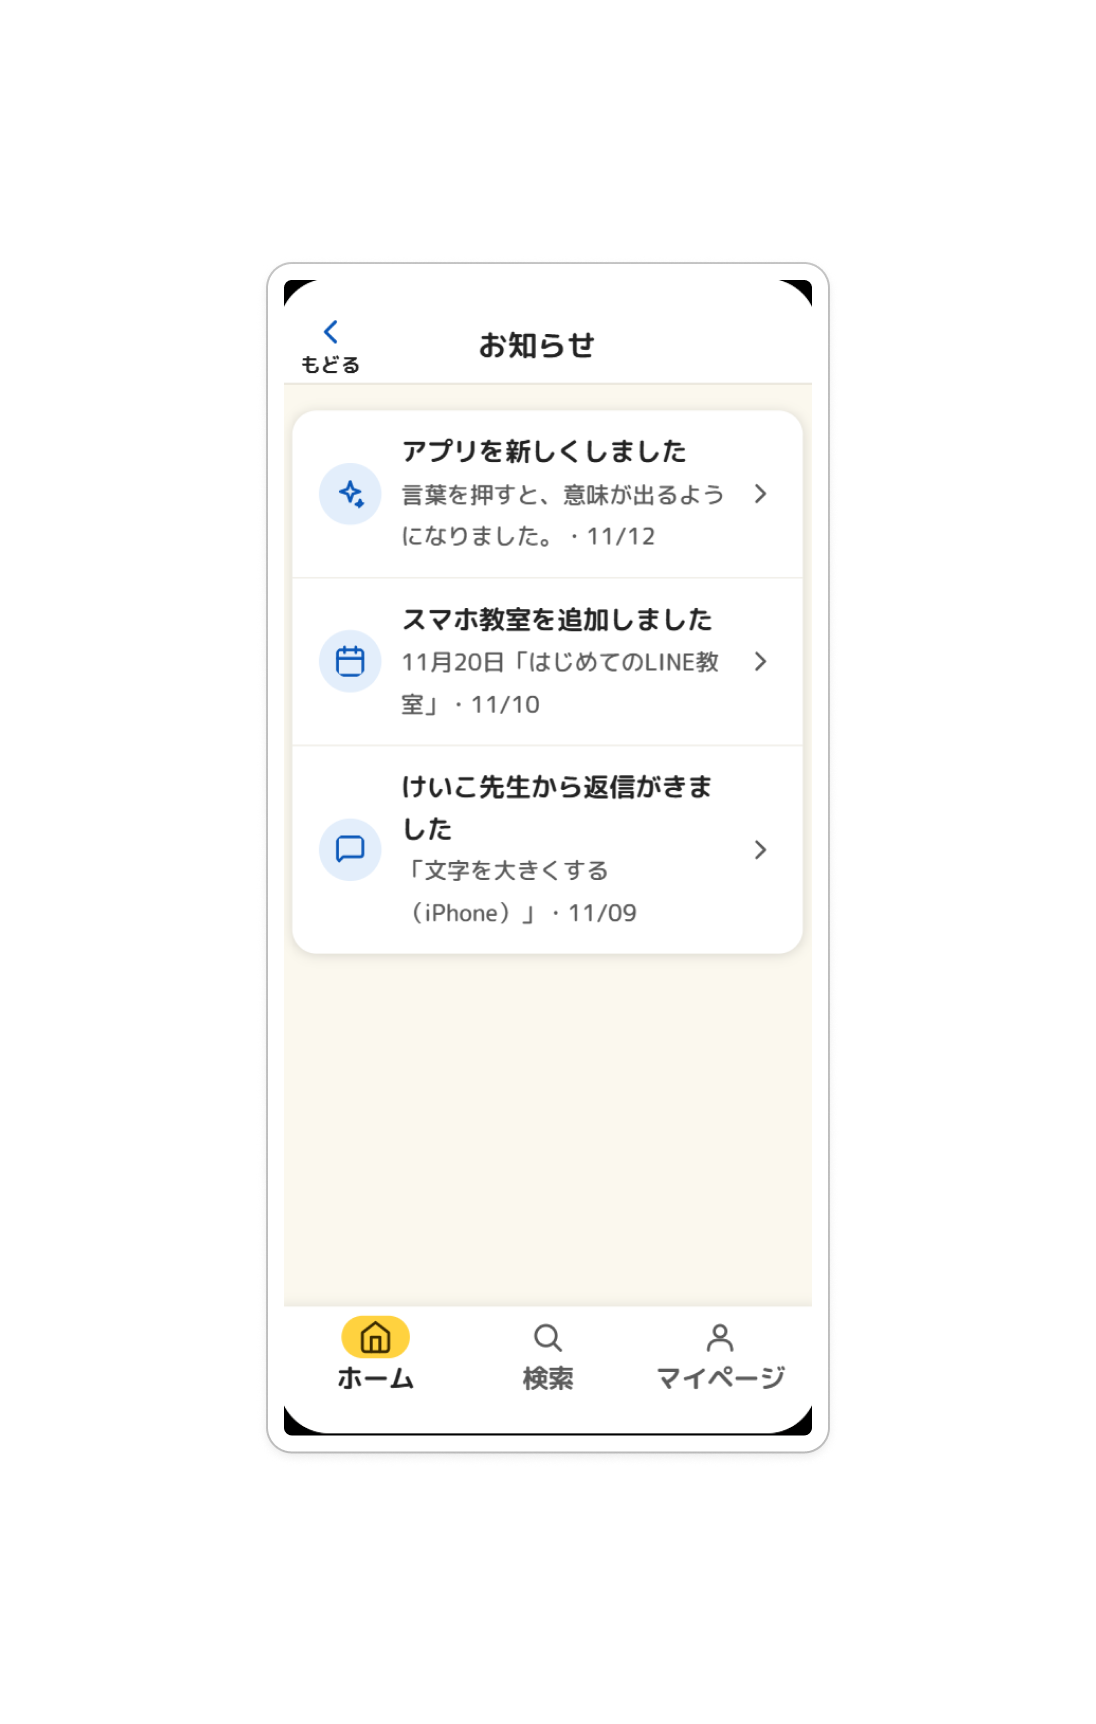
\includegraphics[width=0.55\linewidth]{chapters/images/UI_Screen/lerner/info.png}
  \caption{お知らせ画面}
  \label{fig:info}
\end{figure}


\subsubsection{マイページ画面}

図\ref{fig:mypage}は、ホームに表示されるキャラクターに対する操作や、自分の保存した内容、ミニゲームなど様々な操作を行うことができる画面である。

図\ref{fig:mypage2}は、キャラクター操作欄の表示画面である。着せ替えでは、キャラクターや背景、アクセサリ等をコインを使って購入、変更することができる。行った変更はホームのキャラクター画面に反映される。プロフィールには、アプリ利用開始日などの情報が表示され、鉛筆マークをタップすると編集画面へ遷移する。ミニゲーム、保存したもの、質問の各種ボタンをタップすると、それぞれの画面へ遷移する。

\begin{figure}[H]
  \centering

  \begin{subfigure}[t]{0.45\linewidth}
    \centering
    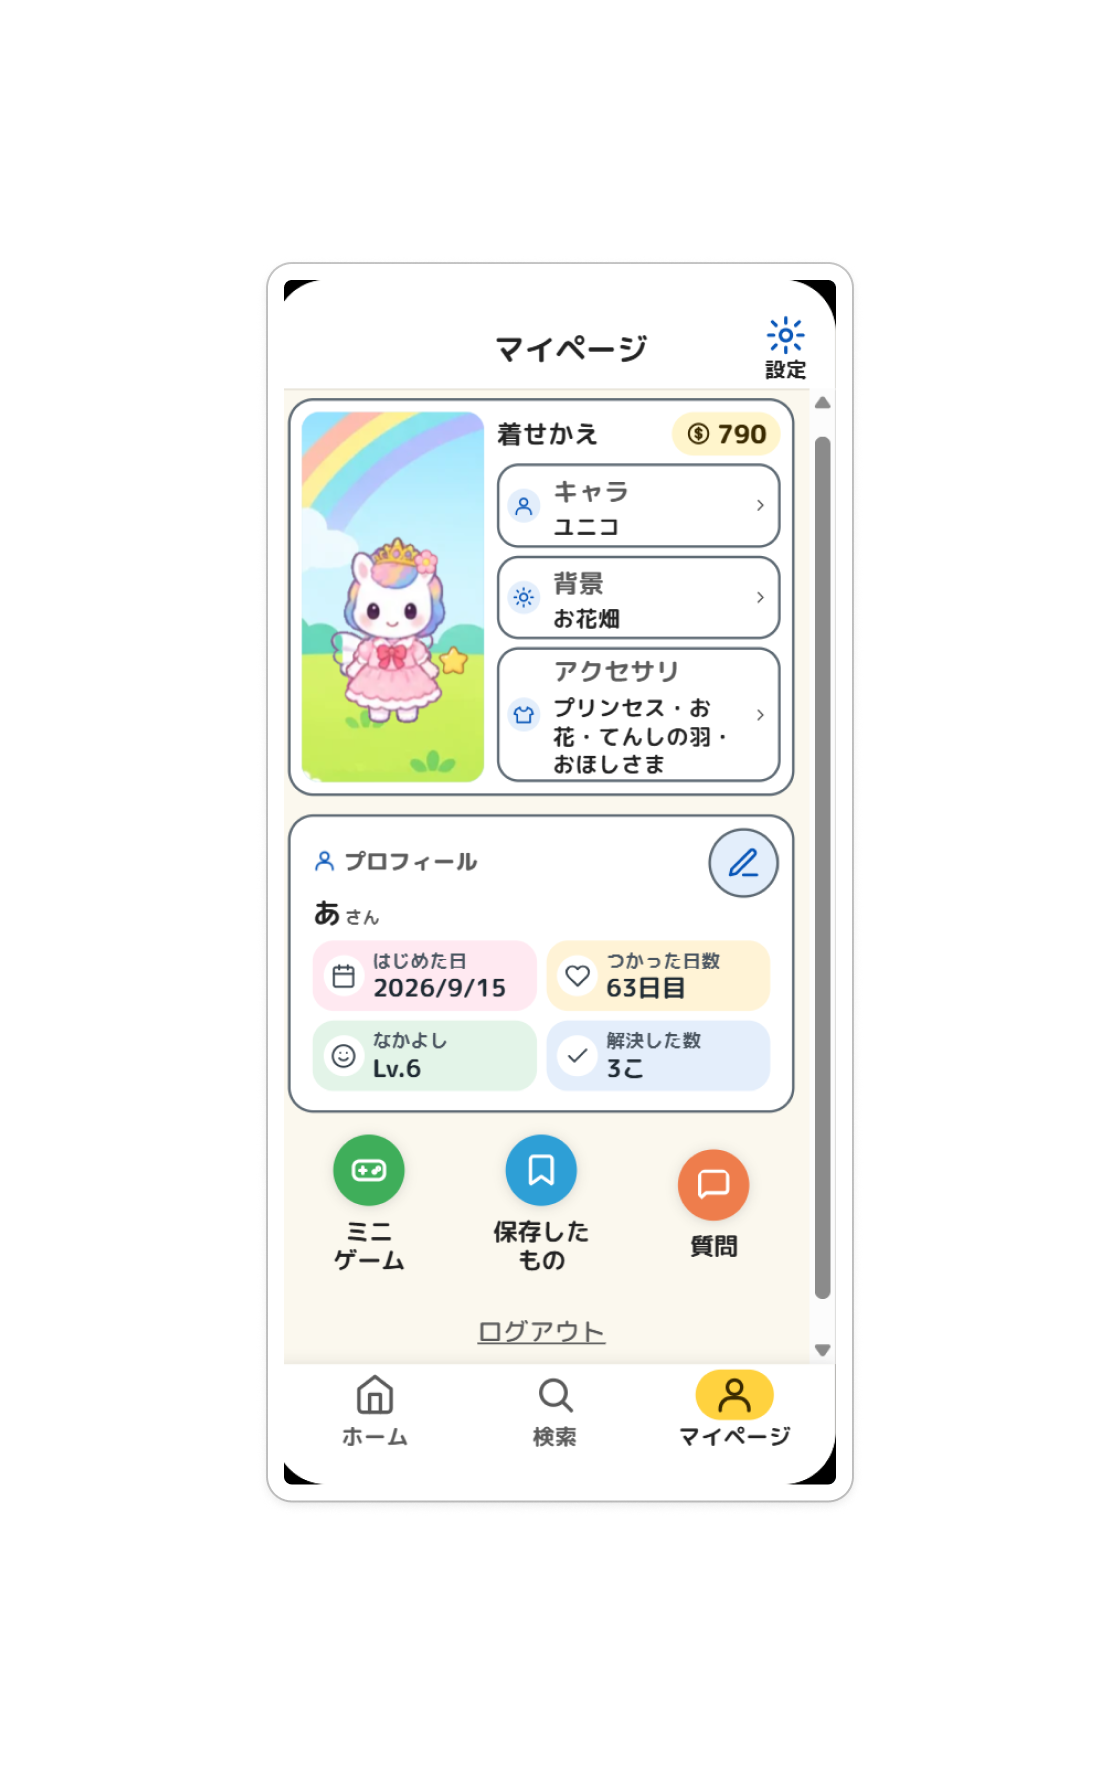
\includegraphics[width=\linewidth]{chapters/images/UI_Screen/lerner/mypage.png}
    \caption{マイページ画面}
    \label{fig:mypage}
  \end{subfigure}
  \hfill
  \begin{subfigure}[t]{0.45\linewidth}
    \centering
    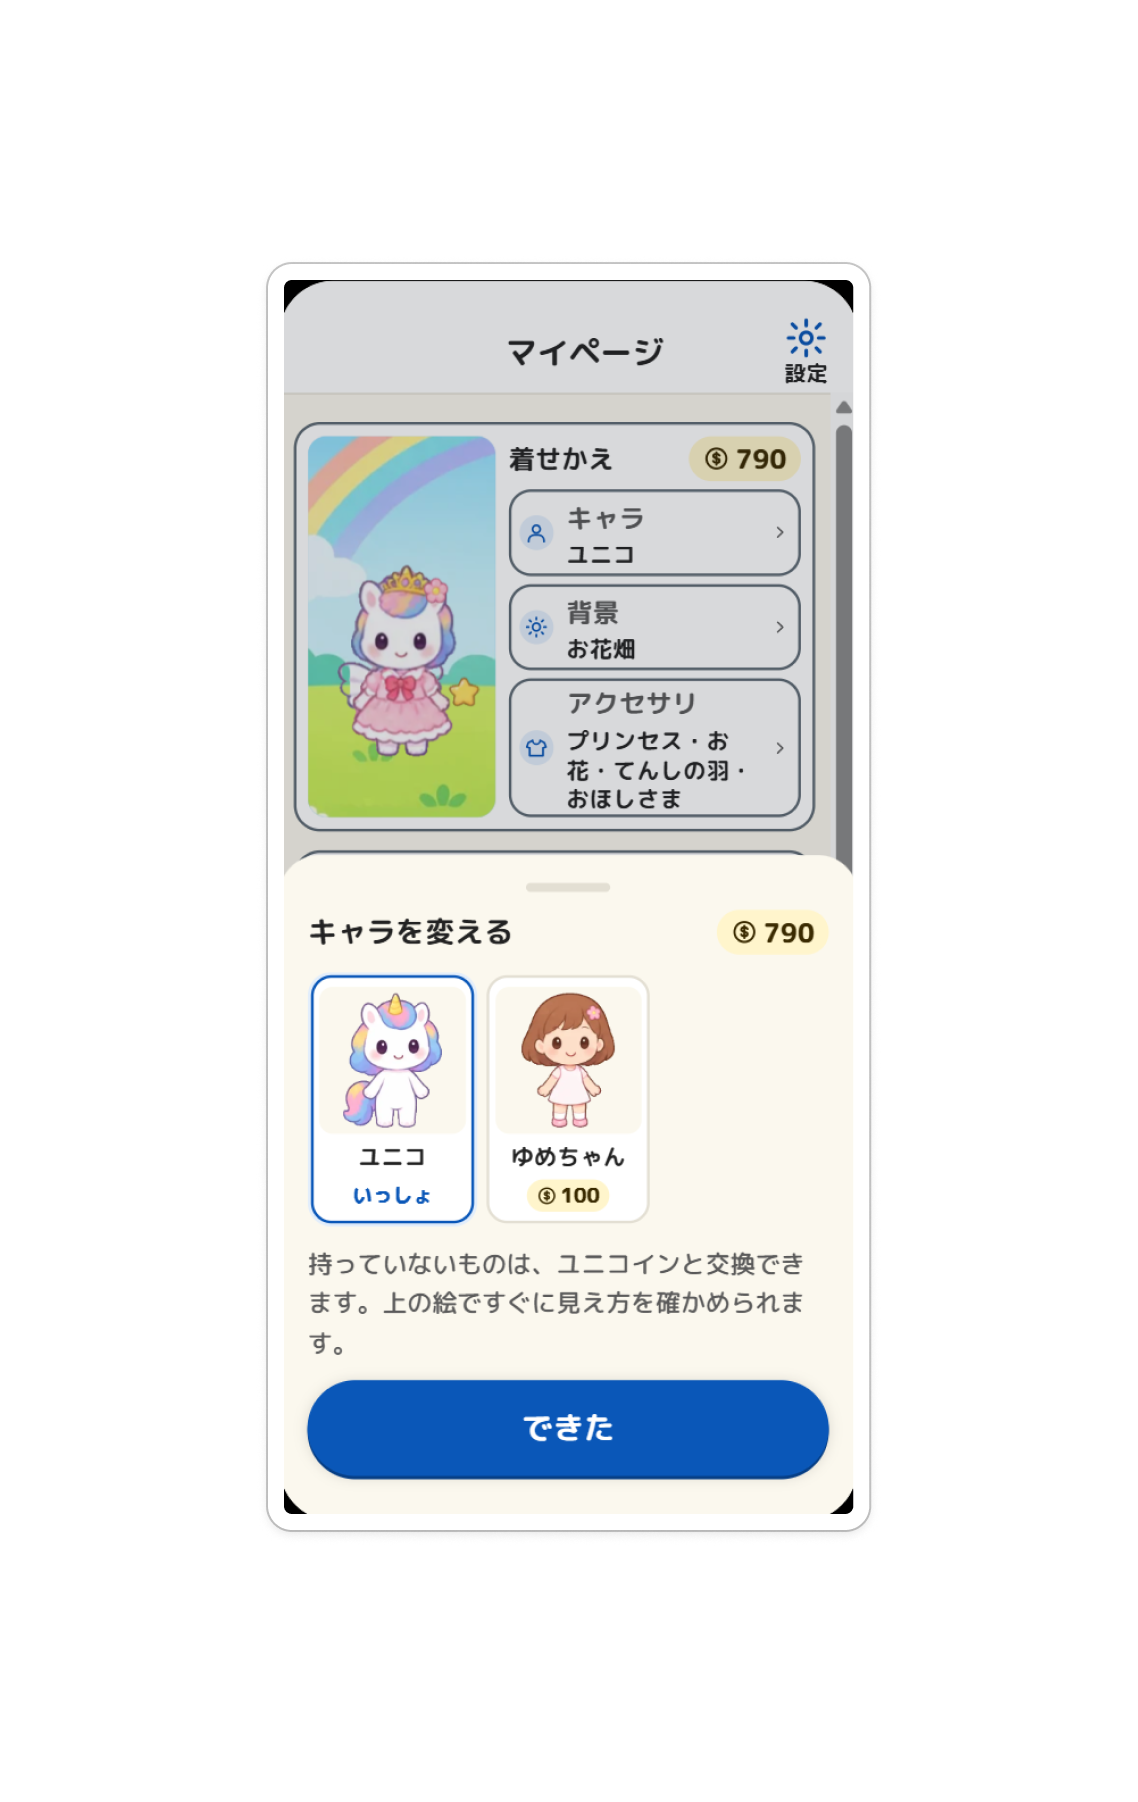
\includegraphics[width=\linewidth]{chapters/images/UI_Screen/lerner/mypage2.png}
    \caption{キャラクター操作欄の表示}
    \label{fig:mypage2}
  \end{subfigure}

  \caption{マイページ画面}
  \label{fig:mypages}
\end{figure}


\subsubsection{プロフィール画面}

図\ref{fig:profile}は、プロフィールの変更を行う画面である。アイコンやニックネーム、パスワードなどの編集を行うことができる。

\begin{figure}[H]
  \centering
  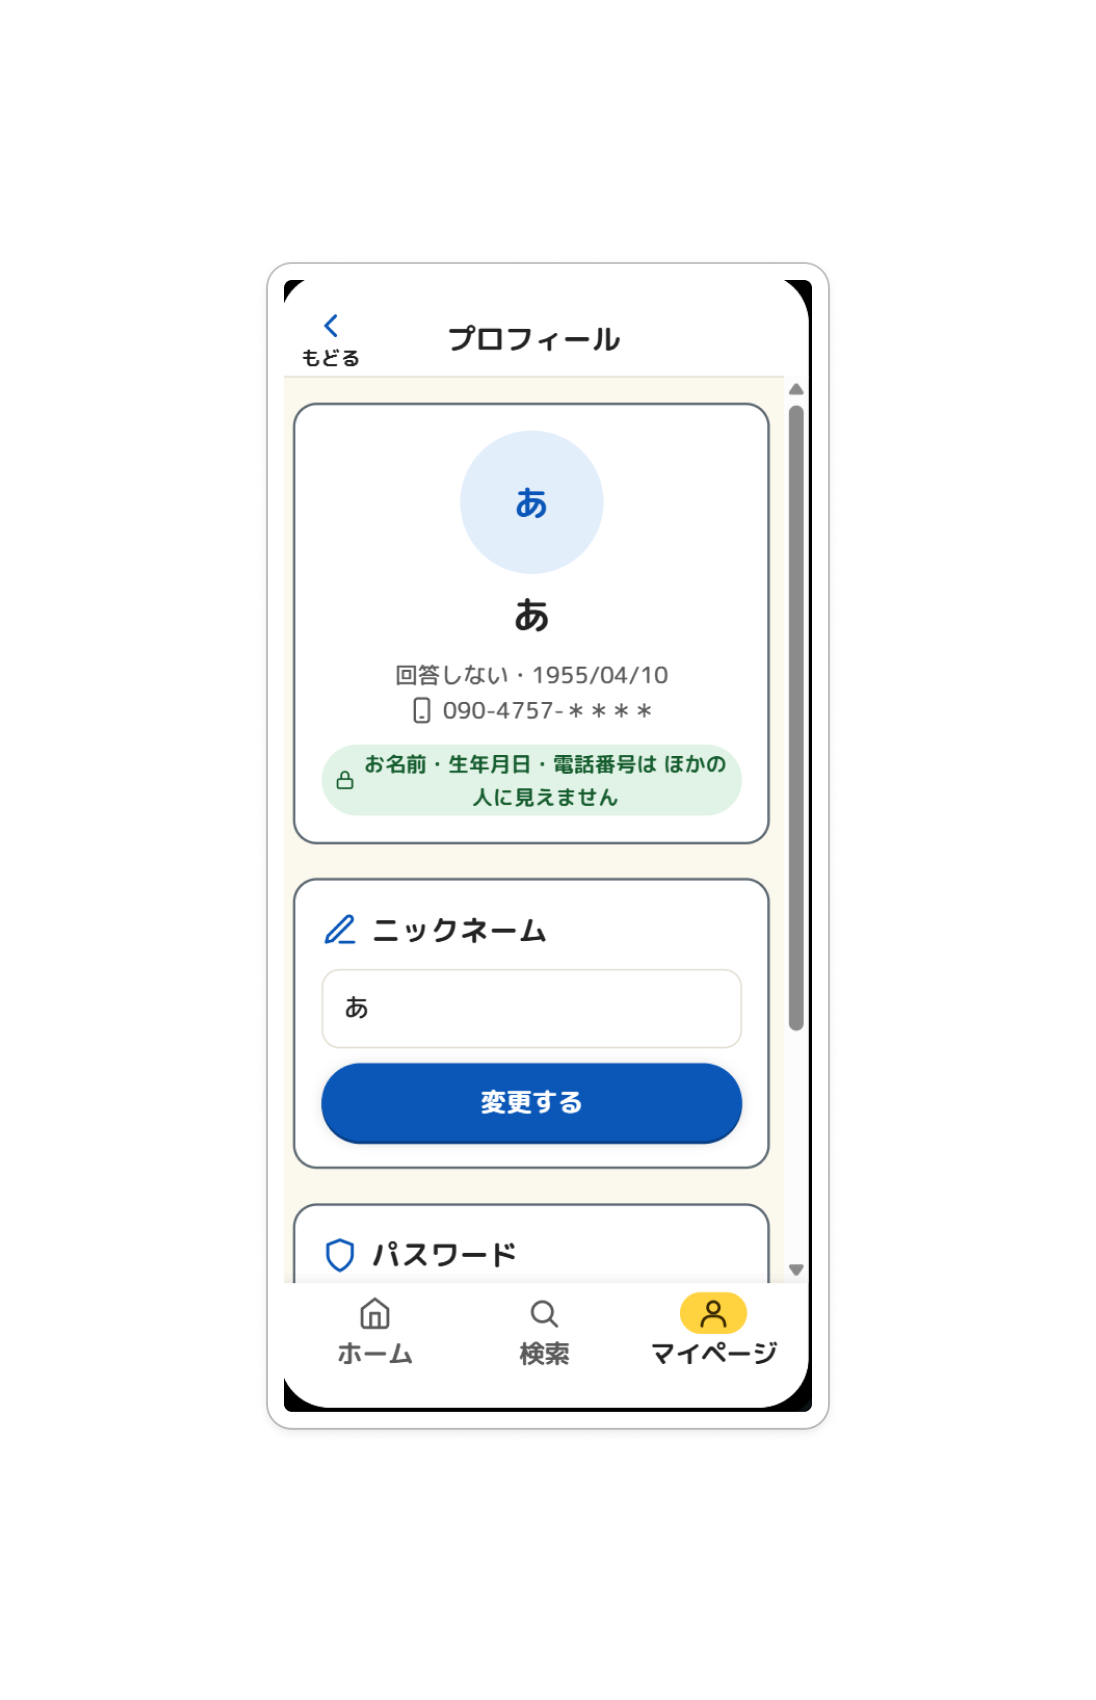
\includegraphics[width=0.55\linewidth]{chapters/images/UI_Screen/lerner/profile.png}
  \caption{プロフィール画面}
  \label{fig:profile}
\end{figure}


\subsubsection{ミニゲーム画面}

図\ref{fig:minigame}は、各種ミニゲームをプレイすることができる画面である。ここでプレイするゲームを選択することができる。未実装ゲームは準備中と表示される。

図\ref{fig:minigame2}は、ミニゲーム「フリック入力」のプレイ画面である。

\begin{figure}[H]
  \centering

  \begin{subfigure}[t]{0.45\linewidth}
    \centering
    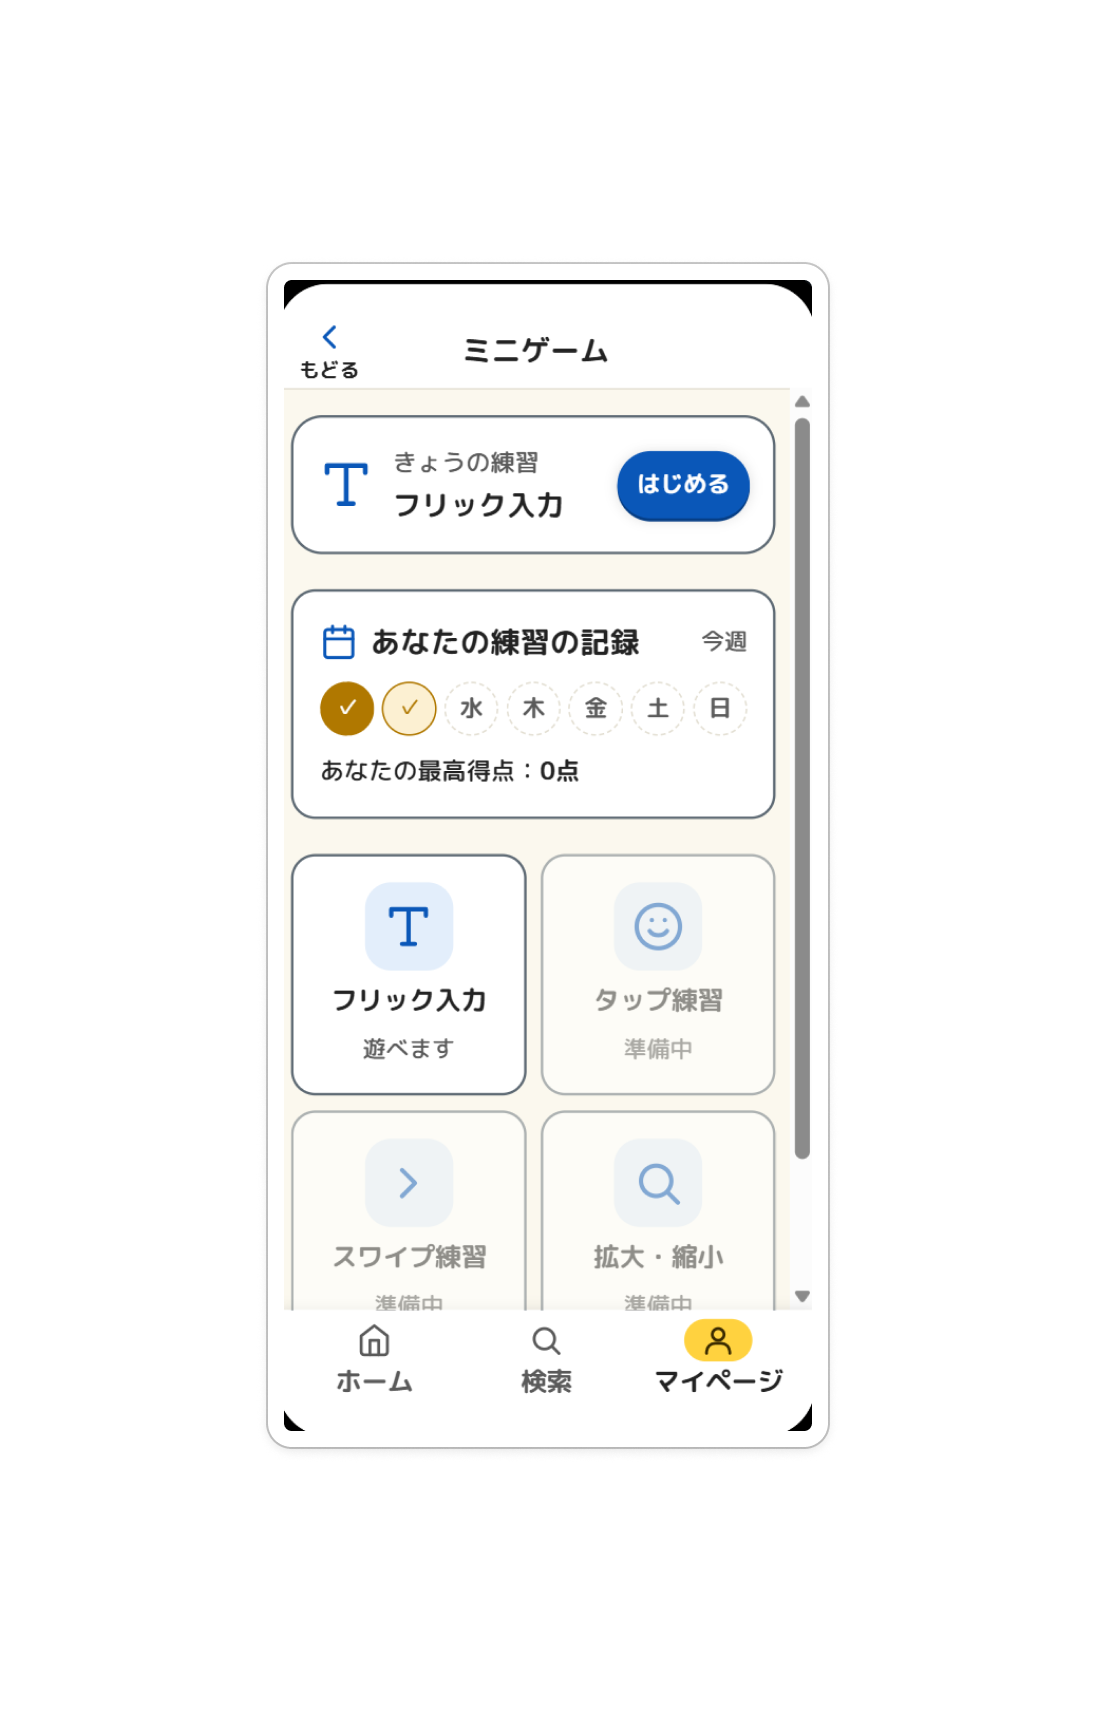
\includegraphics[width=\linewidth]{chapters/images/UI_Screen/lerner/minigame.png}
    \caption{ミニゲーム画面}
    \label{fig:minigame}
  \end{subfigure}
  \hfill
  \begin{subfigure}[t]{0.45\linewidth}
    \centering
    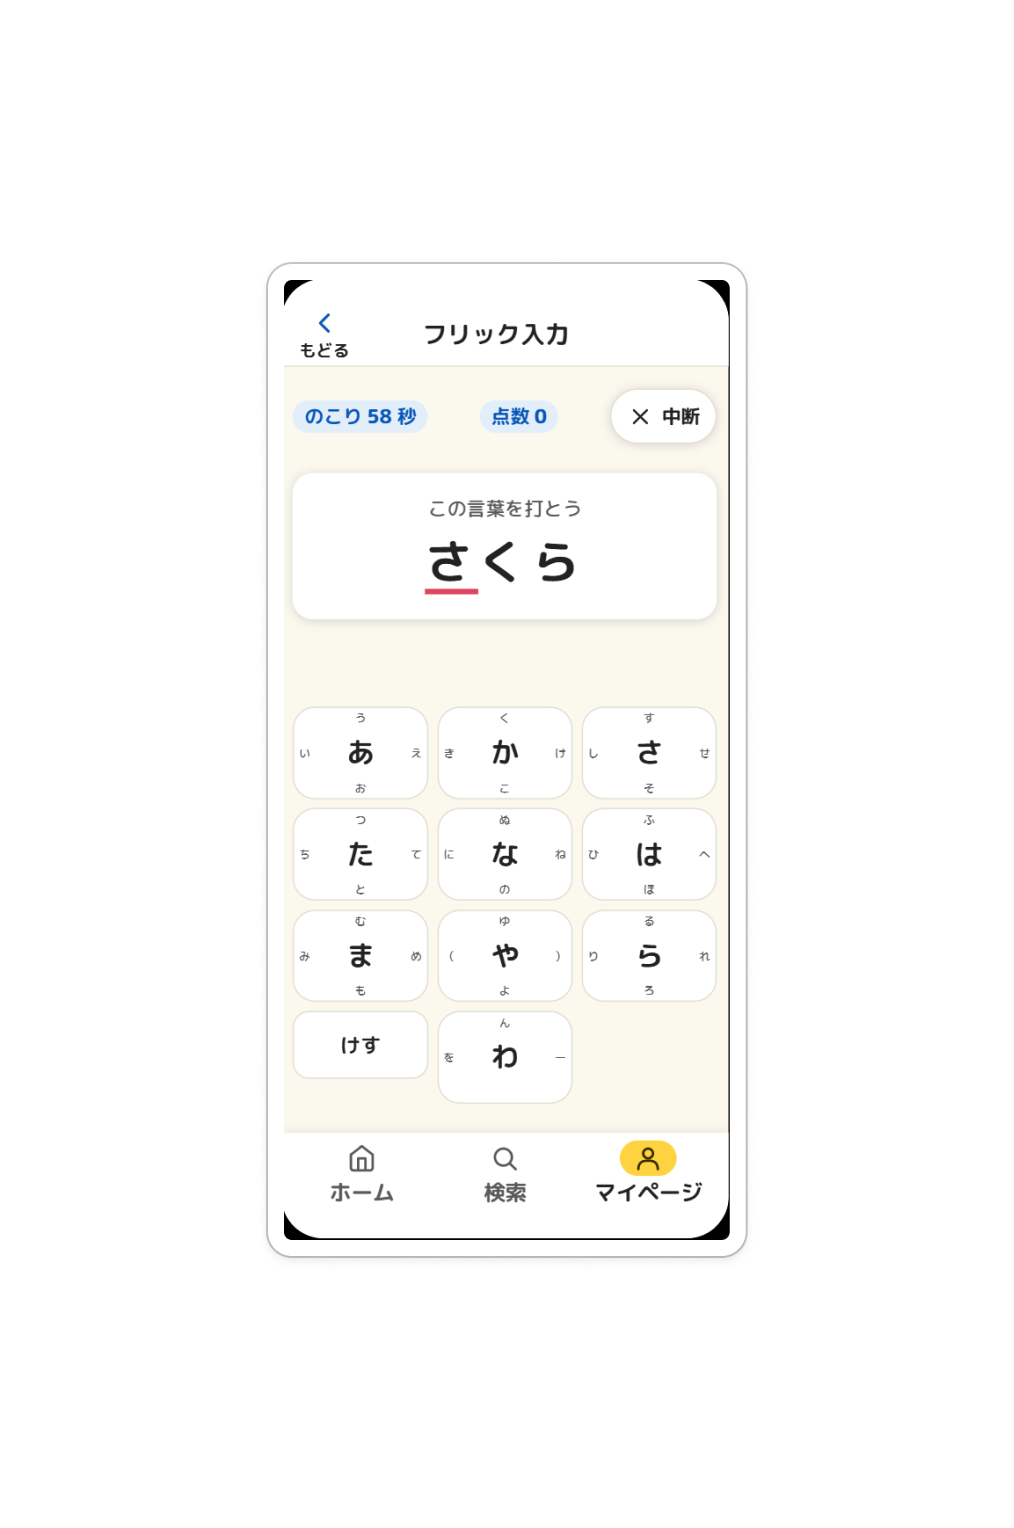
\includegraphics[width=\linewidth]{chapters/images/UI_Screen/lerner/minigame2.png}
    \caption{フリック入力画面}
    \label{fig:minigame2}
  \end{subfigure}

  \caption{ミニゲーム画面}
  \label{fig:minigames}
\end{figure}


\subsubsection{質問画面}

図\ref{fig:question}は、投稿者へ送った質問一覧と、回答がある場合はその回答を見ることができる画面である。

\begin{figure}[H]
  \centering
  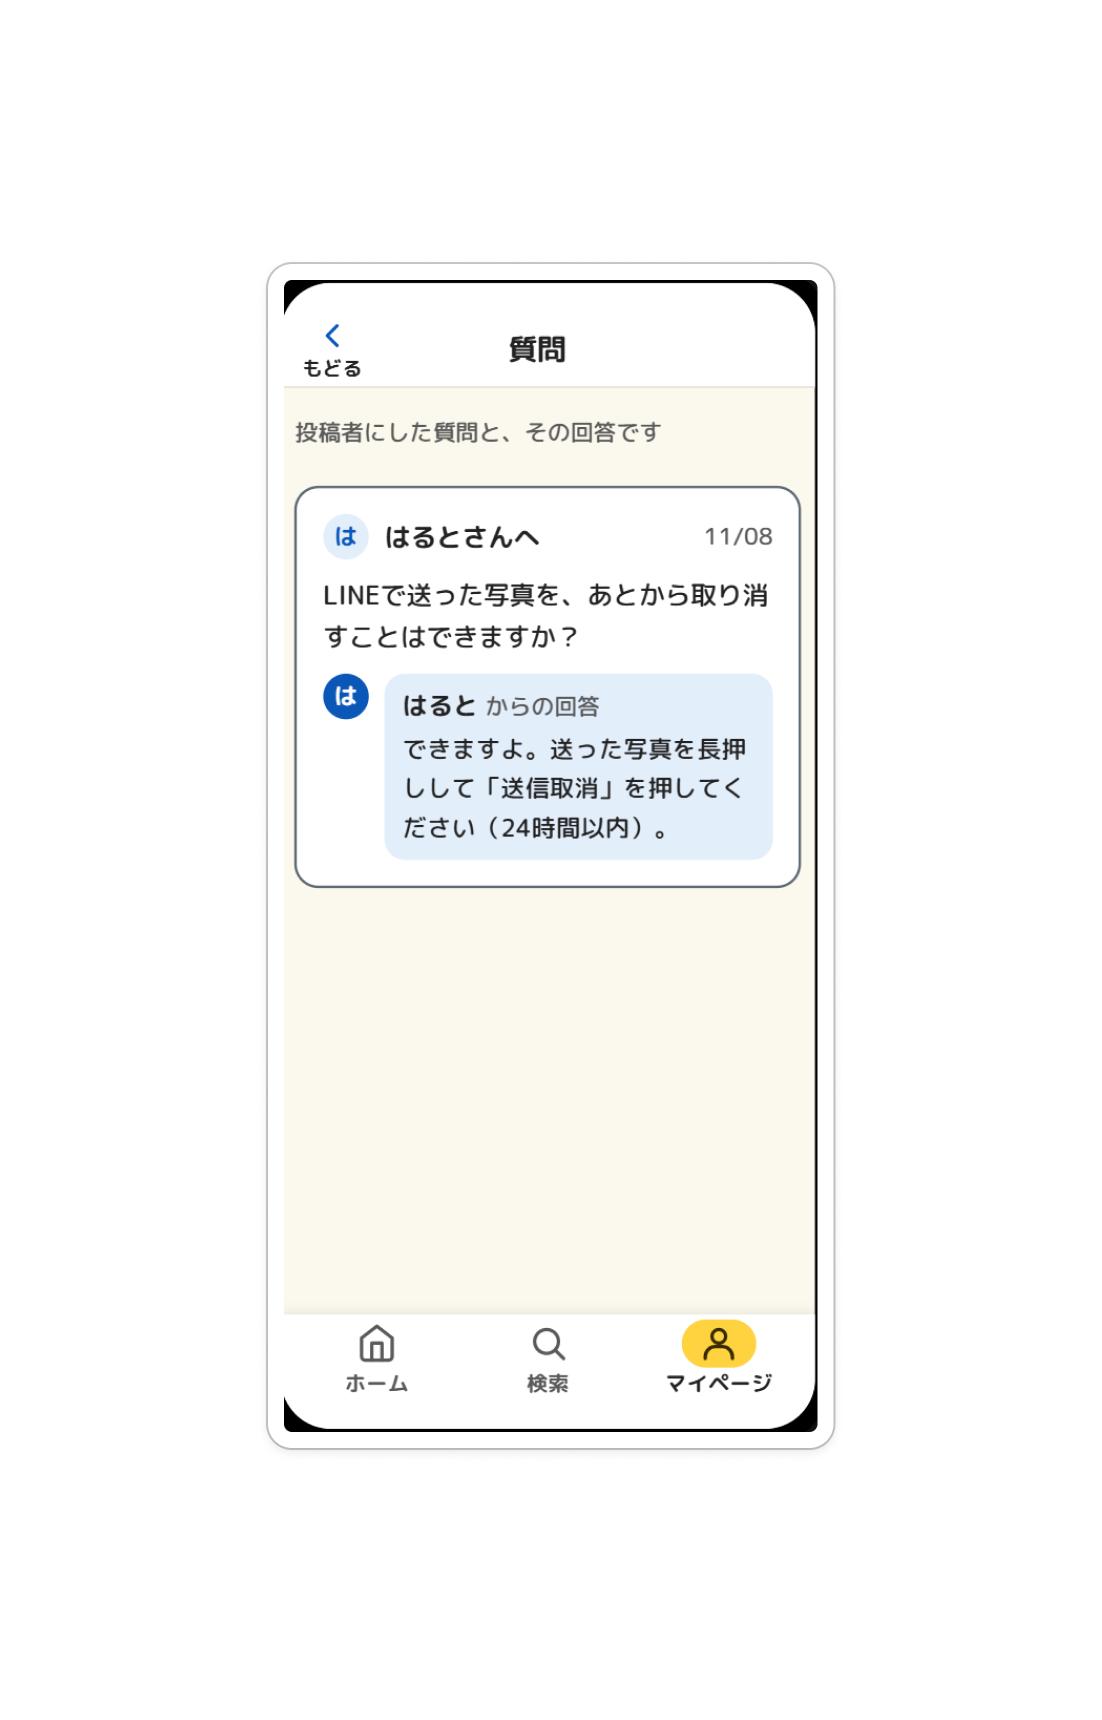
\includegraphics[width=0.55\linewidth]{chapters/images/UI_Screen/lerner/question.png}
  \caption{質問画面}
  \label{fig:question}
\end{figure}


\subsubsection{保存画面}

図\ref{fig:save}は、お気に入りの投稿者、保存した投稿、いいねした投稿の一覧を見ることができる画面である。自動でカテゴリ別に分類される。

\begin{figure}[H]
  \centering
  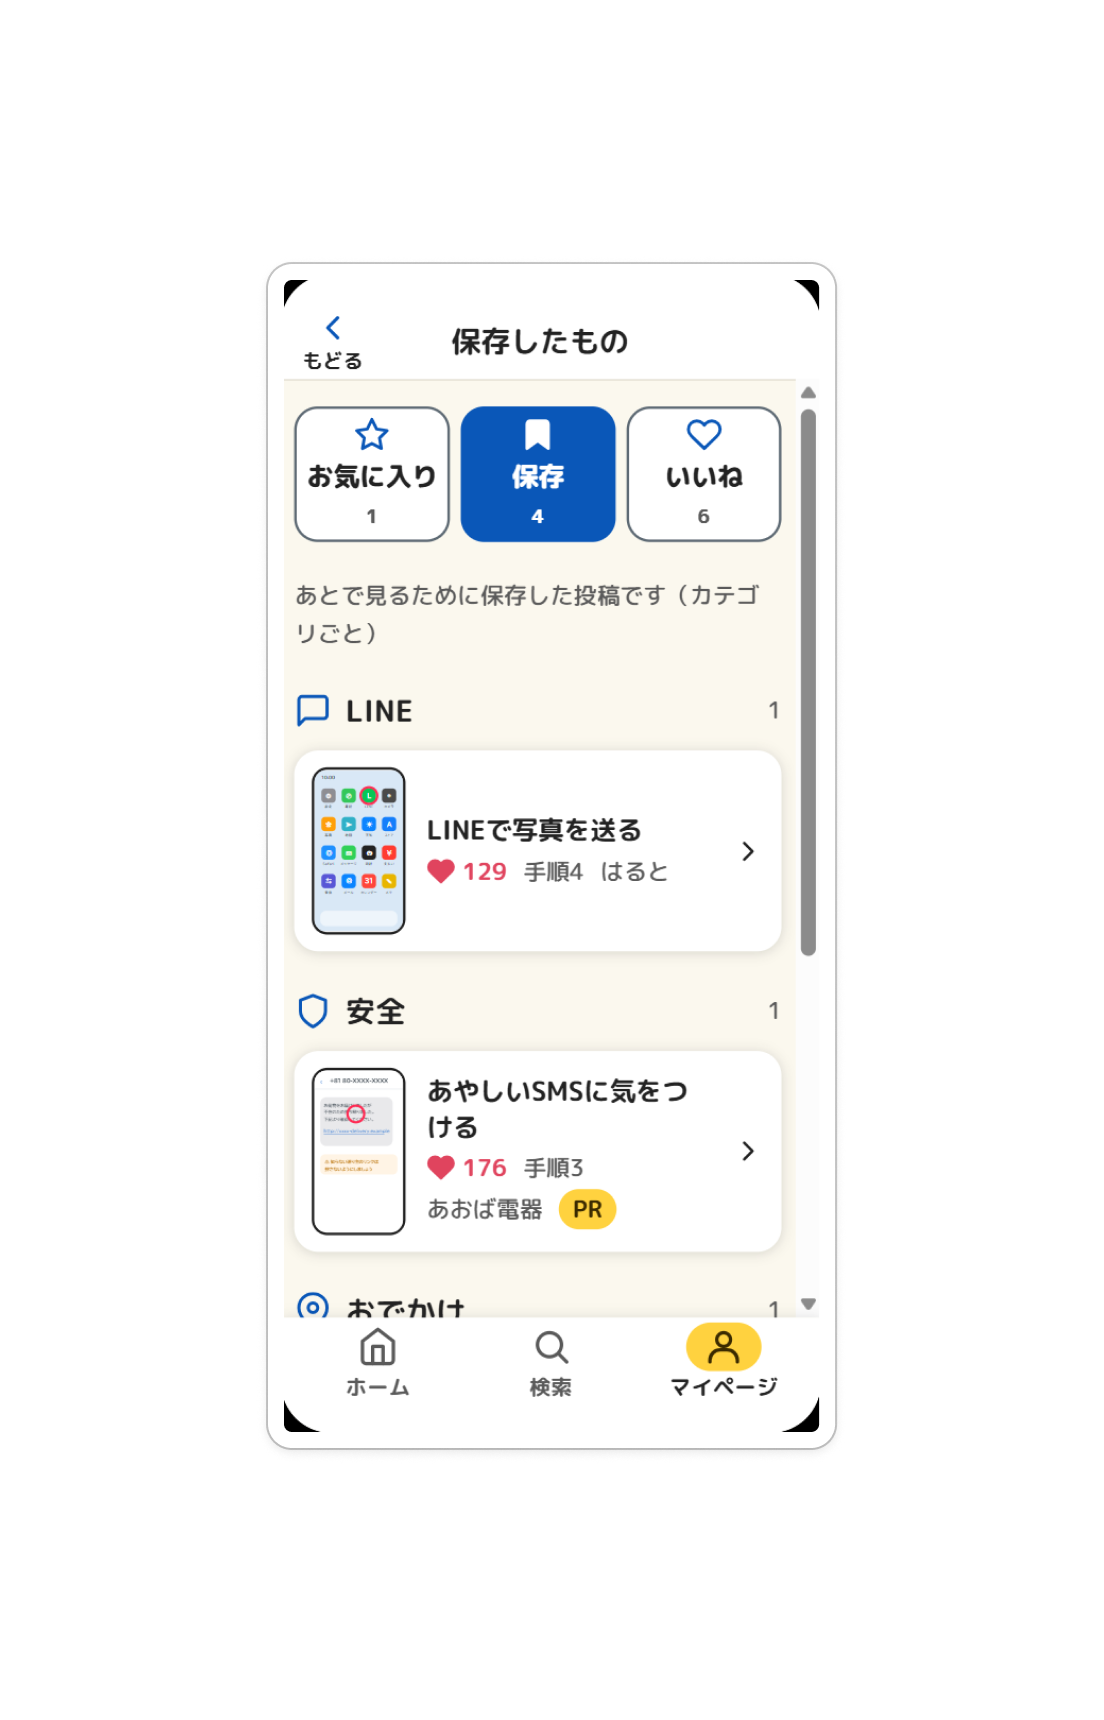
\includegraphics[width=0.55\linewidth]{chapters/images/UI_Screen/lerner/save.png}
  \caption{保存画面}
  \label{fig:save}
\end{figure}


% =================================
\subsection{投稿者画面}
% =================================

\subsubsection{ホーム画面}

図\ref{fig:ad_home}は、管理者のホーム画面である。上部のダッシュボードには、AI要確認・通報・問い合わせの未対応件数と、全投稿数・利用者数・今月の投稿数・月間アクティブ数が表示される。未対応件数をクリックすると、該当する一覧画面へ遷移する。中央には「ユーザ管理」「投稿管理」「詳細管理」の3つのパネルが配置され、未対応がある場合は件数が表示される。右上には現在の権限が表示される。

\begin{figure}[H]
  \centering
  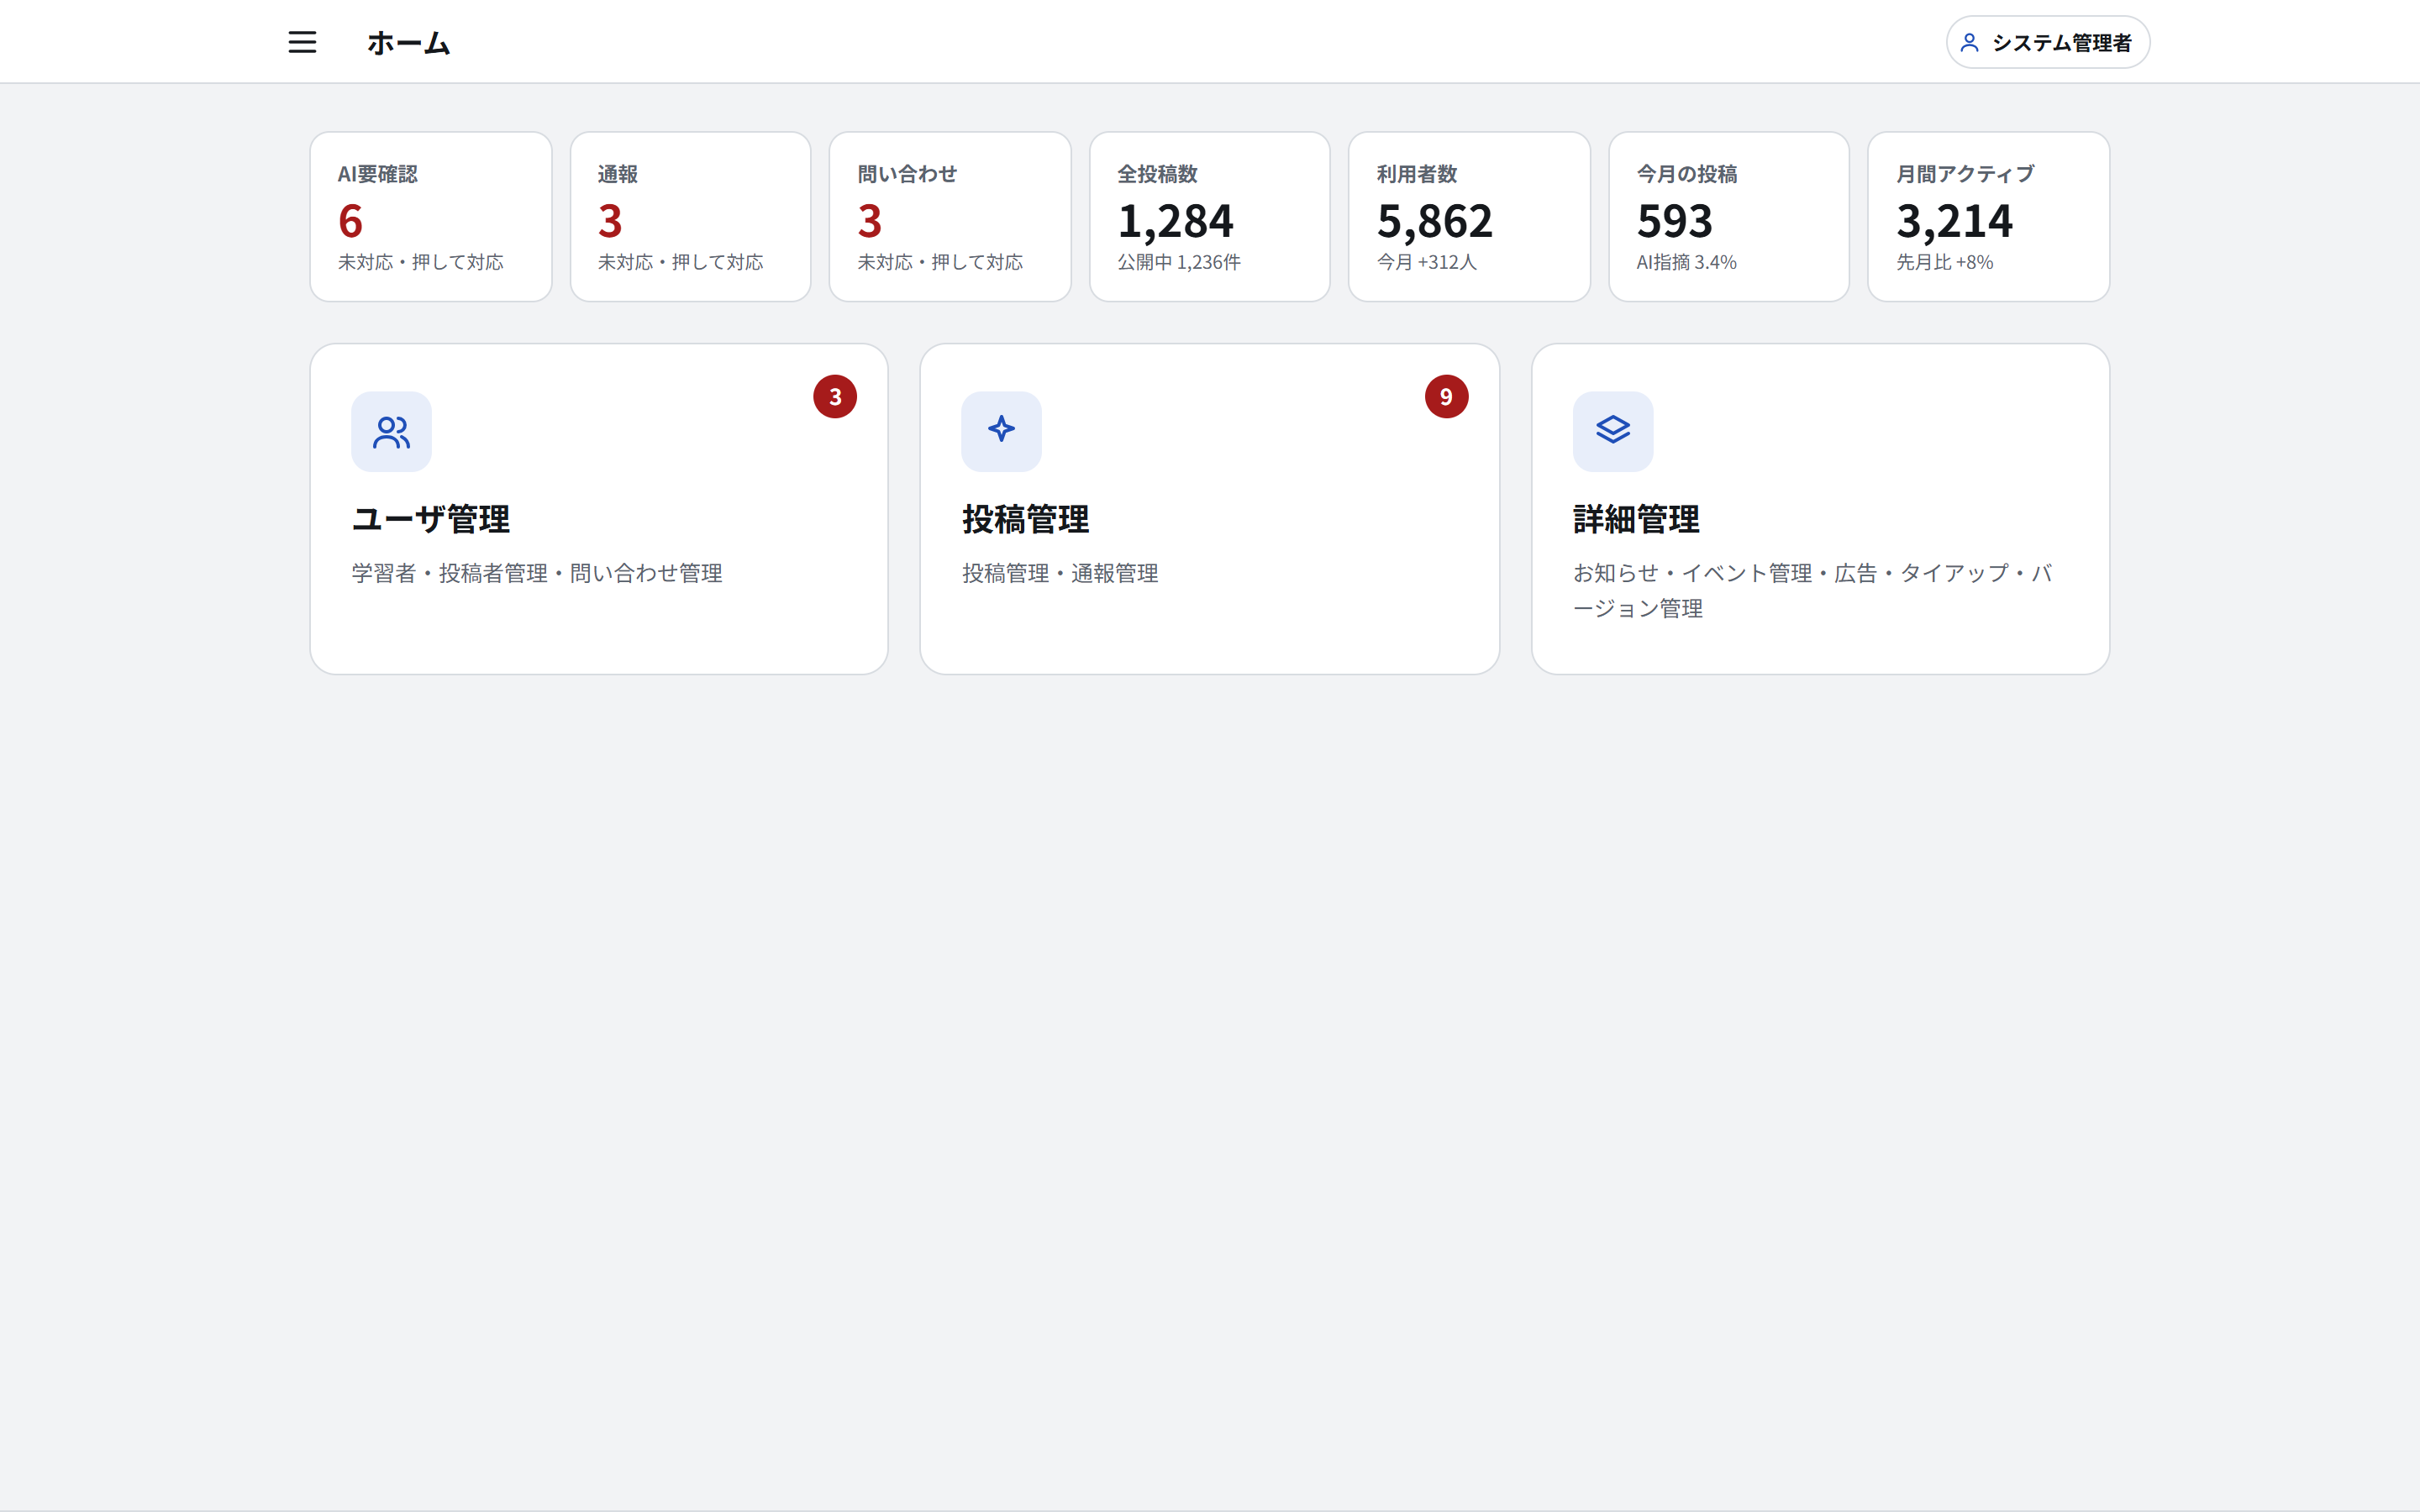
\includegraphics[width=\linewidth]{chapters/images/UI_Screen/admin/home.png}
  \caption{管理者ホーム画面}
  \label{fig:ad_home}
\end{figure}


\subsubsection{メニュー}

図\ref{fig:ad_menu}は、左上のメニューボタンをクリックすると表示されるメニューである。「権限」と「設定」の各画面へ遷移することができる。

\begin{figure}[H]
  \centering
  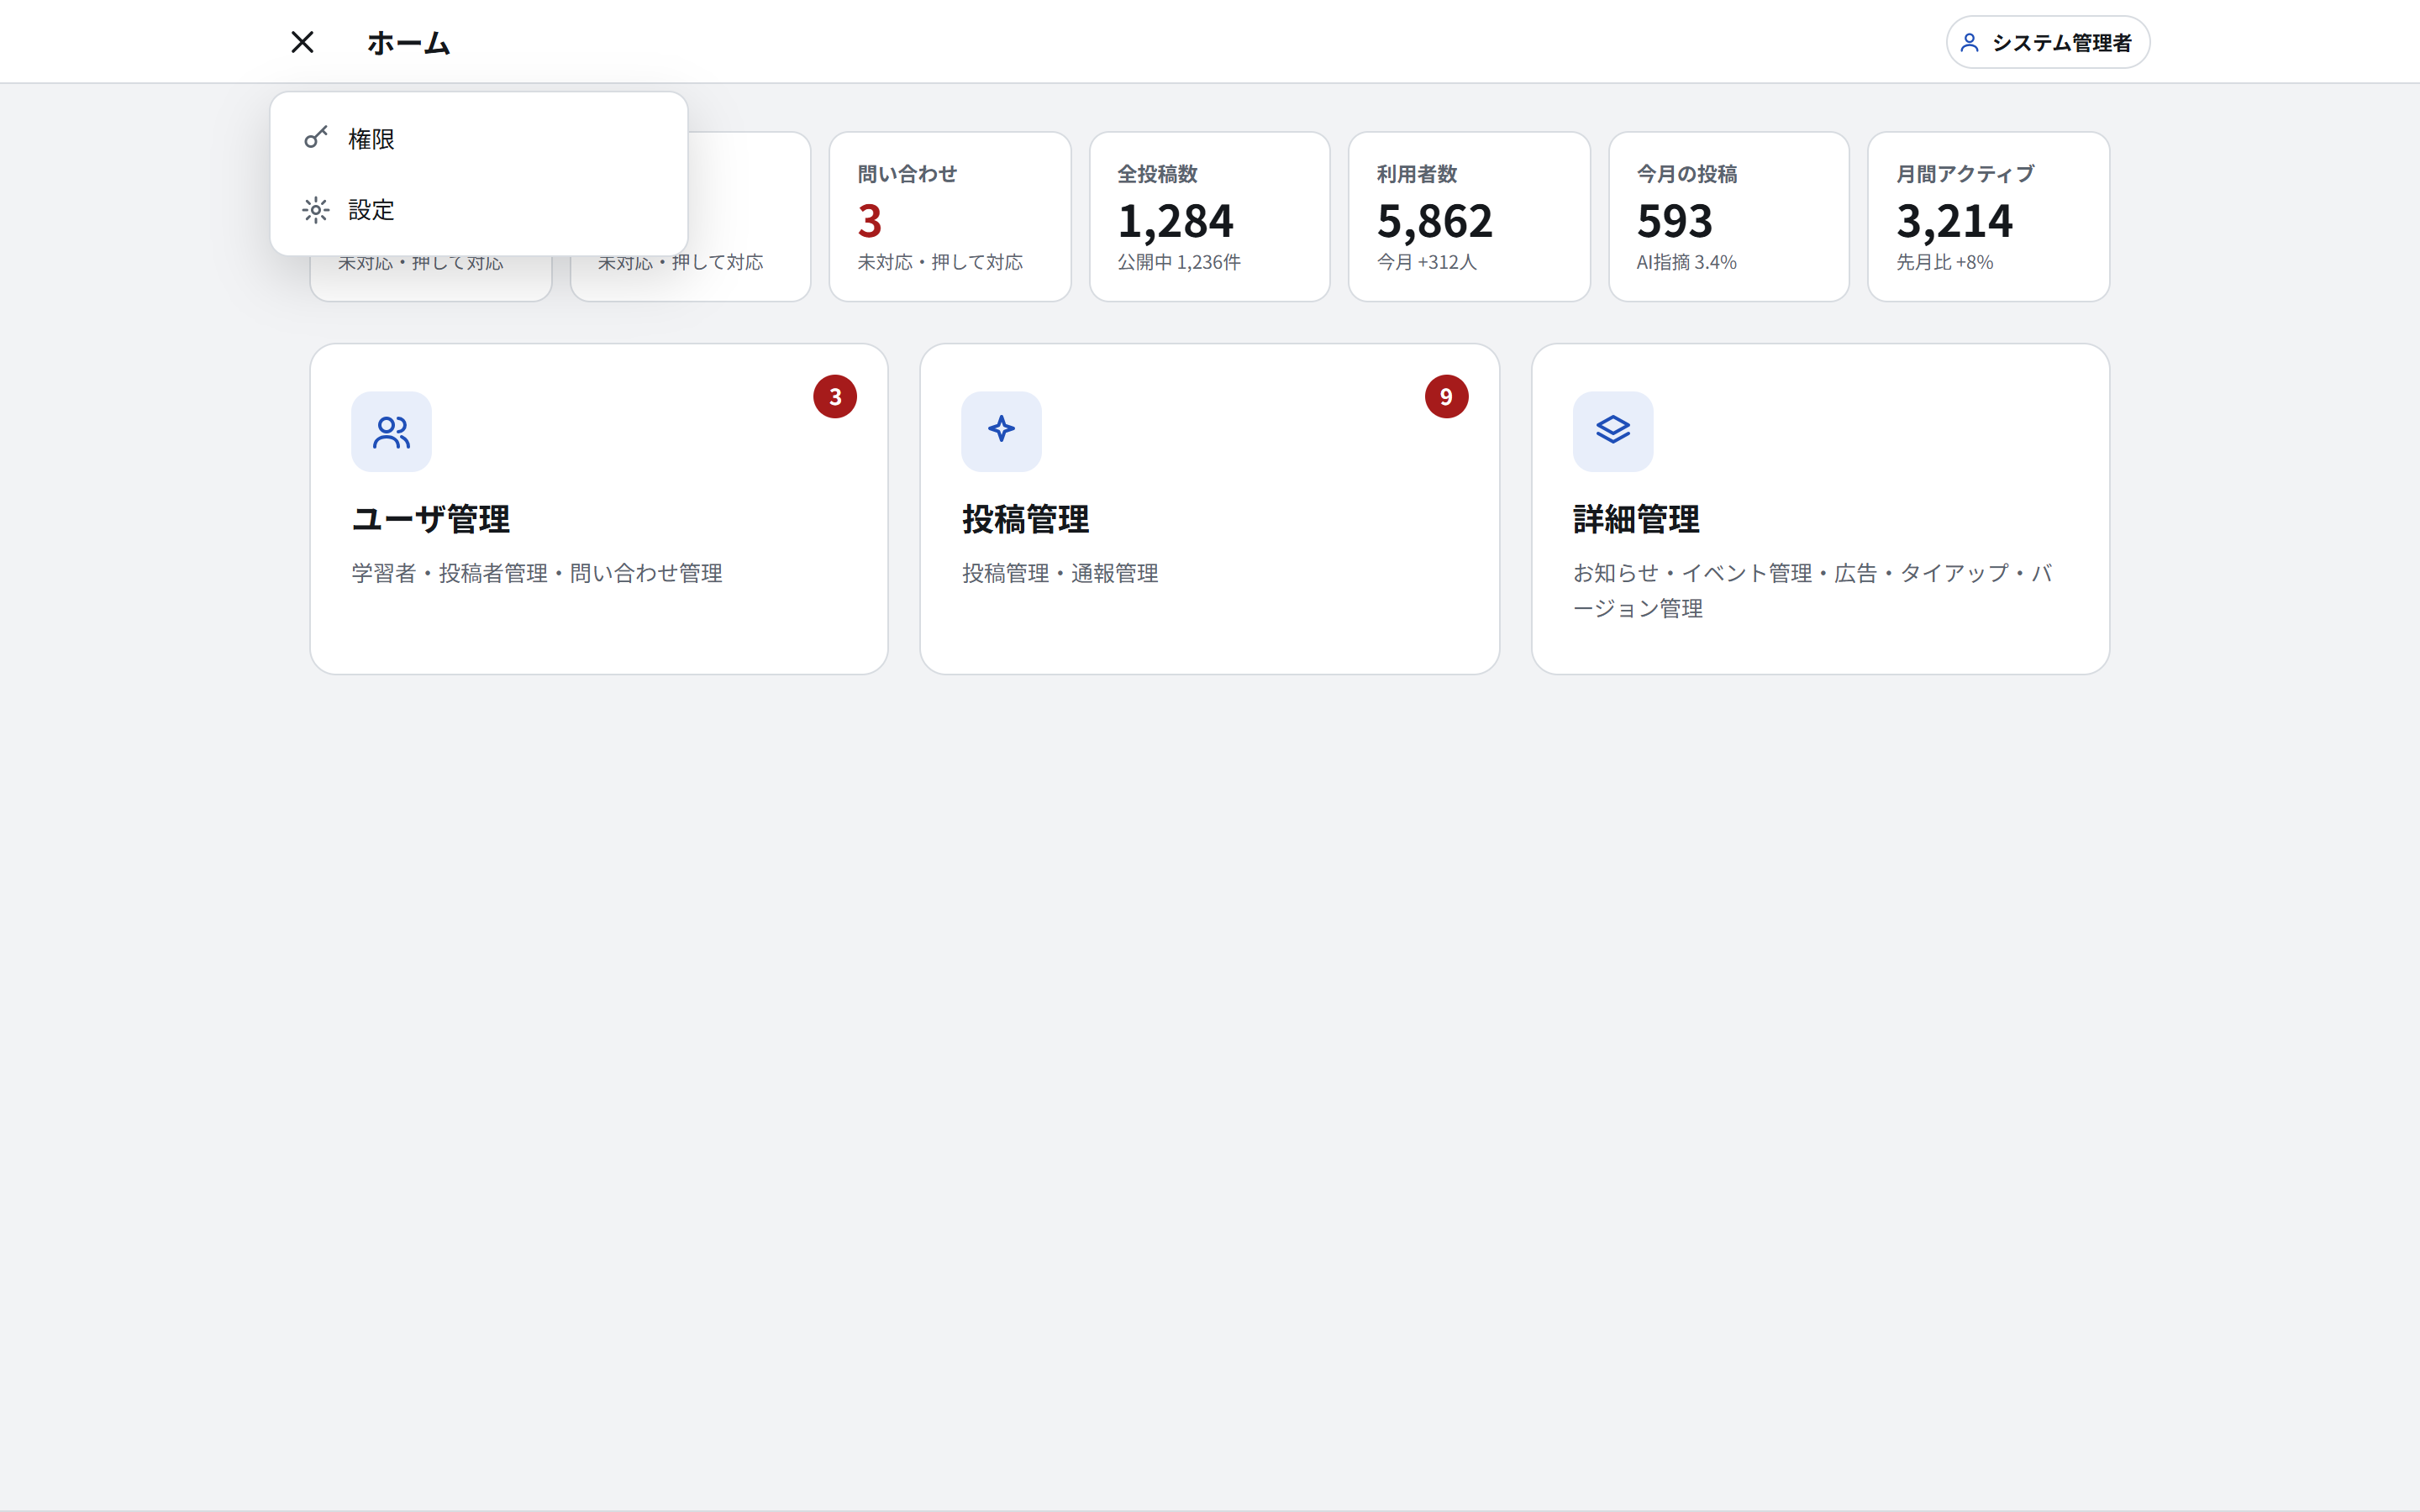
\includegraphics[width=\linewidth]{chapters/images/UI_Screen/admin/menu.png}
  \caption{メニュー}
  \label{fig:ad_menu}
\end{figure}


% =================================
\subsection{ユーザ管理画面}
% =================================

\subsubsection{ユーザ管理（パネル一覧）画面}

図\ref{fig:ad_user_panel}は、ホーム画面で「ユーザ管理」をクリックすると表示される画面である。「学習者・投稿者管理」と「問い合わせ管理」のパネルが配置され、クリックするとそれぞれの画面へ遷移する。

\begin{figure}[H]
  \centering
  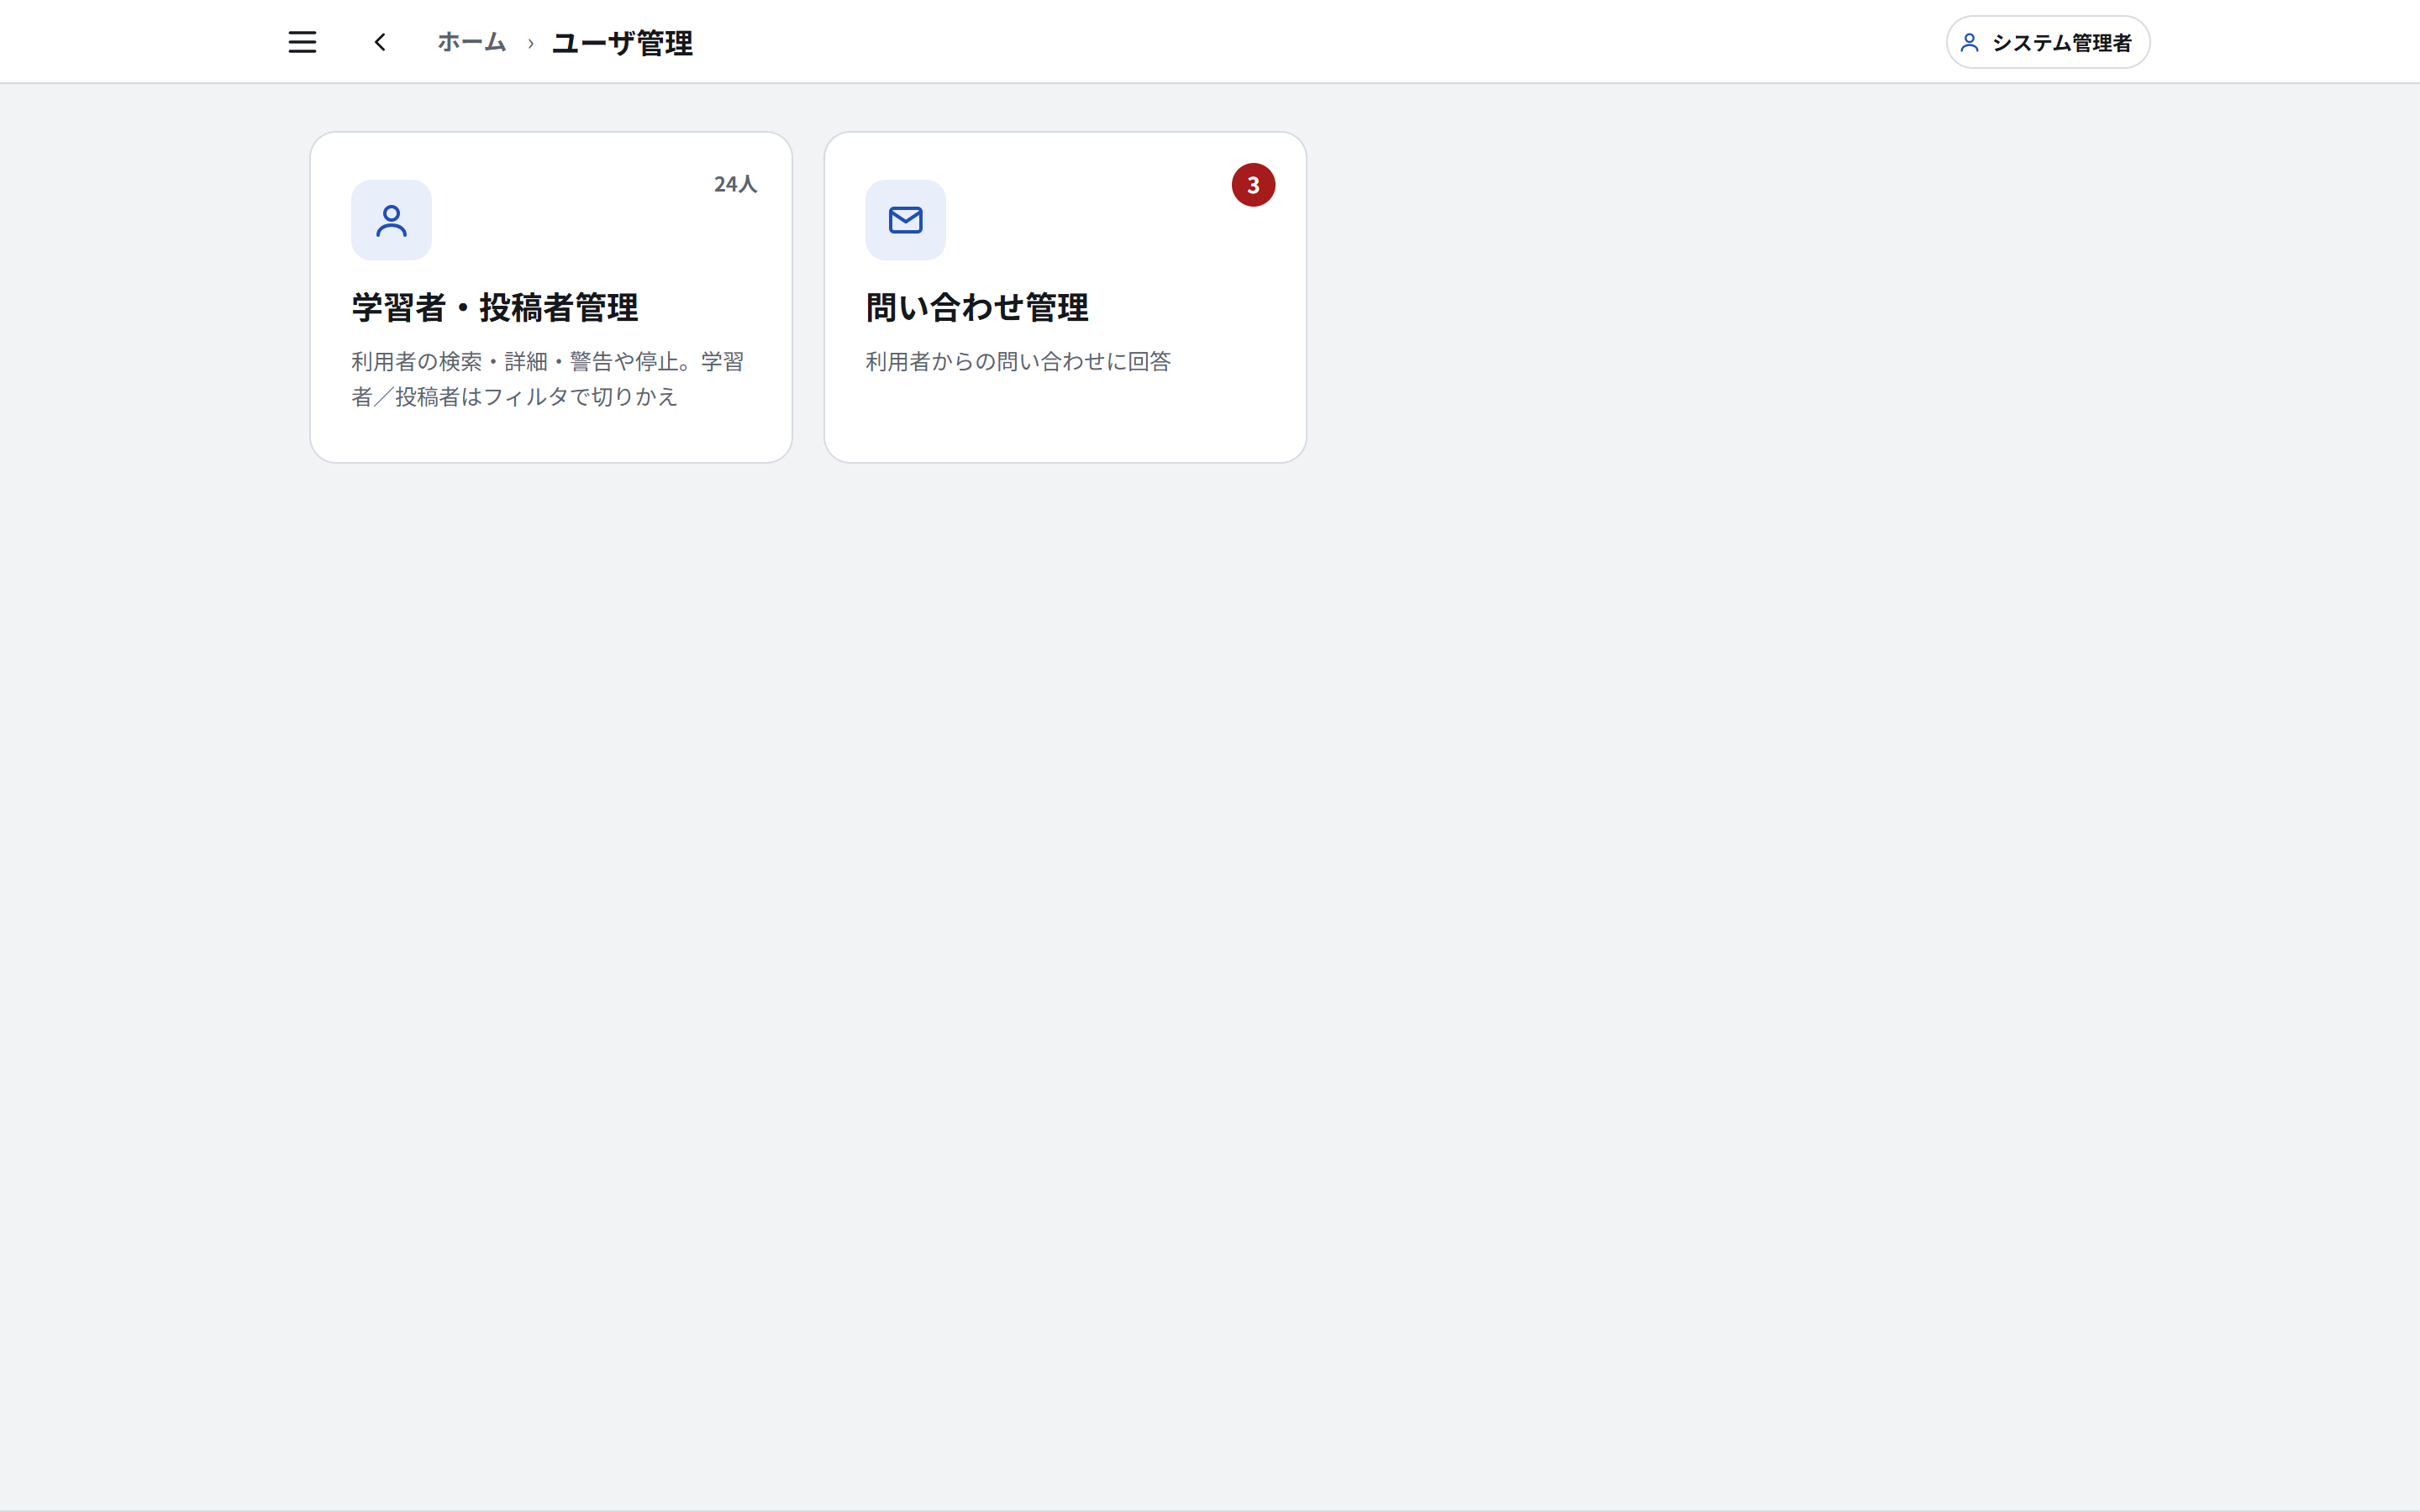
\includegraphics[width=\linewidth]{chapters/images/UI_Screen/admin/user_panel.png}
  \caption{ユーザ管理（パネル一覧）画面}
  \label{fig:ad_user_panel}
\end{figure}


\subsubsection{学習者・投稿者管理画面}

図\ref{fig:ad_user}は、学習者と投稿者をまとめて一覧表示する画面である。ニックネーム・ID・電話番号で検索することができ、「すべて」「学習者」「投稿者」のフィルタで種別ごとに絞り込むことができる。一覧には種別・電話番号・投稿数・通報数・利用状態が表示され、行をクリックすると利用者詳細画面へ遷移する。

\begin{figure}[H]
  \centering
  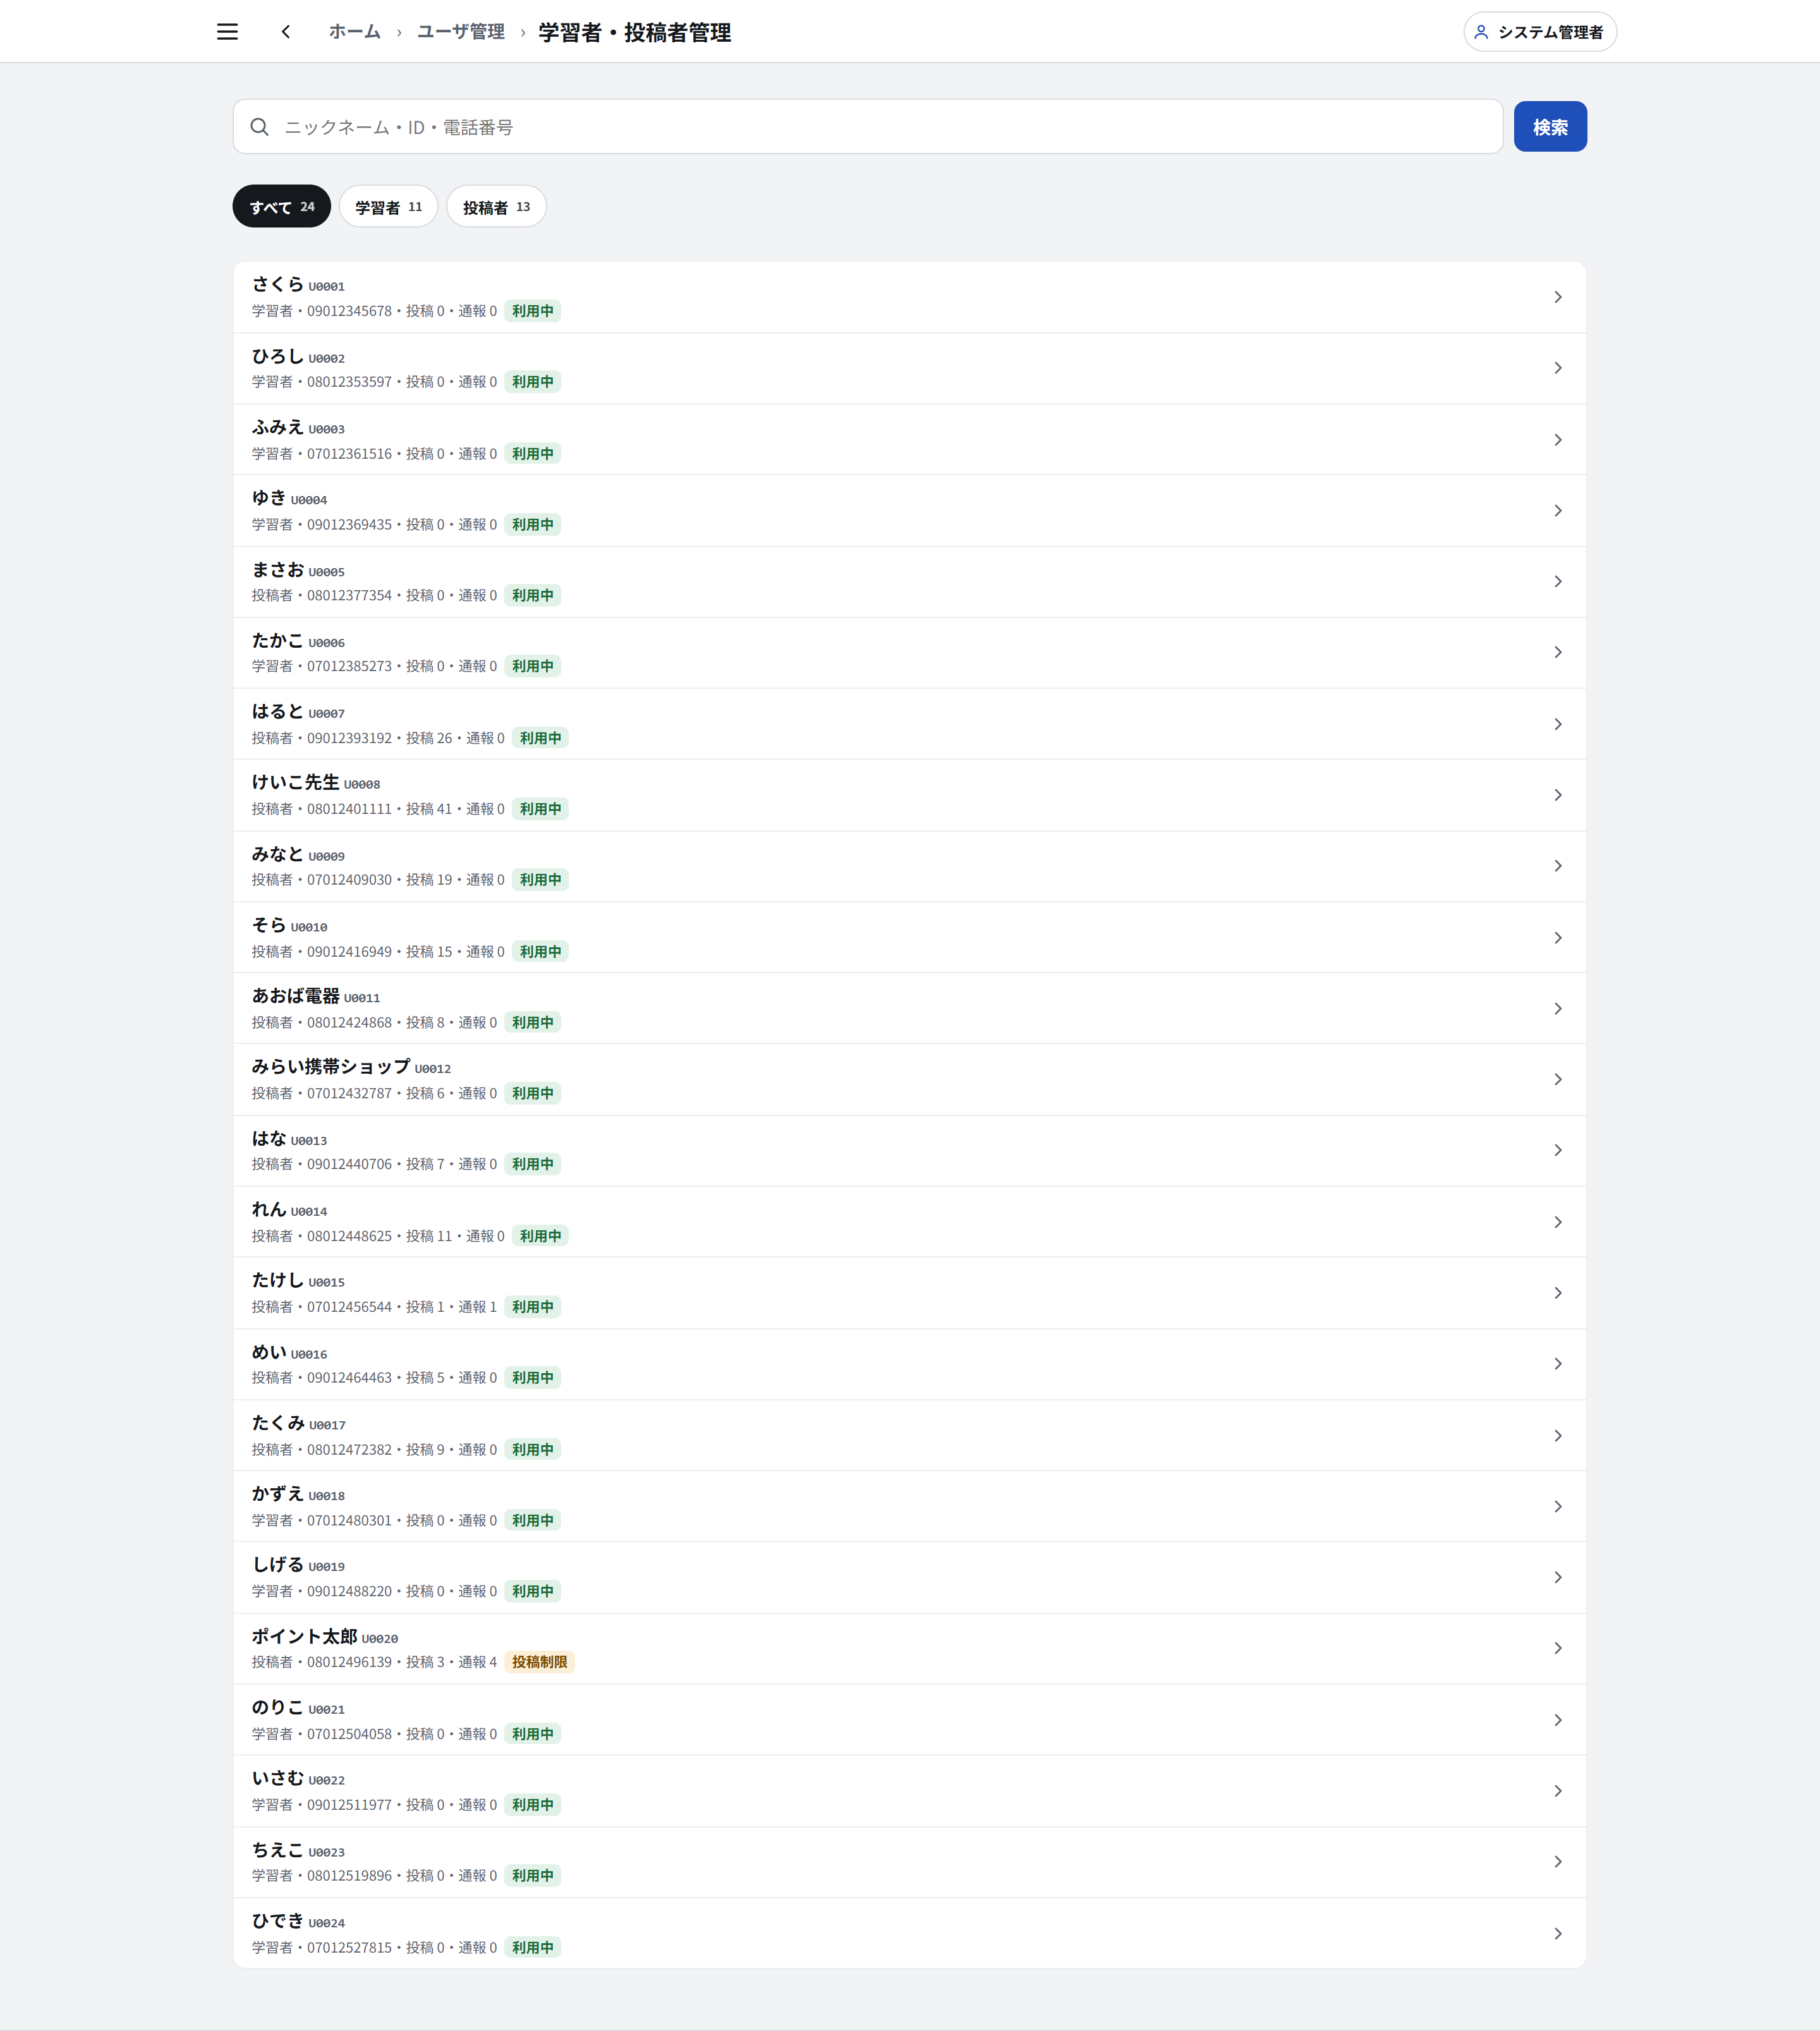
\includegraphics[width=0.8\linewidth]{chapters/images/UI_Screen/admin/user.png}
  \caption{学習者・投稿者管理画面}
  \label{fig:ad_user}
\end{figure}

図\ref{fig:ad_user2}は、フィルタで「投稿者」を選択したときの表示である。投稿者のみが一覧に表示される。フィルタには種別ごとの人数が表示される。

\begin{figure}[H]
  \centering
  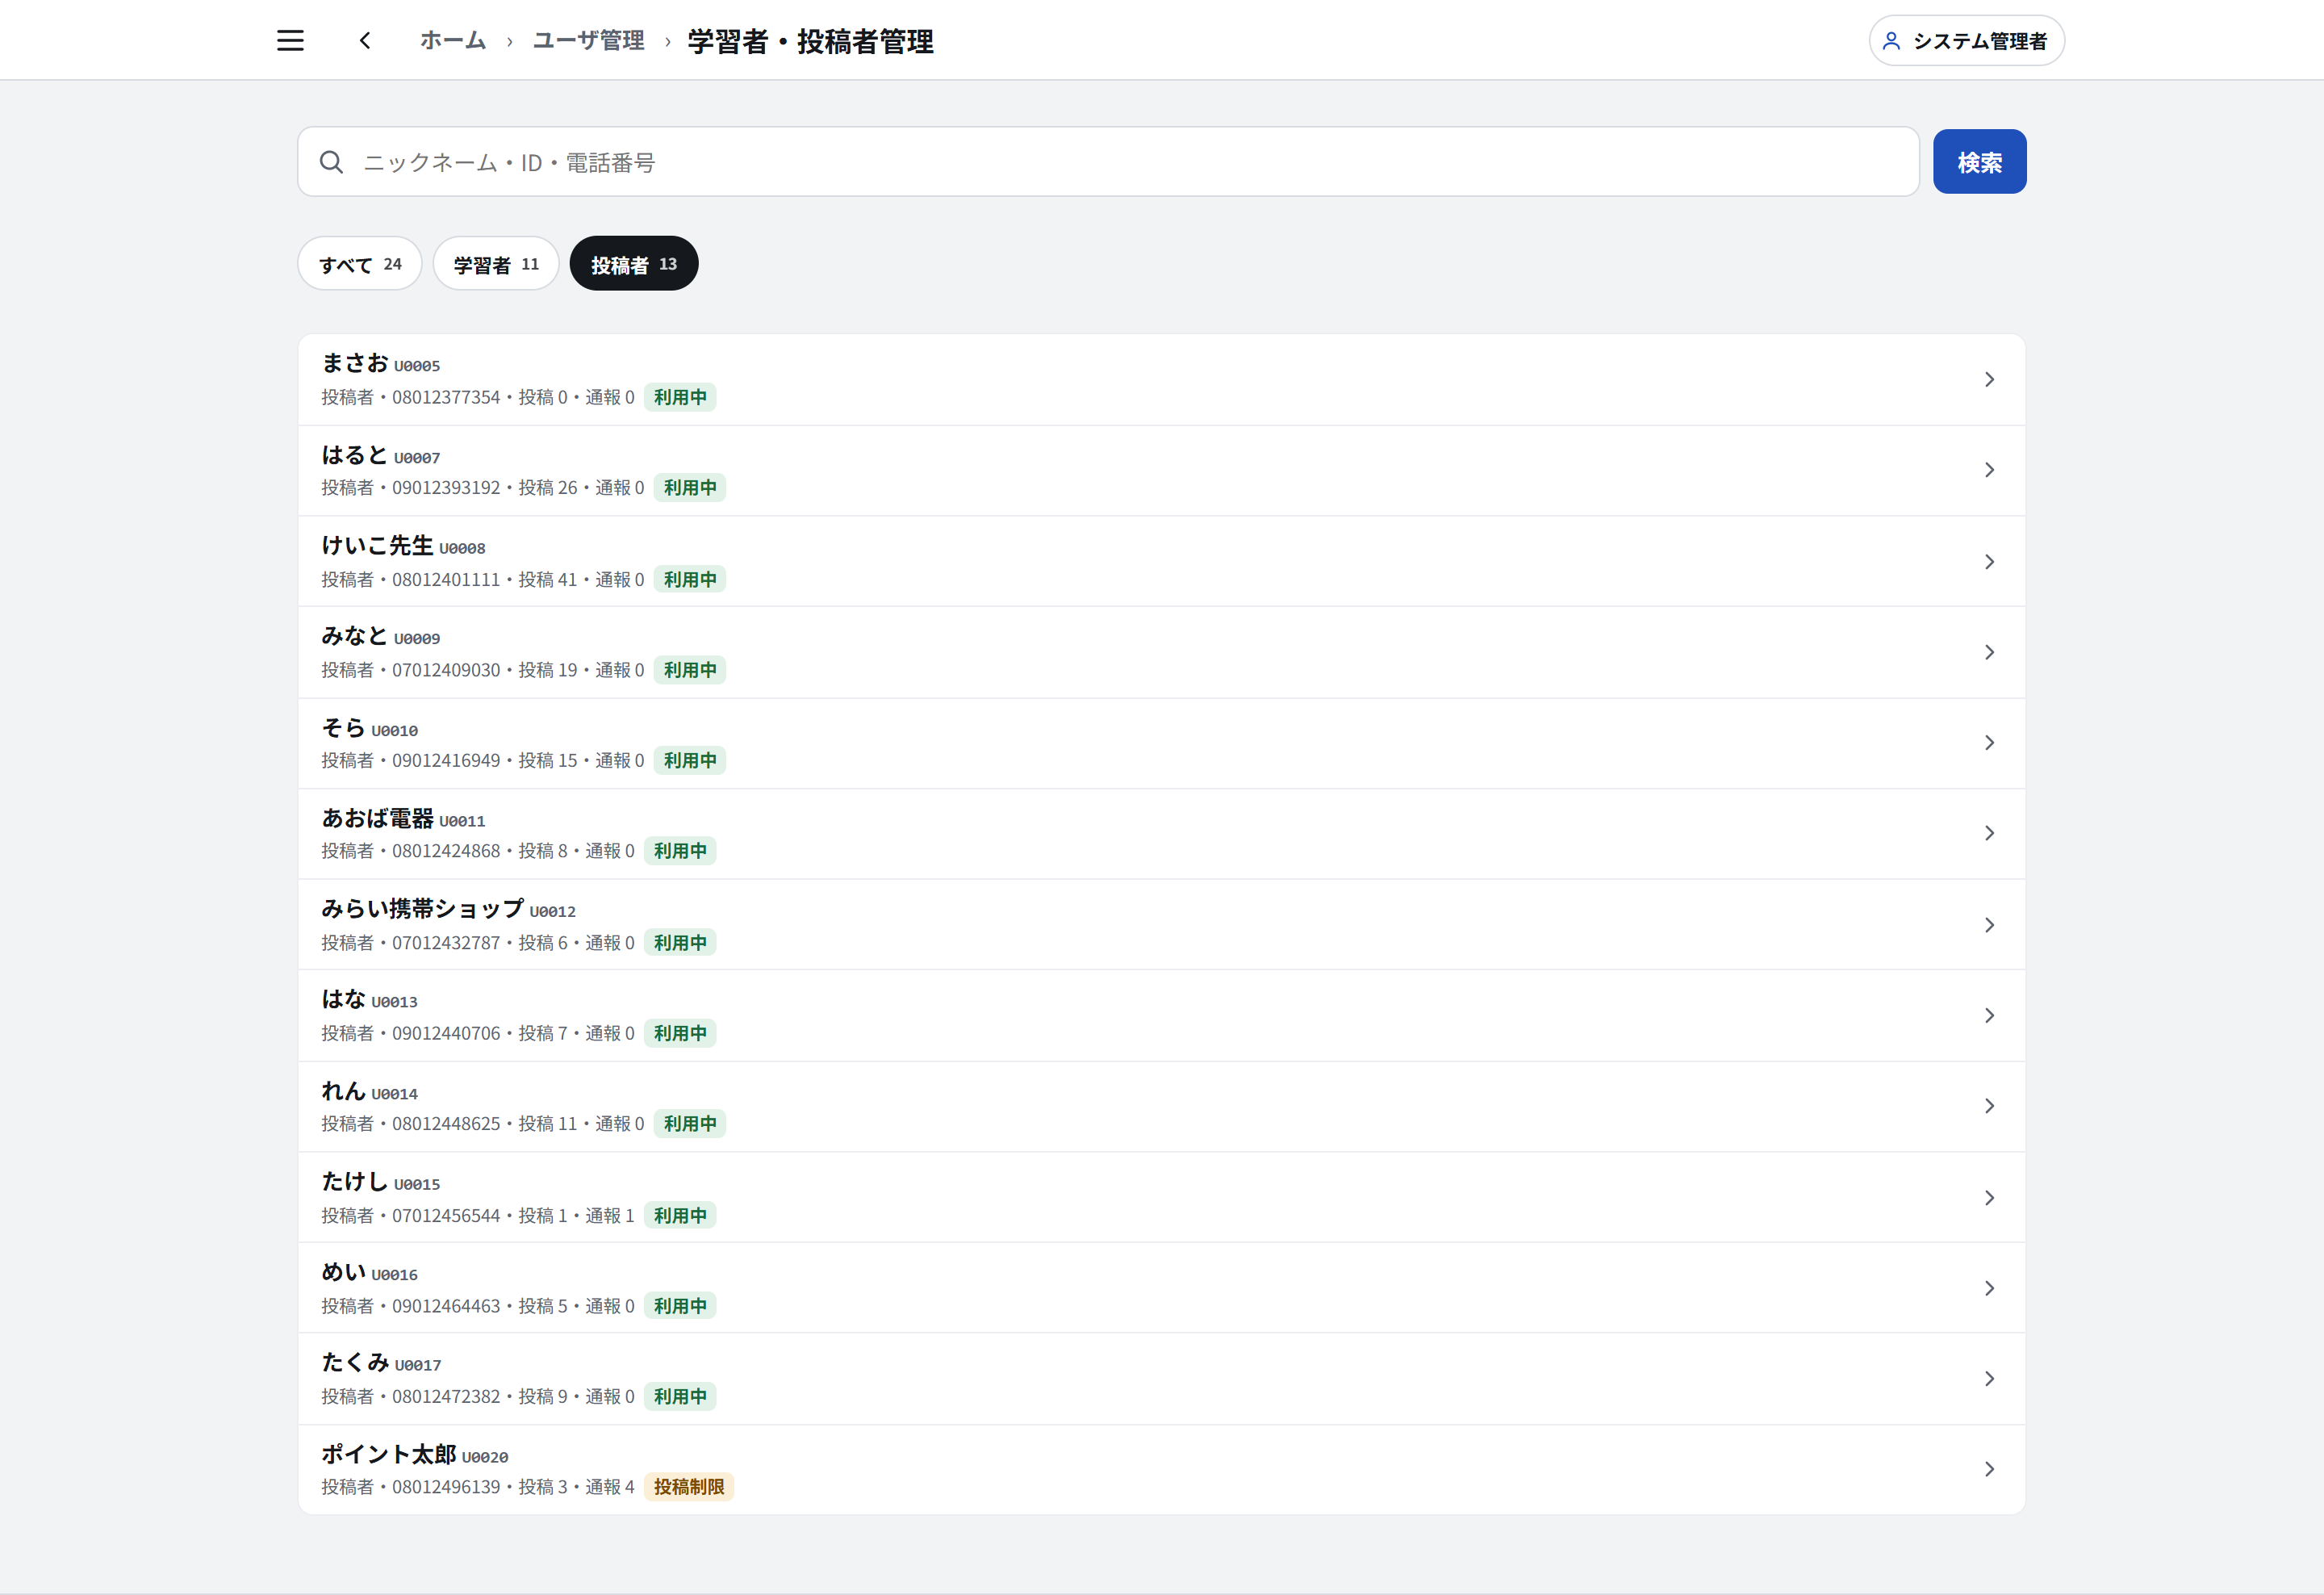
\includegraphics[width=\linewidth]{chapters/images/UI_Screen/admin/user2.png}
  \caption{学習者・投稿者管理画面（投稿者で絞り込み）}
  \label{fig:ad_user2}
\end{figure}

図\ref{fig:ad_user_mask}は、システム管理者以外の権限で開いたときの表示である。本名や電話番号は伏せ字で表示され、電話番号での検索もできない。

\begin{figure}[H]
  \centering
  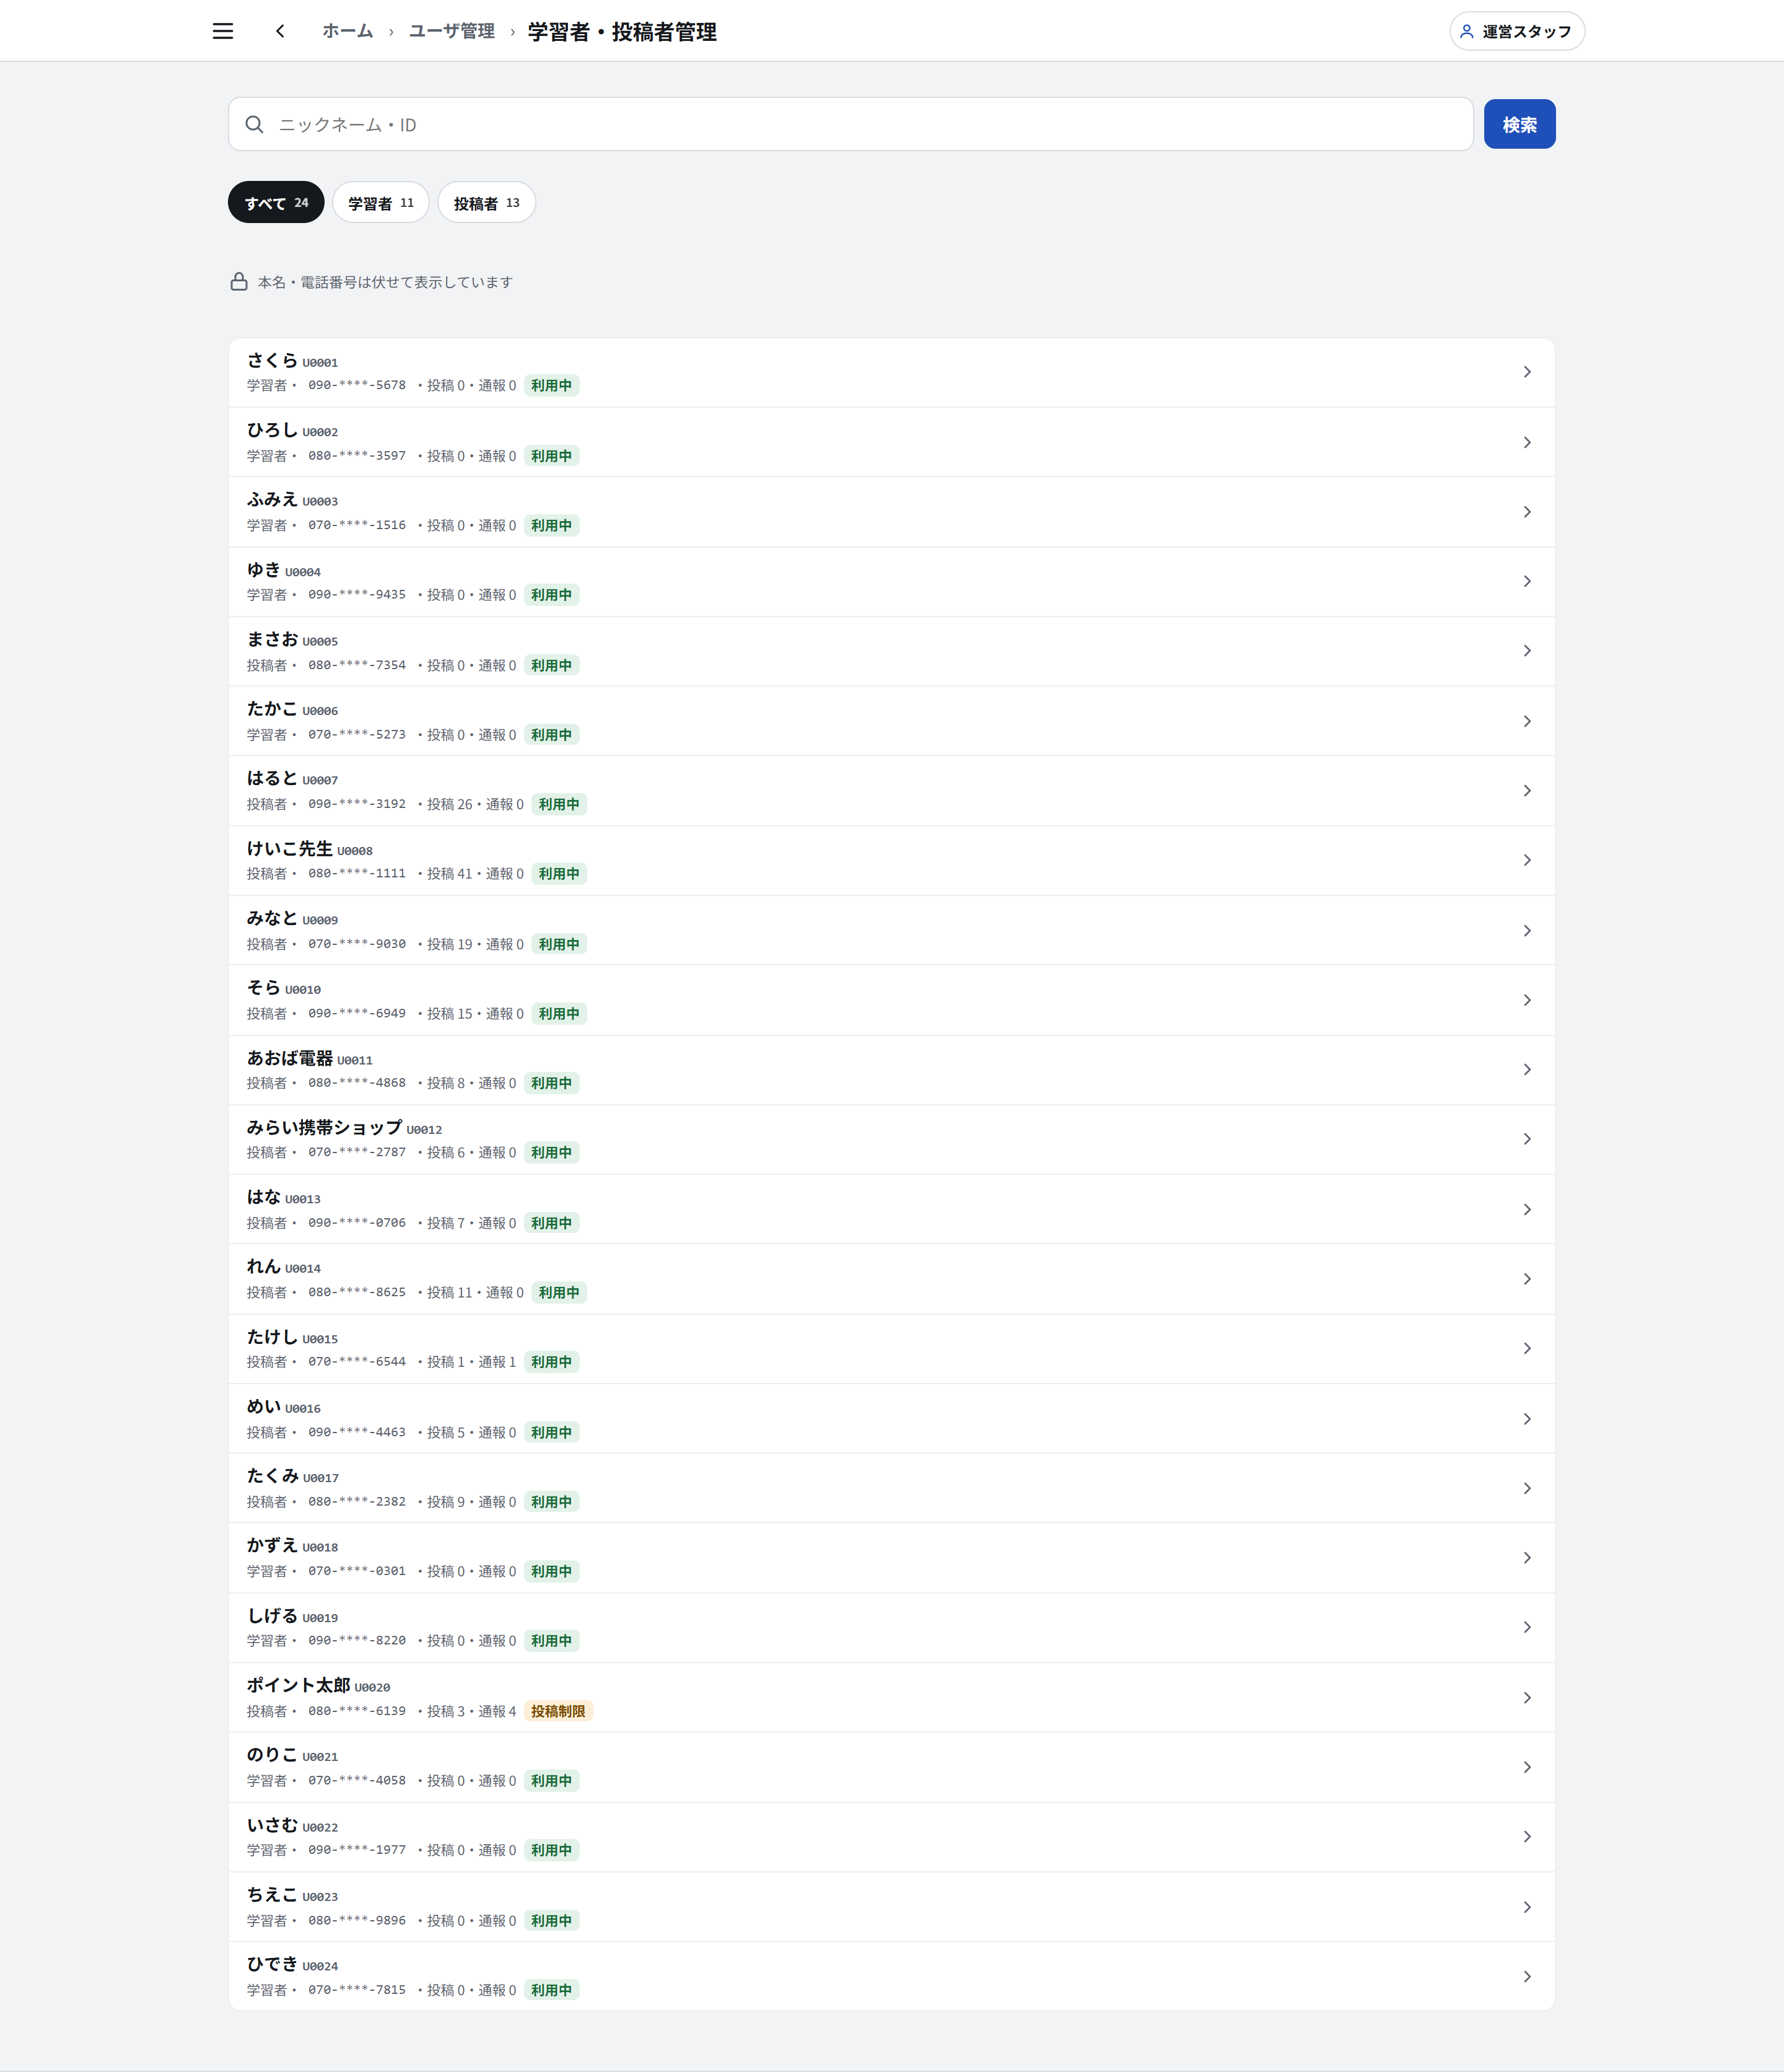
\includegraphics[width=0.8\linewidth]{chapters/images/UI_Screen/admin/user_mask.png}
  \caption{学習者・投稿者管理画面（個人情報を伏せた表示）}
  \label{fig:ad_user_mask}
\end{figure}


\subsubsection{利用者詳細画面}

利用者詳細画面を図\ref{fig:ad_user_details}に示す。

\begin{figure}[H]
  \centering

  \begin{subfigure}[t]{0.48\linewidth}
    \centering
    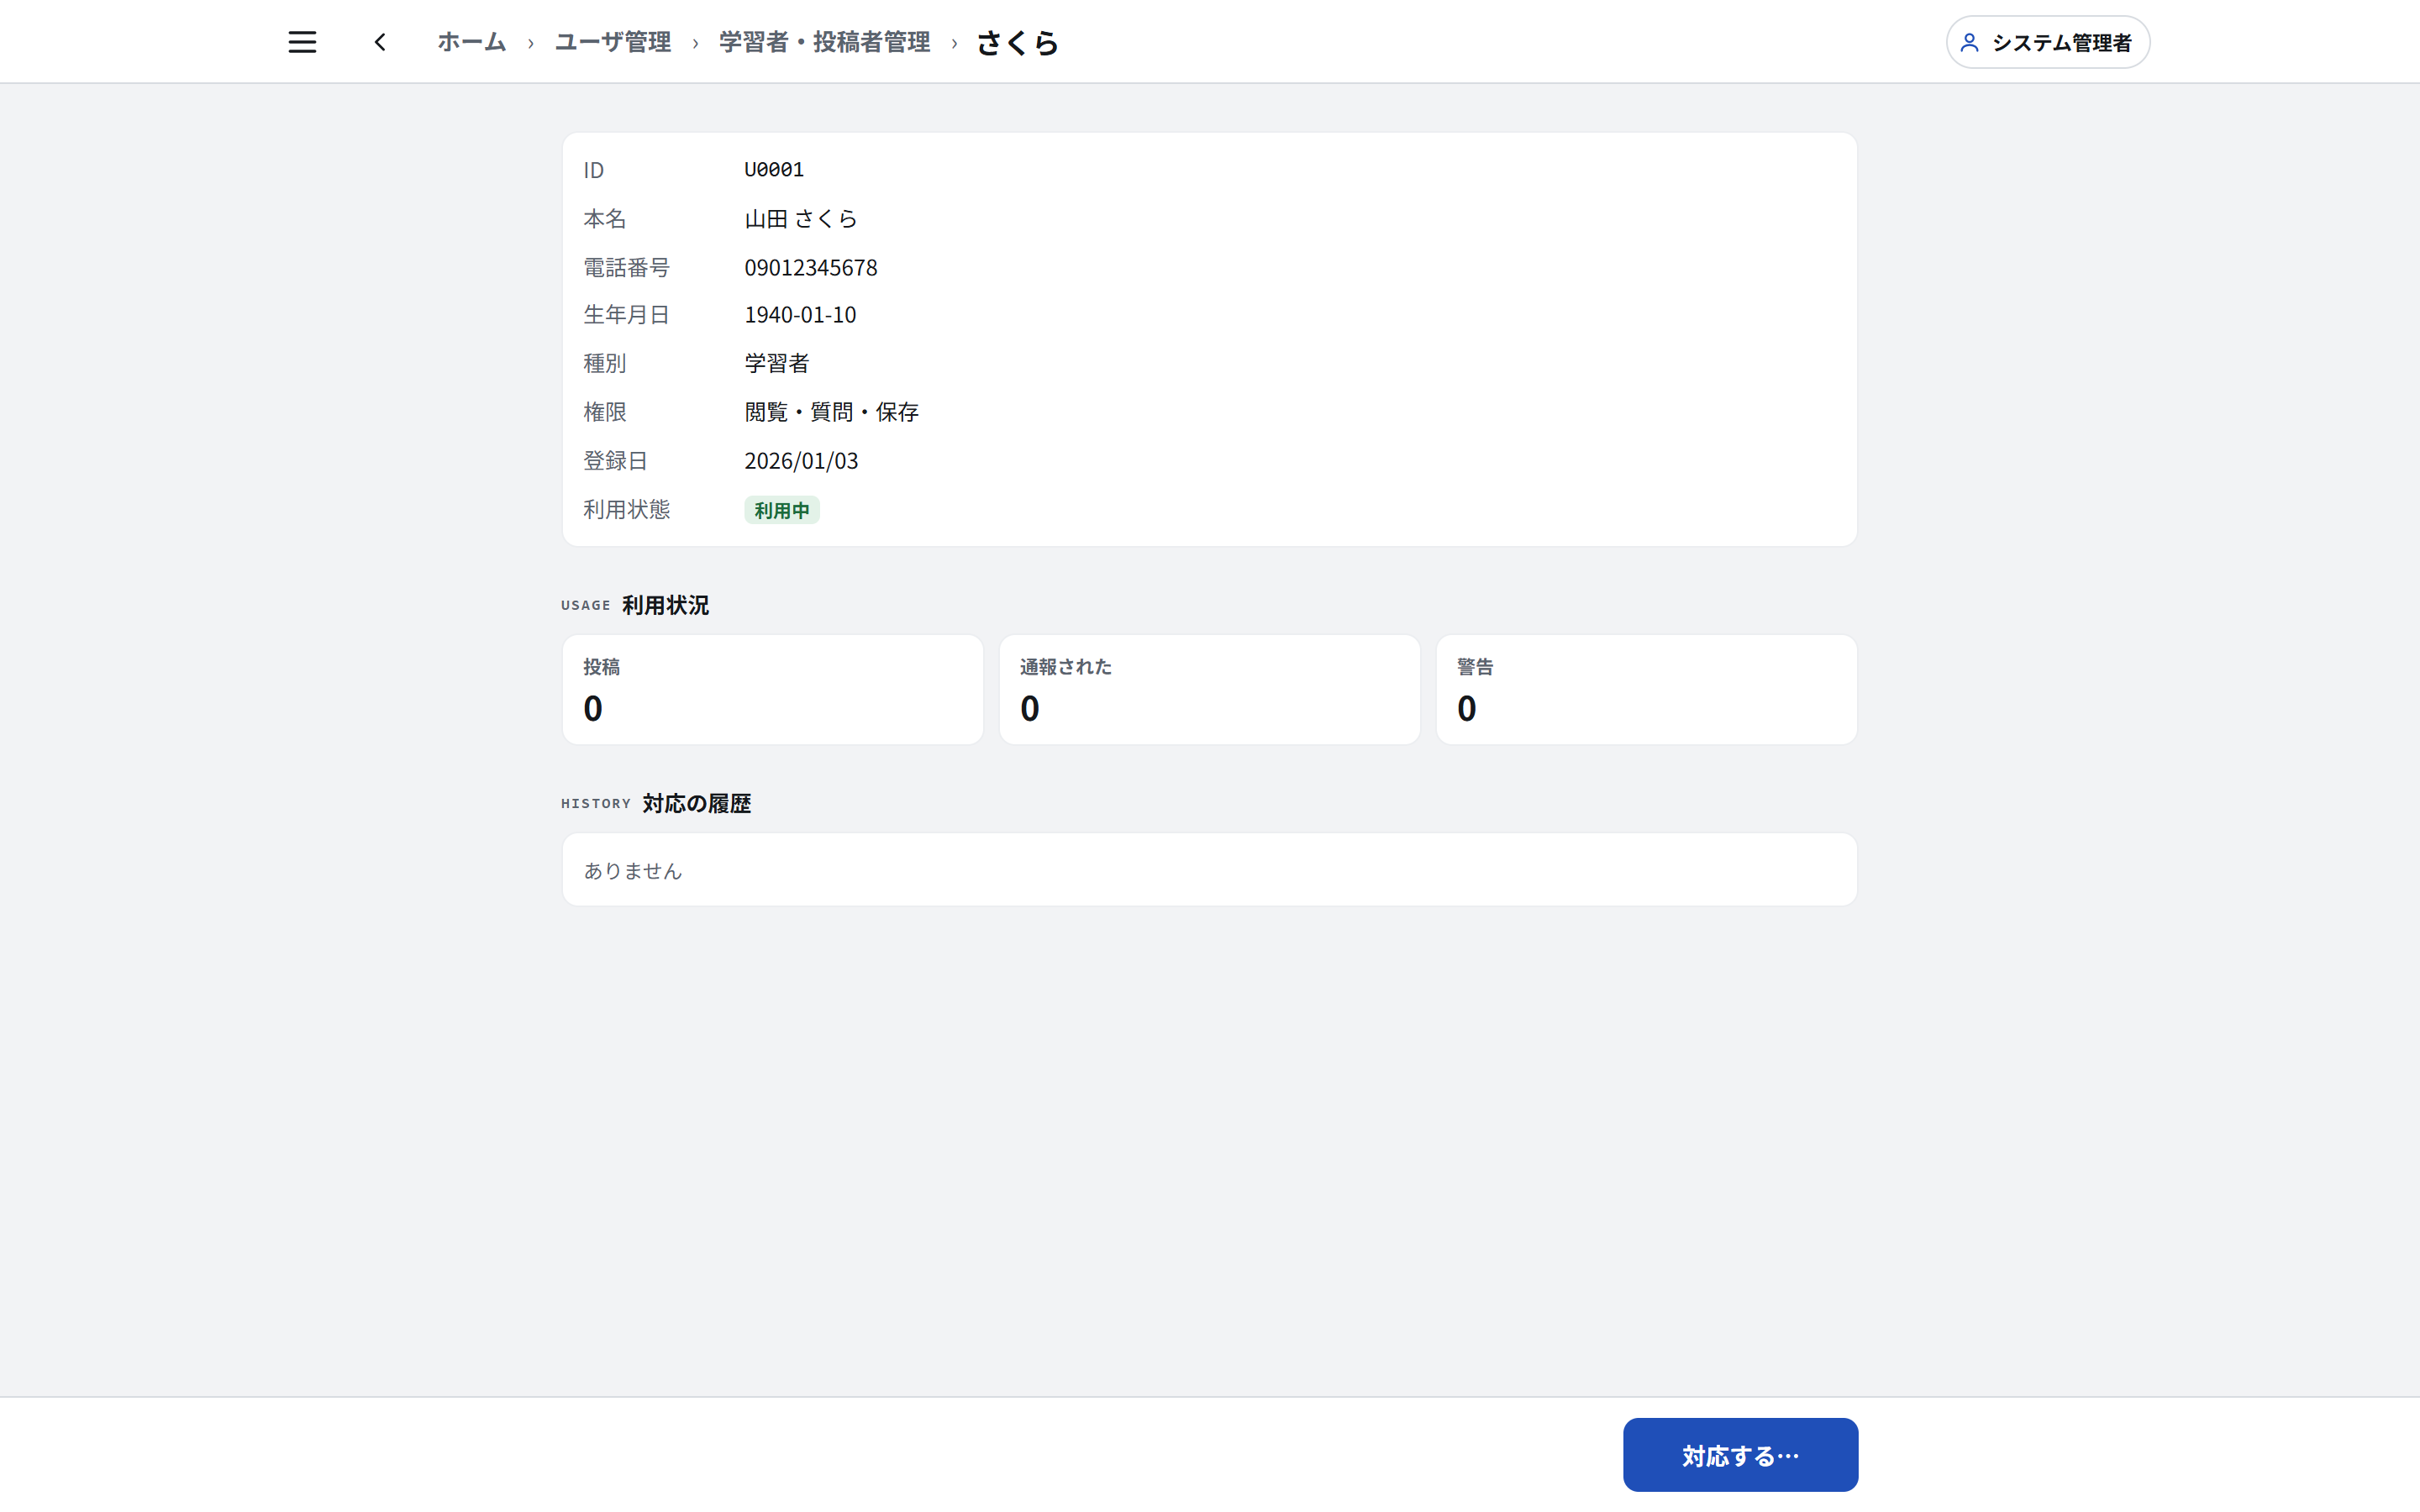
\includegraphics[width=\linewidth]{chapters/images/UI_Screen/admin/user_detail.png}
    \caption{利用者詳細画面}
    \label{fig:ad_user_detail}
  \end{subfigure}
  \hfill
  \begin{subfigure}[t]{0.48\linewidth}
    \centering
    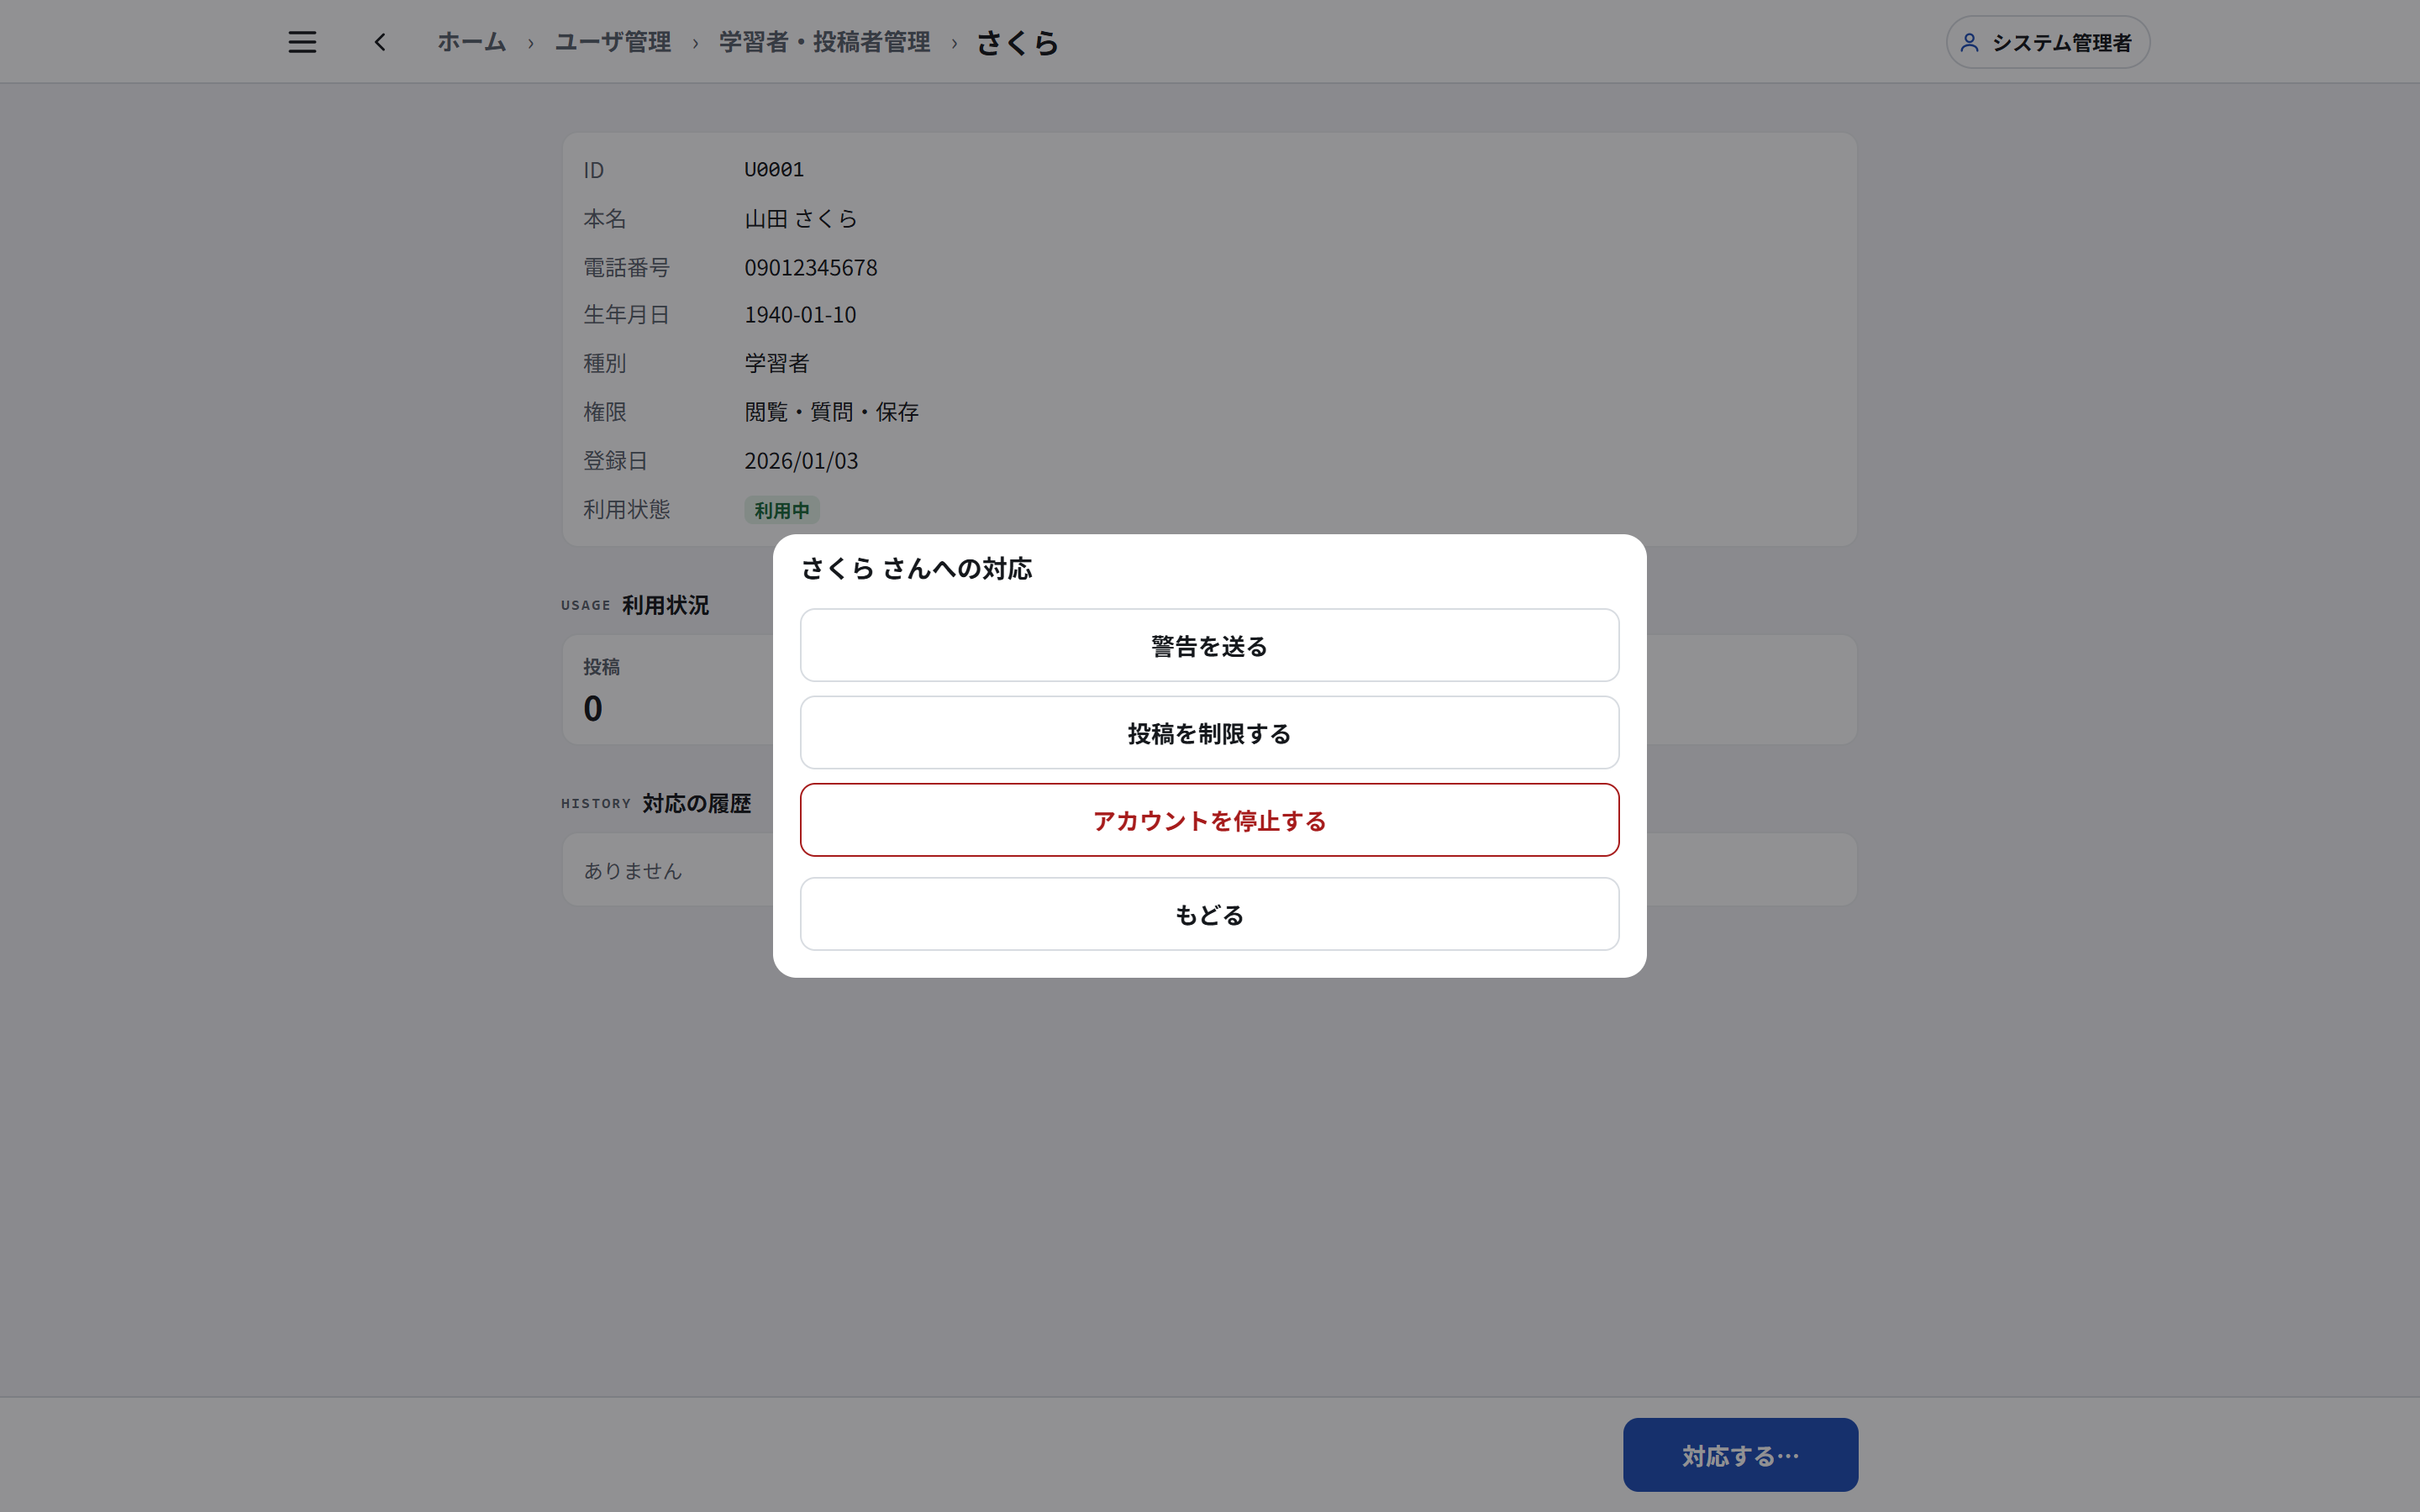
\includegraphics[width=\linewidth]{chapters/images/UI_Screen/admin/user_action.png}
    \caption{利用者への対応画面}
    \label{fig:ad_user_action}
  \end{subfigure}

  \caption{利用者詳細画面}
  \label{fig:ad_user_details}
\end{figure}

図\ref{fig:ad_user_detail}は、利用者1人の詳細情報を確認する画面である。ID・本名・電話番号・生年月日・種別・権限・登録日・利用状態と、投稿数・通報された数・警告の数、これまでの対応履歴が表示される。

図\ref{fig:ad_user_action}は、利用者詳細画面で「対応する…」をクリックすると表示される画面である。「警告を送る」「投稿を制限する」「アカウントを停止する」から対応を選択することができる。


\subsubsection{問い合わせ管理画面}

図\ref{fig:ad_inquiry}は、利用者から届いた問い合わせの一覧を確認する画面である。「未対応」「対応中」「対応済み」「すべて」で絞り込むことができる。一覧には内容・送った人・種類・受信日時・状態が表示され、行をクリックすると問い合わせ詳細画面へ遷移する。

\begin{figure}[H]
  \centering
  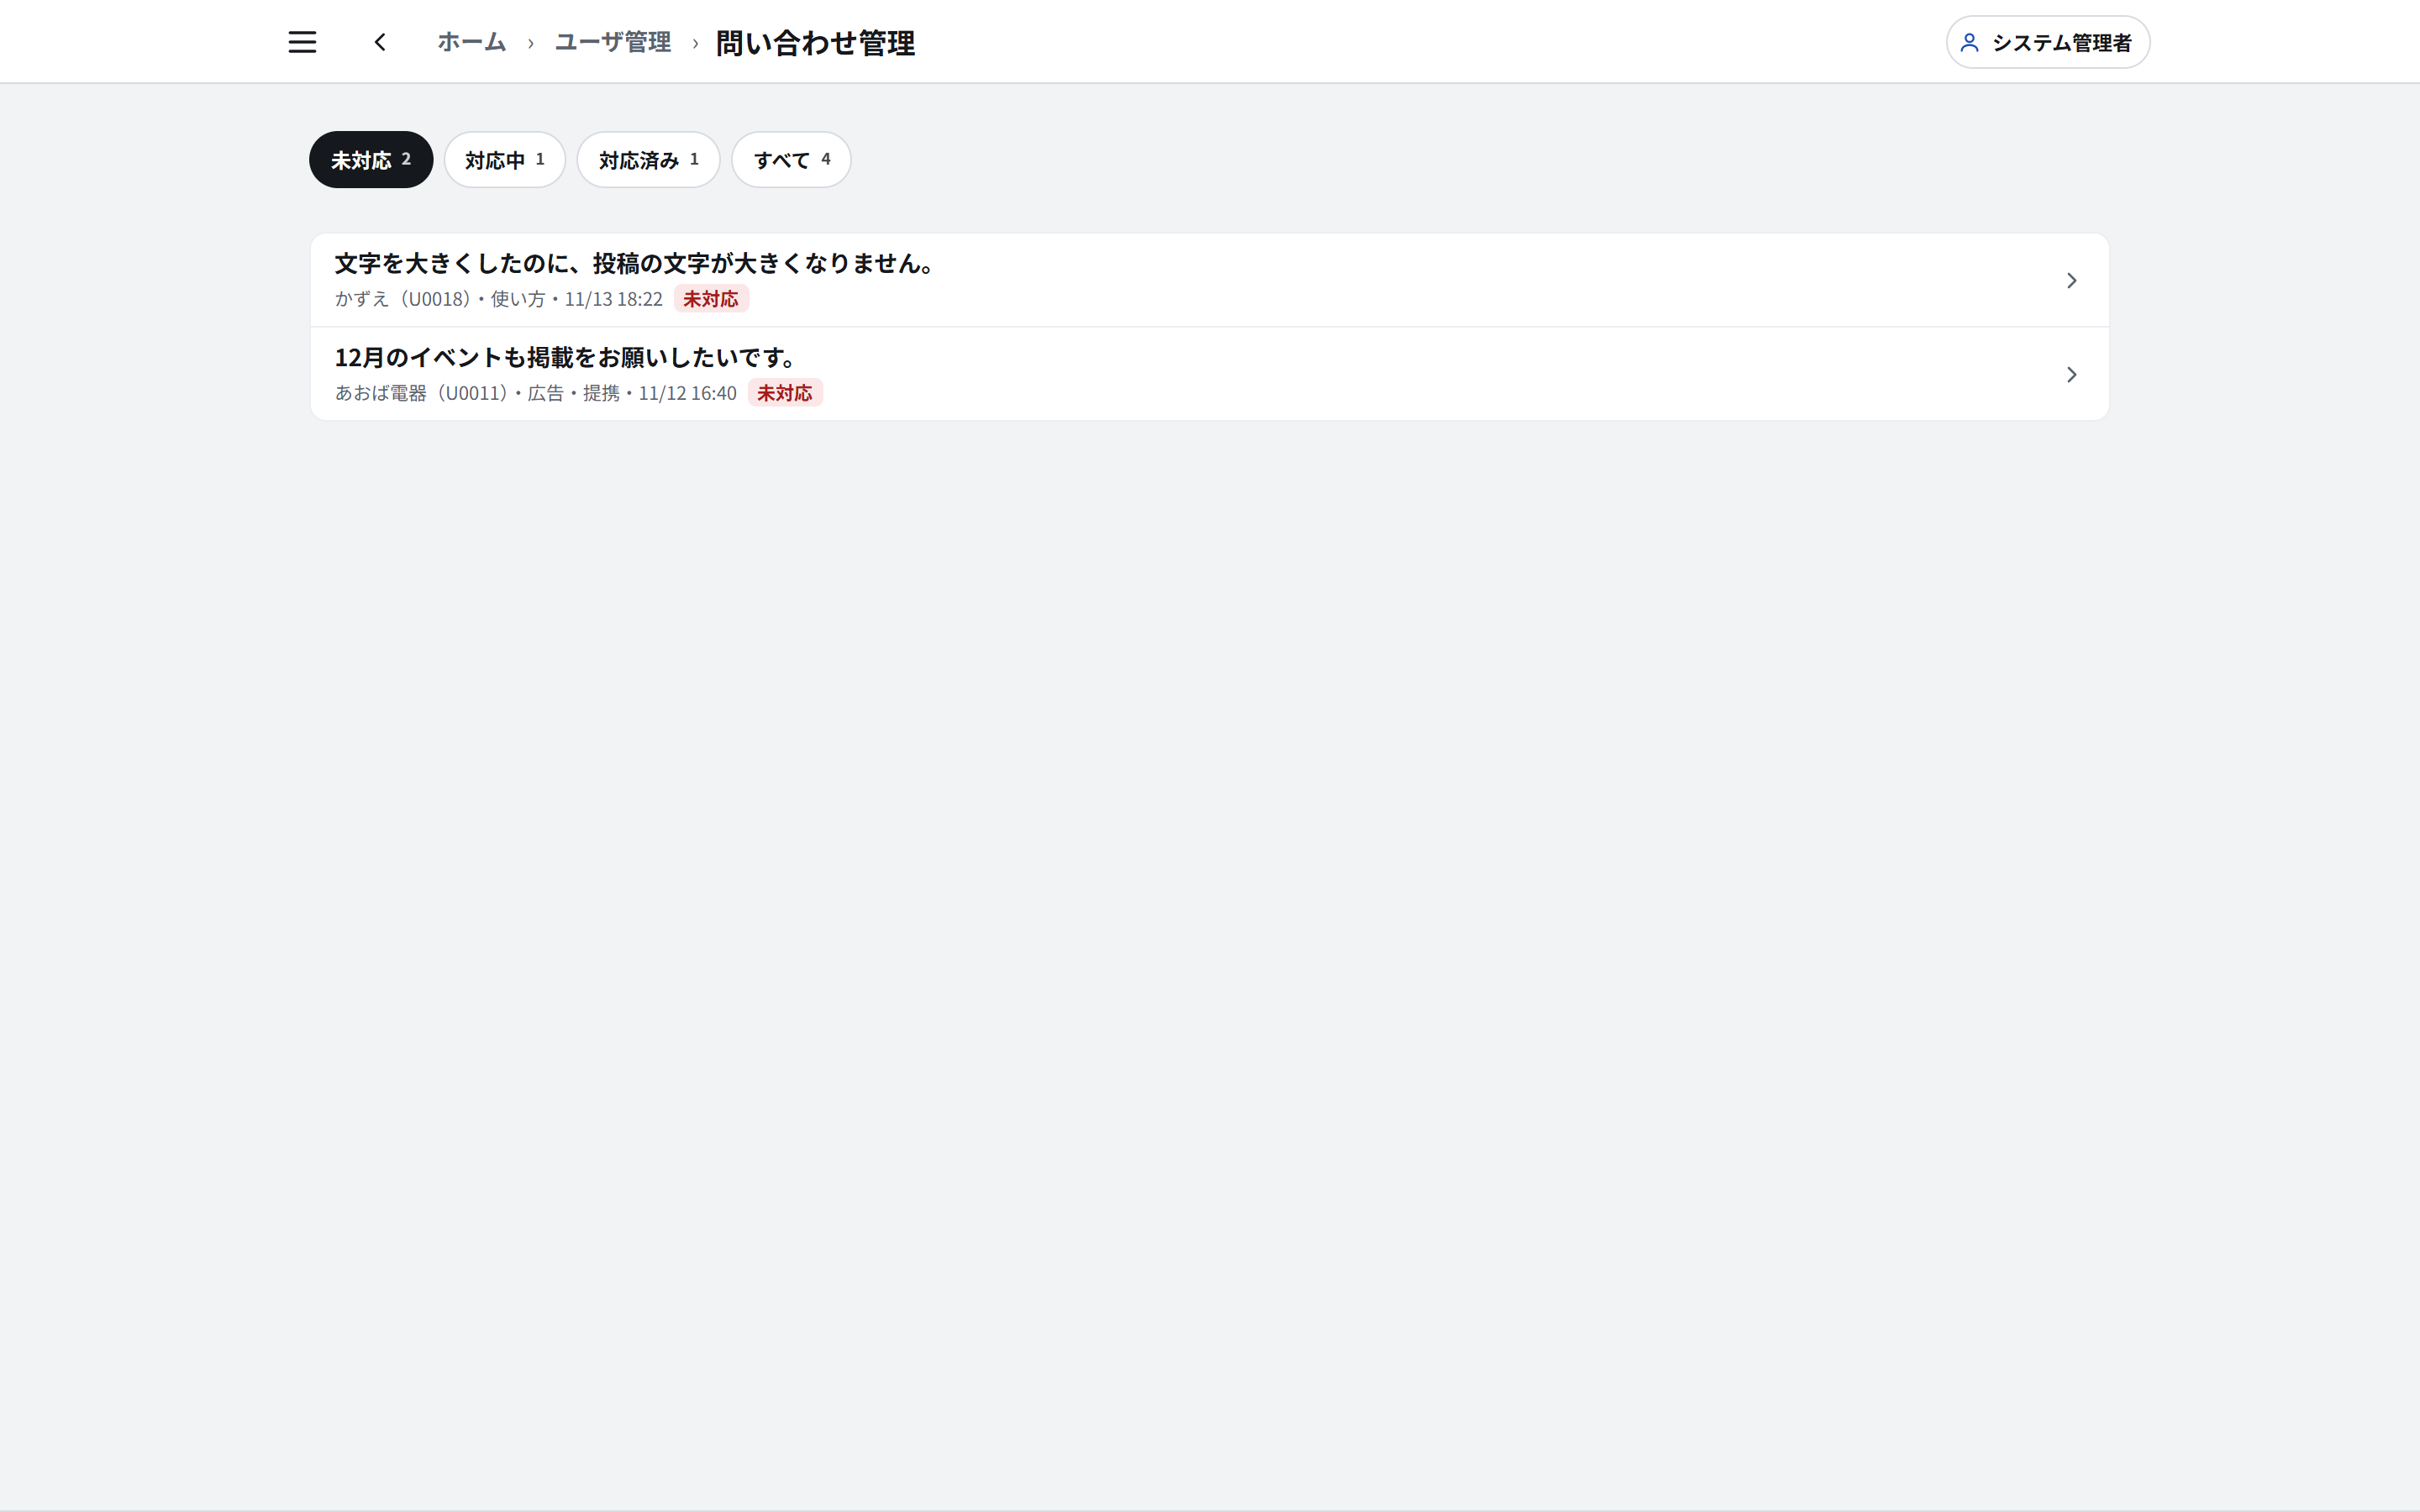
\includegraphics[width=\linewidth]{chapters/images/UI_Screen/admin/inquiry.png}
  \caption{問い合わせ管理画面}
  \label{fig:ad_inquiry}
\end{figure}


\subsubsection{問い合わせ詳細画面}

問い合わせ詳細画面を図\ref{fig:ad_inquiry_details}に示す。

\begin{figure}[H]
  \centering

  \begin{subfigure}[t]{0.48\linewidth}
    \centering
    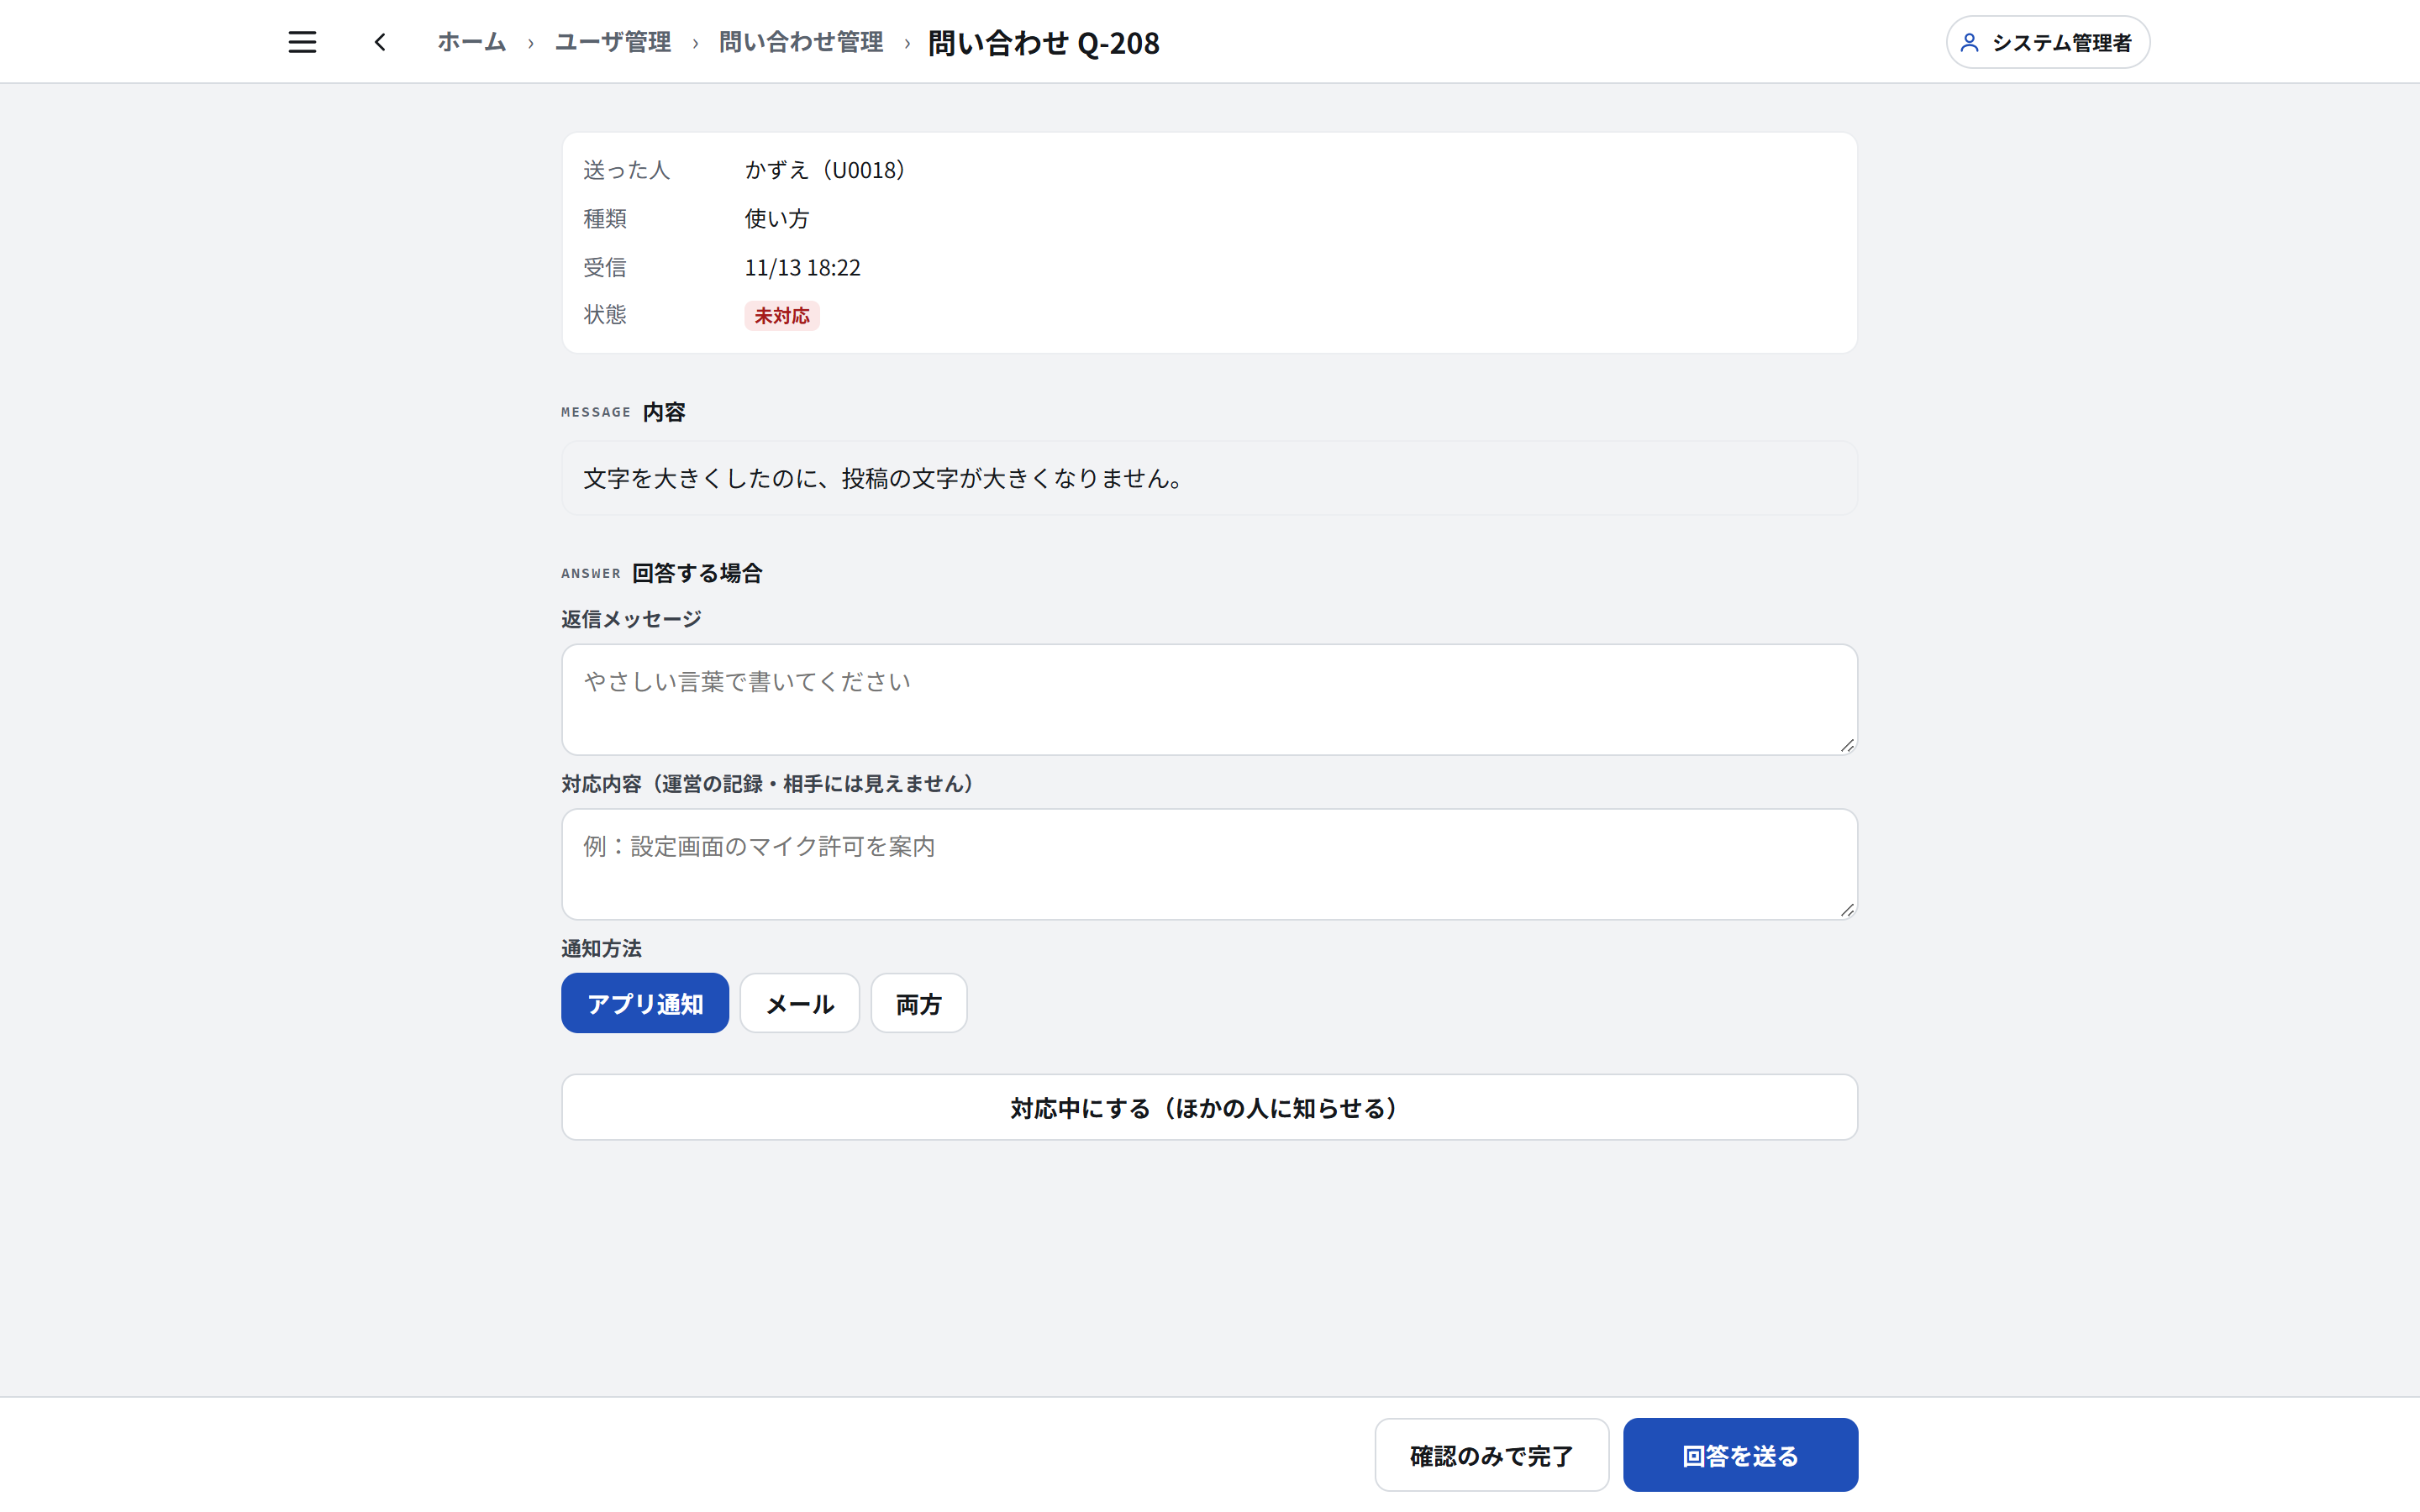
\includegraphics[width=\linewidth]{chapters/images/UI_Screen/admin/inquiry_detail.png}
    \caption{問い合わせ詳細画面}
    \label{fig:ad_inquiry_detail}
  \end{subfigure}
  \hfill
  \begin{subfigure}[t]{0.48\linewidth}
    \centering
    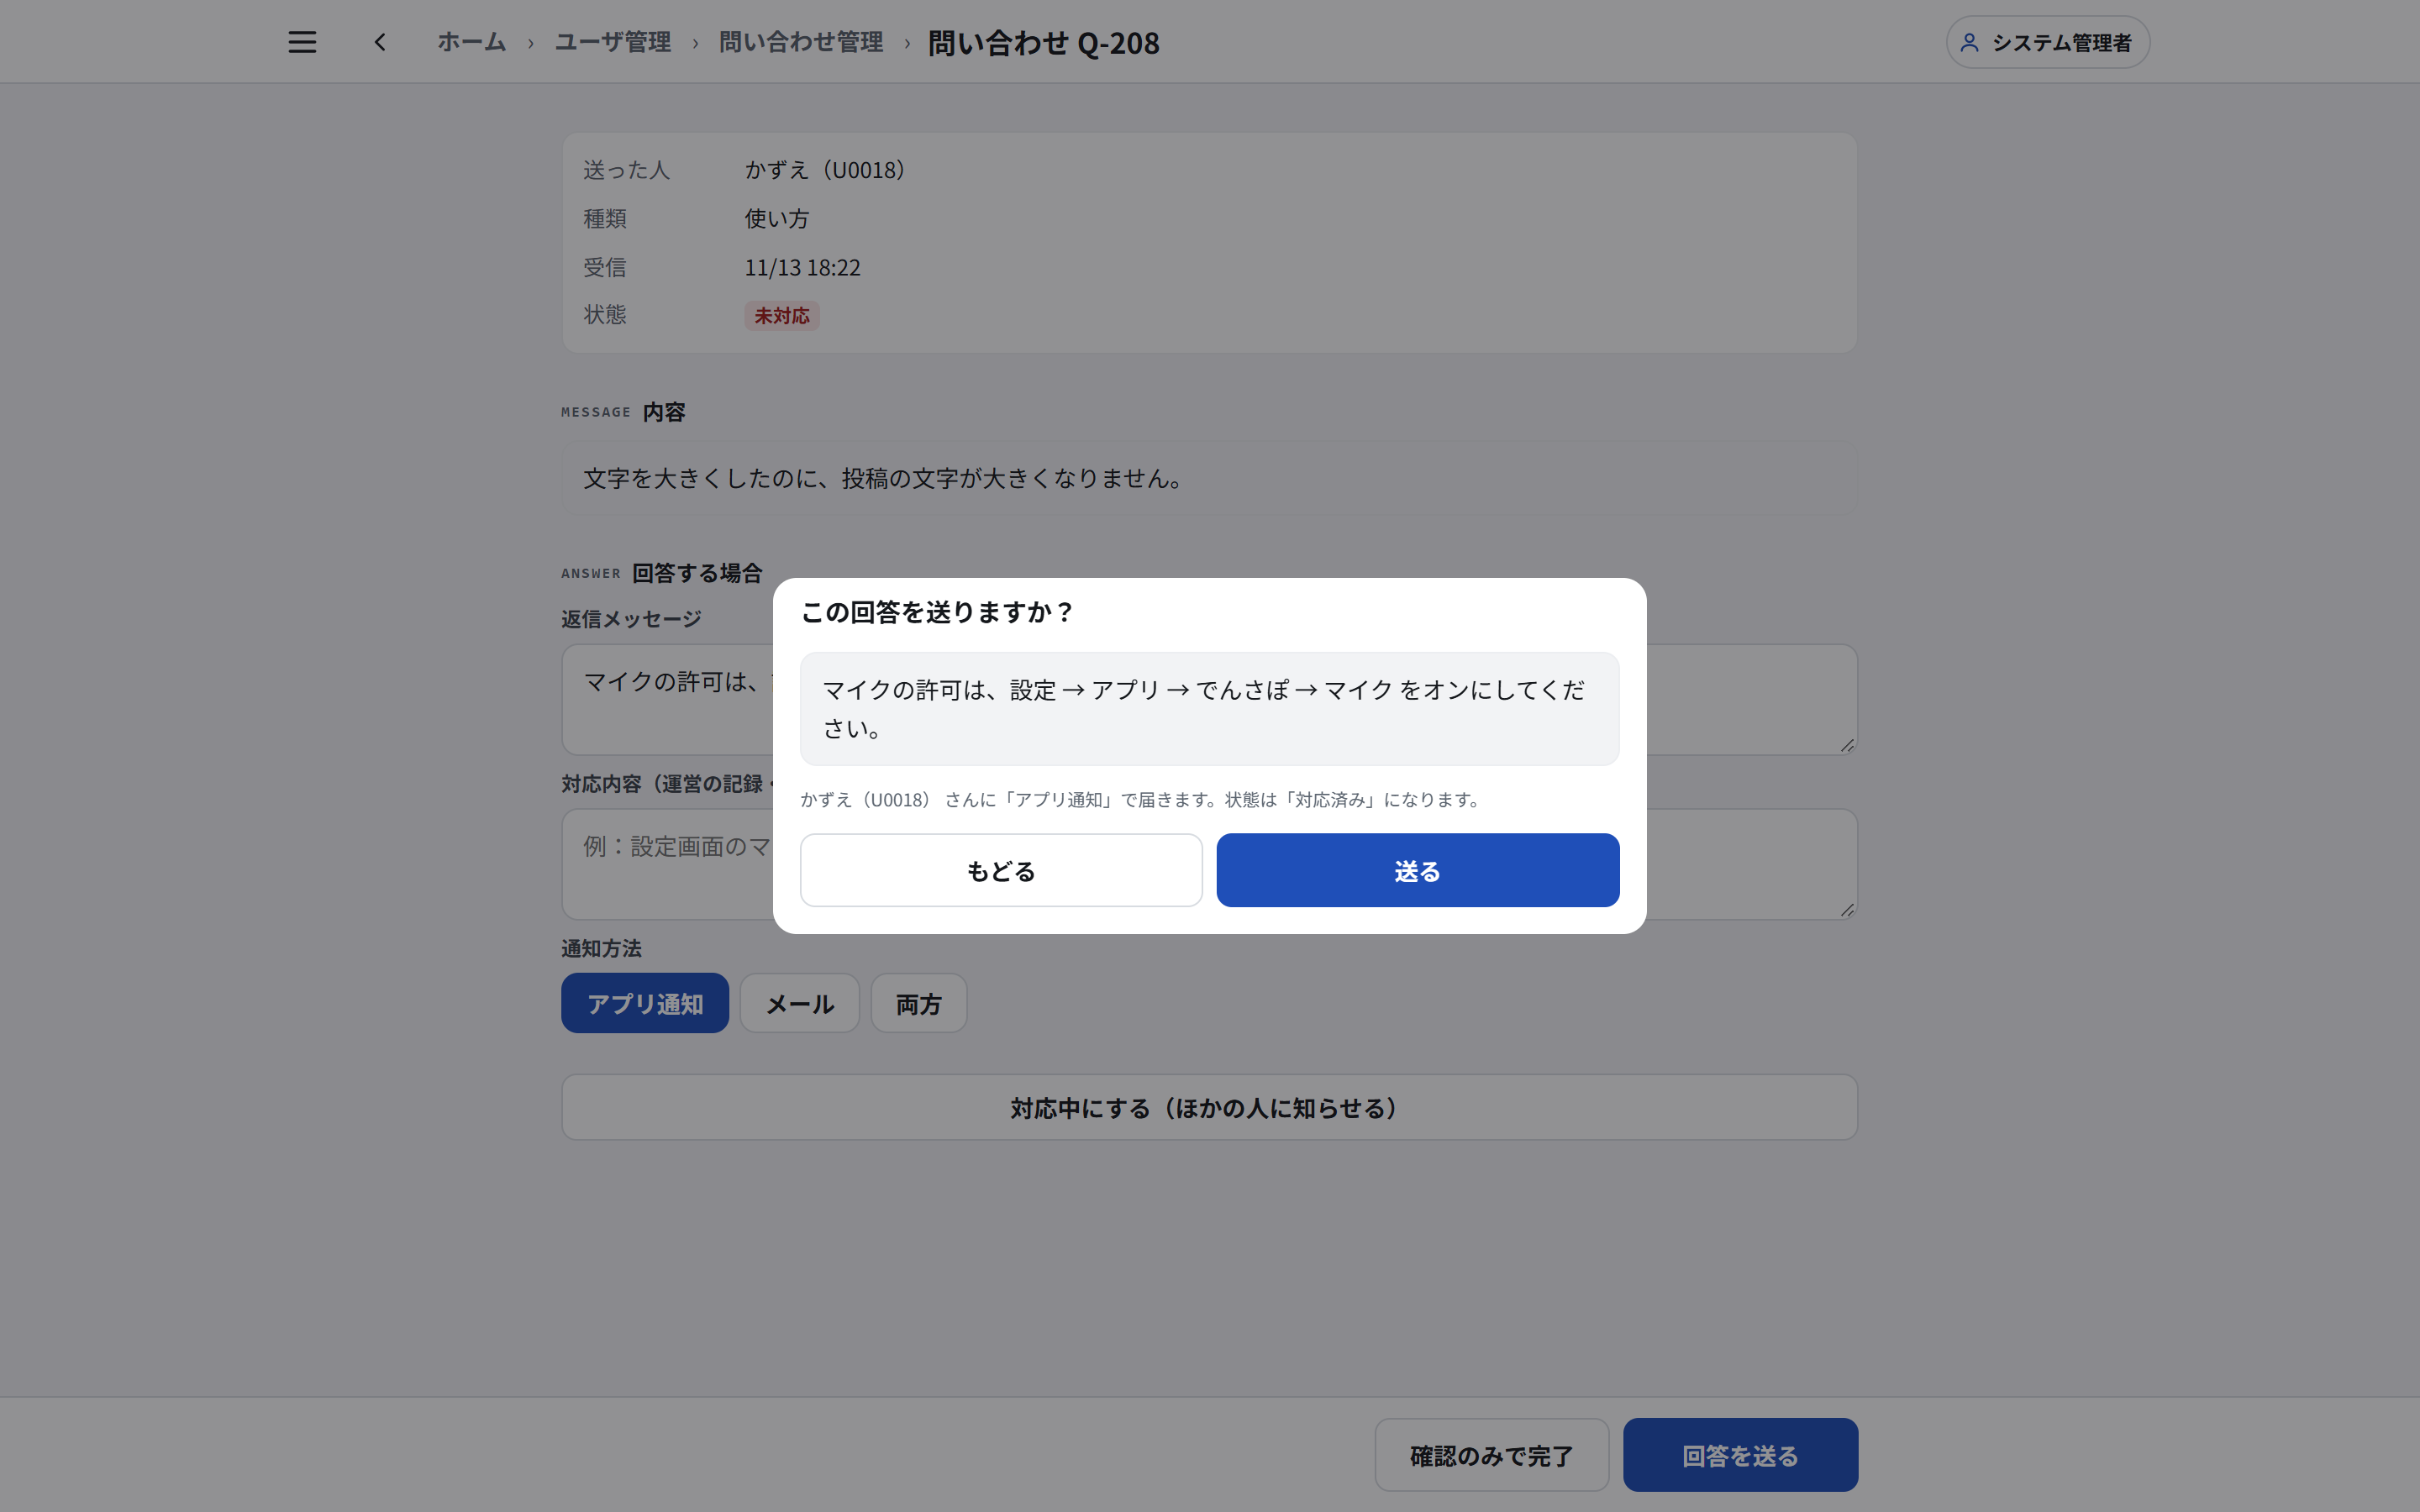
\includegraphics[width=\linewidth]{chapters/images/UI_Screen/admin/inquiry_send.png}
    \caption{回答の確認画面}
    \label{fig:ad_inquiry_send}
  \end{subfigure}

  \caption{問い合わせ詳細画面}
  \label{fig:ad_inquiry_details}
\end{figure}

図\ref{fig:ad_inquiry_detail}は、問い合わせ1件の内容を確認し、回答する画面である。送った人・種類・受信日時・状態と、問い合わせの内容が表示される。返信メッセージ、運営のみが閲覧できる対応内容の記録、通知方法（アプリ通知・メール・両方）を入力し、「回答を送る」をクリックすると回答できる。回答が不要な場合は「確認のみで完了」をクリックする。また、「対応中にする」をクリックすると、ほかの管理者に対応中であることを知らせることができる。

図\ref{fig:ad_inquiry_send}は、「回答を送る」をクリックすると表示される確認画面である。送る内容と送る相手、通知方法が表示される。「送る」をクリックすると回答が届き、問い合わせの状態が「対応済み」になる。


% =================================
\subsection{投稿管理画面}
% =================================

\subsubsection{投稿管理（パネル一覧）画面}

図\ref{fig:ad_post_panel}は、ホーム画面で「投稿管理」をクリックすると表示される画面である。「投稿管理」と「通報管理」のパネルが配置され、未対応がある場合は件数が表示される。クリックするとそれぞれの画面へ遷移する。

\begin{figure}[H]
  \centering
  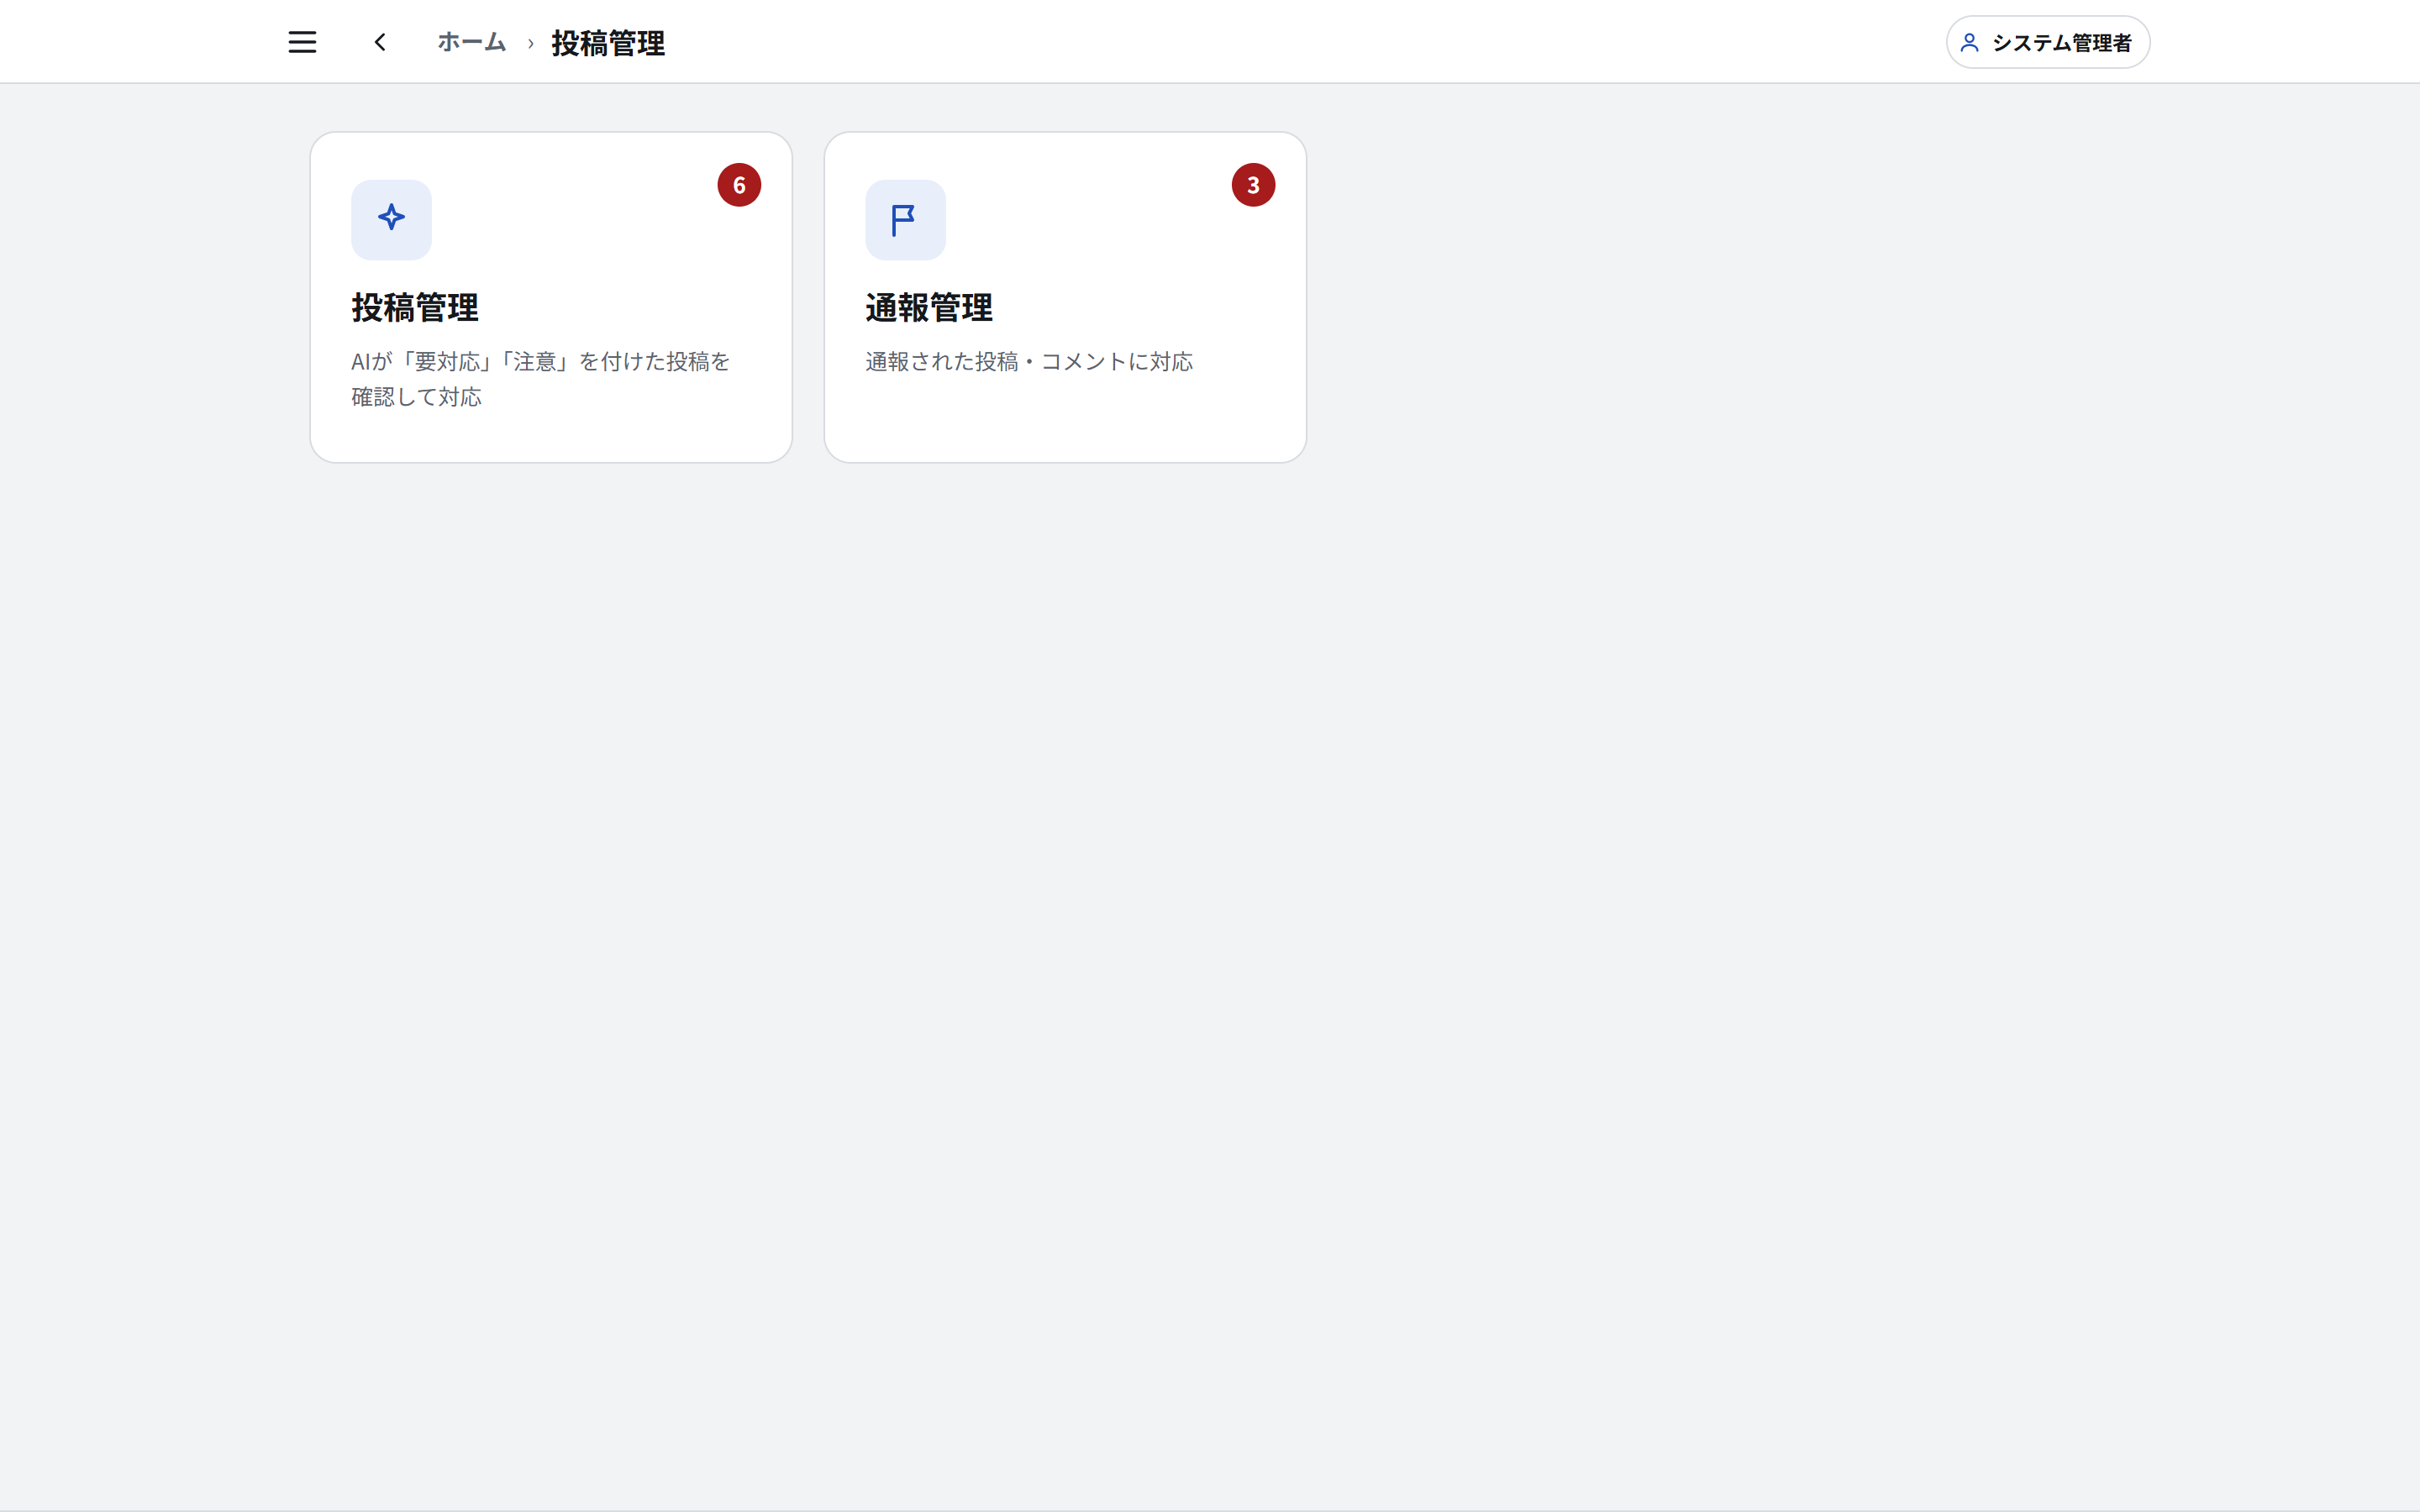
\includegraphics[width=\linewidth]{chapters/images/UI_Screen/admin/post_panel.png}
  \caption{投稿管理（パネル一覧）画面}
  \label{fig:ad_post_panel}
\end{figure}


\subsubsection{投稿管理画面}

図\ref{fig:ad_post}は、投稿の一覧を確認する画面である。投稿は審査なしで公開され、AIがすべての投稿を解析し、不適切な内容やキーワードにタグを付ける。「要対応」「注意」「確認」「確認済み」「すべて」で絞り込むことができる。一覧には投稿のタイトル・ID・AIの判定とその理由・投稿者・日時・通報数が表示され、行をクリックすると投稿詳細画面へ遷移する。

\begin{figure}[H]
  \centering
  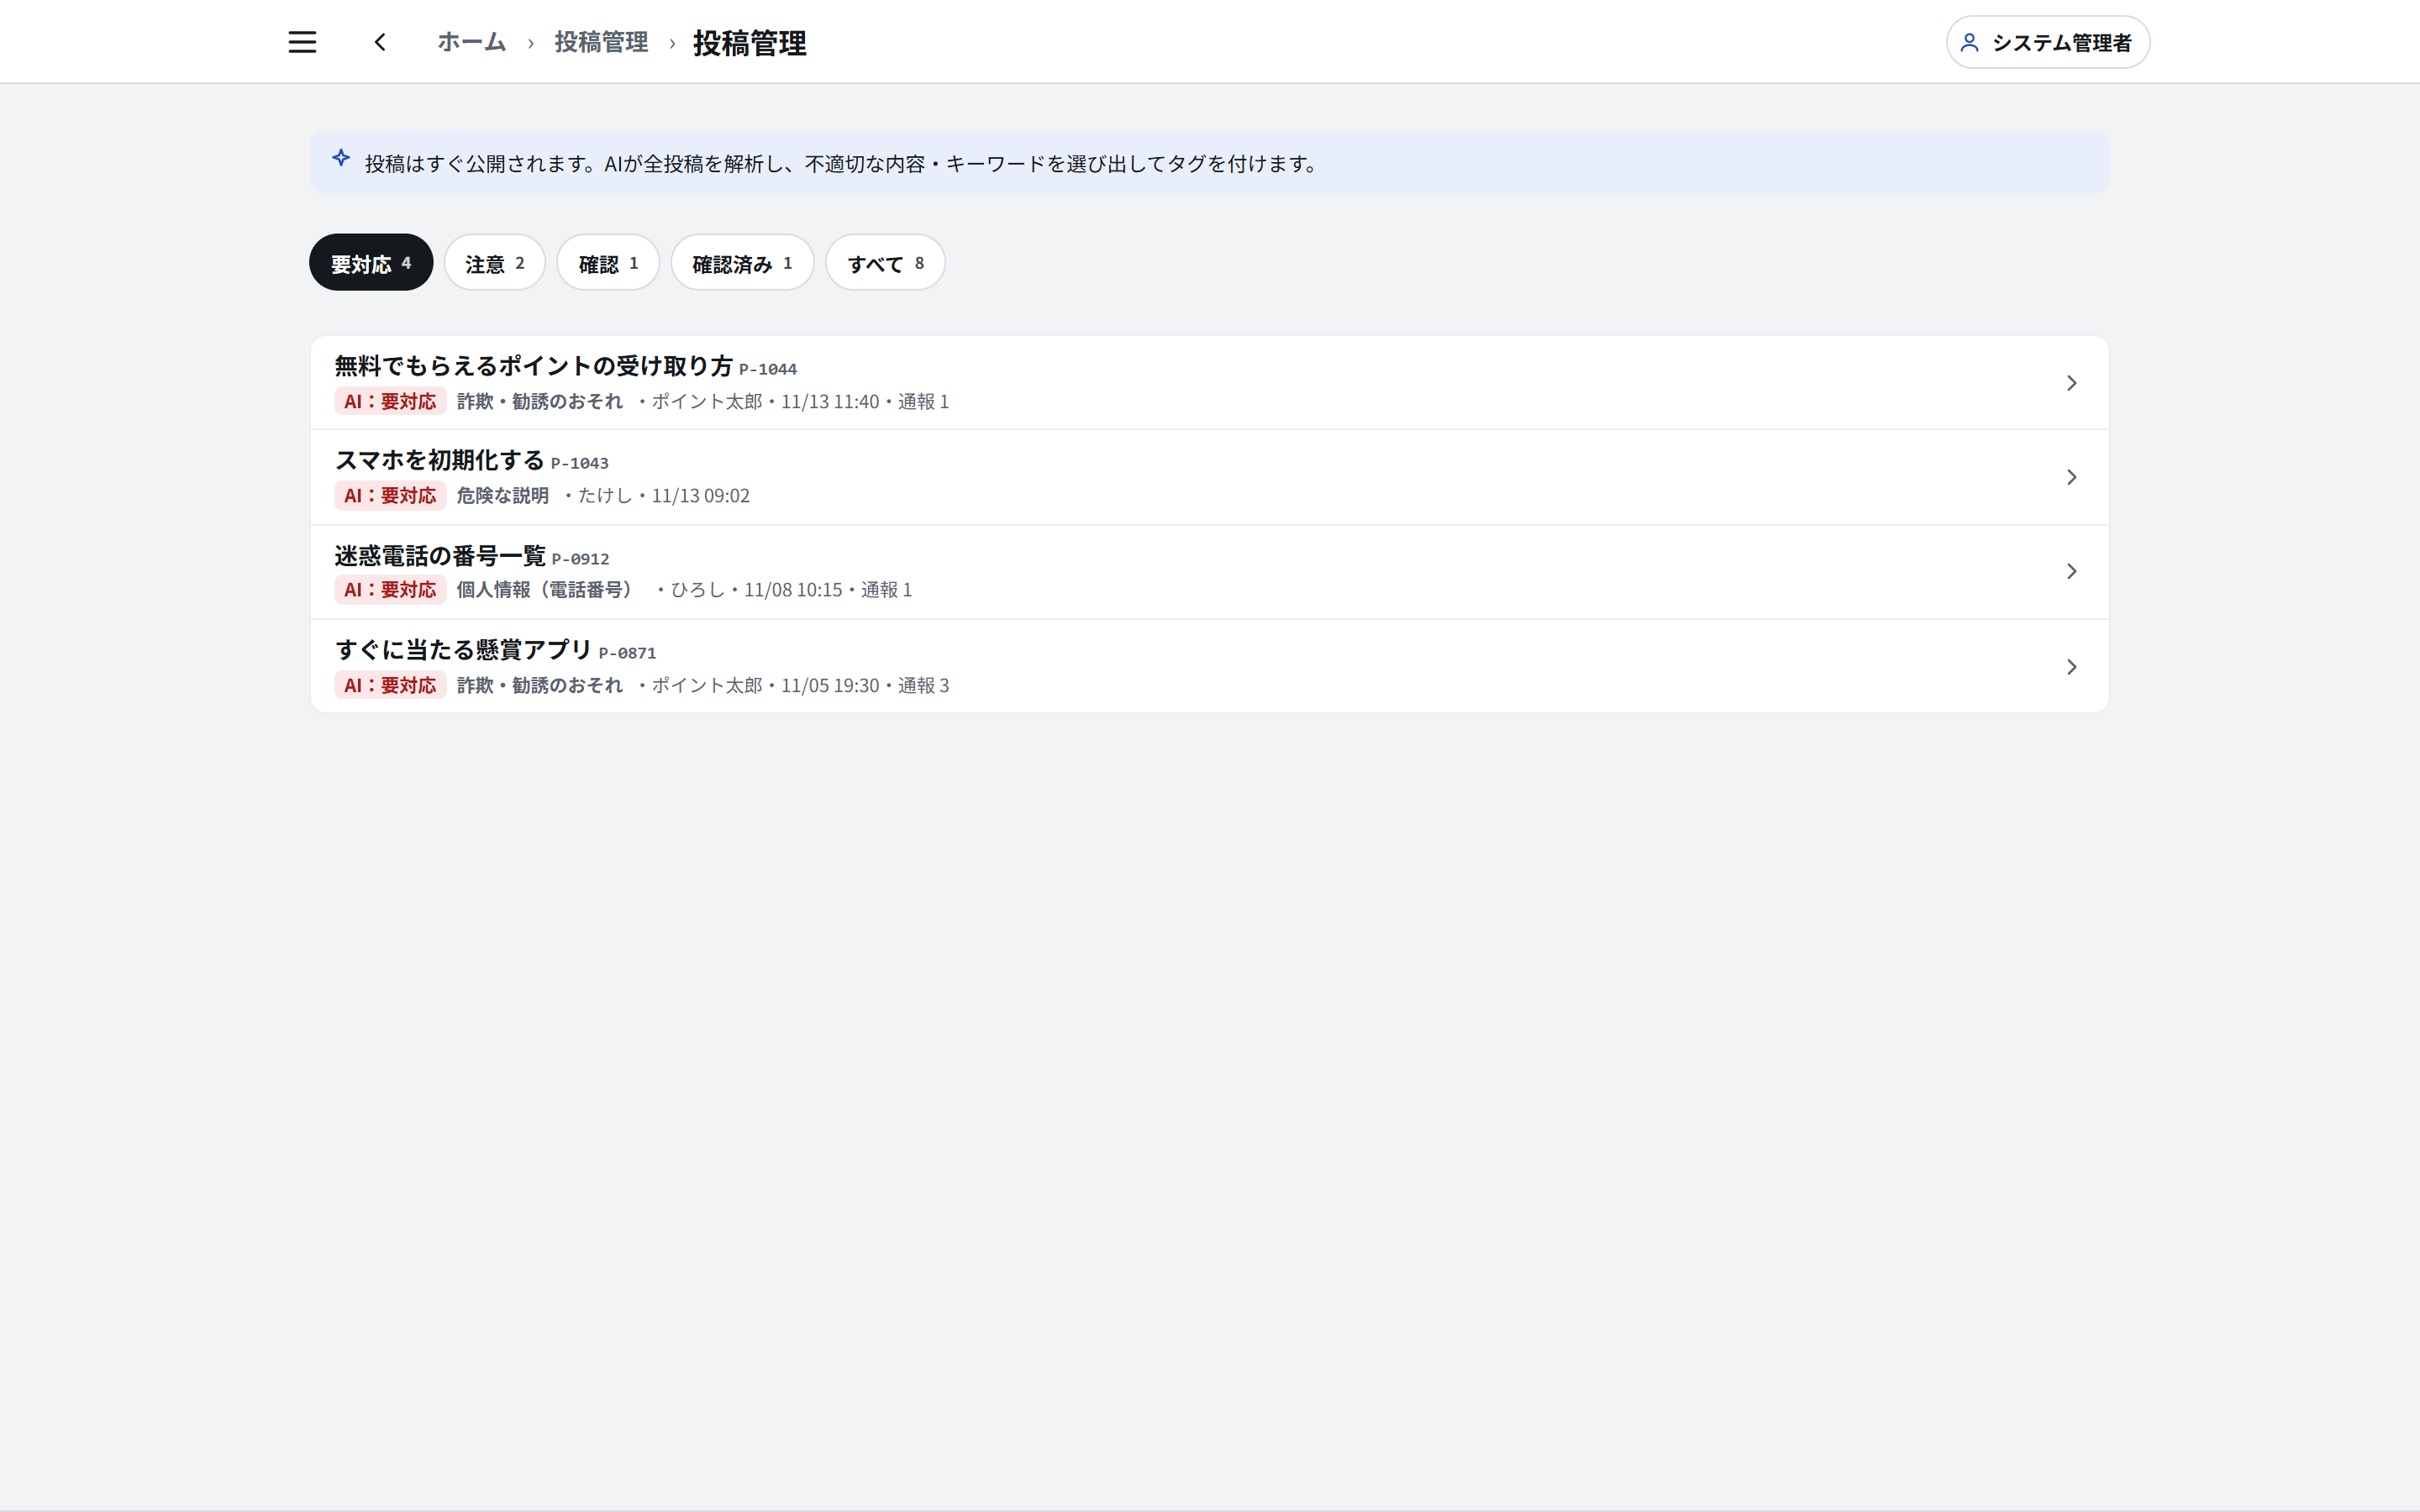
\includegraphics[width=\linewidth]{chapters/images/UI_Screen/admin/post.png}
  \caption{投稿管理画面}
  \label{fig:ad_post}
\end{figure}


\subsubsection{投稿詳細画面}

投稿詳細画面を図\ref{fig:ad_post_details}に示す。

\begin{figure}[H]
  \centering

  \begin{subfigure}[t]{0.48\linewidth}
    \centering
    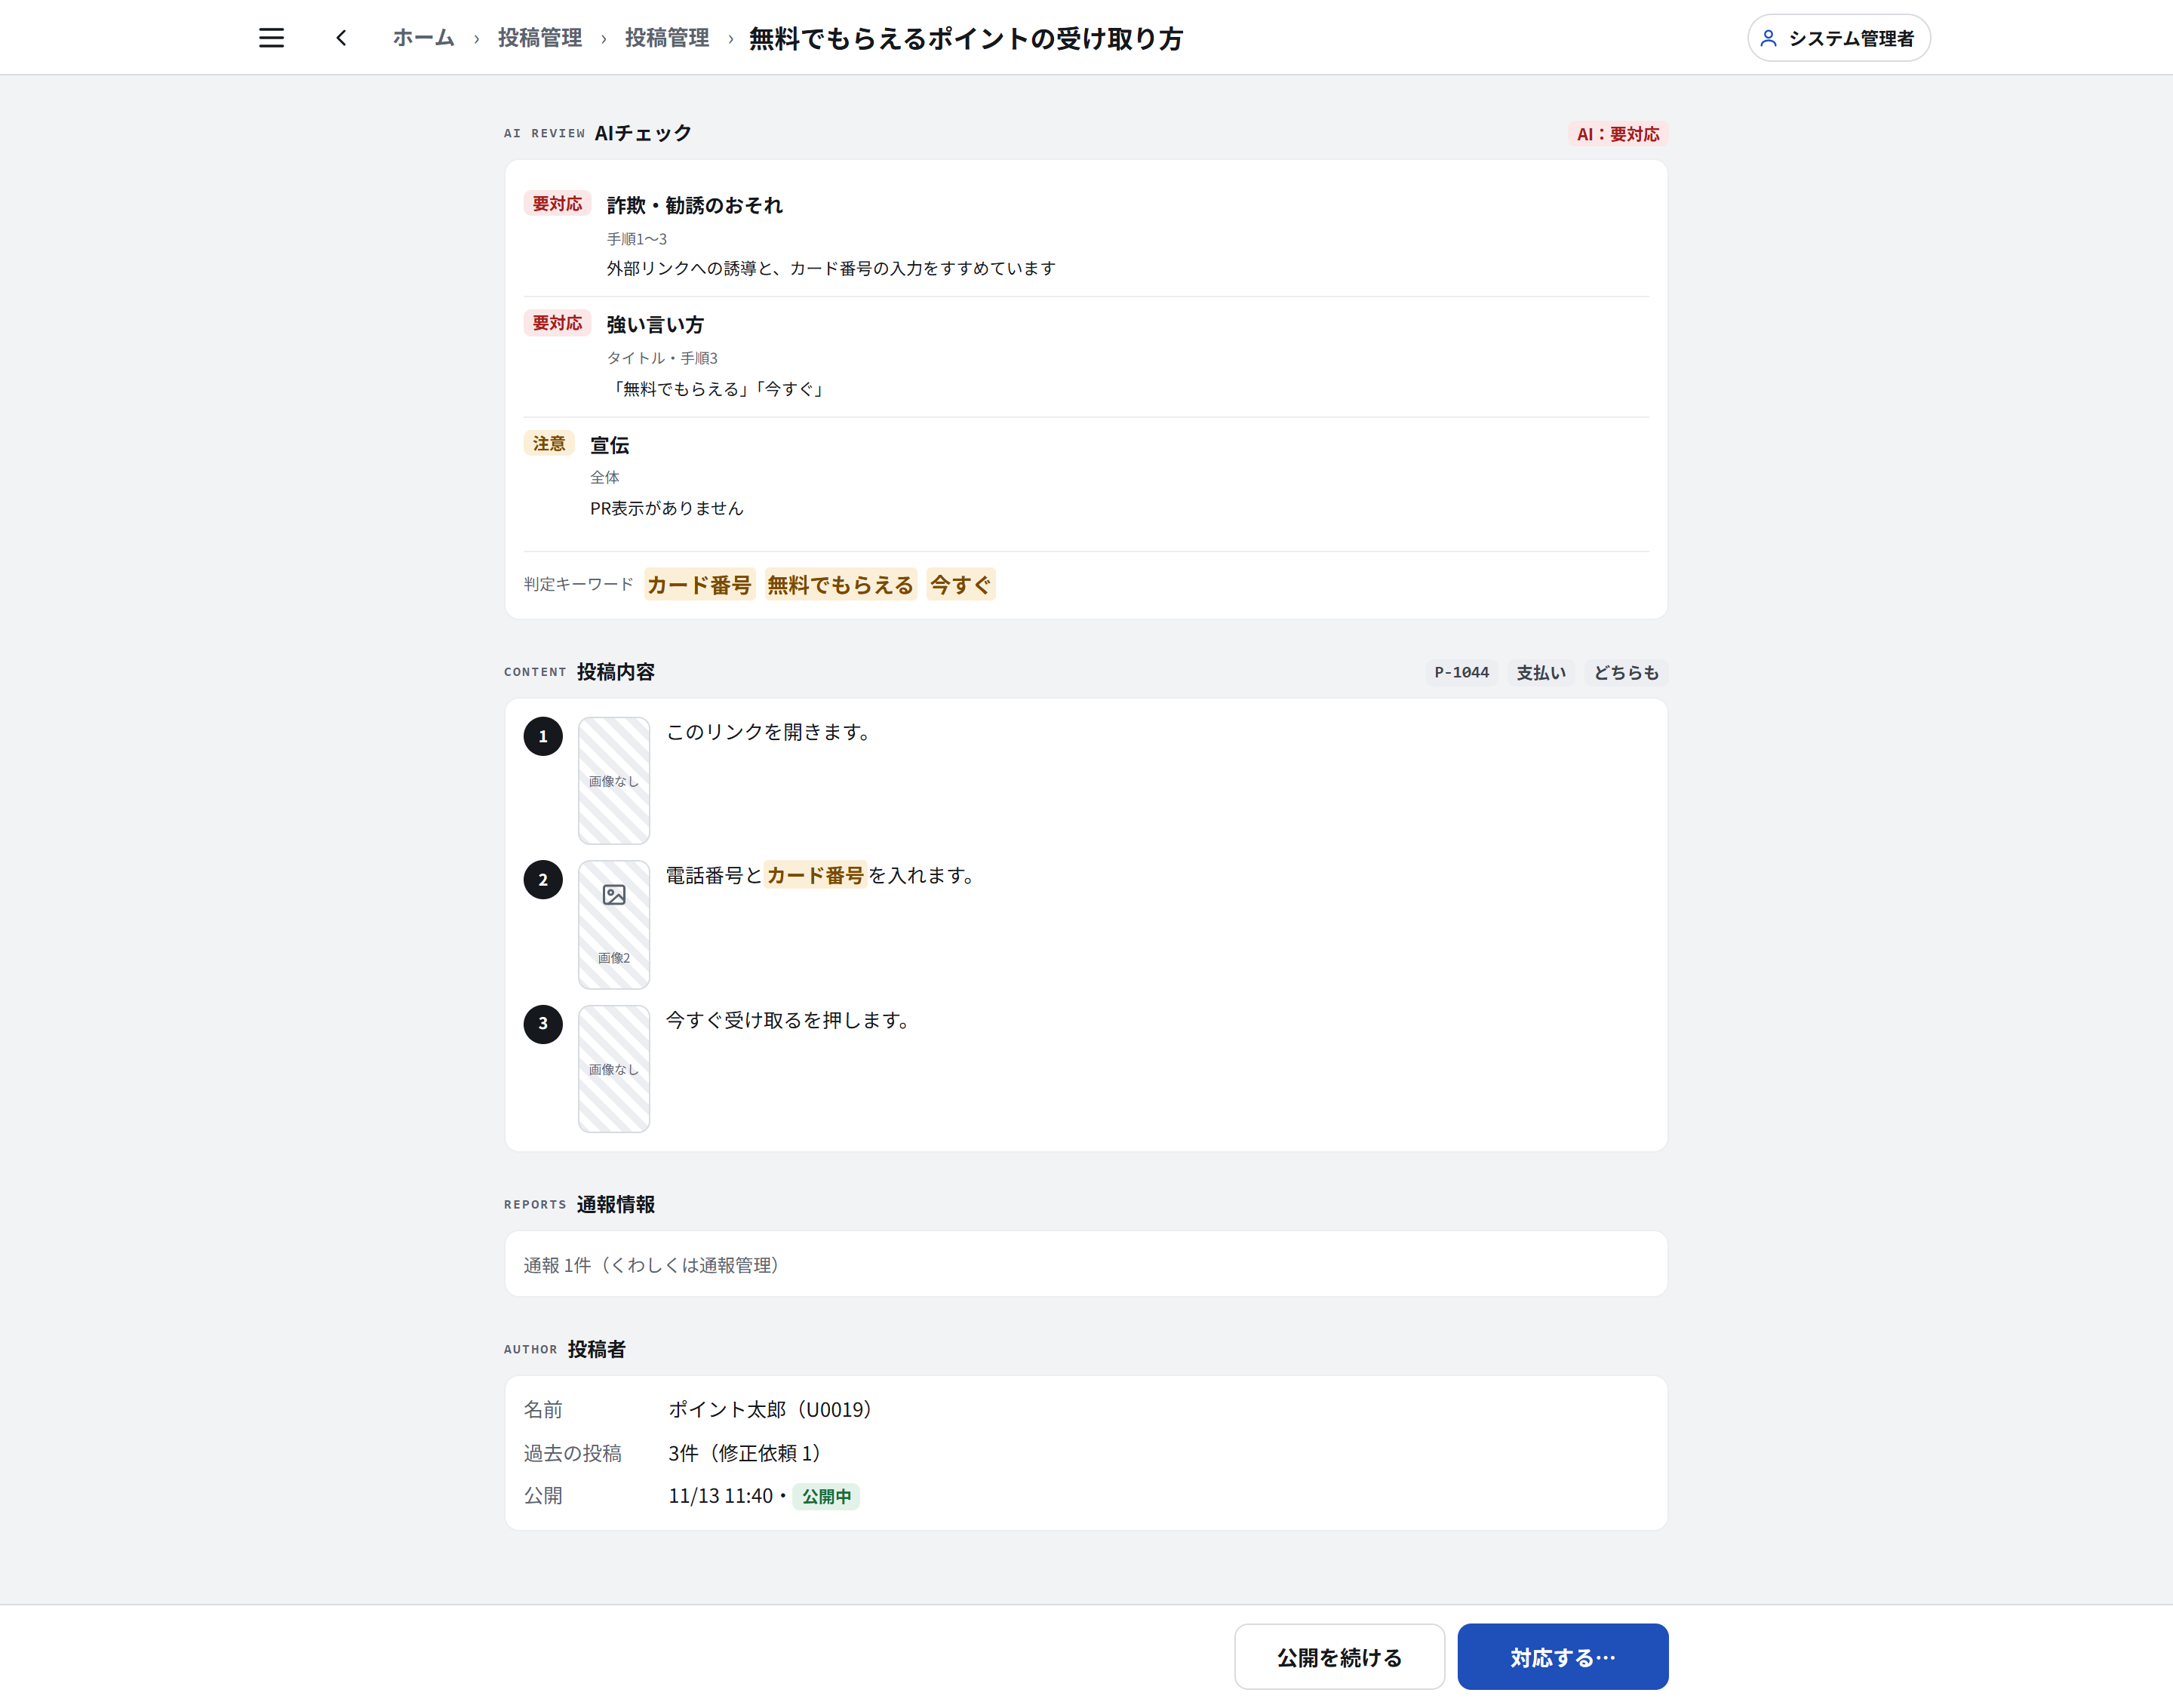
\includegraphics[width=\linewidth]{chapters/images/UI_Screen/admin/post_detail.png}
    \caption{投稿詳細画面}
    \label{fig:ad_post_detail}
  \end{subfigure}
  \hfill
  \begin{subfigure}[t]{0.48\linewidth}
    \centering
    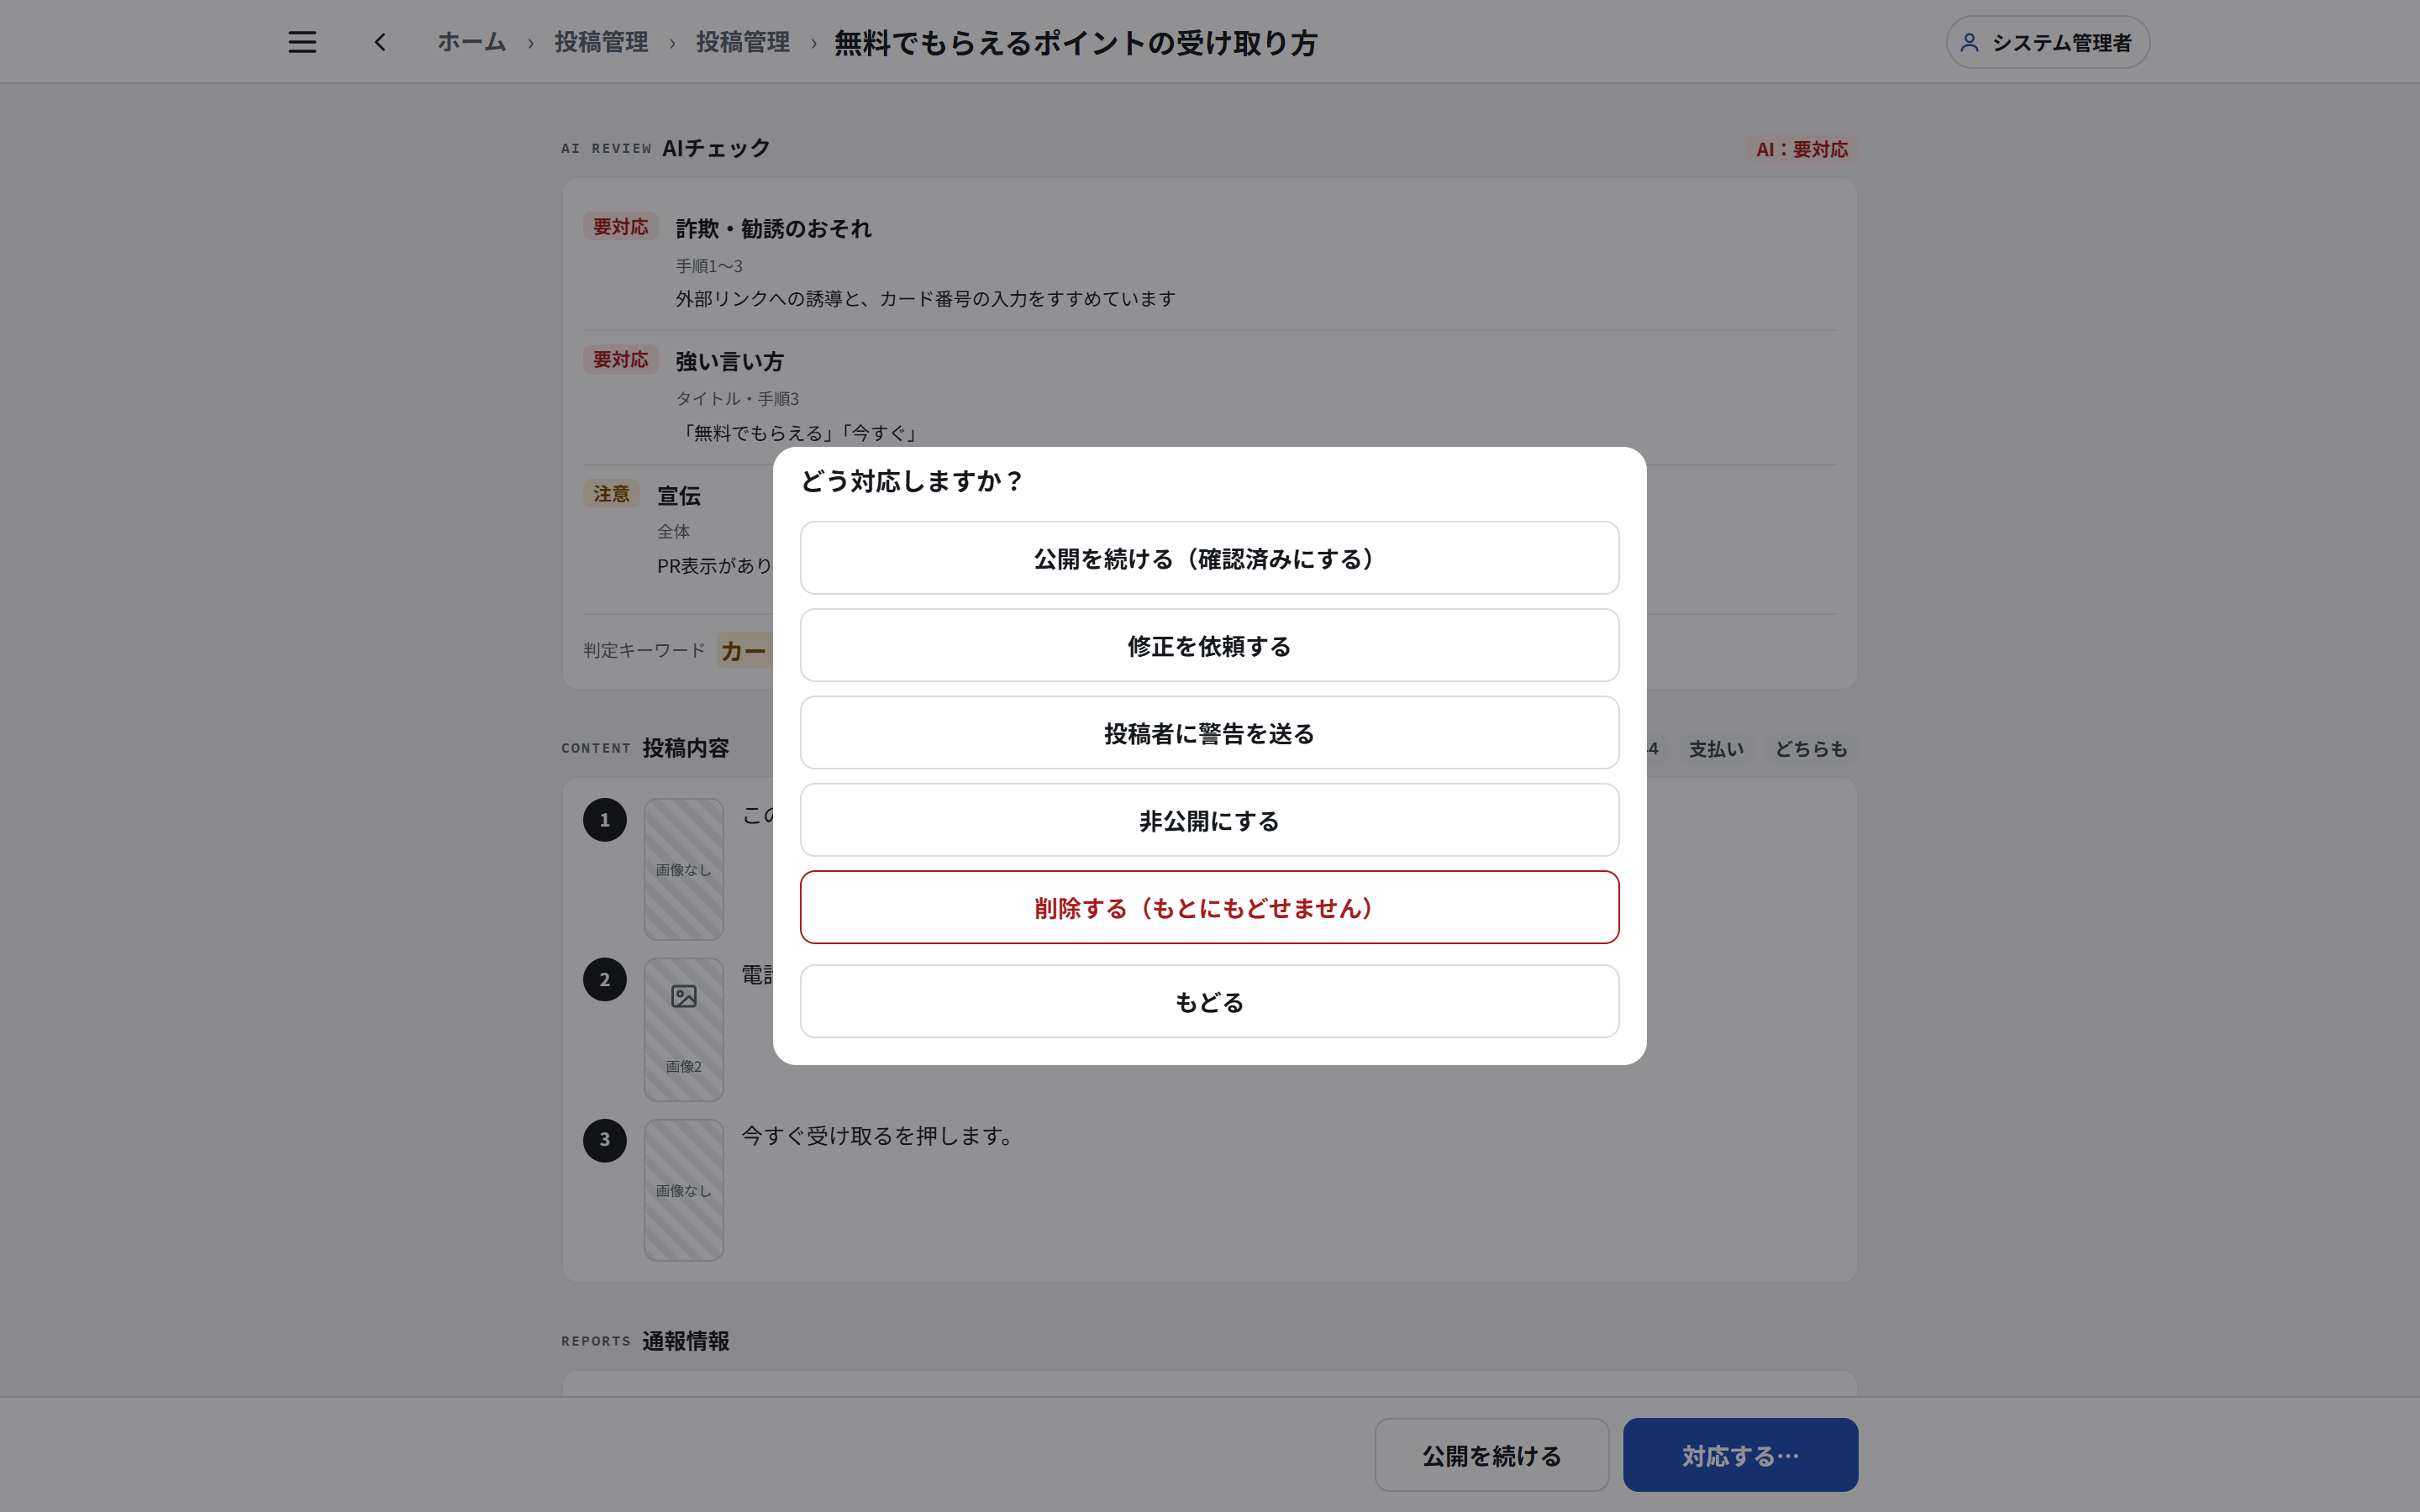
\includegraphics[width=\linewidth]{chapters/images/UI_Screen/admin/post_action.png}
    \caption{投稿への対応画面}
    \label{fig:ad_post_action}
  \end{subfigure}

  \caption{投稿詳細画面}
  \label{fig:ad_post_details}
\end{figure}

図\ref{fig:ad_post_detail}は、投稿1件の内容とAIの判定を確認する画面である。AIチェック欄には、指摘ごとのレベル・場所・内容と判定キーワードが表示される。投稿内容では、問題のある言葉が強調して表示される。また、通報の情報と投稿者の過去の投稿数が表示される。問題がなければ「公開を続ける」を、対応が必要であれば「対応する…」をクリックする。

図\ref{fig:ad_post_action}は、投稿詳細画面で「対応する…」をクリックすると表示される画面である。「公開を続ける」「修正を依頼する」「投稿者に警告を送る」「非公開にする」「削除する」から対応を選択することができる。削除した投稿はもとに戻すことができない。


\subsubsection{通報管理画面}

図\ref{fig:ad_report}は、利用者から届いた通報の一覧を確認する画面である。「未対応」「対応済み」「すべて」で絞り込むことができる。一覧には通報の理由・対象・対象の種類（投稿またはコメント）・通報した人・日時・状態が表示され、行をクリックすると通報詳細画面へ遷移する。

\begin{figure}[H]
  \centering
  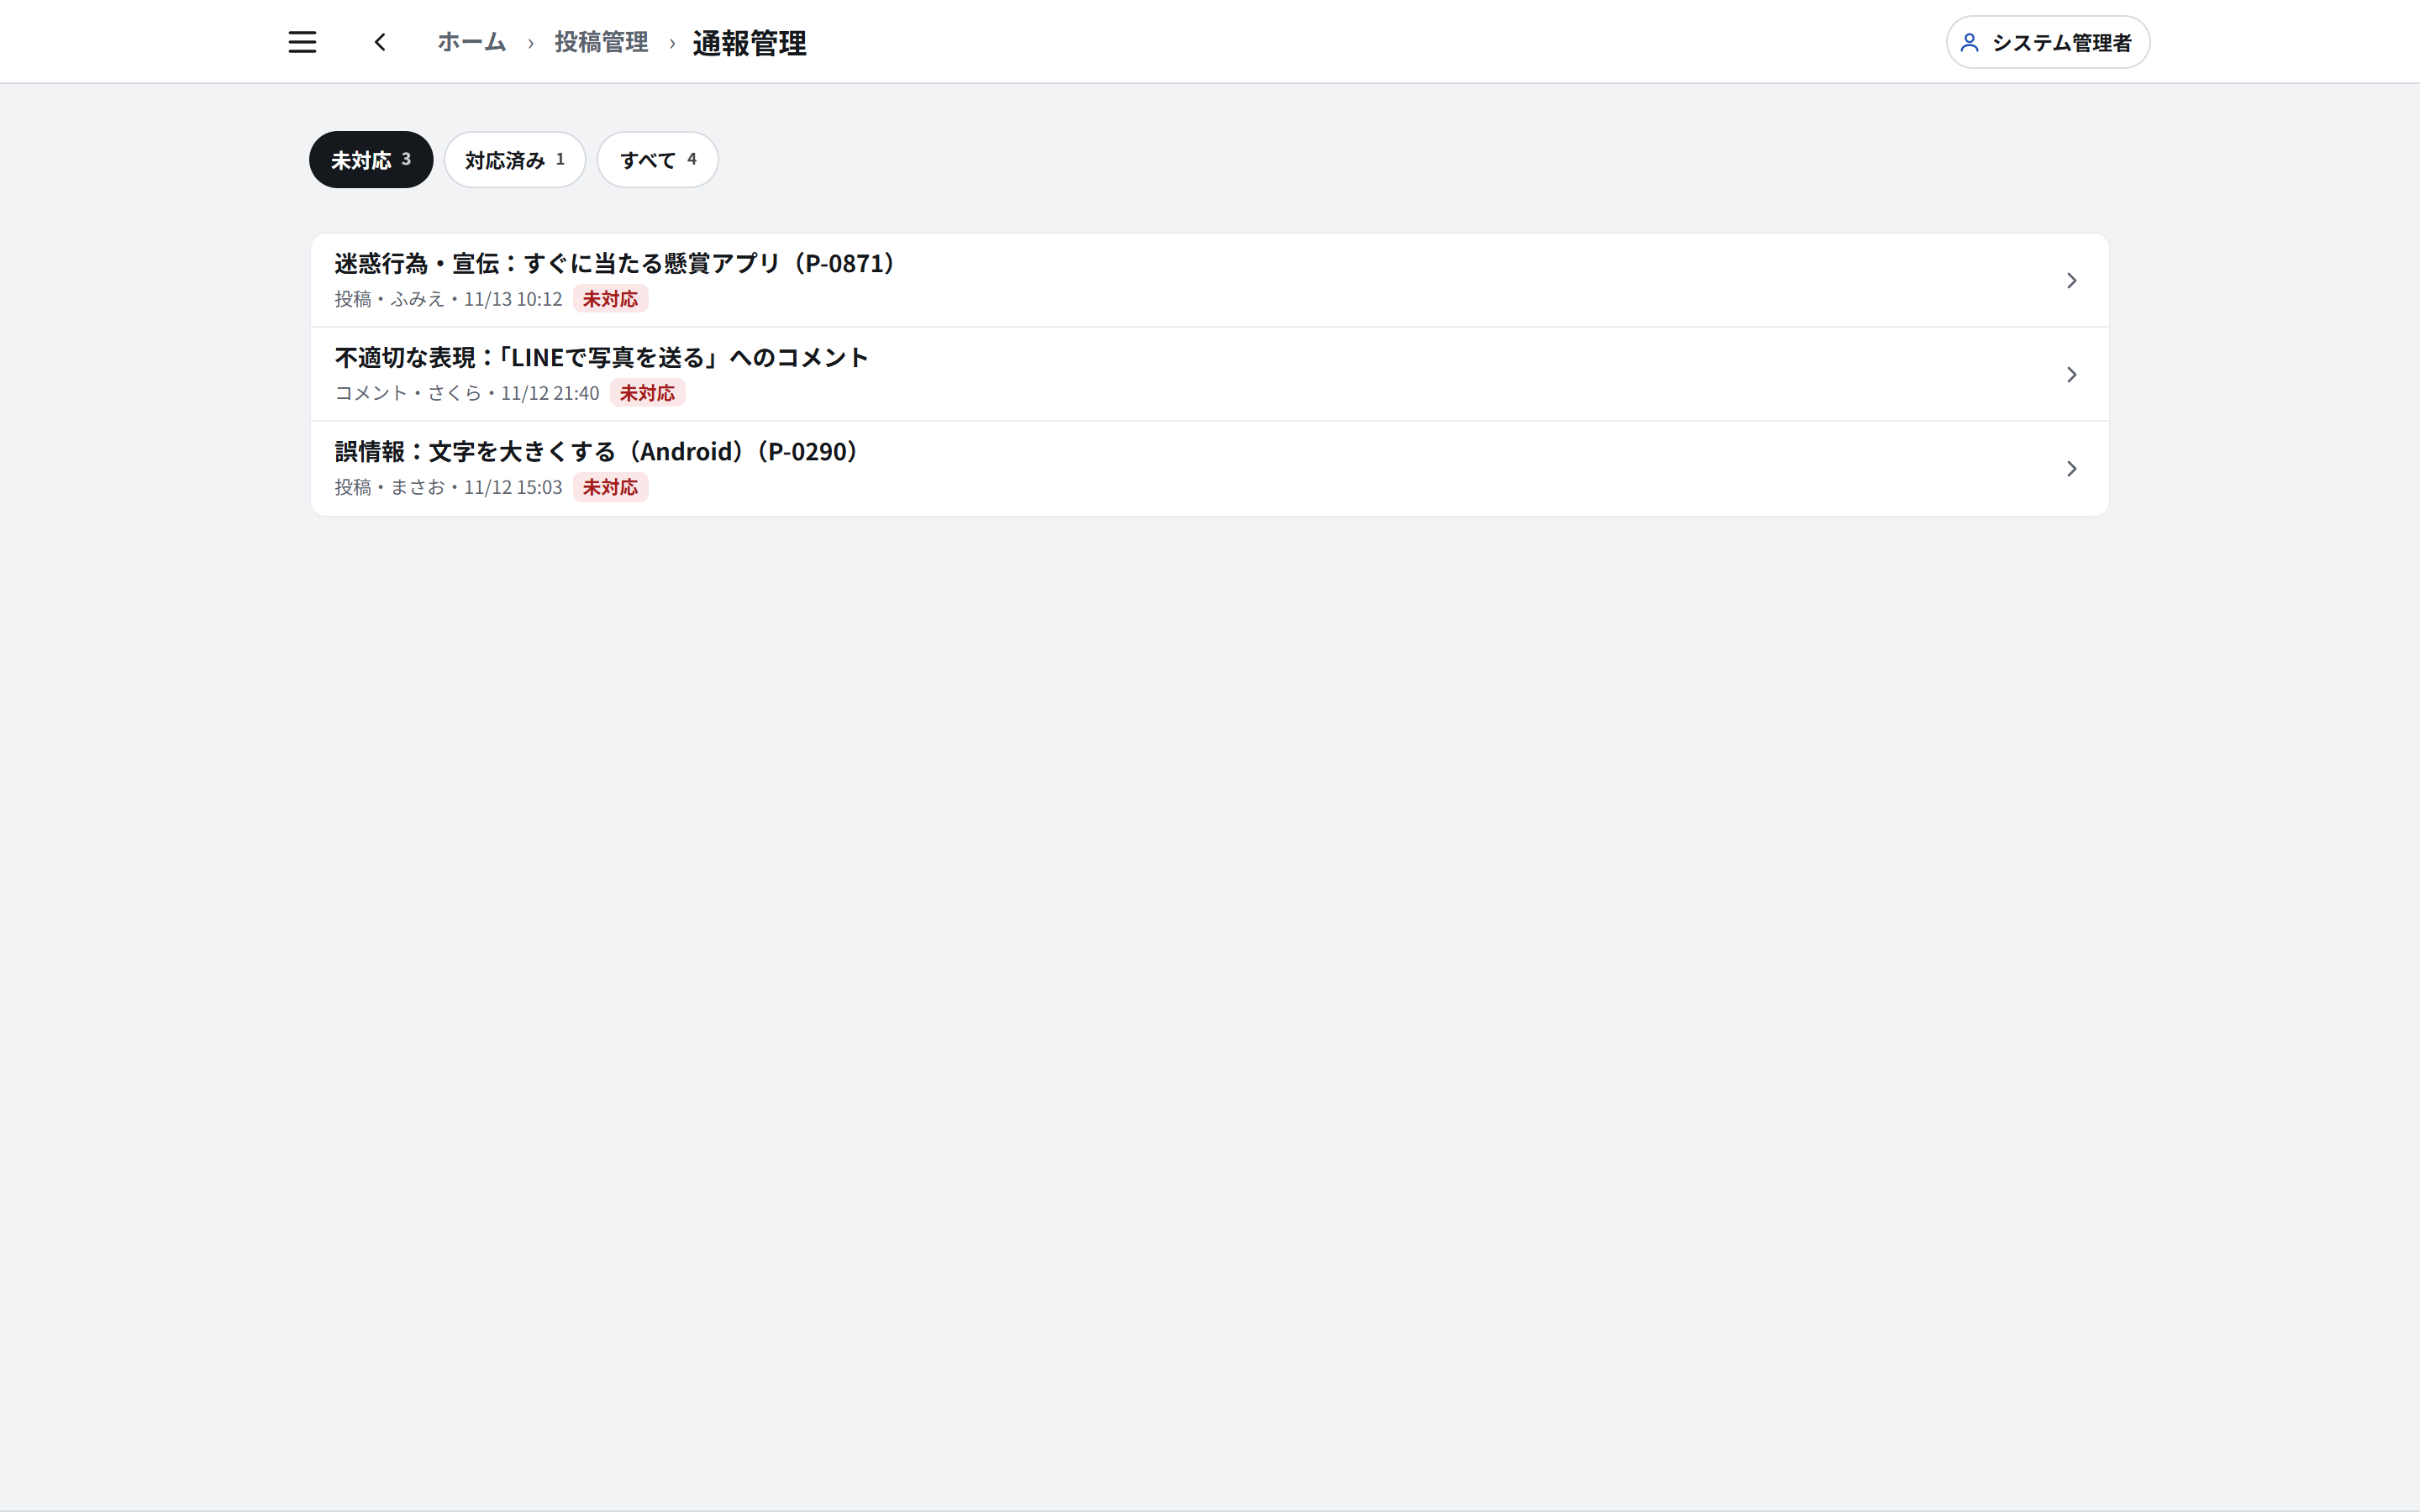
\includegraphics[width=\linewidth]{chapters/images/UI_Screen/admin/report.png}
  \caption{通報管理画面}
  \label{fig:ad_report}
\end{figure}


\subsubsection{通報詳細画面}

通報詳細画面を図\ref{fig:ad_report_details}に示す。

\begin{figure}[H]
  \centering

  \begin{subfigure}[t]{0.48\linewidth}
    \centering
    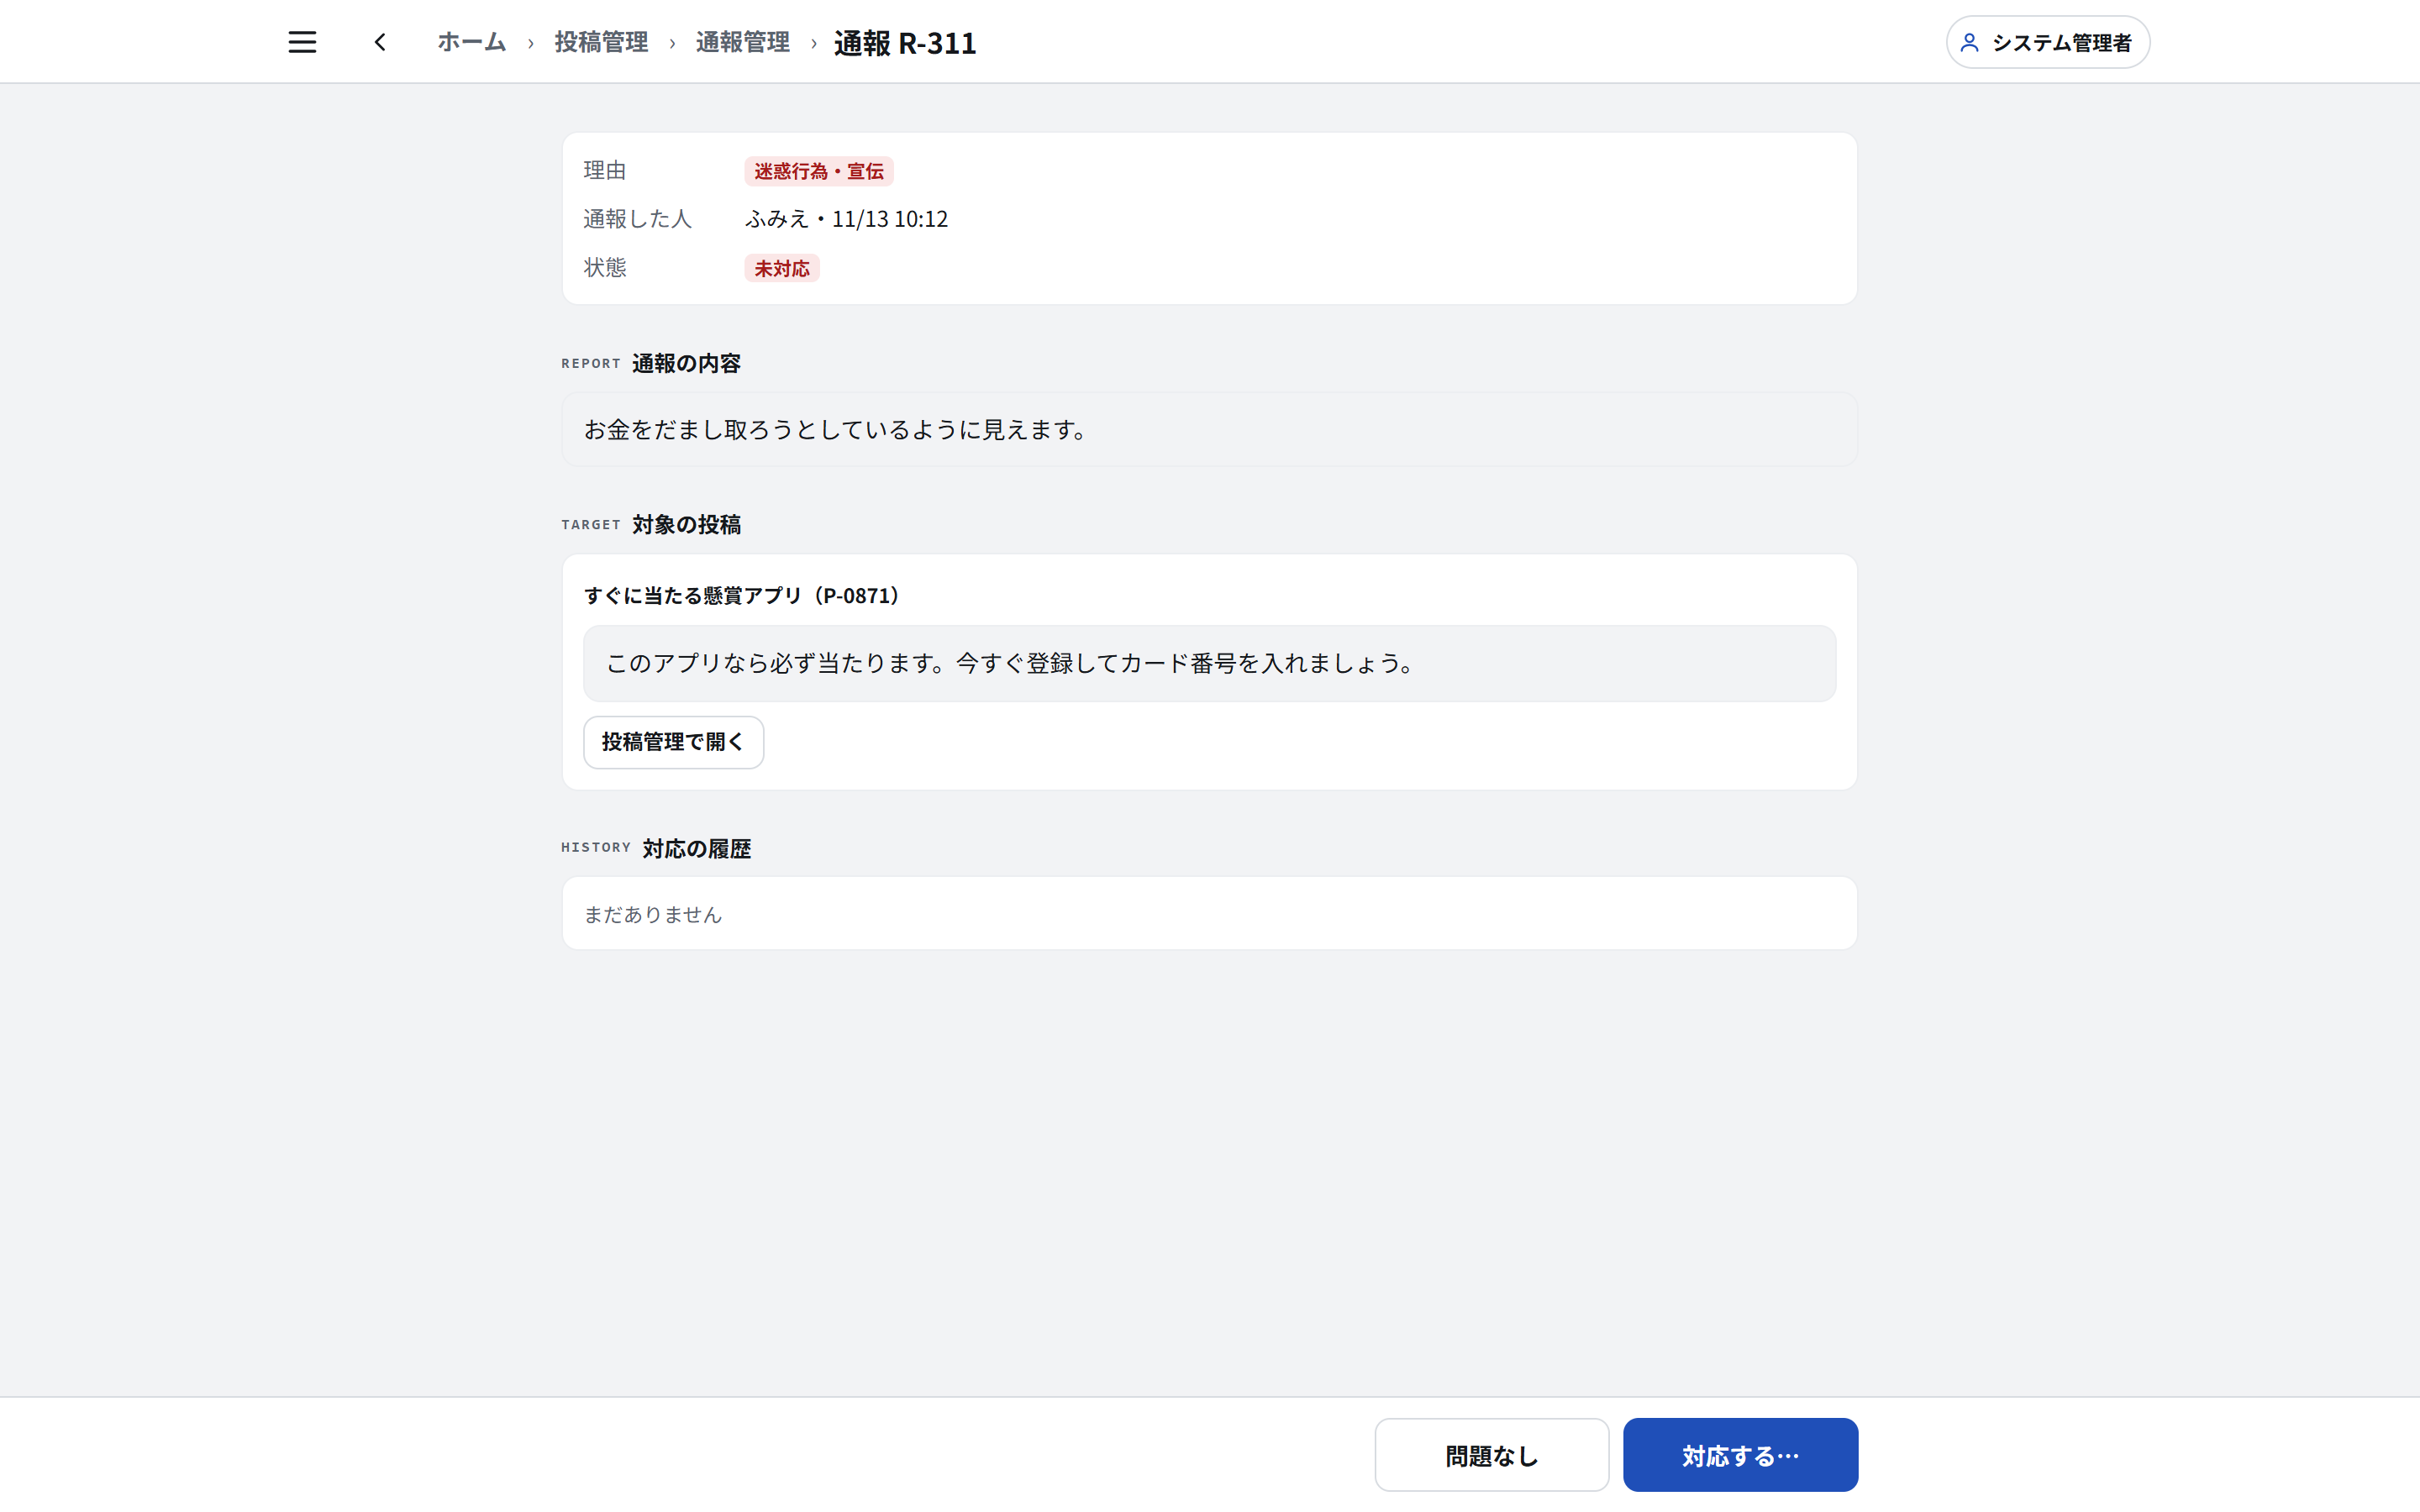
\includegraphics[width=\linewidth]{chapters/images/UI_Screen/admin/report_detail.png}
    \caption{通報詳細画面}
    \label{fig:ad_report_detail}
  \end{subfigure}
  \hfill
  \begin{subfigure}[t]{0.48\linewidth}
    \centering
    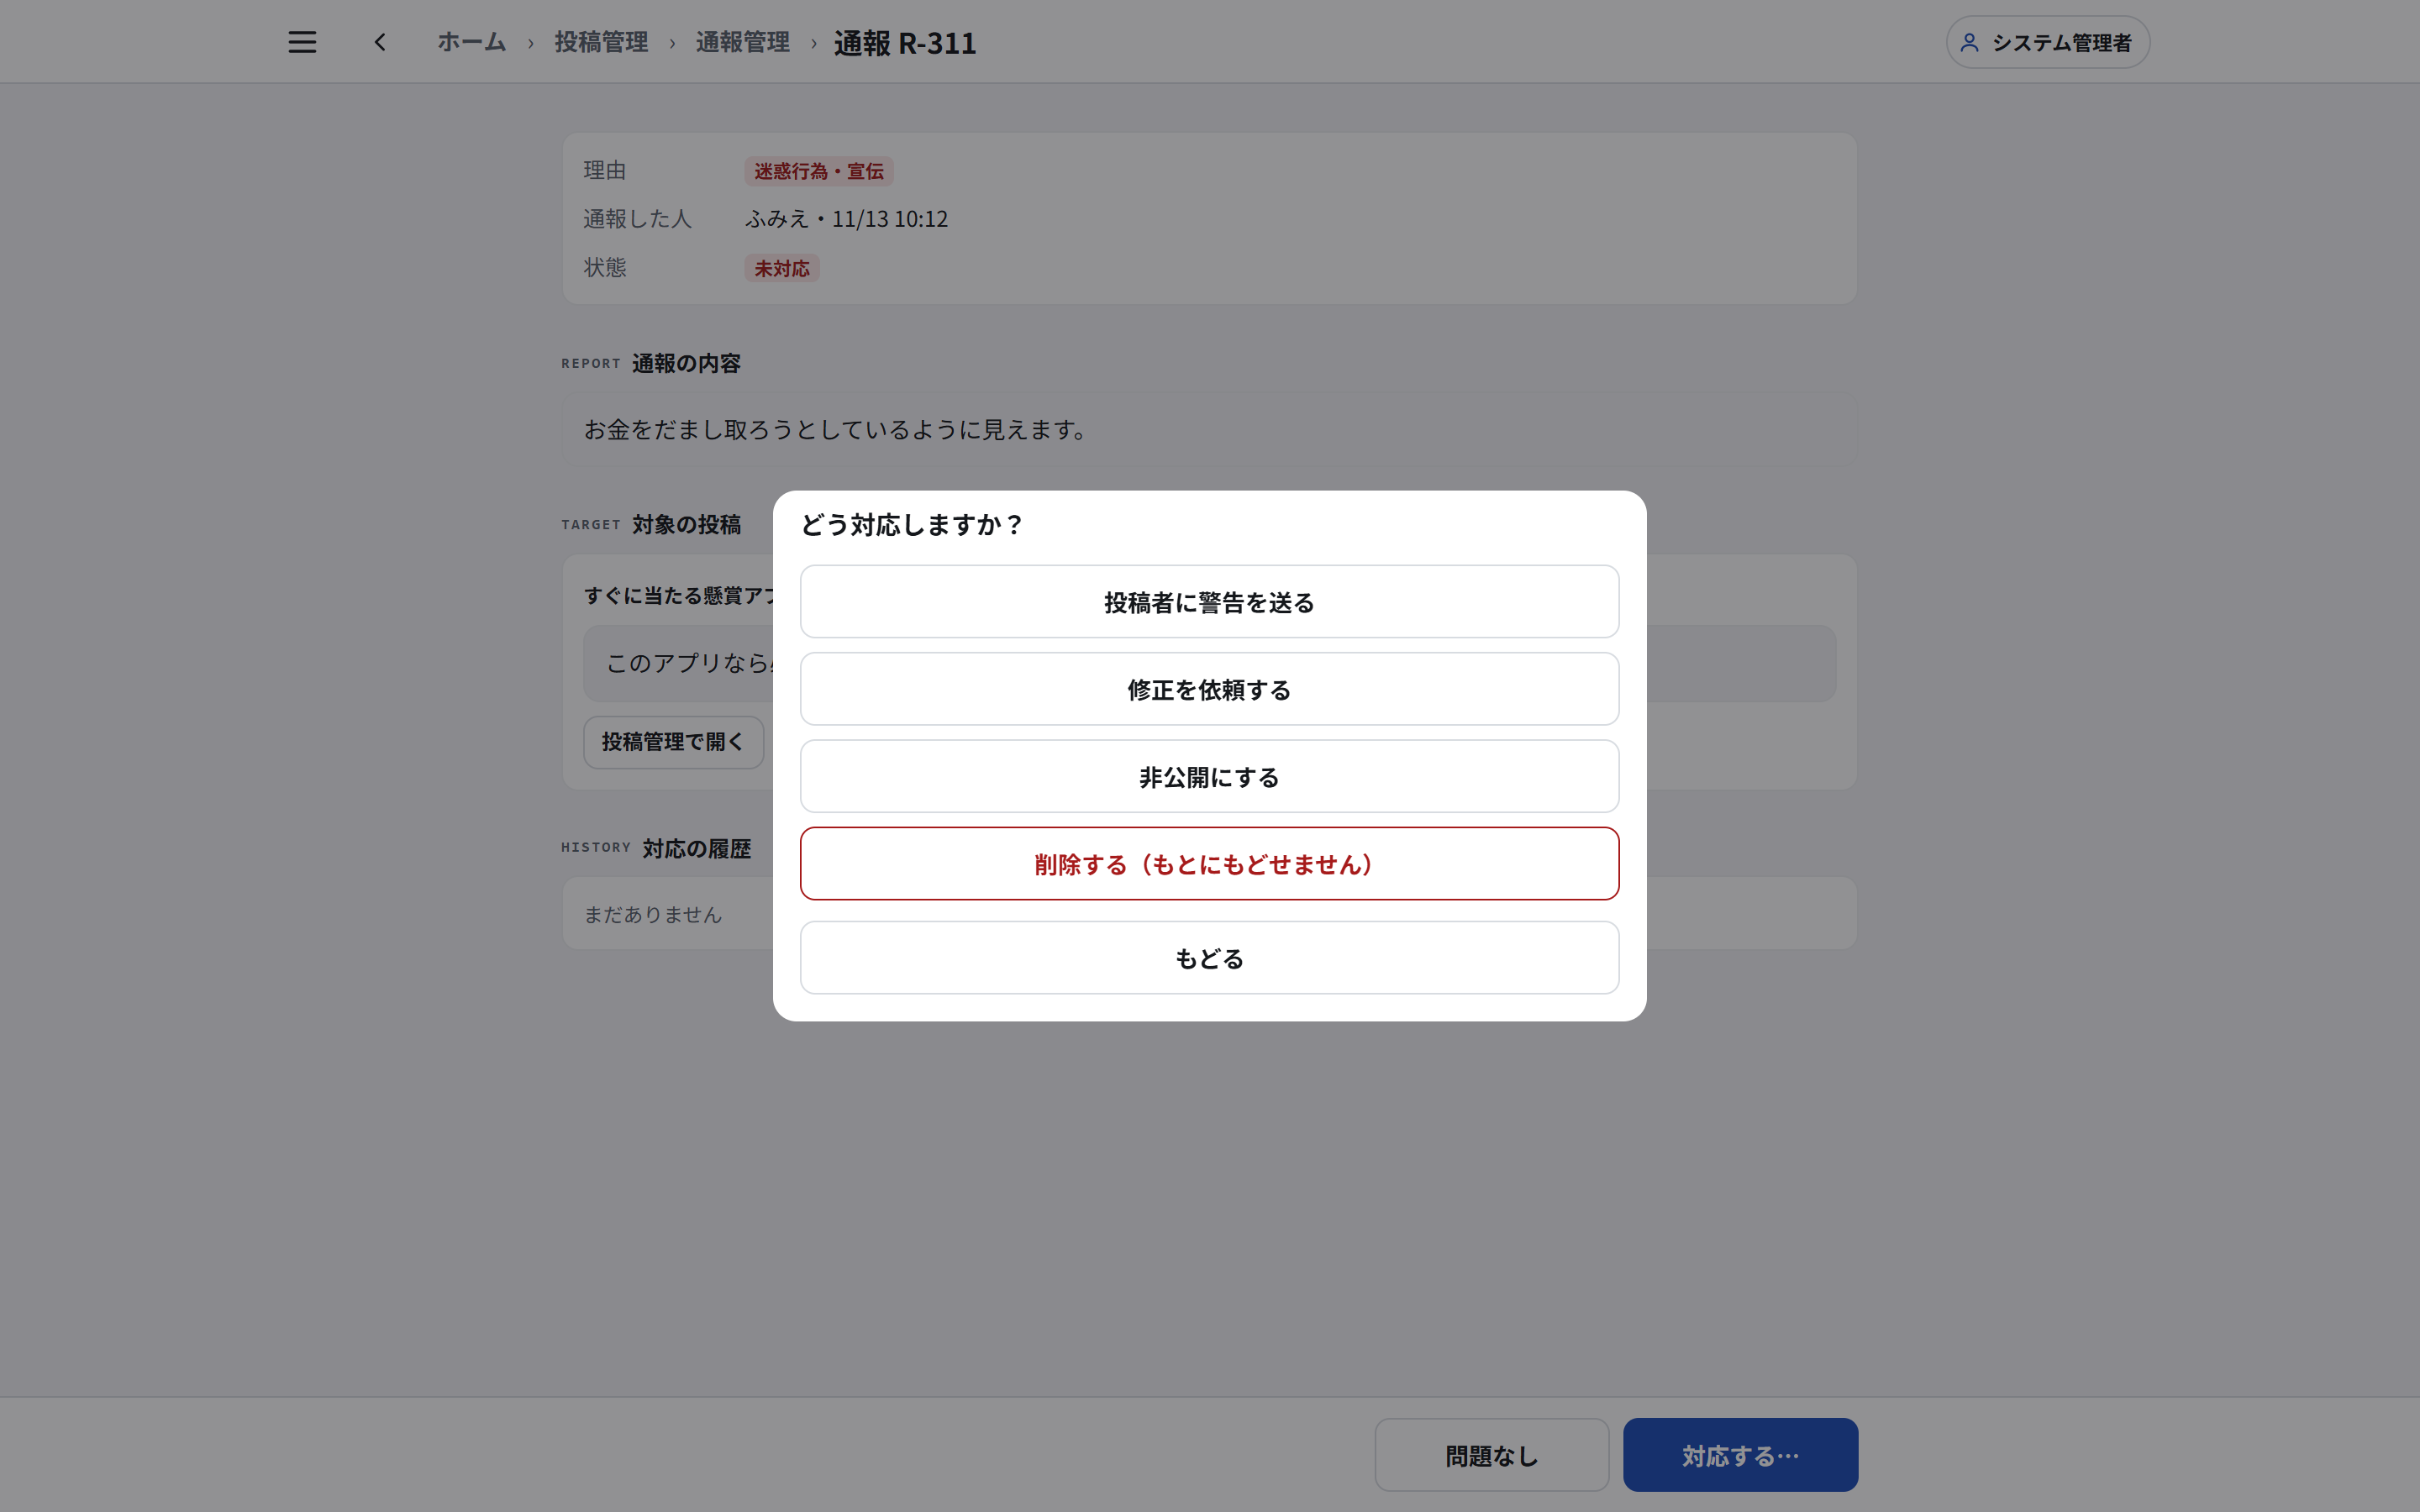
\includegraphics[width=\linewidth]{chapters/images/UI_Screen/admin/report_action.png}
    \caption{通報への対応画面}
    \label{fig:ad_report_action}
  \end{subfigure}

  \caption{通報詳細画面}
  \label{fig:ad_report_details}
\end{figure}

図\ref{fig:ad_report_detail}は、通報1件の内容を確認する画面である。通報の理由・通報した人・状態、通報の内容、対象の投稿またはコメントの本文、これまでの対応履歴が表示される。「投稿管理で開く」をクリックすると、対象の投稿の投稿詳細画面へ遷移する。問題がなければ「問題なし」を、対応が必要であれば「対応する…」をクリックする。

図\ref{fig:ad_report_action}は、通報詳細画面で「対応する…」をクリックすると表示される画面である。「投稿者に警告を送る」「修正を依頼する」「非公開にする」「削除する」から対応を選択することができる。対応の結果は通報した人に届き、対象の投稿にも反映される。


% =================================
\subsection{詳細管理画面}
% =================================

\subsubsection{詳細管理（パネル一覧）画面}

図\ref{fig:ad_detail_panel}は、ホーム画面で「詳細管理」をクリックすると表示される画面である。「お知らせ・イベント管理」「広告・タイアップ」「バージョン管理」のパネルが配置され、登録件数や現在のバージョンが表示される。クリックするとそれぞれの画面へ遷移する。

\begin{figure}[H]
  \centering
  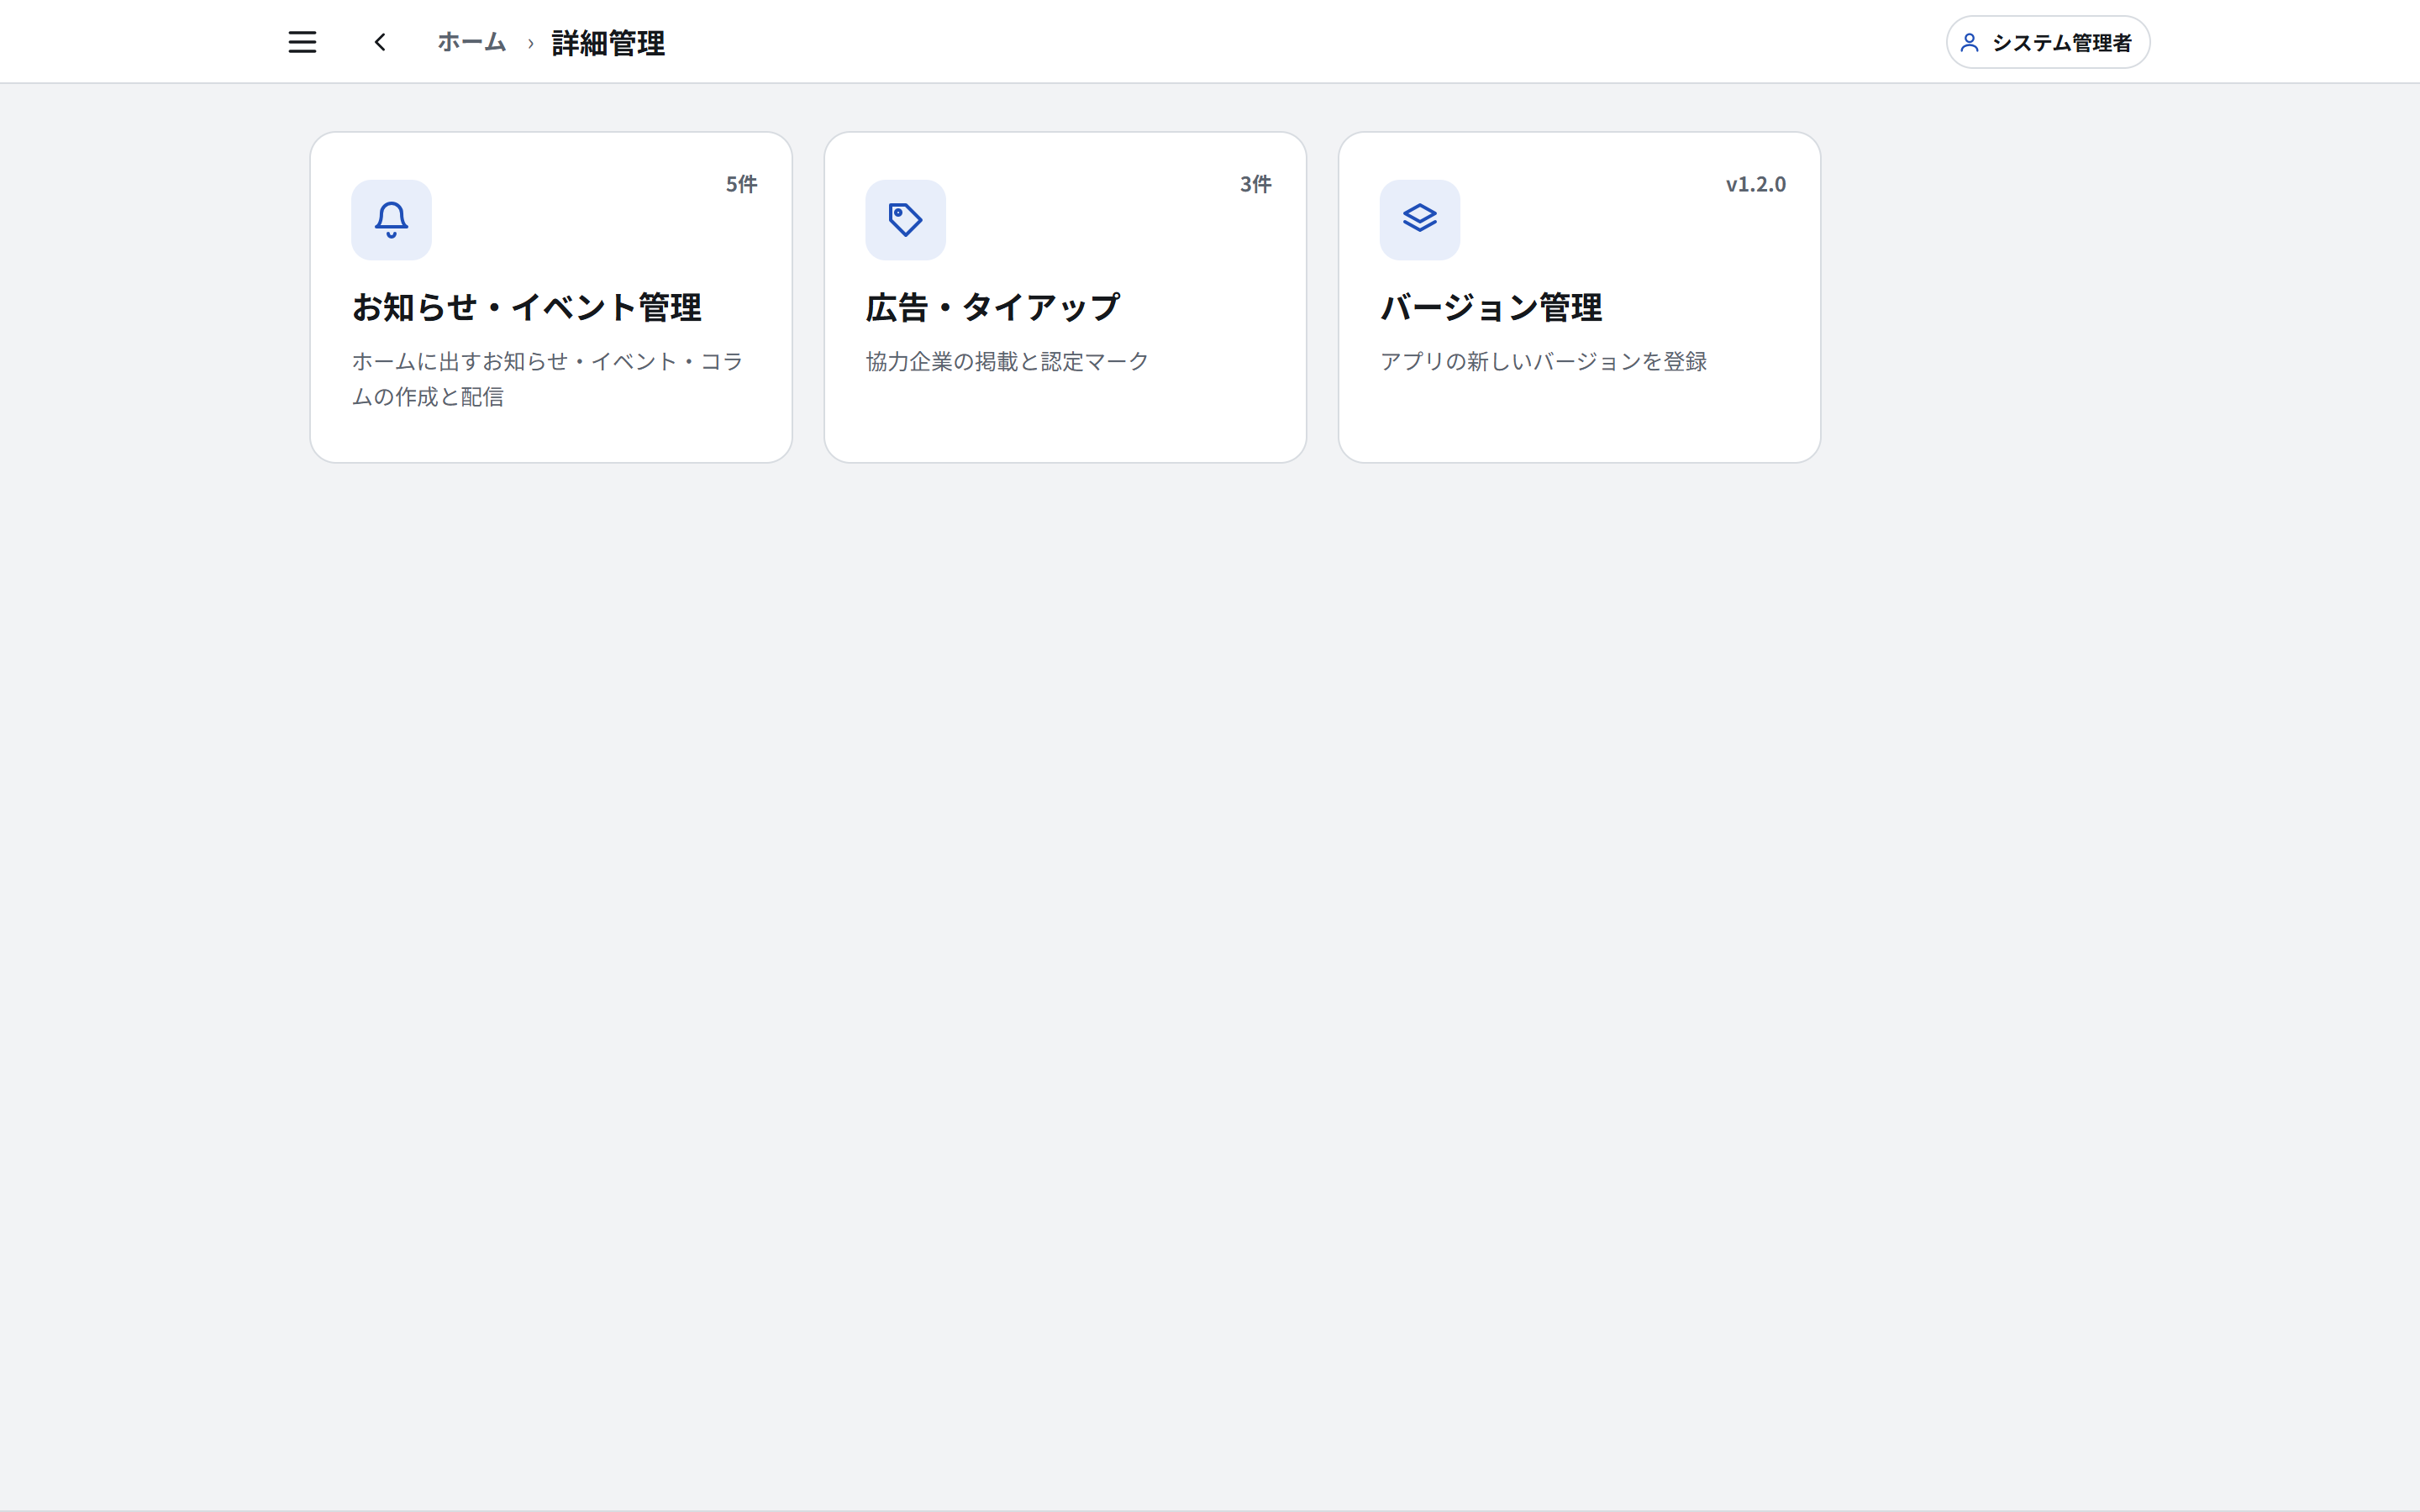
\includegraphics[width=\linewidth]{chapters/images/UI_Screen/admin/detail_panel.png}
  \caption{詳細管理（パネル一覧）画面}
  \label{fig:ad_detail_panel}
\end{figure}


\subsubsection{お知らせ・イベント管理画面}

お知らせ・イベント管理画面を図\ref{fig:ad_notices}に示す。

\begin{figure}[H]
  \centering

  \begin{subfigure}[t]{0.48\linewidth}
    \centering
    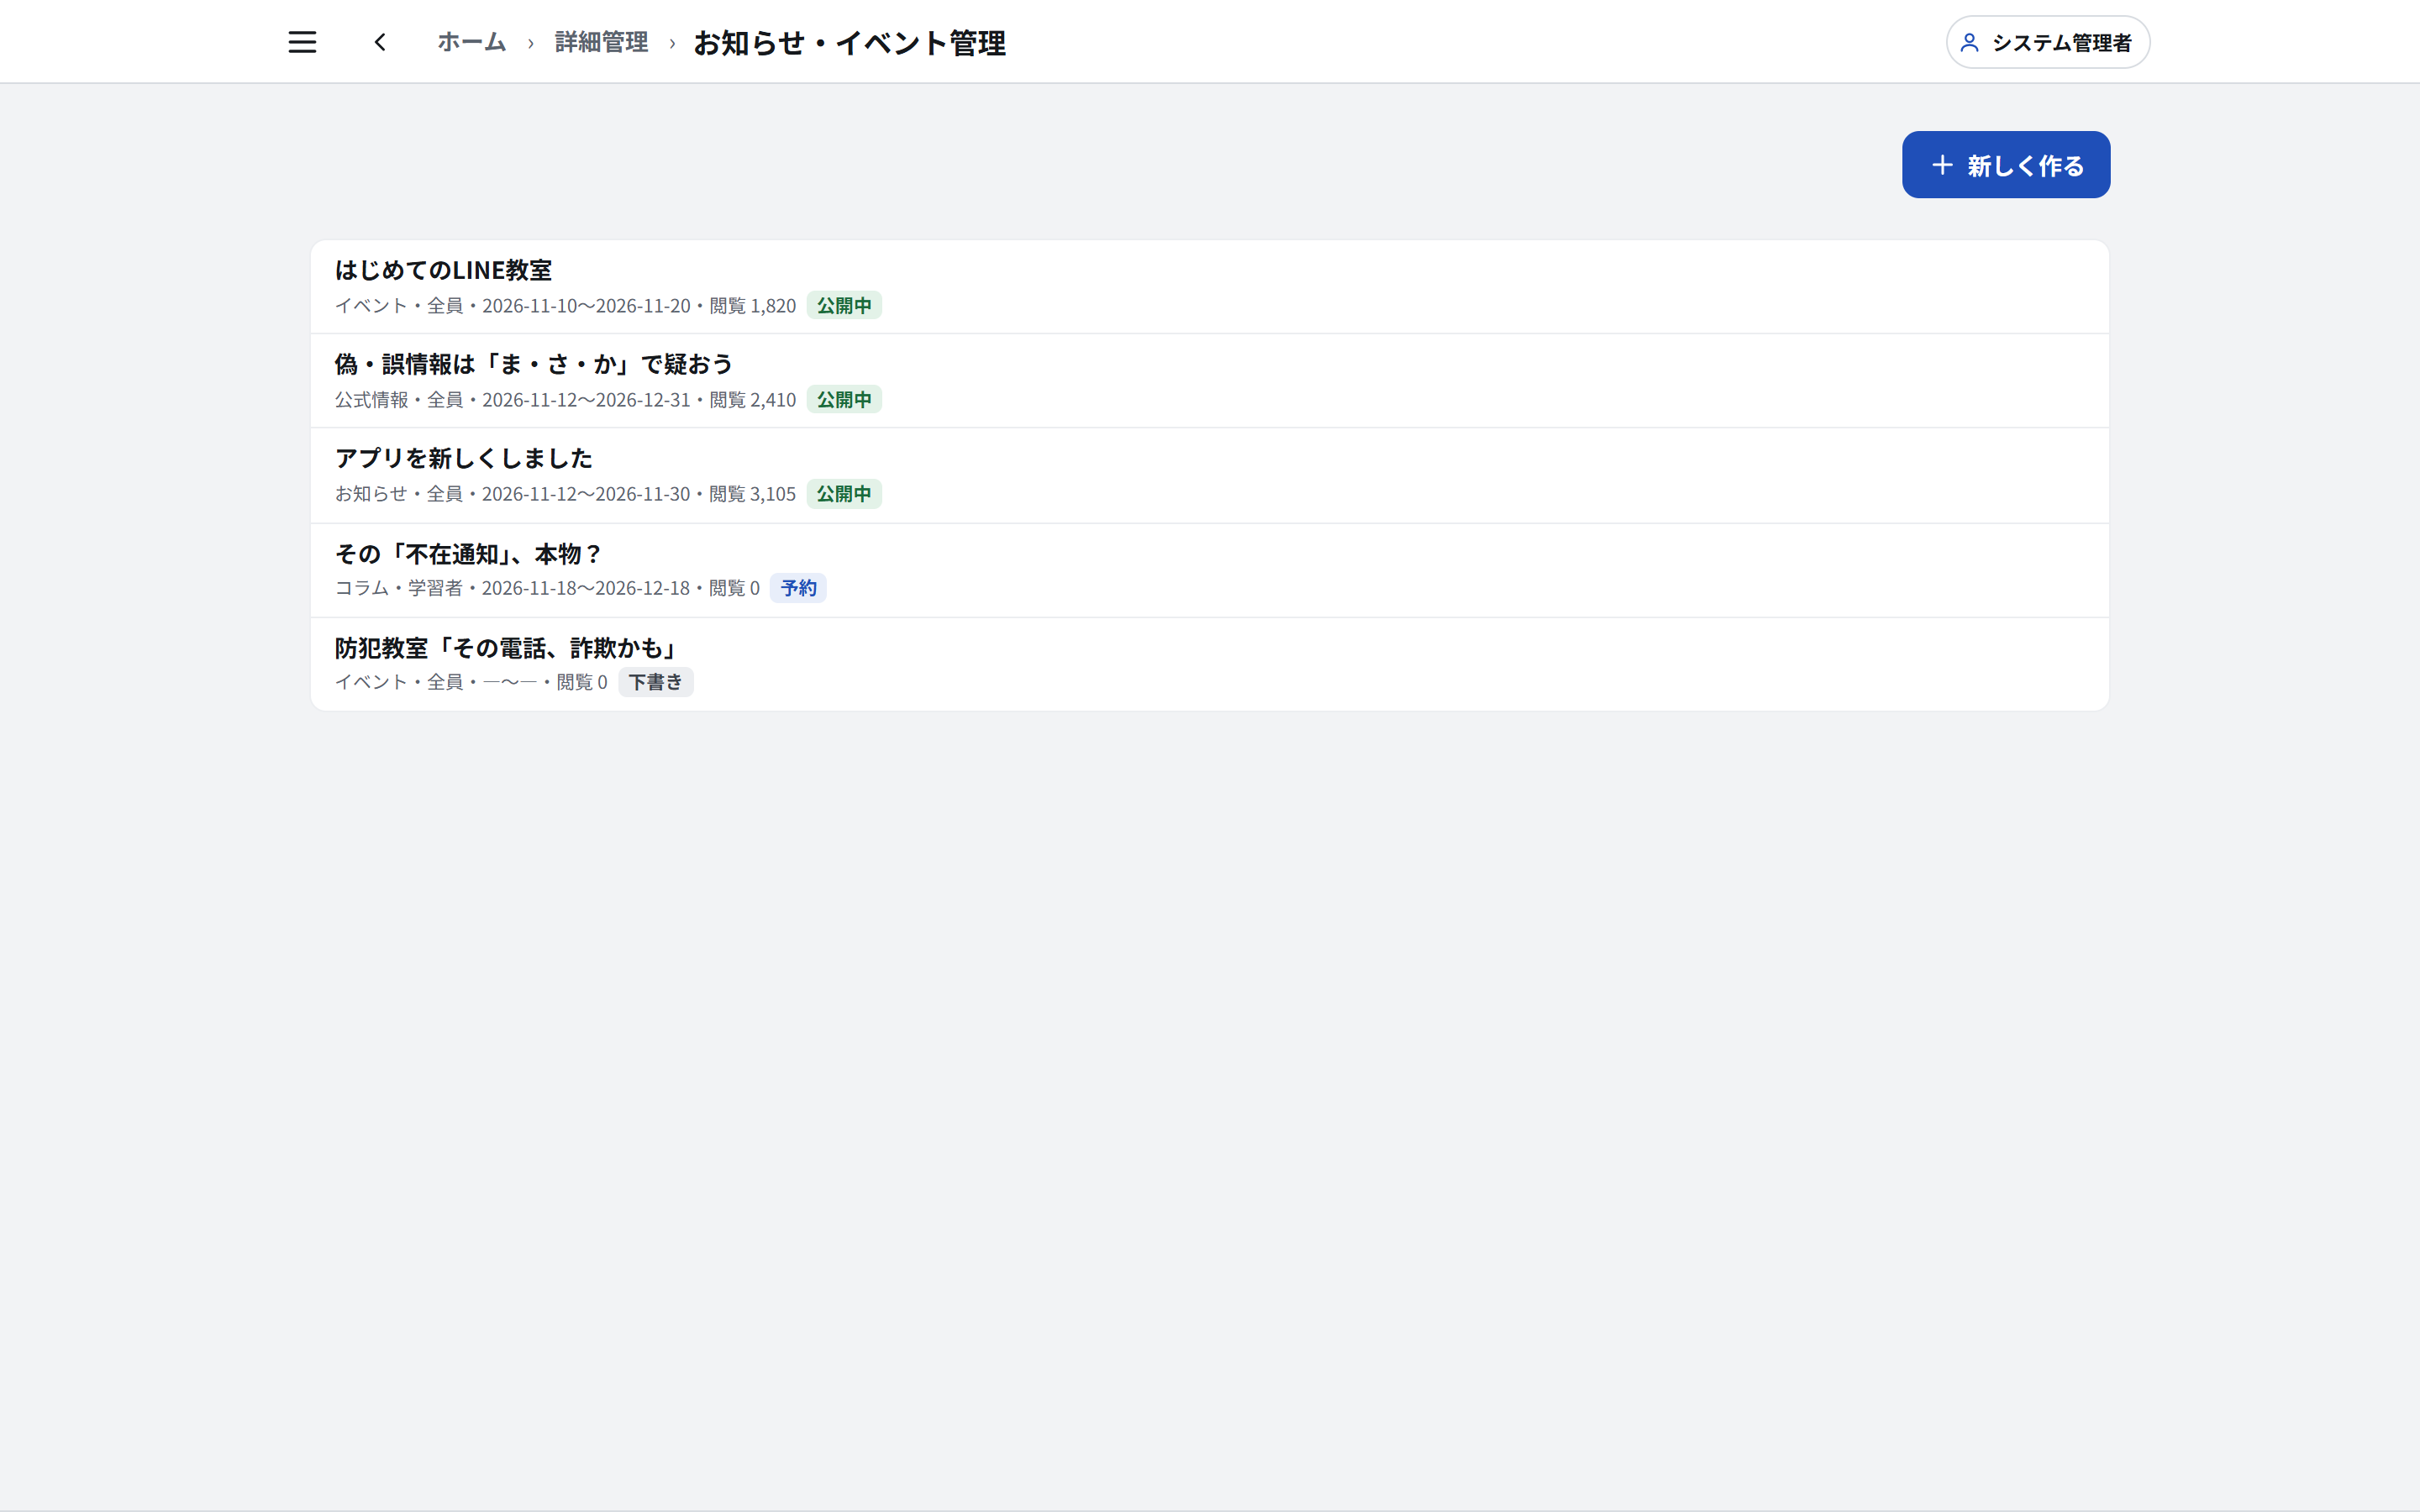
\includegraphics[width=\linewidth]{chapters/images/UI_Screen/admin/notice.png}
    \caption{お知らせ・イベント管理画面}
    \label{fig:ad_notice}
  \end{subfigure}
  \hfill
  \begin{subfigure}[t]{0.48\linewidth}
    \centering
    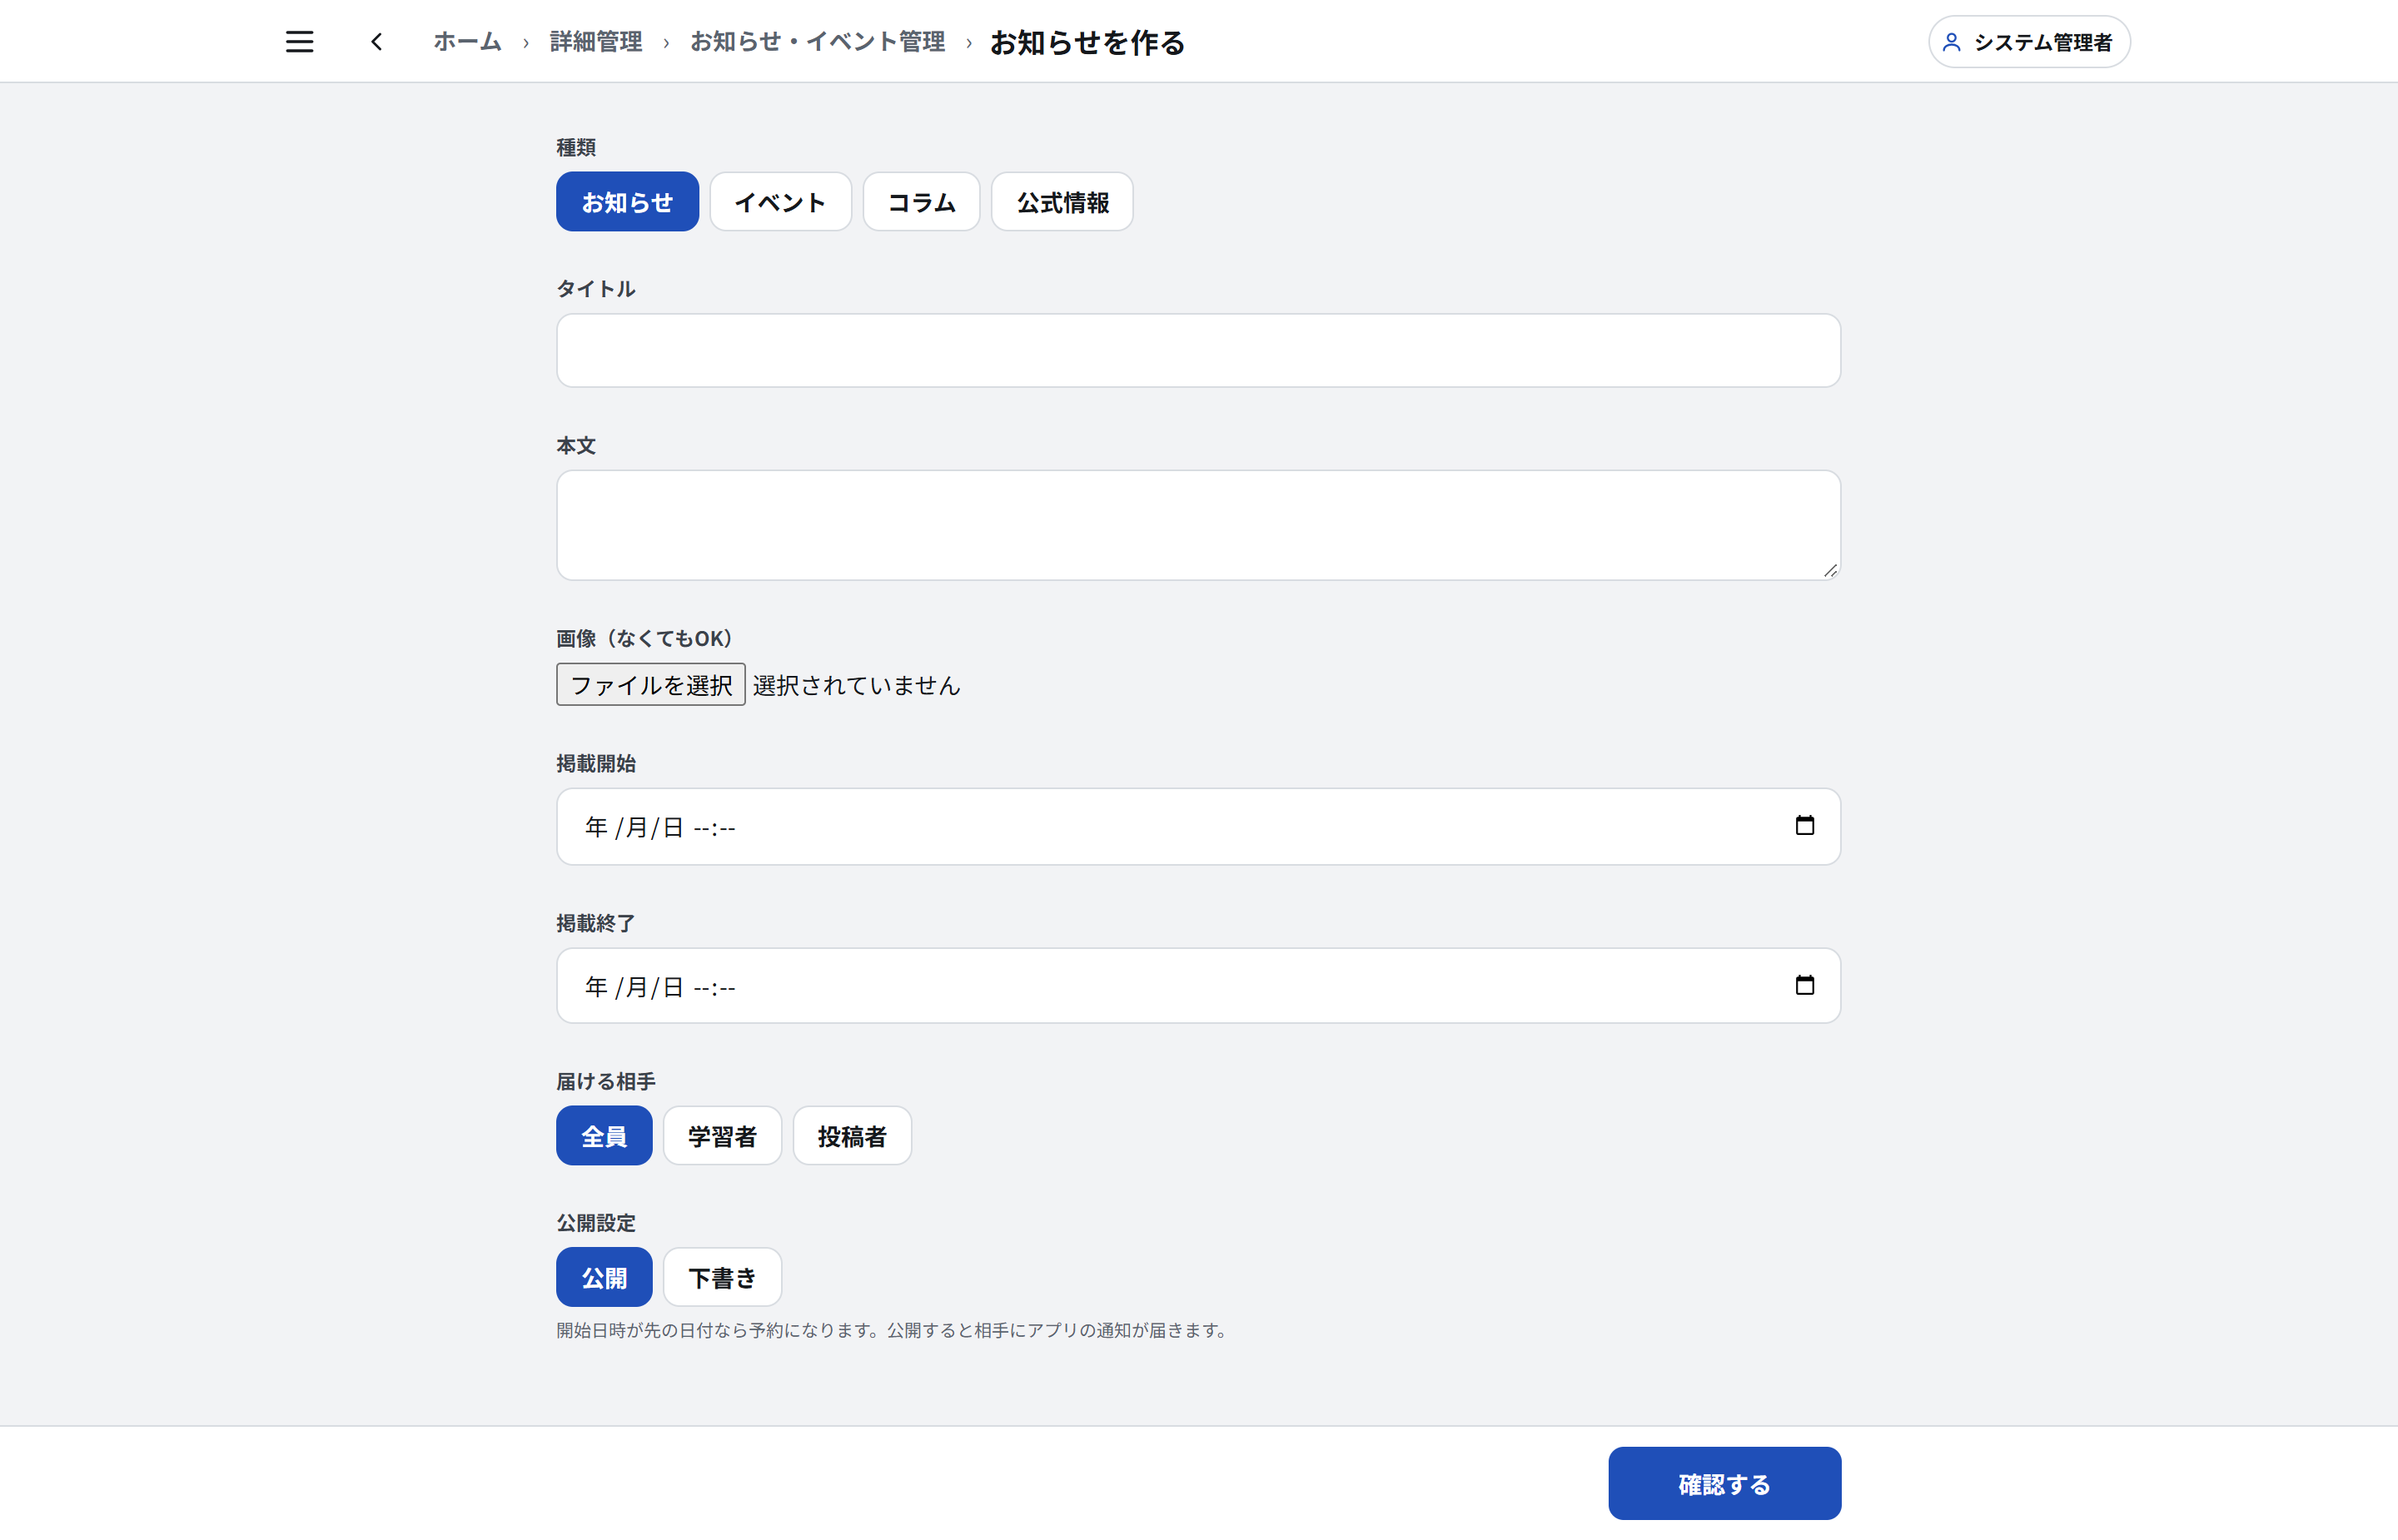
\includegraphics[width=\linewidth]{chapters/images/UI_Screen/admin/notice_new.png}
    \caption{お知らせ・イベント作成画面}
    \label{fig:ad_notice_new}
  \end{subfigure}

  \caption{お知らせ・イベント管理画面}
  \label{fig:ad_notices}
\end{figure}

図\ref{fig:ad_notice}は、アプリのホームに表示するお知らせ・イベント・コラム・公式情報の一覧を確認する画面である。一覧には種類・届ける相手・掲載期間・閲覧数・状態（公開中・予約・下書き）が表示される。「新しく作る」をクリックすると、お知らせ・イベント作成画面へ遷移する。

図\ref{fig:ad_notice_new}は、お知らせやイベントを新しく作成する画面である。種類（お知らせ・イベント・コラム・公式情報）、タイトル、本文、画像、掲載開始と掲載終了の日時、届ける相手（全員・学習者・投稿者）、公開設定（公開・下書き）を入力する。開始日時が先の日付の場合は予約となる。「確認する」をクリックして内容を確認したあとに配信すると、相手にアプリの通知が届く。


\subsubsection{広告・タイアップ画面}

広告・タイアップ画面を図\ref{fig:ad_ads}に示す。

\begin{figure}[H]
  \centering

  \begin{subfigure}[t]{0.48\linewidth}
    \centering
    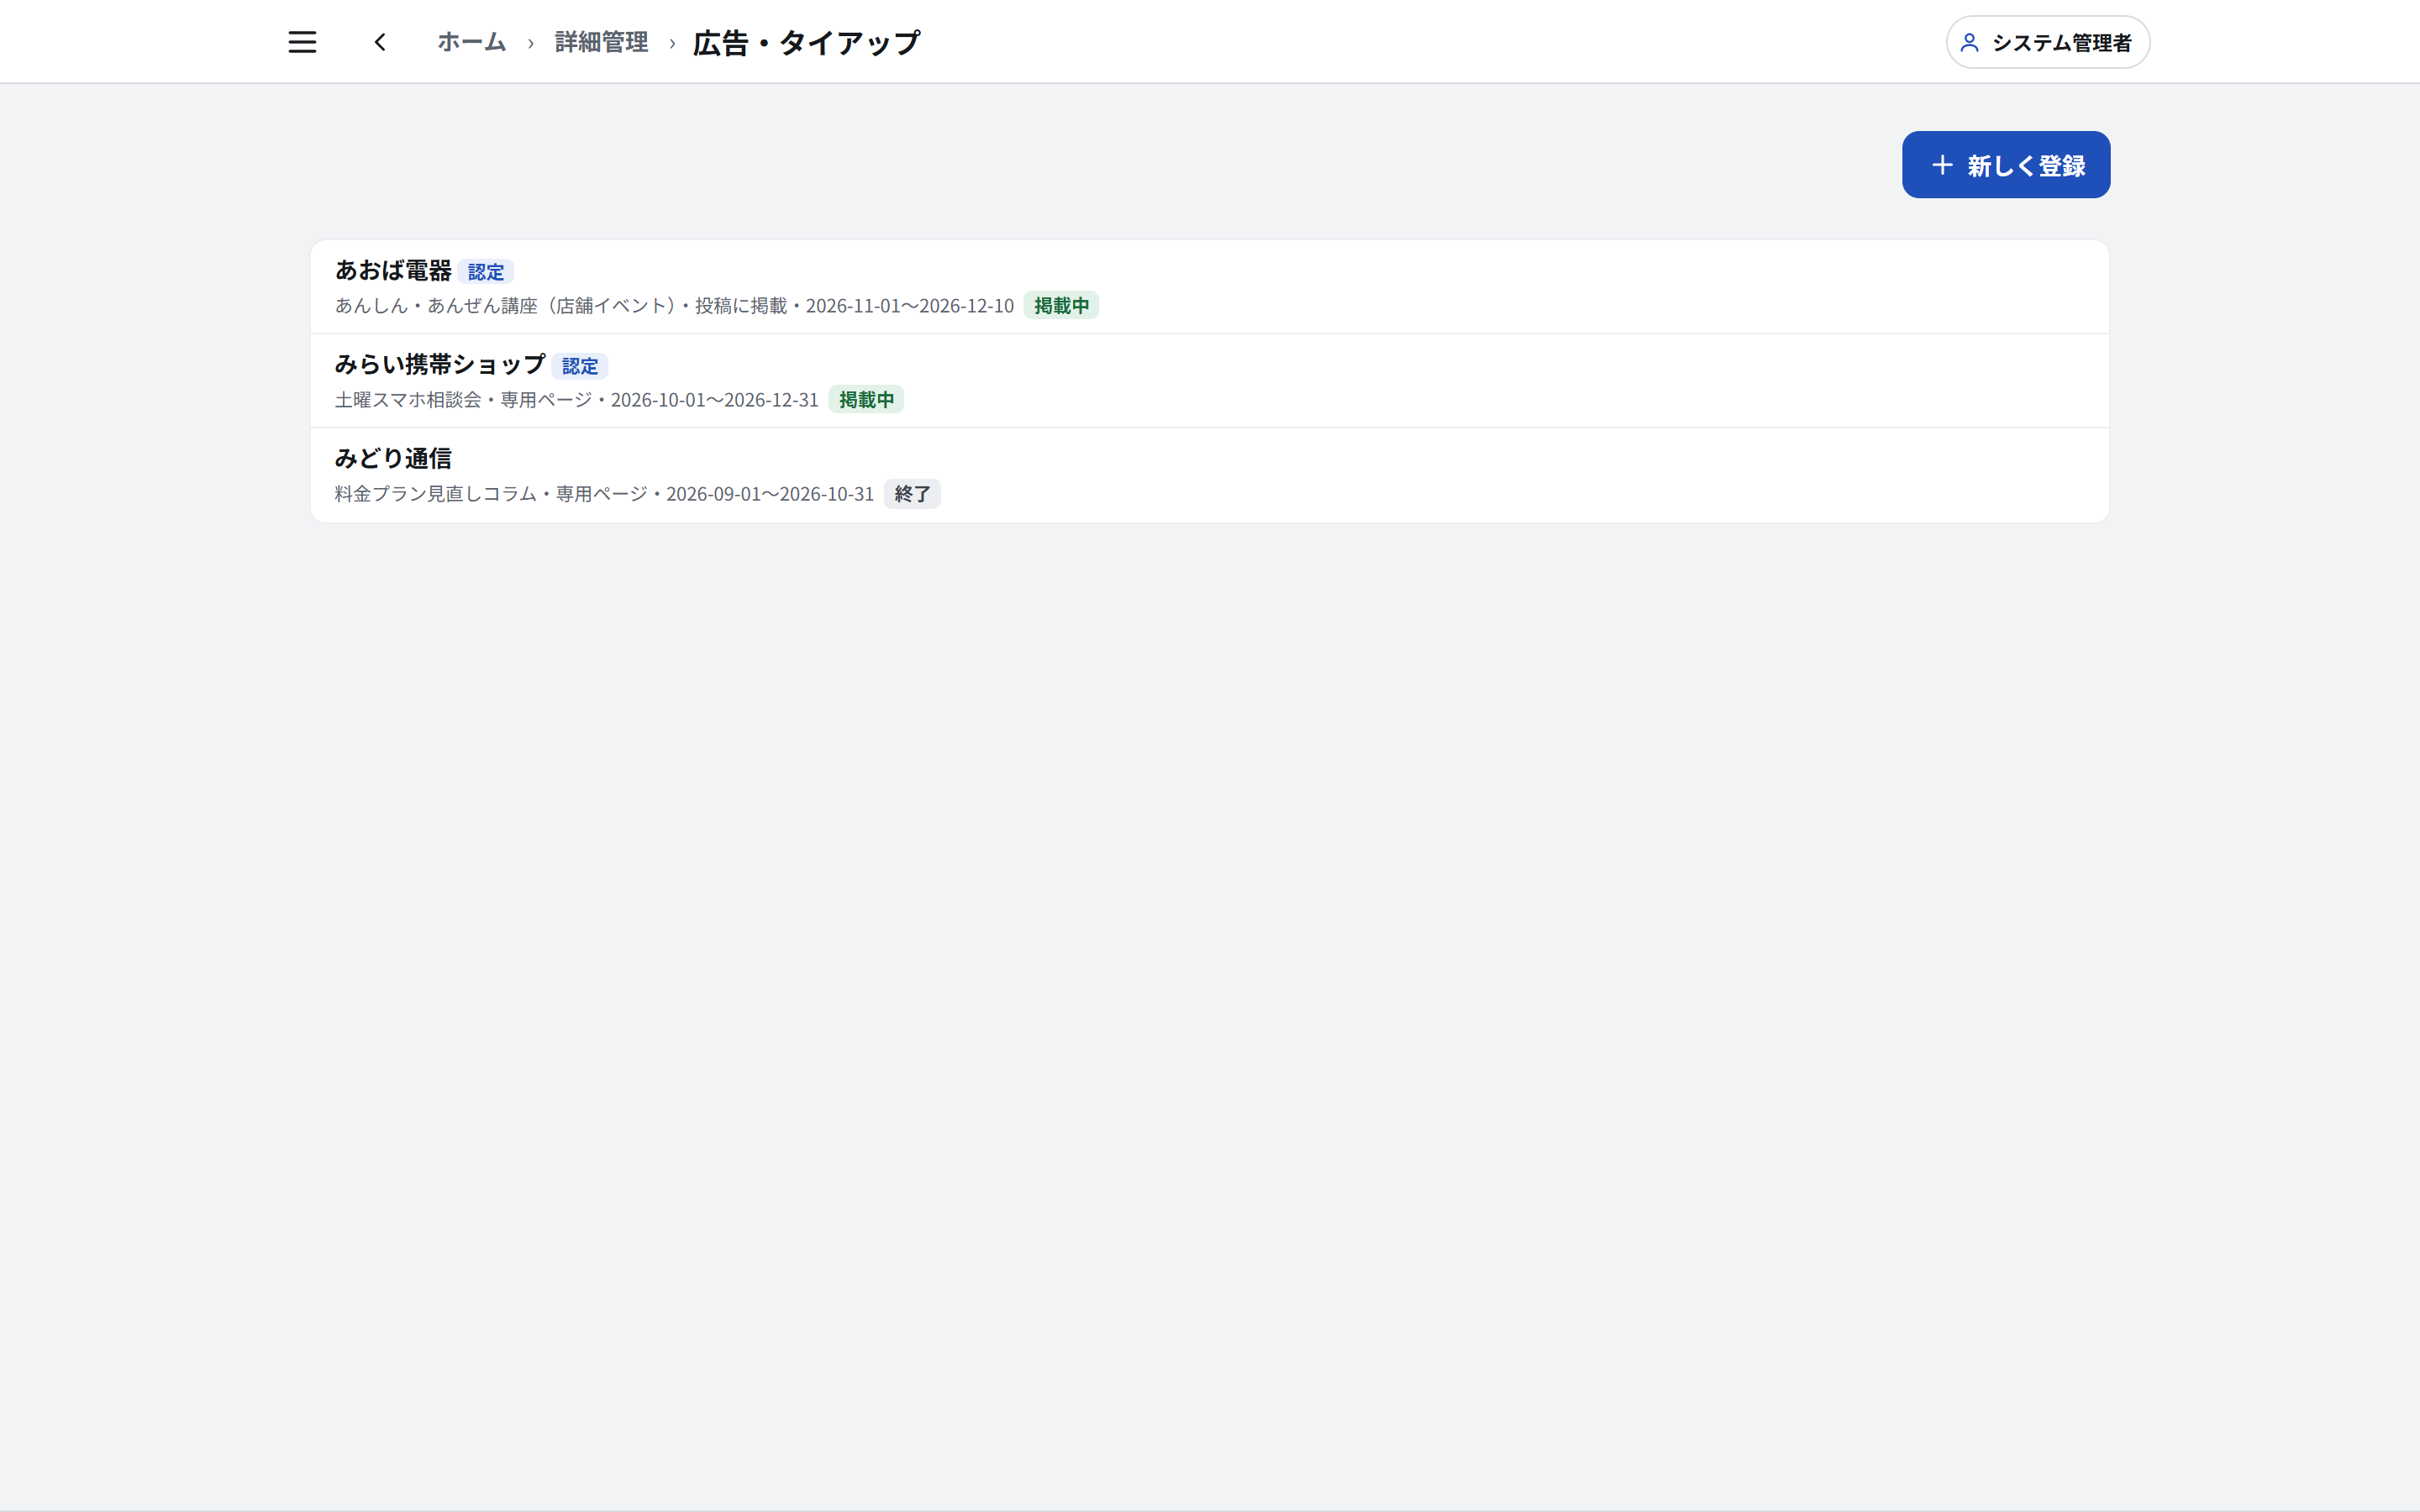
\includegraphics[width=\linewidth]{chapters/images/UI_Screen/admin/ad.png}
    \caption{広告・タイアップ画面}
    \label{fig:ad_ad}
  \end{subfigure}
  \hfill
  \begin{subfigure}[t]{0.48\linewidth}
    \centering
    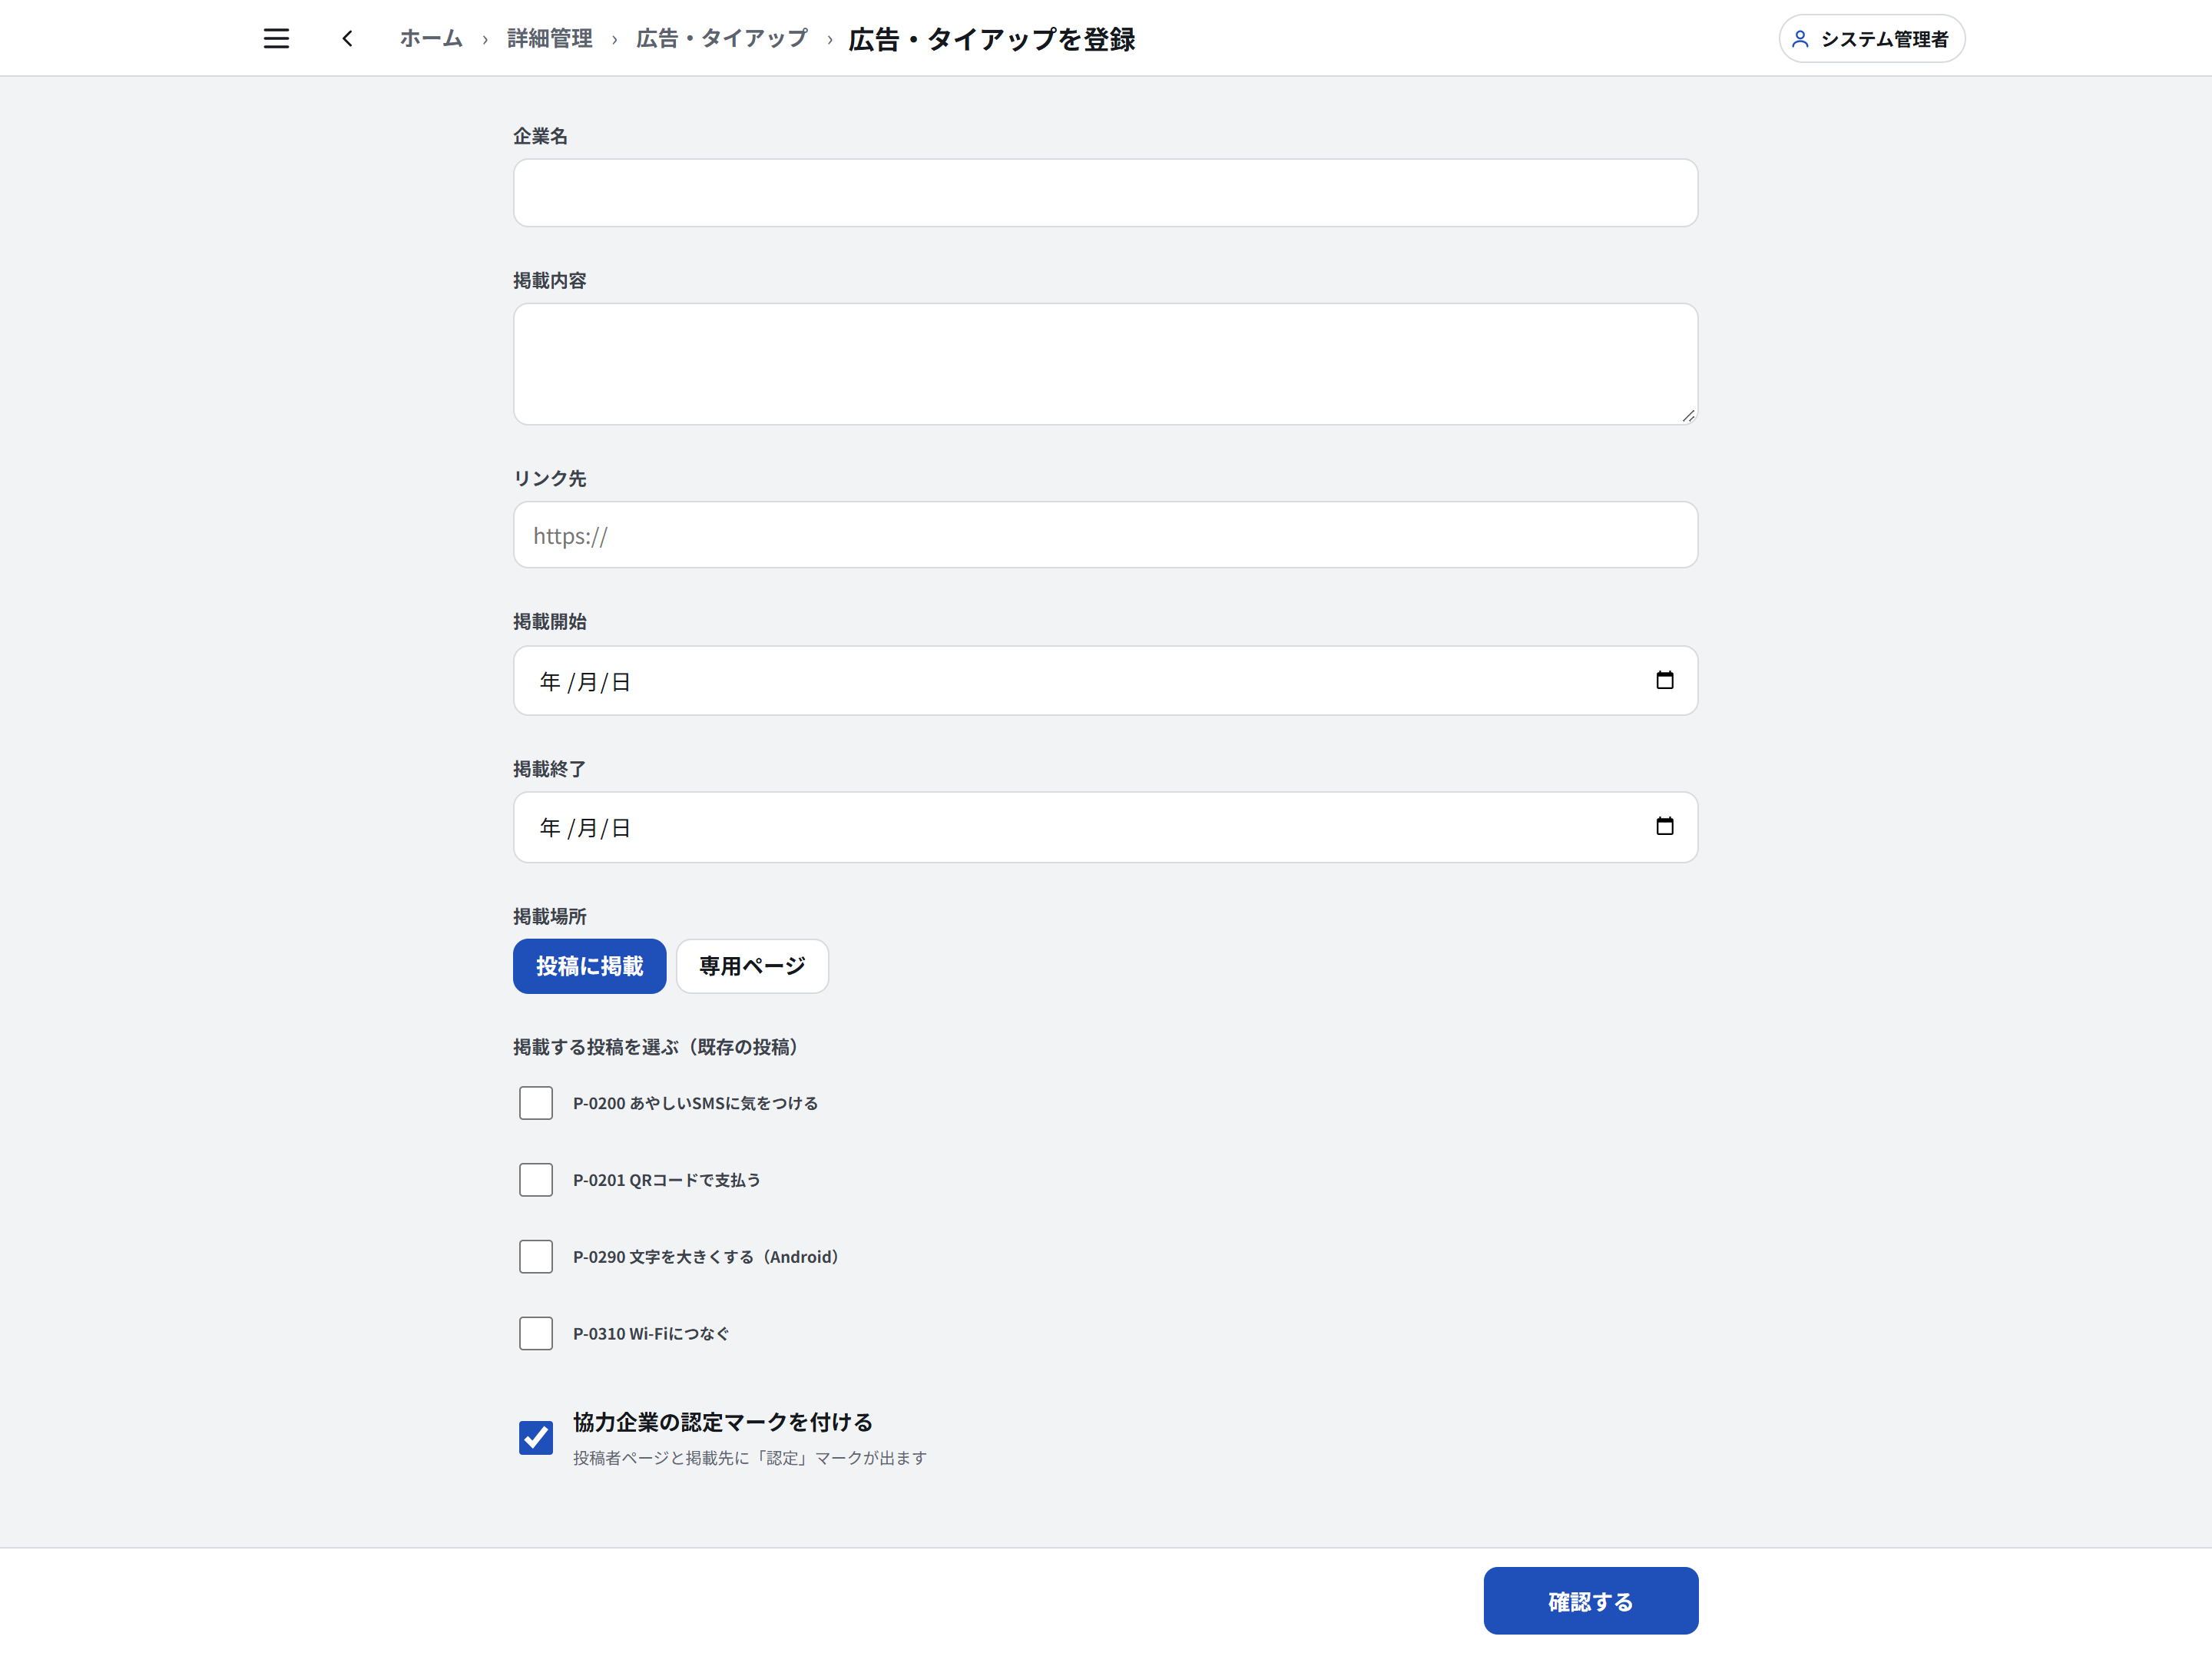
\includegraphics[width=\linewidth]{chapters/images/UI_Screen/admin/ad_new.png}
    \caption{広告・タイアップ登録画面}
    \label{fig:ad_ad_new}
  \end{subfigure}

  \caption{広告・タイアップ画面}
  \label{fig:ad_ads}
\end{figure}

図\ref{fig:ad_ad}は、協力企業の広告・タイアップの一覧を確認する画面である。一覧には企業名・認定マークの有無・掲載内容・掲載場所・掲載期間・状態が表示される。「新しく登録」をクリックすると、広告・タイアップ登録画面へ遷移する。

図\ref{fig:ad_ad_new}は、広告・タイアップを新しく登録する画面である。企業名・掲載内容・リンク先・掲載期間・掲載場所（投稿に掲載・専用ページ）を入力する。投稿に掲載する場合は、掲載する投稿を既存の投稿から選択する。認定マークを付けると、投稿者ページと掲載先に「認定」マークが表示される。「確認する」をクリックして内容を確認したあとに登録する。


\subsubsection{バージョン管理画面}

バージョン管理画面を図\ref{fig:ad_versions}に示す。

\begin{figure}[H]
  \centering

  \begin{subfigure}[t]{0.48\linewidth}
    \centering
    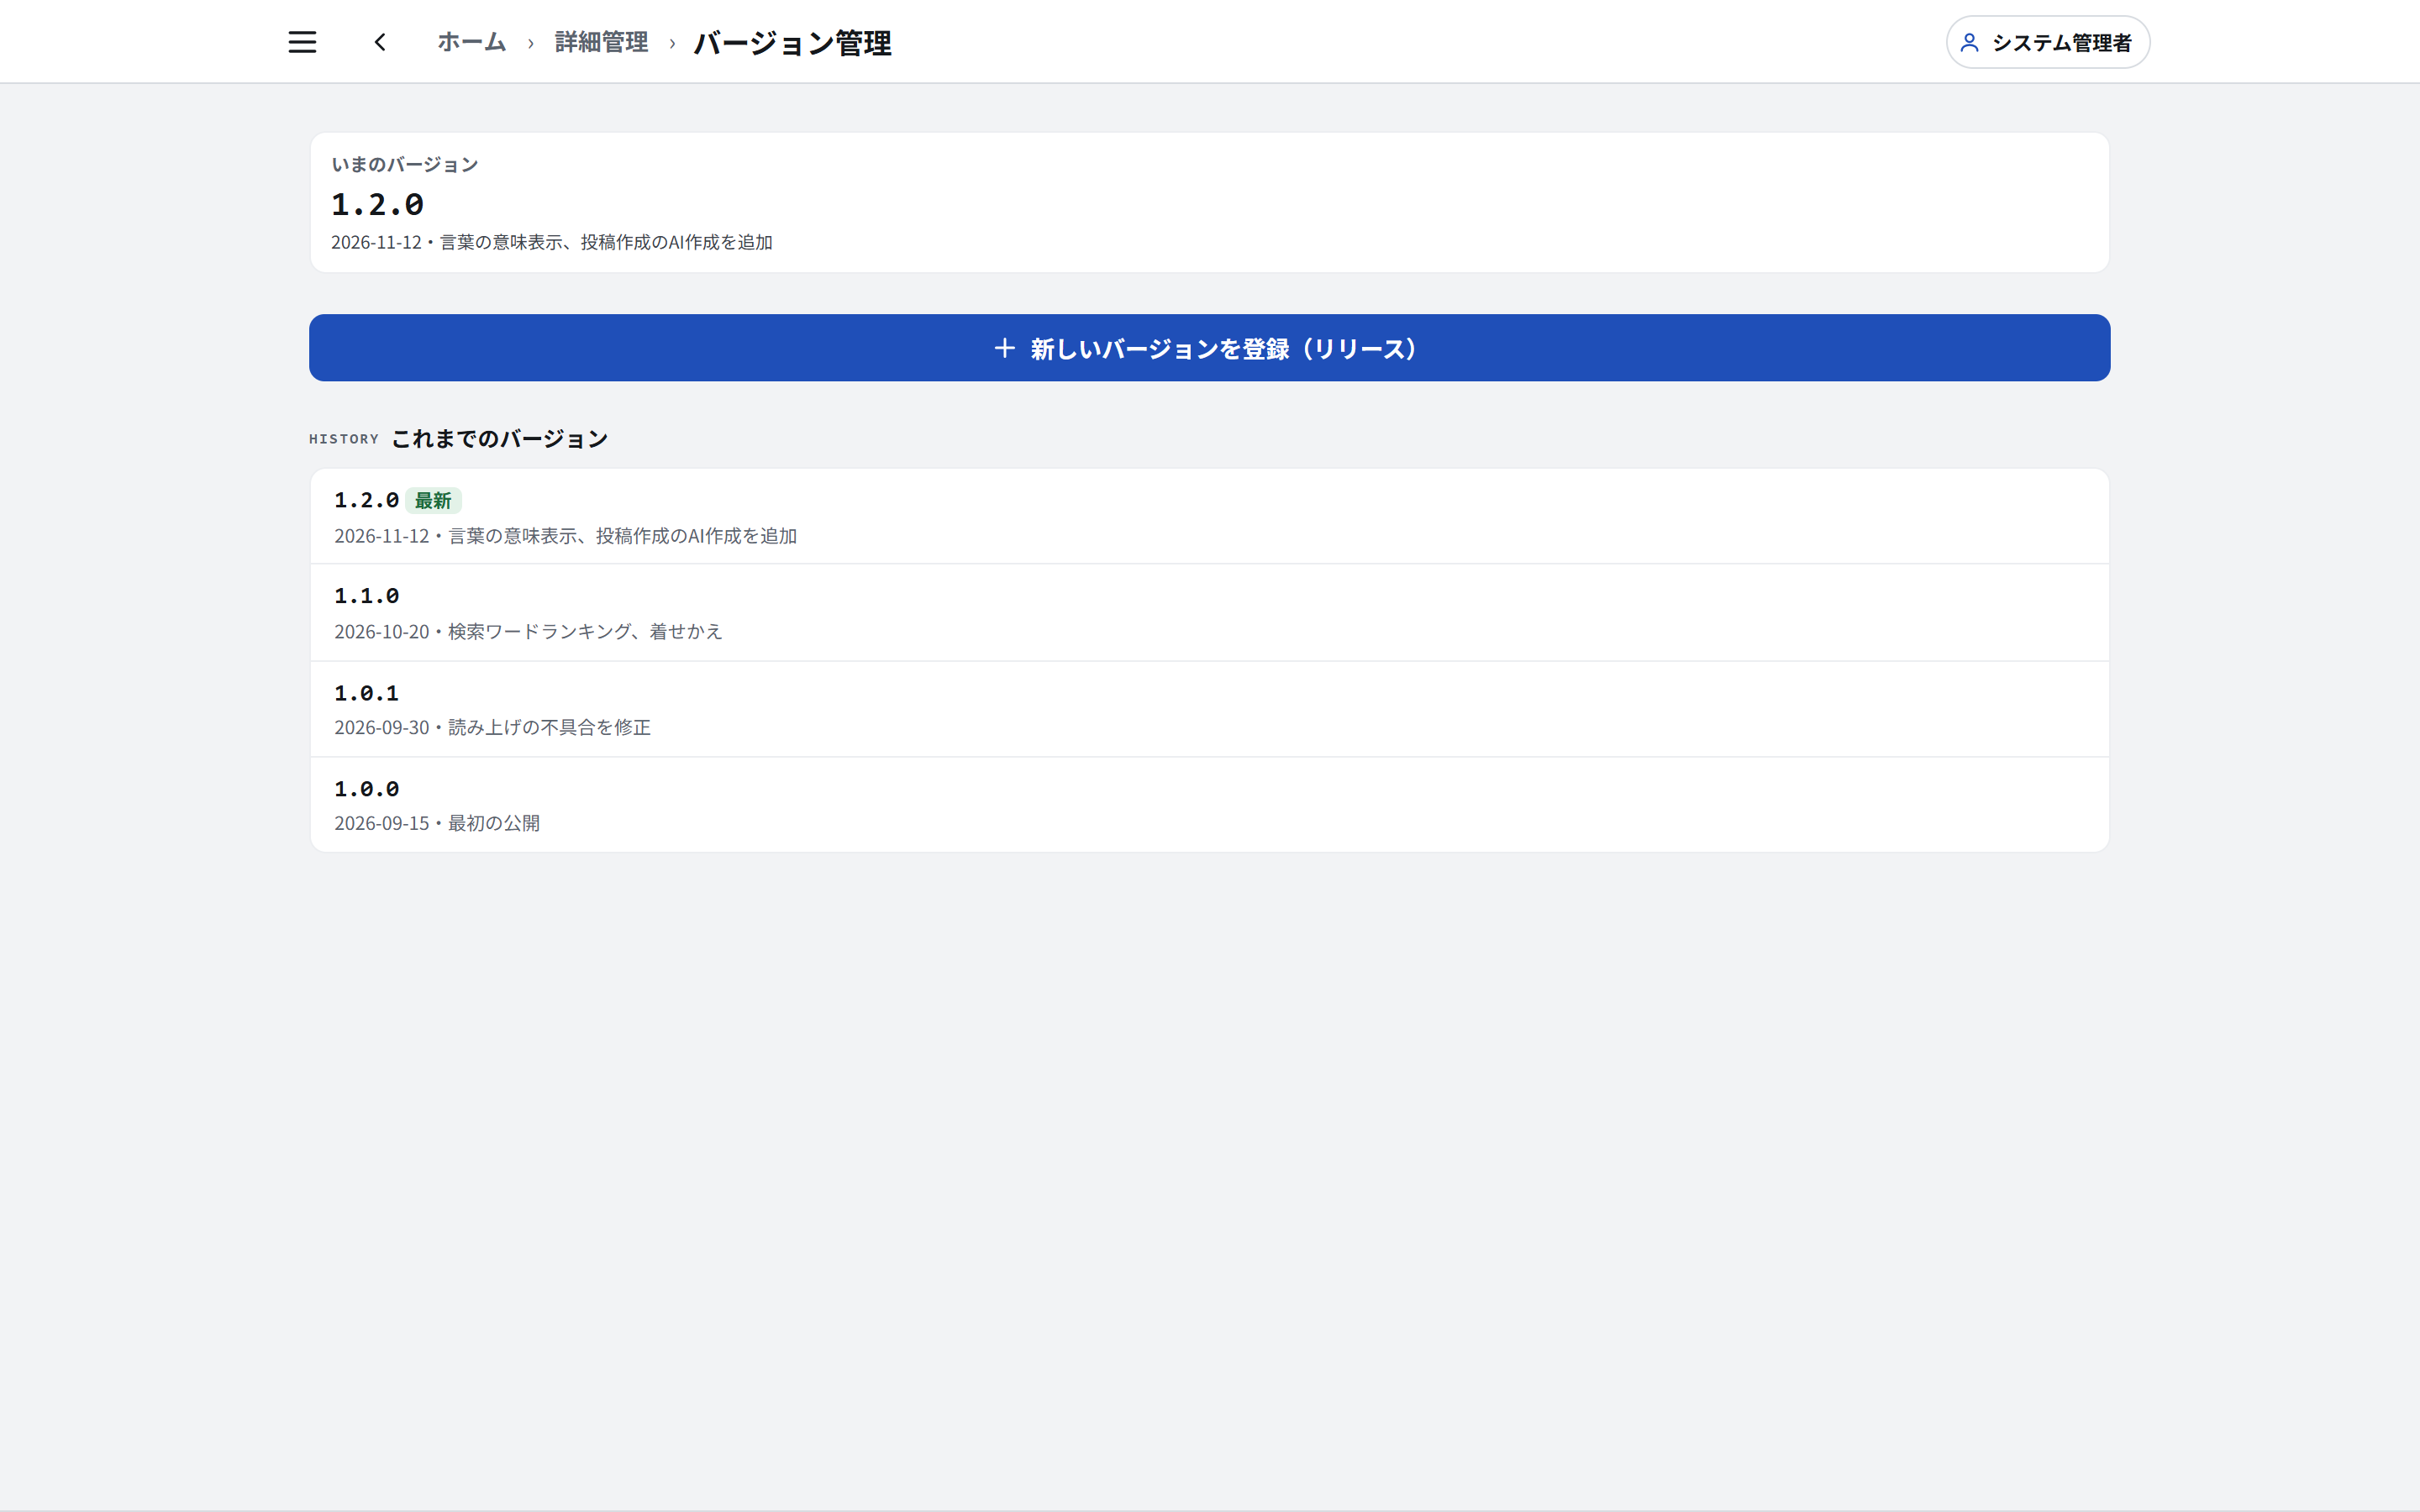
\includegraphics[width=\linewidth]{chapters/images/UI_Screen/admin/version.png}
    \caption{バージョン管理画面}
    \label{fig:ad_version}
  \end{subfigure}
  \hfill
  \begin{subfigure}[t]{0.48\linewidth}
    \centering
    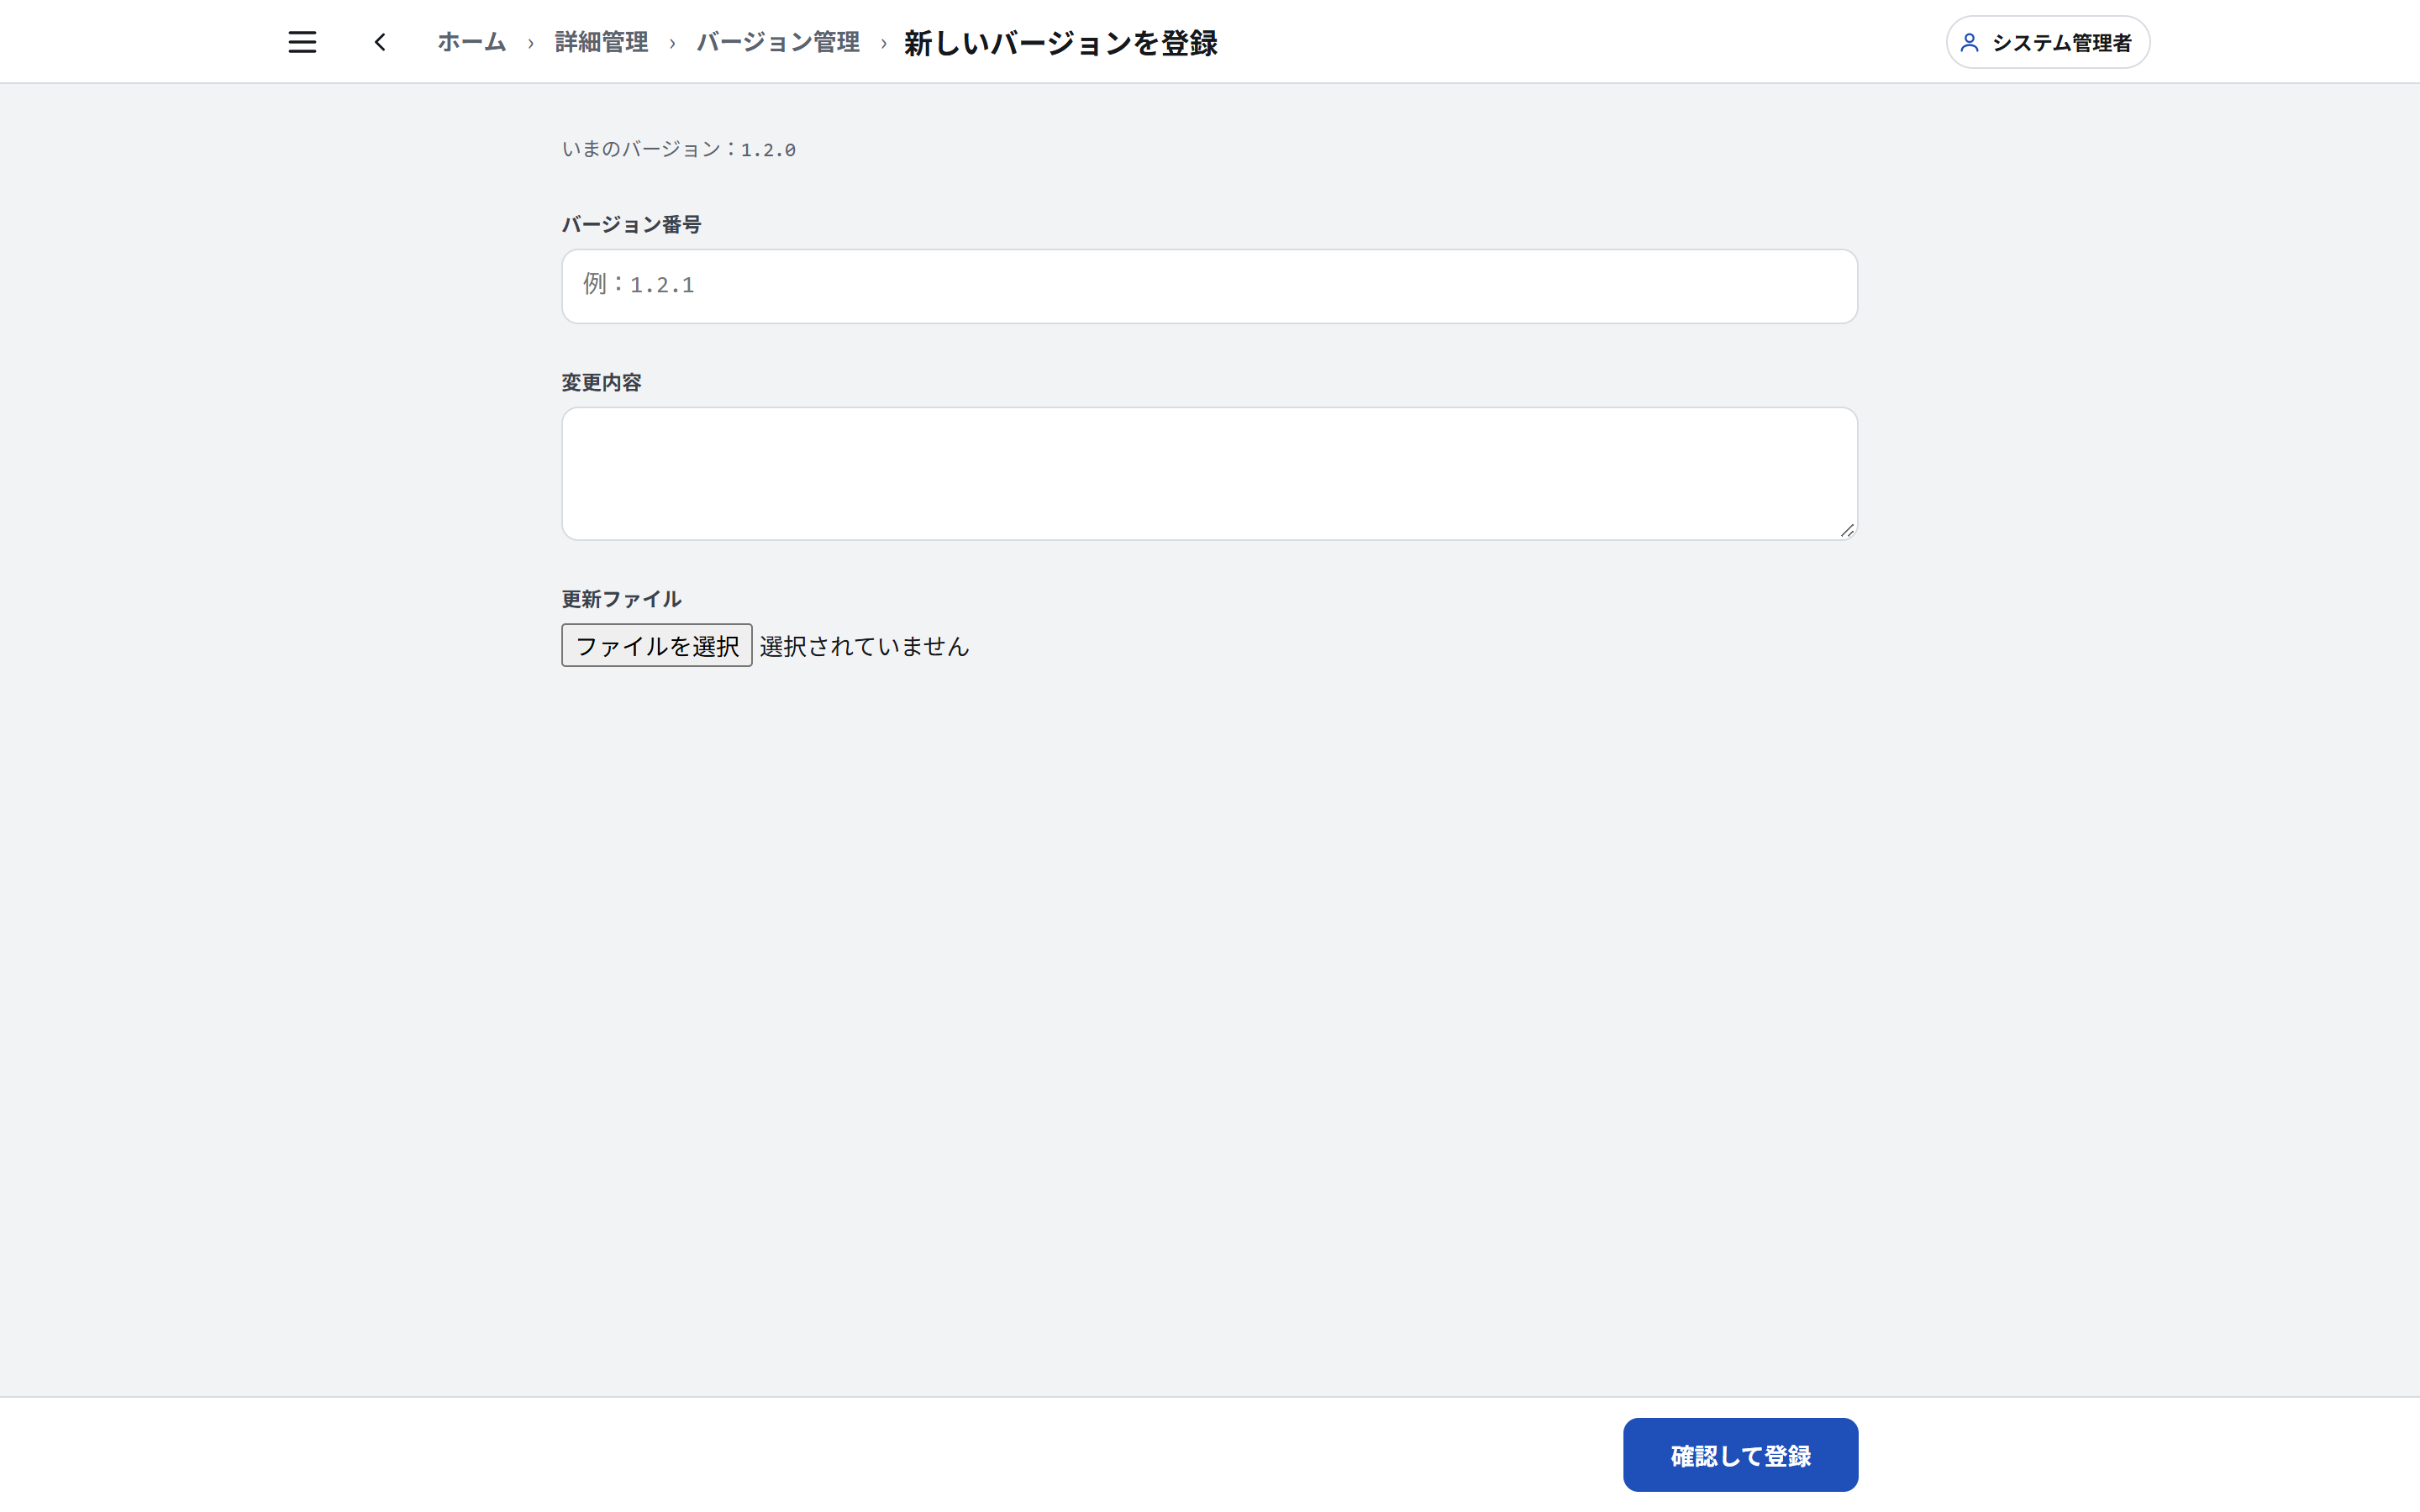
\includegraphics[width=\linewidth]{chapters/images/UI_Screen/admin/version_new.png}
    \caption{バージョン登録画面}
    \label{fig:ad_version_new}
  \end{subfigure}

  \caption{バージョン管理画面}
  \label{fig:ad_versions}
\end{figure}

図\ref{fig:ad_version}は、アプリのバージョンを管理する画面である。現在のバージョンと公開日・変更内容、これまでのバージョンの履歴が表示される。「新しいバージョンを登録（リリース）」をクリックすると、バージョン登録画面へ遷移する。

図\ref{fig:ad_version_new}は、アプリの新しいバージョンを登録する画面である。現在のバージョンが表示され、バージョン番号・変更内容・更新ファイルを入力して「確認して登録」をクリックすると登録することができる。